%\documentclass[]{report}
\documentclass[12pt,a4paper,twoside,openright]{report}
\usepackage[a4paper,top=2.2cm,bottom=2.5cm,left=2.3cm,right=2.3cm,includeheadfoot]{geometry}
\usepackage{longtable} 
\usepackage{booktabs}
\usepackage{bm}
\usepackage{amssymb}
% The following packages can be found on http:\\www.ctan.org
\usepackage{graphics} % for pdf, bitmapped graphics files
\usepackage{epsfig} % for postscript graphics files
\usepackage{mathptmx} % assumes new font selection scheme installed
\usepackage{times} % assumes new font selection scheme installed
\usepackage{amsmath} % assumes amsmath package installed
%\usepackage{amssymb}  % assumes amsmath package installed
\usepackage[]{units} % units
\usepackage{algorithm} % algorithms
\usepackage[noend]{algpseudocode} % algorithms
\algrenewcommand\algorithmicrequire{\textbf{Given: }} % algorithms
\DeclareMathAlphabet{\mathcal}{OMS}{cmsy}{m}{n} % calligraphic fonts in math mode
\usepackage{booktabs} % hübsche Tabellen
\usepackage{graphicx}
\usepackage{multirow}
\usepackage{adjustbox}
\usepackage{cancel}
\usepackage{needspace}
\usepackage{tikz}


% #1 colour, #2 marker path centred at origin
\newcommand{\mlLegendLine}[2]{%
    \tikz[baseline=-0.6ex, line width=0.6pt]{%
        \draw[#1] (0,0) -- (0.5,0);
        \begin{scope}[shift={(0.25,0)}] \draw[#1] #2; \end{scope}}}

% 1. Blue circle (-10°)
\DeclareRobustCommand{\mlBlueCircle}{\mlLegendLine{mlblue}{(0,0) circle (1.7pt)}}
% 2. Orange asterisk (-7°)
\DeclareRobustCommand{\mlOrangeStar}{\mlLegendLine{mlorange}{%
        (-2pt,0) -- (2pt,0) (0,-2pt) -- (0,2pt) (-1.4pt,-1.4pt) -- (1.4pt,1.4pt) (-1.4pt,1.4pt) -- (1.4pt,-1.4pt)}}
% 3. Yellow line, no marker (-3°)
\DeclareRobustCommand{\mlYellowLine}{\mlLegendLine{mlyellow}{}}
% 4. Purple cross (0°)
\DeclareRobustCommand{\mlPurpleCross}{\mlLegendLine{mlpurple}{%
        (-1.5pt,-1.5pt) -- (1.5pt,1.5pt) (-1.5pt,1.5pt) -- (1.5pt,-1.5pt)}}
% 5. Green diamond (3°)
\DeclareRobustCommand{\mlGreenDiamond}{\mlLegendLine{mlgreen}{%
        (0,2.2pt) -- (2.2pt,0) -- (0,-2.2pt) -- (-2.2pt,0) -- cycle}}
% 6. Cyan right-pointing triangle (7°)
\DeclareRobustCommand{\mlCyanTriangle}{\mlLegendLine{mlcyan}{%
        (2.2pt,0) -- (-1.3pt,2pt) -- (-1.3pt,-2pt) -- cycle}}
% 7. Maroon upward triangle (10°)
\DeclareRobustCommand{\mlMaroonTriangle}{\mlLegendLine{mlmaroon}{%
        (0,2.2pt) -- (2pt,-1.3pt) -- (-2pt,-1.3pt) -- cycle}}

% Define the modern MATLAB RGB colors
\definecolor{mlblue}{RGB}{0,114,189}      % 1. Blue
\definecolor{mlorange}{RGB}{217,83,25}    % 2. Orange
\definecolor{mlyellow}{RGB}{237,177,32}   % 3. Yellow
\definecolor{mlpurple}{RGB}{126,47,142}   % 4. Purple
\definecolor{mlgreen}{RGB}{119,172,48}    % 5. Green
\definecolor{mlcyan}{RGB}{77,190,238}     % 6. Light Blue / Cyan
\definecolor{mlmaroon}{RGB}{162,20,47}    % 7. Maroon

\definecolor{mlblack}{RGB}{0,0,0}    % Black


\definecolor{mlred}{rgb}{1,0,0}      % MATLAB 'r'
\definecolor{mlpink}{rgb}{1,0,1}     % MATLAB 'm' (magenta)
\definecolor{mldarkgreen}{rgb}{0,0.6,0}     % MATLAB green
\definecolor{mldarkblue}{rgb}{0,0,0.8}     % MATLAB blue
\definecolor{mldarkred}{rgb}{0.8,0,0}     % MATLAB red

\definecolor{mloldblue}{rgb}{0,0,1}     % MATLAB old blue
\definecolor{mloldgreen}{rgb}{0,1,0}     % MATLAB old green

\tikzset{mlline/.style={line width=1.7pt}}

% Create convenient inline legend line commands
\DeclareRobustCommand{\mlBlue}{\tikz[baseline=-0.6ex]\draw[mlblue, mlline] (0,0) -- (0.4,0);}
\DeclareRobustCommand{\mlOrange}{\tikz[baseline=-0.6ex]\draw[mlorange, mlline] (0,0) -- (0.4,0);}
\DeclareRobustCommand{\mlYellow}{\tikz[baseline=-0.6ex]\draw[mlyellow, mlline] (0,0) -- (0.4,0);}
\DeclareRobustCommand{\mlPurple}{\tikz[baseline=-0.6ex]\draw[mlpurple, mlline] (0,0) -- (0.4,0);}
\DeclareRobustCommand{\mlGreen}{\tikz[baseline=-0.6ex]\draw[mlgreen, mlline] (0,0) -- (0.4,0);}
\DeclareRobustCommand{\mlCyan}{\tikz[baseline=-0.6ex]\draw[mlcyan, mlline] (0,0) -- (0.4,0);}
\DeclareRobustCommand{\mlMaroon}{\tikz[baseline=-0.6ex]\draw[mlmaroon, mlline] (0,0) -- (0.4,0);}

\DeclareRobustCommand{\mlBlackDashed}{\tikz[baseline=-0.6ex]\draw[black, mlline, dash pattern=on 3pt off 2pt] (0,0) -- (0.4,0);}

%\definecolor{mlgray}{RGB}{0.8,0.8,0.8}  % Gray
\definecolor{mlgray}{rgb}{0.5,0.5,0.5}  % Gray
\DeclareRobustCommand{\mlGrayDashed}{\tikz[baseline=-0.6ex]\draw[mlgray, mlline, dash pattern=on 3pt off 2pt] (0,0) -- (0.4,0);}
\DeclareRobustCommand{\mBlack}{\tikz[baseline=-0.6ex]\draw[mlblack, mlline] (0,0) -- (0.4,0);}
\DeclareRobustCommand{\mlRed}{\tikz[baseline=-0.6ex]\draw[mlred, mlline] (0,0) -- (0.4,0);}
\DeclareRobustCommand{\mlDarkGreen}{\tikz[baseline=-0.6ex]\draw[mldarkgreen, mlline] (0,0) -- (0.4,0);}
\DeclareRobustCommand{\mlGray}{\tikz[baseline=-0.6ex]\draw[mlgray, mlline] (0,0) -- (0.4,0);}

\DeclareRobustCommand{\mlPink}{\tikz[baseline=-0.6ex]\draw[mlpink, mlline] (0,0) -- (0.4,0);}
\DeclareRobustCommand{\mlOldBlue}{\tikz[baseline=-0.6ex]\draw[mloldblue, mlline] (0,0) -- (0.4,0);}
\DeclareRobustCommand{\mlOldGreen}{\tikz[baseline=-0.6ex]\draw[mloldgreen, mlline] (0,0) -- (0.4,0);}

\DeclareRobustCommand{\mlBlueDashDot}{\tikz[baseline=-0.6ex]\draw[mlblue, mlline, dash pattern=on 4pt off 1.5pt on 1pt off 1.5pt] (0,0) -- (0.4,0);}
%\DeclareRobustCommand{\mlYellowDotted}{\tikz[baseline=-0.6ex]\draw[mlyellow, mlline, line cap=round, dash pattern=on 0pt off 3pt] (0,0) -- (0.4,0);}
\DeclareRobustCommand{\mlYellowDotted}{\tikz[baseline=-0.6ex]\draw[mlyellow, mlline, dash pattern=on 1.5pt off 1.5pt] (0,0) -- (0.4,0);}
\DeclareRobustCommand{\mlGreenDotted}{\tikz[baseline=-0.6ex]\draw[mlgreen, mlline, dash pattern=on 1.5pt off 1.5pt] (0,0) -- (0.4,0);}

\DeclareRobustCommand{\mlPurpleDashDot}{\tikz[baseline=-0.6ex]\draw[mlpurple, mlline, dash pattern=on 4pt off 1.5pt on 1pt off 1.5pt] (0,0) -- (0.4,0);}
\DeclareRobustCommand{\mlPinkDotted}{\tikz[baseline=-0.6ex]\draw[mlpink, mlline, dash pattern=on 1.5pt off 1.5pt] (0,0) -- (0.4,0);}
\DeclareRobustCommand{\mlGreenDashed}{\tikz[baseline=-0.6ex]\draw[mlgreen, mlline, dash pattern=on 3pt off 2pt] (0,0) -- (0.4,0);}

\DeclareRobustCommand{\mlOldBlueDashed}{\tikz[baseline=-0.6ex]\draw[mloldblue, mlline, dash pattern=on 3pt off 2pt] (0,0) -- (0.4,0);}
\DeclareRobustCommand{\mlOldBlueeDashDot}{\tikz[baseline=-0.6ex]\draw[mloldblue, mlline, dash pattern=on 4pt off 1.5pt on 1pt off 1.5pt] (0,0) -- (0.4,0);}
\DeclareRobustCommand{\mlYellowDashDot}{\tikz[baseline=-0.6ex]\draw[mlyellow, mlline, dash pattern=on 4pt off 1.5pt on 1pt off 1.5pt] (0,0) -- (0.4,0);}


\DeclareRobustCommand{\mlDarkBlueDashed}{\tikz[baseline=-0.6ex]\draw[mldarkblue, mlline, dash pattern=on 3pt off 2pt] (0,0) -- (0.4,0);}
\DeclareRobustCommand{\mlDarkRedDashed}{\tikz[baseline=-0.6ex]\draw[mldarkred, mlline, dash pattern=on 3pt off 2pt] (0,0) -- (0.4,0);}
\DeclareRobustCommand{\mlPurpleDashed}{\tikz[baseline=-0.6ex]\draw[mlpurple, mlline, dash pattern=on 3pt off 2pt] (0,0) -- (0.4,0);}


% #1 colour, #2 line pattern, #3 marker path (centred at origin)
\newcommand{\mlMarkerLine}[3]{%
    \tikz[baseline=-0.6ex]{%
        \draw[#1, mlline, #2] (0,0) -- (0.7,0);
        \begin{scope}[shift={(0.35,0)}] \draw[#1, line width=0.9pt, fill=white] #3; \end{scope}}}

\DeclareRobustCommand{\mlBlueDashDotSquare}{\mlMarkerLine{mloldblue}{dash pattern=on 4pt off 1.5pt on 1pt off 1.5pt}{(-2.2pt,-2.2pt) rectangle (2.2pt,2.2pt)}}
\DeclareRobustCommand{\mlDarkGreenDashedDiamond}{\mlMarkerLine{mldarkgreen}{dash pattern=on 3pt off 2pt}{(0,3pt) -- (3pt,0) -- (0,-3pt) -- (-3pt,0) -- cycle}}
\DeclareRobustCommand{\mlRedCircle}{\mlMarkerLine{mlred}{}{(0,0) circle (2.4pt)}}

\definecolor{mlmeshblue}{rgb}{0,0,0.8}
\definecolor{mlmeshgray}{rgb}{0.7,0.7,0.7}

\DeclareRobustCommand{\mlPrimaryMesh}{\tikz[baseline=-0.6ex]\draw[mlmeshblue, line width=0.9pt] (0,-0.09) rectangle (0.4,0.09);}
\DeclareRobustCommand{\mlSecondaryMesh}{\tikz[baseline=-0.6ex]\draw[mlmeshgray, line width=0.9 pt] (0,-0.09) rectangle (0.4,0.09);}



%\DeclareRobustCommand{\mlBlackDashed}{\tikz[baseline=-0.6ex]\draw[black, thick, dash pattern=on 2pt off 1.5pt] (0,0) -- (0.4,0);}


% Centered legend line helper
%\newcommand{\mlBlue}{\textcolor{mlblue}{\raisebox{0.5ex}{\rule{0.4cm}{1.5pt}}}}
%\newcommand{\mlOrange}{\textcolor{mlorange}{\raisebox{0.5ex}{\rule{0.4cm}{1.5pt}}}}


% Helper macro for a line segment with a marker in the center
\newcommand{\mlLegendItem}[2]{% 
    \textcolor{#1}{\raisebox{0.3ex}{%
            \rule{0.15cm}{1.2pt}%
            \hspace{1pt}#2\hspace{1pt}%
            \rule{0.15cm}{1.2pt}%
    }}%
}


\usepackage[table]{xcolor}

% In your preamble:
\usepackage{etoolbox}
\patchcmd{\listoftables}{\chapter*}{\section*}{}{}  % demote to section, no new page
\patchcmd{\listoffigures}{\chapter*}{\section*}{}{}


\usepackage{fancyhdr}
\usepackage{emptypage}
\pagestyle{fancy}
\fancyhf{} % clear defaults
\allowdisplaybreaks

\usepackage{enumitem}
%\setlist{nosep}
%\setlist{noitemsep}
%\setlist{itemsep=0.3ex, topsep=0.ex, parsep=0pt}
\setlist{
    itemsep=0.3ex,
    parsep=0pt,
    before=\vspace{0.0ex},
    after=\vspace{0ex}
}
\setlist[itemize]{label=-}

\clubpenalty=10000
\widowpenalty=10000
\brokenpenalty=10000

%\AtBeginDocument{%
%    \setlength{\abovedisplayskip}{1.0ex}%
%    \setlength{\belowdisplayskip}{2ex}%
%    \setlength{\abovedisplayshortskip}{1.0ex}%
%    \setlength{\belowdisplayshortskip}{2ex}%
%}

\renewcommand{\topfraction}{0.9}       % Allow top floats to take up to 90% of the page
\renewcommand{\bottomfraction}{0.9}    % Allow bottom floats up to 90%
\renewcommand{\textfraction}{0.1}      % Minimum fraction of page that must be text
\renewcommand{\floatpagefraction}{0.85}% Fraction needed for a float-only page

% Define header
\fancyhead[LE,RO]{\thepage}  % page number on the outer side
\fancyhead[RE]{\leftmark}    % chapter title on even pages
\fancyhead[LO]{\rightmark}   % section title on odd pages

% Thin header rule
\renewcommand{\headrulewidth}{0.4pt}

\usepackage[authoryear,square]{natbib}
\setcitestyle{aysep={,}, brackets={[}{]}, citesep={;}, open={[}, close={]}}
\bibliographystyle{abbrvnat}

% Redefine \cite to behave like \citep
\let\cite\citep

\usepackage{amsthm}
\usepackage{bm}
\usepackage{amsmath}
\usepackage{caption}
%\usepackage{subcaption}
\usepackage{graphicx} 
\usepackage[caption=false]{subfig}
\usepackage{appendix}
% \usepackage{tocbibind} % To include "Appendices" in the table of contents
\usepackage[nottoc]{tocbibind}
\usepackage{makecell}

\usepackage{gensymb}
%\usepackage{siunitx}
%\usepackage{enumitem}

%\usepackage{url}
\usepackage[hyphens]{url}
\usepackage{hyperref}  % Hyperlinks the URLs, which also helps with breaking


\makeatletter
\renewcommand\hyper@natlinkbreak[2]{#1}
\makeatother

%\usepackage{hypernat} % Fixes the two-link issue

% Redefine \citep and \citet to wrap the whole citation in a single link
% \usepackage{xpatch}
% \xpatchcmd{\citep}{\begingroup}{\begingroup\def\hyper@linkstart##1##2{\@secondoftwo}}{}{}
%% xpatchcmd{\citet}{\begingroup}{\begingroup\def\hyper@linkstart##1##2{\@secondoftwo}}{}{}


%\usepackage{gensymb}
%\makeatletter
%\renewcommand*{\@opargbegintheorem}[3]{\trivlist
    %   \item[\hskip \labelsep{\bfseries #1\ #2}] \textit{(#3)}\ \itshape}
%\makeatother

% tikz
\graphicspath{ {Figures/} }
\usepackage{chngcntr}
\usepackage{pgfplots}	%for Matlab2Tikz
\usepackage{enumitem}
% preamble (main language last):
\usepackage[ngerman,english]{babel}

\usepgfplotslibrary{external}
% \tikzexternalize[prefix=figures/tikz/, shell escape=-enable-write18]	%!!Important! compile with: latex -enable-write18 on windows with MikTex
\newcommand{\atikz}[2]{\scalebox{#1}{\input{"figures/#2.tikz"}}}
%\input{"legend.tex"}

\newtheorem{theorem}{Theorem}
\newtheorem{remark}{Remark}
\newtheorem{lemma}{Lemma}
\newtheorem{definition}{Definition}

\newcommand{\Rho}{\mathsf{P}}
\newcommand{\trp}{T}
\newcommand{\ones}{\textnormal{\textbf{1}}}
\newcommand{\diag}{\textnormal{diag}}

\usepackage[T1]{fontenc}
\usepackage{microtype}

%\leftmargin=-1em
%\setlist
%\nosep
\hypersetup{hidelinks} 


% Title Page
\title{Quasi-Linear Parameter-Varying and Koopman Model Predictive Control for Wind Energy Systems}
\author{Antje Dittmer}

\raggedbottom

\begin{document}
   % \maketitle
    \makeatletter
    \begin{titlepage}
        \begin{center}
            \vspace*{1cm}
            \LARGE
            \textbf{\@title}
            
            \vspace{2.5cm}
            \large
            \textbf{Dem Promotionsausschuss der\\
                Technischen Universität Hamburg}\\[1ex]
            zur Erlangung des akademischen Grades\\[1ex]
            Doktor-Ingenieurin (Dr.-Ing.)\\[5ex]
            vorgelegte Dissertation
            
            \vspace{1.5cm}
            von\\ \@author
            
            \vspace{2cm}
            aus\\ Wedel
            
            \vspace{2cm}
            2026 %\@date
        \end{center}
        \vfill
        Betreuer: Prof.\ Dr.\ Herbert Werner
    \end{titlepage}
    \makeatother
    

 \clearpage
 \pagestyle{empty}   % no page numbers in the front matter
 ~
% \clearpage
 % \paragraph{Use of AI tools.}
During the preparation of this thesis, the AI assistant Claude (Anthropic), including the coding assistant Claude Code, was used under the author's direction as a programming and writing aid. Its use comprised:
\begin{itemize}
    \item \textbf{Code:} implementation and modification of MATLAB code in the author's GitHub repositories, e.g.,
    \begin{itemize}
        \item for the wind turbine controller studies of Chapter~\ref{sec:Application to Wind Turbine Control4}: the design of filters and additional states included in the predictive controller to improve its performance, the retuning of controller gains, the combination of the predictive controller with the individual pitch controller, and the re-evaluation of the newly designed and optimized controllers with the criteria defined in this thesis;
        \item for the wind farm controller studies of Chapter~\ref{sec:ApplicationtoWindFarmControl}: the redesign of the system identification signals; the estimation of the effective wind speeds from the turbine powers, which makes the closed-loop operation independent of wind speed measurements; a redesigned sensitivity study of the adaptive farm controller's parameters; a redesign of the nonlinear features as functions of the filtered control signals for the combined thrust and yaw farm controller, which are included as states of the model, and the adaptation of the corresponding MPC prediction to the updated model.
    \end{itemize}
    The figures and tables of the simulation results in this thesis were generated directly from the simulation data with MATLAB scripts of this code.
    \item \textbf{Text:} review of the chapters for consistency between text, equations, tables, and code; proofreading and language editing; and suggestions for passages, captions, and revised versions of sections of Chapters~1 to~6.
\end{itemize}
In addition, the author used ChatGPT, Gemini, and Perplexity for language editing, for support in generating and revising the MATLAB scripts used to produce the figures and tables, and for literature searches. All results obtained with AI tools were carefully reviewed and verified by the author. Some models were proposed or refined with the help of the AI tools; their evaluation and selection, the design decisions, and the conclusions are the author's. Suggested text was reviewed, revised, and integrated by the author, who is responsible for the entire content of this thesis.


 
 
 
    \cleardoublepage
    \begin{abstract}
        

        
          Over the past two decades, wind turbines have significantly increased in size. Ensuring their economic, fully automatic operation in varying wind conditions has become more challenging due to larger towers and rotors with longer, more slender blades. The increasing number of turbines in wind farms, sometimes a few hundred, and their close spacing, as areas suitable for wind energy are limited, further complicate this task. Not only is individual wind turbine control difficult, but wind farm control is even more so, as efficient use of space necessitates accounting for wake interactions.
          
        In this thesis, Model Predictive Control (MPC) is used to design algorithms for wind turbine and wind farm control, aiming to minimize the Levelized Cost of Energy~(LCoE). The goal is to maximize power yield while minimizing mechanical loads and keeping actuator movements within their limits and as small as possible. For individual Wind Energy Conversion Systems~(WECS), this involves maximizing energy extraction up to the rated wind speed and pitching the blades above this speed to lower mechanical loads and maintain constant power output.
           
    For wind turbine control, a velocity-based quasi-Linear Parameter-Varying Model Predictive Control (qLMPC) algorithm is implemented for the first time in this thesis as a Multiple-Input Multiple-Output (MIMO) controller covering the turbine's entire operating range. Two quasi-Linear Parameter-Varying~(qLPV) turbine models, one derived using Lagrange's equations, are developed for controller synthesis. This new qLMPC strategy is compared to state-of-the-art Collective Pitch Control~(CPC) and Individual Pitch Control~(IPC) using Damage Equivalent Loads~(DEL), power fluctuations, and actuator activity as evaluation criteria. Additionally, an enhanced turbine model with Trailing Edge Flaps (TEF) is developed, and the combination of IPC and TEF control achieves a slightly larger blade load reduction than IPC alone at considerably lower pitch actuator power.
        
        

For wind farm control, a data-driven approach models wake interactions between turbines. Data from a simulation model is used to construct Koopman matrices, finite-dimensional representations of the Koopman operator, to derive models for MPC of a two-turbine wind farm. The lifting functions are carefully selected based on physical relationships governing wind, wake interactions, and power extraction from the wind by WECS. Two Koopman models are designed: one predicts the effective wind speeds at the turbines, from which the farm power is derived using known physical relationships, while the second predicts the farm power directly. Both Koopman models use only the control signals and the measured turbine powers, which eliminates the need for wind measurements in closed loop while maintaining acceptable grid power reference tracking. An efficient online adaptive controller for wind farm thrust control is demonstrated, which adapts to freestream wind conditions not contained in the training data. Combining Wake Redirection Control (WRC) with thrust control increases the steady-state farm power compared with the greedy baseline and considerably reduces the tracking error for power references above the greedy power. Both wind turbine and wind farm control designs are formulated as Quadratic Programming (QP) problems to ensure real-time capability.
\end{abstract}
\cleardoublepage
\begin{otherlanguage}{ngerman}
{\renewcommand{\abstractname}{Kurzfassung}
    \begin{abstract}
In den letzten zwei Jahrzehnten sind Windenergieanlagen (WEA) deutlich größer geworden. Höhere Türme und Rotoren mit längeren, schlankeren Blättern erschweren ihren wirtschaftlichen, vollautomatischen Betrieb unter wechselnden Windbedingungen. Hinzu kommen die zunehmende Anzahl von Anlagen in Windparks, teilweise mehrere hundert, sowie ihre geringen Abstände aufgrund begrenzter geeigneter Flächen. Noch anspruchsvoller als die Regelung einzelner WEA ist die Windparkregelung, da eine effiziente Flächennutzung die Berücksichtigung von Nachlaufwechselwirkungen erfordert.

In dieser Arbeit wird modellprädiktive Regelung (MPC) für den Entwurf von Algorithmen zur WEA- und Windparkregelung eingesetzt, mit dem Ziel, die Stromgestehungskosten (LCoE) zu minimieren. Dabei soll der Energieertrag maximiert, die mechanischen Lasten minimiert und die Stellbewegungen innerhalb ihrer Grenzen und möglichst gering gehalten werden. Für einzelne WEA bedeutet dies, unterhalb der Nennwindgeschwindigkeit die Energieentnahme zu maximieren und oberhalb die Blätter zu verstellen, um die Lasten zu reduzieren und die Leistung konstant zu halten.

Für die Anlagenregelung wird in dieser Arbeit erstmals ein geschwindigkeitsbasierter quasi-linear parameterveränderlicher modellprädiktiver Regelungsalgorithmus (qLMPC) als Mehrgrößenregler (MIMO) für den gesamten Betriebsbereich der Anlage umgesetzt. Für den Reglerentwurf werden zwei quasi-linear parameterveränderliche (qLPV-)Modelle entwickelt, von denen eines auf den Lagrange-Gleichungen basiert. Die qLMPC wird mit der kollektiven (CPC) und der individuellen Blattverstellung (IPC) nach dem Stand der Technik verglichen, wobei schadensäquivalente Lasten (DEL), Leistungsschwankungen und Stellaktivität als Bewertungskriterien dienen. Zusätzlich wird ein Anlagenmodell mit Hinterkantenklappen (TEF) entwickelt. Die Kombination von IPC und TEF-Regelung erreicht eine etwas größere Reduktion der Blattlasten als IPC allein bei deutlich geringerer Stellleistung der Blattverstellung.

Für die Windparkregelung werden die Nachlaufwechselwirkungen zwischen den Anlagen datengetrieben modelliert. Aus Simulationsdaten werden Koopman-Matrizen, endlichdimensionale Darstellungen des Koopman-Operators, bestimmt und daraus Modelle für die MPC eines Windparks mit zwei Anlagen abgeleitet. Die Lifting-Funktionen werden auf Grundlage physikalischer Zusammenhänge zwischen Wind, Nachlaufwechselwirkungen und der Leistungsentnahme der WEA ausgewählt. Es werden zwei Koopman-Modelle entworfen: Das erste prädiziert die effektiven Windgeschwindigkeiten an den Anlagen, aus denen die Parkleistung über bekannte physikalische Zusammenhänge berechnet wird, das zweite prädiziert die Parkleistung direkt. Beide Modelle verwenden ausschließlich die Stellsignale und die gemessenen Anlagenleistungen, sodass im geschlossenen Regelkreis keine Windmessungen erforderlich sind und dennoch eine akzeptable Nachführung der Netzleistungsvorgabe erreicht wird. Ein im Betrieb adaptierender Regler für die Schubregelung im Windpark passt sich an Anströmbedingungen an, die in den Trainingsdaten nicht enthalten sind. Die Kombination von Nachlaufablenkung (WRC) und Schubregelung erhöht die stationäre Parkleistung gegenüber dem Betrieb mit maximaler Einzelleistung (Greedy-Betrieb) und verringert den Folgefehler bei Leistungsvorgaben oberhalb der Greedy-Leistung deutlich. Anlagen- und Windparkregelung werden als quadratische Optimierungsprobleme (QP) formuliert, um die Echtzeitfähigkeit sicherzustellen.
  \end{abstract}}
\end{otherlanguage}

\cleardoublepage
\pagestyle{fancy}   % normal headers with page numbers from here on

\tableofcontents
    
\makeatletter
\begingroup
\let\addcontentsline\@gobblethree

%\listoffigures
%\listoftables
\endgroup
\makeatother

    \section*{List of Symbols}
\subsection*{Latin Characters}
\begingroup
\renewcommand{\arraystretch}{0.88}
\begin{longtable}{lll}
    % \caption*{Latin Characters}
    \label{tab:SymbolsLatinCharacters}\\
    Symbol & Meaning & Unit \\
    \toprule
    \endfirsthead
    \toprule
    \endhead
    \bottomrule \multicolumn{3}{r}{\emph{continued on the next page}}
    \endfoot
    \bottomrule
    \endlastfoot
    \hspace{1.7cm} & \hspace{8.8cm} & \hspace{2.4cm} \kill
    $\bm{0}_{\mathrm{d_1}\times{\mathrm{d_2}}}$ & Zero matrix of dimension $\mathrm{d_1}\times {\mathrm{d_2}}$ & -- \\
    $\bm{1}_{\mathrm{d}}$ & Vector of dimension $\mathrm{d} \times 1$ with all elements equal to 1& -- \\
    $A$ & Area & $\mathrm{m}^2$ \\
    $\bm{A}$ & System matrix & [...] \\
    $a$ & Axial induction factor & -- \\
    $a^{\prime}$ & Angular induction factor & -- \\
    $B$ & Damping factor & [...] \\
    $\bm{B}$ & Input matrix & [...] \\
    $b$ & Wake expansion coefficient & -- \\
    $C$ & Optimization criterion & -- \\
    $\bm{C}$ & Output matrix & [...] \\
    $\mathbf{C}$ & Damping matrix & [...] \\
    $C_{\text{WB}}$ & Scaling factor of the Weibull distribution & -- \\
    $c$ & Blade chord & $\mathrm{m}$ \\
    $c$ & Coefficient & -- \\
    $D$ & Damage fraction & -- \\
    $\bm{D}$ & Through-put matrix & [...] \\
    $D_r$ & Rotor diameter & $\mathrm{m}$ \\
    $\bm{d}$ & Disturbance input vector & --  \\
    $E_d$ & Dissipation function & $\mathrm{W}$\\
    $E_k$ & Kinetic energy & $\mathrm{J}$\\
    $E_p$ & Potential energy & $\mathrm{J}$\\
    $F_{T,r}$ & Rotor thrust & $\mathrm{N}$ \\
    $f$ & Frequency & $\mathrm{Hz}$ \\
    $G$ & Transfer function & [...] \\
    $H_t$ & Hub height & $\mathrm{m}$ \\
    $\bm{I}_\mathrm{d}$ & Identity matrix of dimension $\mathrm{d}\times {\mathrm{d}}$& -- \\
    $I_\mathrm{V}$ & Turbulence intensity & -- \\
    $J$ & Cost function & -- \\
    $J$ & Mass moment of inertia & $\mathrm{kgm}^2$ \\
    $K$ & Factor or controller gain & [...] \\
    $K$ & Stiffness factor & [...] \\
    $\mathbf{K}$ & Stiffness matrix & [...] \\
    $k_{\text{WB}}$ & Shape factor of the Weibull distribution & -- \\
    $L$ & Number of load cycles to failure & -- \\
    $l$ & Load cycle count & -- \\
    $\mathbf{M}$ & Mass matrix & [...] \\  
    $m$ & Mass & $\mathrm{kg}$ \\
    $m$ & Wöhler exponent & -- \\
    $N_g$ & Gear ratio & -- \\
    $P$ & Power & $\mathrm{W}$ \\
    $p$ & Pressure &  $\mathrm{N/m}^2$ \\
    $\mathbf{Q}$  & Force vector & [...] \\
    $R_r$ & Rotor radius & $\mathrm{m}$ \\
    $\mathbb{R}$ & Set of real numbers & -- \\
    $r$ & Radial position on blade & $\mathrm{m}$ \\
    $S$ & Moment range of a load cycle & $\mathrm{Nm}$ \\
    $s$ & Laplace variable & $\mathrm{rad/s}$ \\
    $T$ & Interval or period duration & $\mathrm{s}$ \\
    $T_r$ & Rotor torque & $\mathrm{Nm}$ \\
    $t$ & Time & $\mathrm{s}$ \\
    $\bm{u}$ & Control input vector & [...] \\
    $V$ & Absolute wind speed with $V = \sqrt{v_x^2 + v_y^2 + v_z^2}$& $\mathrm{m/s}$ \\
    $V_{\text{inflow}}$ & Inflowing wind speed at blade section &  $\mathrm{m/s}$\\
    $\bm{v}$ & Wind speed vector with $\bm{v} = [v_x\ v_y\ v_z]^T$ & $\mathrm{m/s}$ \\
    $\bm{w}$ & Input vector $\bm{w}=[\bm{u}\ \bm{d}]^T$  & [...] \\
    $x$ & Longitudinal coordinate & $\mathrm{m}$ \\
    $\bm{x}$ & State vector & [...] \\
    $y$ & Lateral coordinate & $\mathrm{m}$ \\
    $\bm{y}$ & Output vector & [...] \\
    $z$ & Vertical coordinate (height above ground) & $\mathrm{m}$ \\
\end{longtable}
\endgroup

\vspace{0.05cm}

\subsection*{Greek Characters}
\begingroup
\renewcommand{\arraystretch}{0.88}
\begin{longtable}{lll}
    % \caption*{Greek Characters}
    \label{tab:SymbolsGreekCharacters}\\
    Symbol & Meaning & Unit \\
    \toprule
    \endfirsthead
    \toprule
    \endhead
    \bottomrule \multicolumn{3}{r}{\emph{continued on the next page}}
    \endfoot
    \bottomrule
    \endlastfoot
    \hspace{1.7cm} & \hspace{8.8cm} & \hspace{2.4cm} \kill
    $\alpha$ & Angle of attack & $\mathrm{rad}$ \\
    $\alpha_{\text{shear}}$ & Wind shear exponent of the power law & -- \\
    $\beta$ & Blade pitch angle & $\mathrm{rad}$ \\
    $\beta_0$ & Collective blade pitch angle & $\mathrm{rad}$ \\
    $\beta_i$ & Individual blade pitch angle of the $i^{\text{th}}$ blade & $\mathrm{rad}$ \\
    $\gamma$ & Turbine yaw angle &  $\mathrm{rad}$ \\
    $\Delta$ & Deviation & -- \\
    $\delta$ & Standard deviation & [...] \\
    $\delta$ & Wake deflection centerline &  $\mathrm{m}$ \\
    $\delta_b$ & Blade angular out-of-plane deflection &  $\mathrm{rad}$ \\
    $\zeta$ & Damping ratio & -- \\
    $\eta$ & Efficiency & -- \\
    $\theta$ & Angle & $\mathrm{rad}$ \\
    $\kappa$ & Time constant of the generator torque actuator & $\mathrm{s}$ \\
    $\lambda$ & Tip-speed ratio & -- \\
    $\nu$ & Trigger threshold of the online model update & $\mathrm{m/s}$\\
    $\rho_a$ & Air density & $\mathrm{kg/m}^3$ \\
    $\bm{\rho}_P$ & Scheduling parameter vector & [...] \\
    $\sigma$ & Stress & $\mathrm{N/m}^2$ \\
    $\tau$ & Time constant of the pitch actuator & $\mathrm{s}$ \\
    $\varphi$ & Koopman observable &  [...] \\
    $\omega$ & Angular velocity, angular frequency & $\mathrm{rad/s}$ \\
\end{longtable}
\endgroup

\vspace{0.05cm}

\subsection*{Indices}
\begingroup
\renewcommand{\arraystretch}{0.88}
\begin{longtable}{ll}
    % \caption*{Indices}
    \label{tab:SymbolsIndices}\\
    Index & Meaning \\
    \toprule
    \endfirsthead
    \toprule
    \endhead
    \bottomrule \multicolumn{2}{r}{\emph{continued on the next page}}
    \endfoot
    \bottomrule
    \endlastfoot
    \hspace{1.7cm} & \hspace{11.6cm} \kill
    {$(\cdot)_b$} & {Blade related}\\
    {$(\cdot)_c$} & {Related to a continuous system}\\
    {$(\cdot)_D$} & {Drag}\\
    {$(\cdot)_\text{D}$} & {Differential gain}\\
    {$(\cdot)_d$} & {Related to a discrete system}\\
    {$(\cdot)_g$} & {Generator related, high-speed shaft side}\\
    {$(\cdot)_{gr}$} & {Generator related, low-speed shaft side}\\
    {$(\cdot)_\text{I}$} & {Integral gain}\\
    {$(\cdot)_\text{iNF}$} & {Inverse notch filter}\\
    {$(\cdot)_L$} & {Lift}\\
    {$(\cdot)_P$} & {Power}\\
    {$(\cdot)_\text{P}$} & {Proportional gain}\\
    {$(\cdot)_Q$} & {Torque}\\
    {$(\cdot)_r$} & {Rotor related, low-speed shaft side}\\
    {$(\cdot)_\text{ref}$} & {Reference signal}\\
    {$(\cdot)_s$} & {Drivetrain transmission related}\\
    {$(\cdot)_T$} & {Thrust}\\
    {$(\cdot)_t$} & {Tower related}\\
    {$(\cdot)_V$} & {Speed related}\\
    {$(\cdot)_\text{WF}$} & {Wind farm related}\\
    {$(\cdot)_\text{WT}$} & {Wind turbine related}\\
    {$(\cdot)_\infty$} & {Condition far ahead of the system}\\
    {$(\cdot)_{\text{-}\infty}$} & {Condition far behind the system}\\
    {$(\cdot)^*$} & {Optimal value}\\
\end{longtable}
\endgroup

\section*{Mathematical Notation}
\begingroup
\renewcommand{\arraystretch}{0.88}
\begin{longtable}{p{1.7cm} p{11.6cm}}
    \label{tab:Operators}\\
    Symbol & Meaning \\
    \toprule
    \endfirsthead
    \toprule
    \endhead
    \bottomrule \multicolumn{2}{r}{\emph{continued on the next page}}
    \endfoot
    \bottomrule
    \endlastfoot
    $\mathbb{R}^{n \times 1}$ & $n$-dimensional real column vector space \\
    $\mathbb{R}^{1 \times n}$ & $n$-dimensional real row vector space \\
    $\mathbb{R}^{\mathrm{d_1}\times \mathrm{d_2}}$ & Space of $\mathrm{d_1} \times \mathrm{d_2}$ real matrices \\
    $\mathcal{H}$ & Hilbert space; a complete inner-product space \\
    $\|A\|_F$ & Frobenius norm of matrix $A$, square root of sum of squared magnitude of matrix elements: $\left( \sum_{i,j} |a_{ij}|^2 \right)^{1/2}$ where $a_{ij}$ are the elements of $A$\\
    $\|v\|_2$ & Euclidean norm (2-norm) of vector $v$, square root of sum of squared elements: $\left( \sum_{i} |v_{i}|^2 \right)^{1/2}$ \\
    $\| v\|_{\infty} $ & Infinity norm of vector $v$, maximum absolute value of the vector elements: $\max |v_{i}|$ where $v_{i}$ are the elements of $v$\\
    $A^{\dagger}$ & Moore-Penrose pseudoinverse of matrix $A$; generalizes $(A^{T}A)^{-1}A^{T}$ if $A$ has full column rank \\
    $A^T$ & Transpose of matrix $A$ \\[4pt]
\end{longtable}
\endgroup

\section*{Abbreviations}
\begingroup
\renewcommand{\arraystretch}{0.88}
\begin{longtable}{ll}
    % \caption*{Abbreviations}
    \label{tab:SymbolsAbbreviations}\\
    Abbreviation & Meaning \\
    \toprule
    \endfirsthead
    \toprule
    \endhead
    \bottomrule \multicolumn{2}{r}{\emph{continued on the next page}}
    \endfoot
    \bottomrule
    \endlastfoot
    \hspace{1.7cm} & \hspace{11.6cm} \kill
    {1P} & {One-per-revolution frequency}\\
    {2D}  & {Two-dimensional}\\
    {2P} & {Two-per-revolution frequency}\\
    {3D}  & {Three-dimensional}\\
    {5$D$}  & {Five rotor diameters downstream}\\
    {AA} & {Actuator Activity}\\
    {AALC} & {Active Aerodynamic Load Control}\\
    {AEP} & {Annual Energy Production}\\
    {AIC} & {Axial Induction Control}\\
    {BEM} & {Blade Element Momentum}\\
    {CFD} & {Computational Fluid Dynamics}\\
    {CPC} & {Collective Pitch Control} \\
    {CPU} & {Central Processing Unit} \\
    {DEL} & {Damage Equivalent Load} \\
    {DLC} & {Design Load Case} \\
    {DLR} & {German Aerospace Center} \\
    {DMD} & {Dynamic Mode Decomposition} \\
    {DWM} & {Dynamic Wake Meandering} \\
    {EDMD} & {Extended Dynamic Mode Decomposition} \\
    {EIODMD} & {Extended Input-Output Dynamic Mode Decomposition} \\
    {FAST} & {Fatigue, Aerodynamics, Structures, and Turbulence}\\
    {GFRP} & {Glass Fiber Reinforced Polymer} \\
    {IEC} & {International Electrotechnical Commission} \\
    {IPC} & {Individual Pitch Control} \\
    {ISA} & {International Standard Atmosphere} \\
    {LCoE} & {Levelized Cost of Energy} \\
    {LES} & {Large Eddy Simulation} \\
    {lidar} & {Light Detection and Ranging}\\
    {LMI} & {Linear Matrix Inequality} \\
    {LPV} & {Linear Parameter-Varying} \\
    {LQG} & {Linear Quadratic Gaussian}\\
    {LQR} & {Linear Quadratic Regulator}\\
    {LTI} & {Linear Time-Invariant} \\
    {MBC} & {Multiblade Coordinate Transformation}\\
    {MIMO} & {Multiple-Input Multiple-Output} \\
    {MPC} & {Model Predictive Control} \\
    {NMPC} & {Nonlinear Model Predictive Control} \\
    {NREL} & {National Renewable Energy Laboratory} \\
    {NSE} & {Navier-Stokes Equations}\\
    {ODE} & {Ordinary Differential Equation}\\
    {OoP} & {Out-of-Plane}\\
    {PDE} & {Partial Differential Equation}\\
    {PI}  & {Proportional-Integral (controller)}\\
    {PID}  & {Proportional-Integral-Derivative (controller)}\\
    {PSD}  & {Power Spectral Density}\\
    {qLMPC}  & {Quasi-Linear (Parameter-Varying) Model Predictive Control}\\
    {qLPV}  & {Quasi-Linear Parameter-Varying}\\
    {QP}  & {Quadratic Programming}\\
    {SISO} & {Single-Input Single-Output} \\
    {TE} & {Tracking Error} \\
    {TEF} & {Trailing Edge Flap} \\
    {TEFC} & {Trailing Edge Flap Control}\\
    {TU Delft} & {Delft University of Technology} \\
    {VAF} & {Variance Accounted For}\\
    {WECS} & {Wind Energy Conversion System} \\
    {WFSim} & {Wind Farm Simulator} \\
    {WRC} & {Wake Redirection Control} \\
    {WRC-AIC} & {Combined Wake Redirection and Axial Induction Control} \\
\end{longtable}
\endgroup
    \chapter{Introduction}
\label{sec:Introduction}

\section{Motivation} %Wind Energy Conversion System Control} 
Wind energy plays a significant role in Germany's renewable energy landscape and provides a critical contribution to the national energy transition, with the share of electricity production from wind having increased from 1.6\% in 2000 to 27.2\% in~2025~\cite{EmberEI2026}. Wind turbines, also called Wind Energy Conversion Systems (WECS), help to meet a still increasing power demand sustainably. Unlike conventional energy sources, they neither emit greenhouse gases nor produce radioactive waste. A trend toward larger wind turbines maximizes energy yield per unit, thus enhancing the economic feasibility of wind power by lowering the Levelized Cost of Energy (LCoE). However, larger wind turbines necessitate efforts to minimize structural loads. This can be achieved both through optimized tower and blade designs~\cite{modelling2010006, Jasa_2022} as well as efficient control strategies~\cite{pao2011control}. %\cite{irena2023renewable}.  8.4\% in 2013

Apart from its low life-cycle carbon emissions, onshore wind energy has the additional advantage of having a very low LCoE value. It had the lowest global weighted-average cost of all renewable generation technologies in 2024, at USD~0.034/kWh, a decrease of 70\% since 2010~\cite{IRENA2025}. In Germany, onshore wind and ground-mounted
photovoltaics are the lowest-cost options among all new power plants: the mean costs of gas,
coal and nuclear generation are two to five times higher~\cite{Kost2024LCOE}. Moreover,
simulations and field tests show that improved turbine and wind farm operation offers the
potential to reduce the LCoE even further, concretely by increasing energy production, by
decreasing structural loads, or by both~\cite{vali2017adjointbasedmodel, houck2022review}.

The research wind farm WiValdi, shown in Figure~\ref{fig:WiValdi}, is instrumented to measure wind turbine and wind farm behavior under real inflow conditions. It is operated by the German Aerospace Center (Deutsches Zentrum für Luft- und Raumfahrt, DLR) together with its partners in the Research Alliance Wind Energy (Forschungsverbund Windenergie). Load-alleviation methods at the turbine and farm levels and increased farm-level power output are among the research
topics, see~\cite{WiValdiResearchTopics}. The studies presented in this thesis address these two objectives through simulations. Turbine
control is investigated on a single 5\,MW reference turbine, comparable in scale to the
E-115~EP3~E4 machines installed at WiValdi, which are rated at 4.26\,MW. For wind farm simulations,
two such turbines are placed in line along the main wind direction at a spacing of five rotor
diameters, matching the arrangement of the WiValdi turbines.

\begin{figure}[ht]
\center
\includegraphics[width=0.76\textwidth,trim={0cm 0.3cm 3.5cm 0.4cm},clip]{figures/Figures_ADi/Forschungspark WiValdi in der Dämmerung.jpg}
\caption[Research wind farm WiValdi.]{Research wind farm WiValdi: OPUS~1, an Enercon E-115~EP3~E4 wind turbine, is shown in the
    foreground. In the background are the three meteorological measurement masts and OPUS~2,
    the second E-115~EP3~E4. Credit: DLR (CC BY-NC-ND 3.0).}
\label{fig:WiValdi}
\end{figure}
\noindent
Model Predictive Control (MPC) is a promising approach for managing aerodynamic and structural loads in wind turbines for several reasons, particularly due to its ability of making control decisions that account for future known or estimated events. This is highly beneficial for turbine control as wind conditions can vary rapidly. Another advantage of MPC is its capability to handle multiple control objectives. For wind turbines, these objectives include maximizing power output, minimizing mechanical loads to extend the turbine's lifespan, and maintaining system stability. MPC also excels in dealing with constraints on control actions and state variables, ensuring that all turbine operations remain within safe limits~\cite{Holm2013, pamososuryo2021loadcontrol}.

MPC is additionally well-suited for wind farm control as it can anticipate future wind conditions and turbine responses and is able to optimize the performance of multiple interconnected turbines while considering various operational constraints and objectives~\cite{boersma2017tutorial, meyers2022windfarmflow}. The predictive model of MPC allows the control system to make informed decisions about adjusting turbine settings before changes in wind speed and direction occur, maximizing energy production and reducing the risk of turbine wear due to abrupt changes in operating conditions in a farm~\cite{vali2017adjointbasedmodel}. In a wind farm, wakes can significantly reduce the wind speed downstream of a turbine and hence impact the performance of other turbines. MPC can control individual turbines in a coordinated manner to optimize the overall wind farm performance, taking into account the interactions between turbines due to wake effects~\cite{meyers2022windfarmflow}. Through coordinated control, MPC can manage the power output of each turbine to maximize the total energy production of the wind farm. It can intelligently reduce power output from certain turbines to mitigate wake effects on downstream turbines, thereby increasing the overall efficiency of the wind farm~\cite{vali2017adjointbasedmodel}.
In this work, physics-based MPC is applied for controlling individual turbines and data-driven MPC for wind farms. Individual turbines benefit from physics-based MPC because these models can capture the dynamics of turbine mechanics, aerodynamics, and their interactions with the wind. These models are based on well-understood physical laws, which makes them well suited for predicting the performance and structural loads of individual turbines.

Data-driven MPC is capable of effectively capturing wake interactions in wind farms. It can use large amounts of data, either directly or through data-driven models, to understand and predict the impact of these interactions better than purely theoretical models. The use of the Koopman operator \cite{koopman1931hamiltonian} to build the model for a data-driven MPC offers an efficient, real-time-capable method for handling the complexities and dynamics of wind farms.

\subsection{Wind Turbine Control} 
Modern multi-megawatt wind turbines are both speed controlled and pitch control\-led~\cite{wright2008advanced}. The control of the wind turbine's rotor speed at low wind speeds aims at generating the maximum power amount possible by controlling the generator power either directly via the voltage or via the generator torque. Turbine control at high wind speed aims at lowering the Damage Equivalent Loads (DEL) acting on the structure by pitching the blades. Yaw control is used to turn WECSs into the wind. Further load alleviation can be done by controlling the blades individually or by adding additional control inputs, like Trailing Edge Flaps (TEF) \cite{zhang2015parameter}. This, however, requires that the corresponding hardware components are installed on the turbine, as TEFs are not standard equipment and must be mechanically integrated into the blade design. Load reduction was also shown to be achievable by including information from wind speed measurements from anemometers or Light Detection and Ranging (lidar) sensors into the control loop \cite{schlipf2013nonlinear}. Lidar information is particularly effective in MPC, where it is used to provide a preview of incoming wind conditions, allowing proactive adjustments that mitigate aerodynamic loads and improve efficiency.

The tower and blade modes targeted in controller design typically occur between 0.1\,Hz and 3\,Hz, a frequency range that includes their first and second modes. While higher-frequency dynamics, such as torsional modes of the drivetrain occurring in the 4\,Hz to 6\,Hz range, can be relevant for detailed modeling, they tend to be neglected in WECS control design, which is focused on the most relevant low-frequency turbine modes. Some wind fluctuations can occur below 0.1\,Hz. A commonly used benchmark for modern utility-scale wind turbines is the 5\,MW reference turbine developed by the National Renewable Energy Laboratory (NREL), which was designed to represent the typical dynamic and structural properties of multi-megawatt turbines~\cite{jonkman2009definition}. This turbine model is also used for all simulations presented in this thesis. For the NREL 5MW, the first tower fore-aft and blade flapwise modes occur at approximately 0.3\,Hz and 0.7\,Hz, respectively, with second blade modes and the second tower mode occurring between 1.9\,Hz and 2.9\,Hz. Collective Pitch Control (CPC) and generator torque control primarily address dynamics in the 0.01\,Hz to 0.7\,Hz range, with pitch focusing on power regulation as well as gust and load mitigation, and torque control optimizing power capture and damping drivetrain oscillations. Controllers typically update around 10\,ms (100\,Hz), allowing real-time management of faster wind fluctuations, structural dynamics, and loads. Yaw control operates considerably more slowly to align the rotor with the wind. The yaw controller of the NREL 5MW is updated at 3\,Hz and has a rate limit of 0.3\textdegree/s. There are different strategies: yaw might be actuated only if the accumulated, low-pass filtered yaw error exceeds a certain threshold within a given time to minimize yaw motor wear, e.g., 10\textdegree{} in ten minutes~\cite{fleming2014yawmisalignment}. Modern yaw controllers can have a continuous, real-time update to maintain alignment with the wind~\cite{stanley2022yawoptimization}, which potentially slightly increases yaw actuator wear, but increases power output and decreases DELs due to misalignment.

Exploration of Active Aerodynamic Load Control (AALC) technologies that adjust rotor blade control inputs together with add-ons like TEFs have demonstrated significant potential to decrease fatigue and structural wear and thereby extend the lifespan of wind turbines. Detailed investigations into Individual Pitch Control (IPC) and Trailing Edge Flap Control (TEFC) as methods to actively manage aerodynamic loads are a promising approach for reducing blade root and tower top bending moments. AALC aims to address structural challenges and enhance the efficiency and durability of wind turbines, see~\cite{aubrun2017review} for a survey on AALC.

In this work, three control strategies are compared: MPC with CPC, IPC with a classical Proportional-Integral (PI) controller, and IPC combined with TEFs, referred to as AALC. The quantitative comparison criteria are the reduction of DELs, of the power standard deviation, and of the actuator power. All three methods are evaluated under identical operating conditions. The evaluation highlights the potential of MPC to reduce the variability of power output, and that of IPC and AALC to reduce blade root moments. In addition, a combination of MPC and IPC is explored and compared with the other three control schemes.

This work utilizes the software Fatigue, Aerodynamics, Structures, and Turbulence (FAST) \cite{jonkman2005fast}, a mid-fidelity wind turbine simulation tool developed by NREL. FAST models the dynamic behavior of wind turbines, capturing aeroelastic interactions and control system responses. For baseline control, the MATLAB/Simulink-based FASTTool~\cite{mulders2020wind} from Delft University of Technology (TU Delft) is used, which integrates FAST as an S-function for modeling the wind turbine.


\subsection{Wind Farm Control}
Modern wind farms are designed to optimize power generation across multiple turbines while minimizing overall structural loads and extending the lifespan of the equipment. The current state-of-the-art in wind farm control primarily involves farm-level controllers that distribute power references to individual turbines. These farm controllers keep the farm power output as close as possible to a power grid reference, while individual turbines execute these references using their own local control systems. 

Advanced control strategies such as Axial Induction Control (AIC) and Wake Redirection Control (WRC) have demonstrated significant potential to increase wind farm power yield and to lower mechanical loads in simulations and field tests~\cite{houck2022review}. AIC modifies the axial induction factor of individual turbines to influence wake structures. The axial induction is the difference in wind speed of the freestream wind speed and the wind speed at the turbine's rotor. It can be changed by influencing the thrust via the generator torque or the blade pitch. WRC adjusts turbine yaw angles to deflect wakes away from downstream turbines, reducing interference and enhancing overall energy capture. However, these techniques are not yet widely adopted in practice due to challenges in integrating them into existing control systems and uncertainties in wake modeling \cite{andersson2021wind, houck2022review}.

The development and testing of these advanced strategies are supported by wind farm software tools, which simulate turbine interactions and optimize performance based on wake dynamics, turbine loads, and power production goals. As computational models and field validations continue to advance, these emerging strategies hold promise for inclusion in next-generation wind farm control systems, offering the potential to further enhance energy yields and operational reliability \cite{stock2024wind}.

The simulation tool Wind Farm Simulator (WFSim) \cite{boersma2018control} from TU Delft was used in this work for wind farm simulation. WFSim employs the two-dimensional Navier-Stokes Equations (NSE) to model wake dynamics, capturing key behaviors such as momentum transport and diffusion while ensuring short simulation times. Turbines are implemented as actuator disk models, representing rotor aerodynamic effects by imposing thrust forces on the flow field.

\section{Related Work}
Both wind turbine and farm control are very active areas of research. Several other research groups achieved results slightly prior to the start of this PhD project or while it was ongoing. Figures~\ref{fig01:WTstatistics} and~\ref{fig01:WFstatistics} show the results of automated Google Scholar searches for different search terms to visualize the historical activity per year of research subjects discussed in this thesis. The search terms and scripts used to generate these results are available for reproducibility in \cite{dittmer_scholar}. These results are not intended as a comprehensive  analysis, but rather as a simple illustrative overview of publication trends in the field.
% 16 MPC for 2010

\begin{figure} [h]
\center
\subfloat[Search terms ``load reduction'' and ``individual pitch control"]{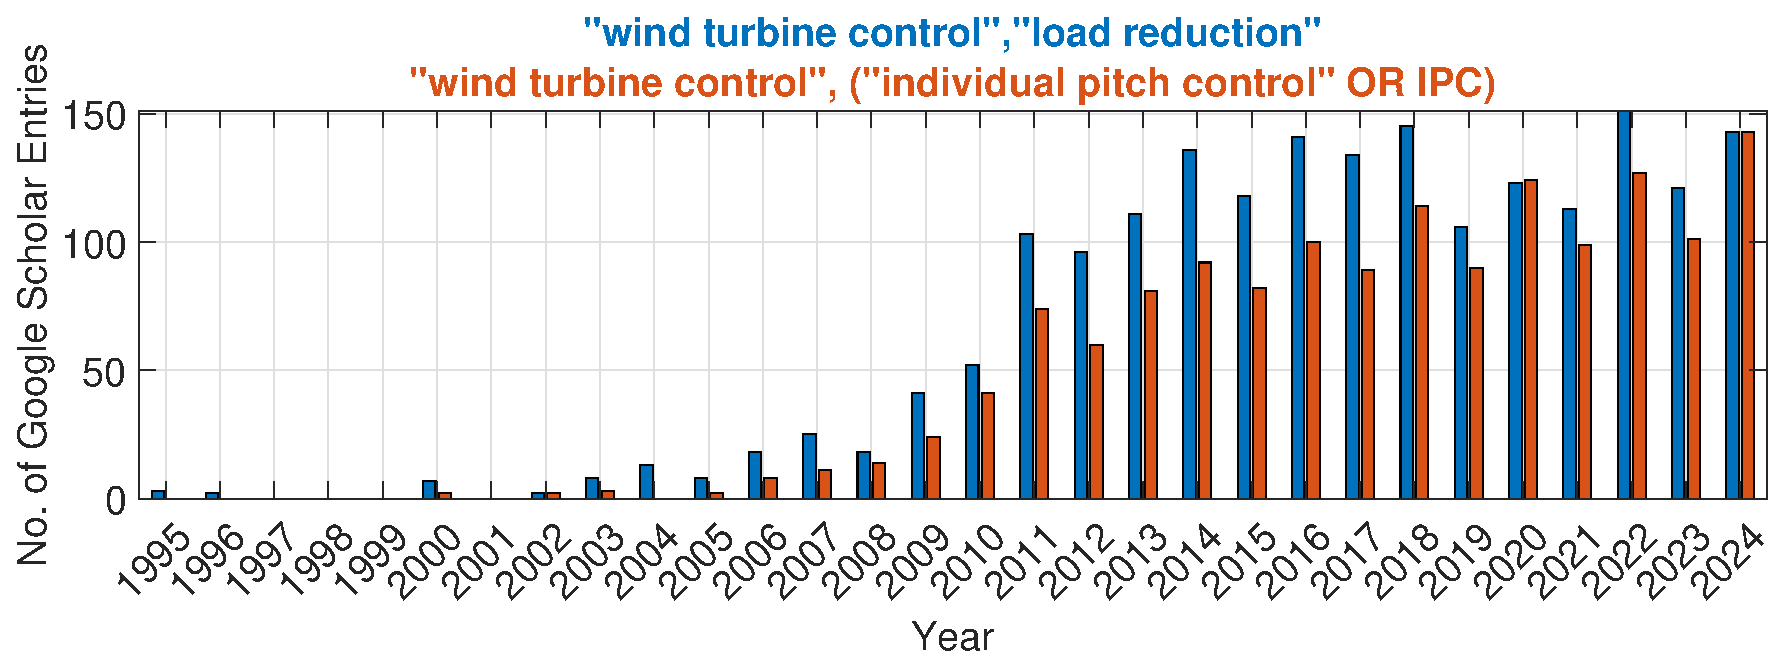
\includegraphics[width=0.8\textwidth]{figures/Figures_ADi/googleWordleWTLoadRedIPC.eps}} \\ %\hfill 
\subfloat[Search term ``model predictive control"]{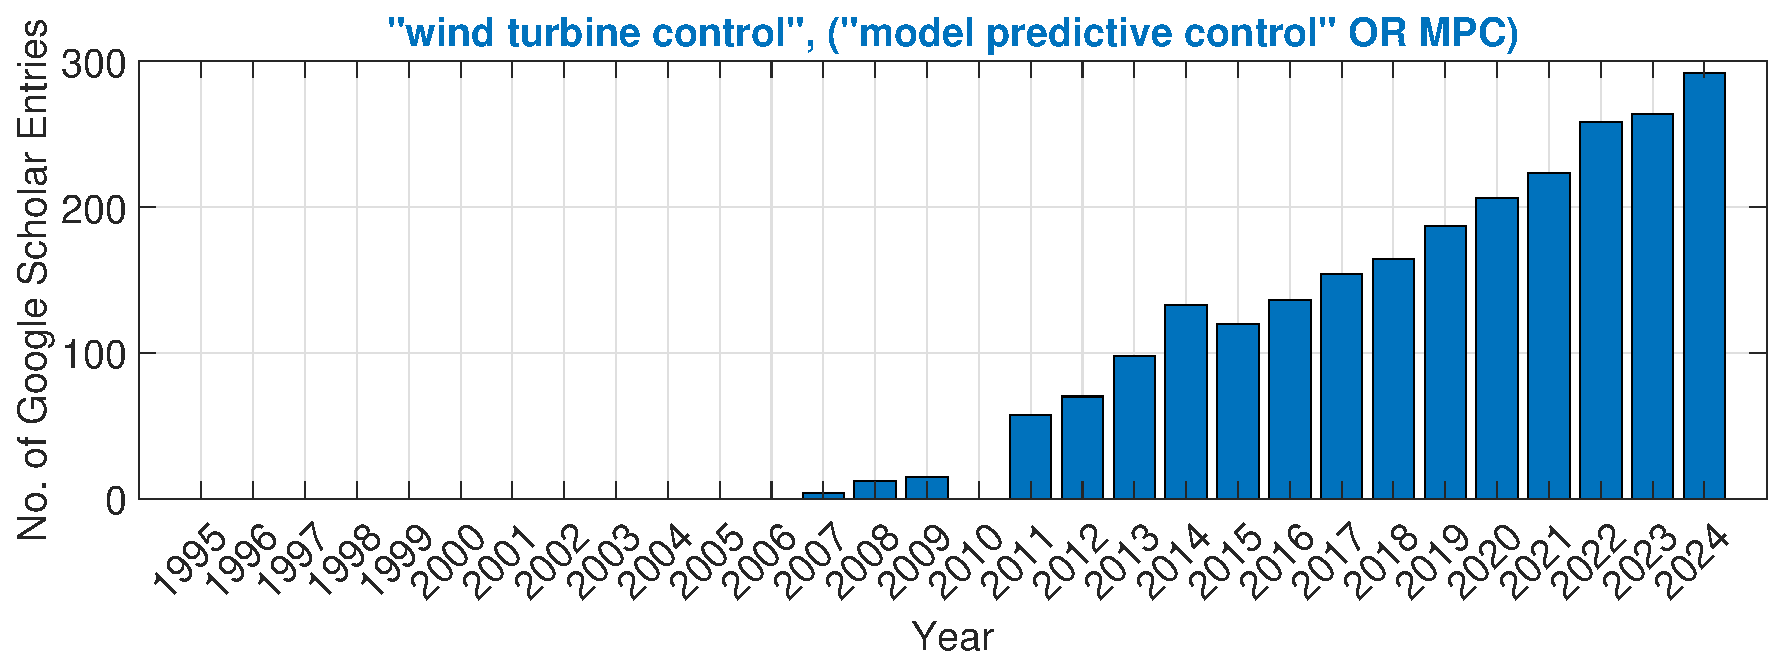
\includegraphics[width=0.8\textwidth]{figures/Figures_ADi/googleWordleWTMPC.eps}} %\hfill
\caption{Number of Google Scholar results by year for the search term ``wind turbine control" and different additional search terms}
\label{fig01:WTstatistics}
\end{figure}

\begin{figure} [h]
\center
\subfloat[Search terms ``axial induction control" and ``wake redirection control"]{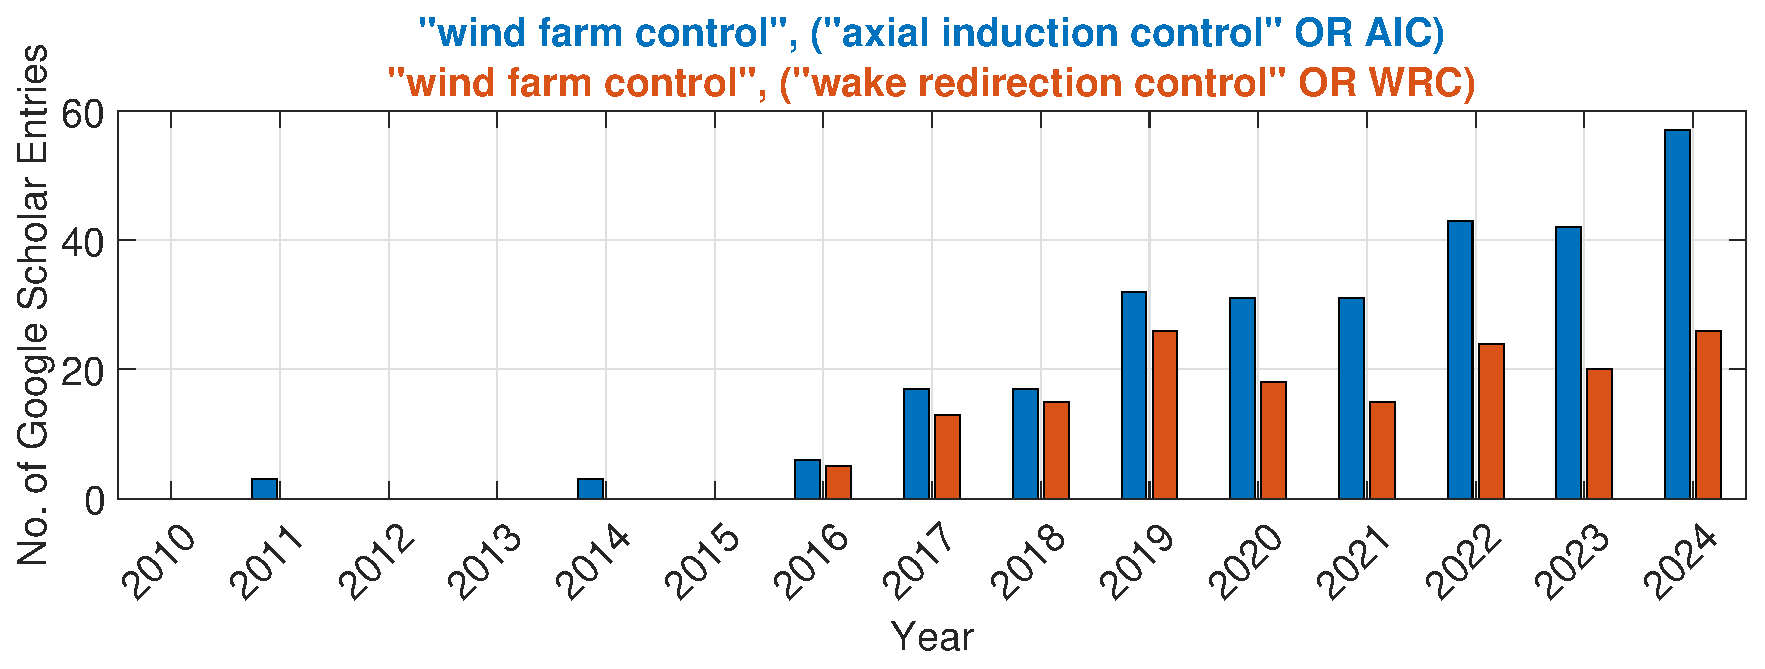
\includegraphics[width=0.78\textwidth]{figures/Figures_ADi/googleWordleWFAICWRC.eps}}\\
\subfloat[Search term ``Koopman"]{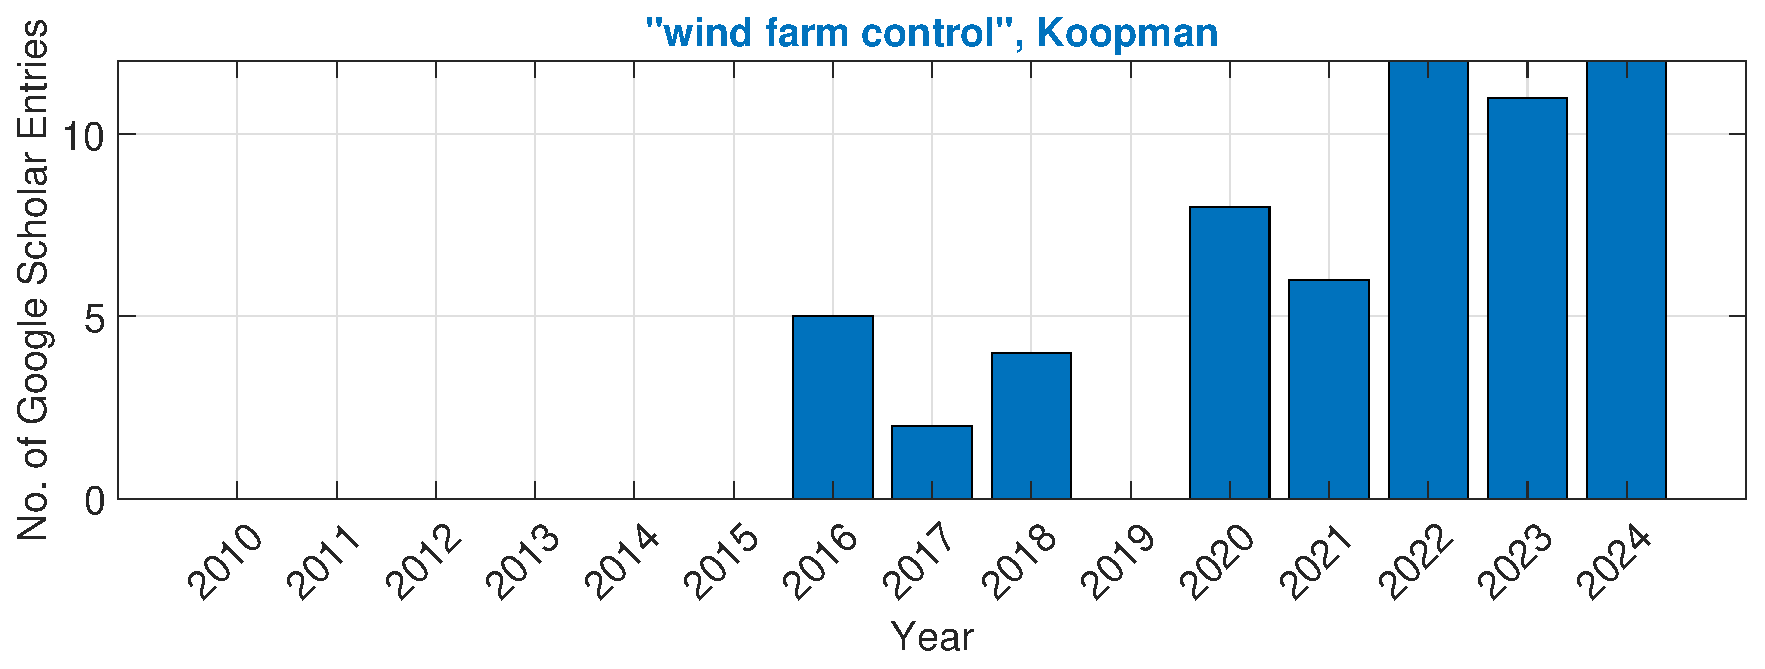
\includegraphics[width=0.78\textwidth]{figures/Figures_ADi/googleWordleWFKoopman.eps}}\hfill
\caption{Number of Google Scholar results by year for the search term ``wind farm control" and different additional search terms }
\label{fig01:WFstatistics}
\end{figure}

Figure~\ref{fig01:WTstatistics}(a) shows a significant increase in the number of published studies over the past approximately fifteen years and a continuously high number, exceeding 100 publications each year, after 2021 for both search terms ``load reduction" and ``individual pitch control". Figure~\ref{fig01:WTstatistics}(b) shows a nearly exponential increase in publication number for MPC and wind turbine control, with more than 200 publications found on Google Scholar each year after 2020.  
%
But while there is extensive literature on load reduction of wind turbines, both via IPC, and MPC, relatively few works explicitly examined quasi-Linear Parameter-Varying (qLPV) MPC, referred to as qLMPC in this thesis. In \cite{Bianchi2007}, modeling wind turbines as qLPV is described, though not within an MPC scheme as in this thesis, but within an $H_{\infty}$ control approach. In \cite{kumar2010FeedbackLinLQR} a nonlinear turbine model is derived and a feedback linearization controller is compared to a Linear Quadratic Regulator (LQR), showing better performance around rated wind speed. The first work to suggest explicitly using the qLMPC introduced in \cite{cisneros2016efficient} for wind turbine control is \cite{mulders2020preventing}, where it is used to derive optimal torque control for tower load reduction as a Single-Input Single-Output (SISO) scheme. This work was followed by a study leveraging a Kalman filter to estimate unmeasurable periodic side-to-side loads in wind turbines, addressing fatigue challenges in tall, slender towers \cite{pamososuryo2022loadestimation}. In \cite{pamososuryo2022individual,pamososuryo2023convex} a convex economic MPC is developed for IPC to actively damp side-to-side tower motion. As load reduction schemes such as IPC require higher actuator activity, actuator constraints become essential in predictive IPC; \cite{petrovic2021mpc} show that their direct inclusion leads to a nonconvex problem and propose a modification of the constraints that preserves convexity. In \cite{feng2022economic} an economic MPC is used to reduce the load distributed over the turbine tower. Recently, the application of velocity-based qLMPC, an algorithm published in \cite{cisneros2020velocity} for reduction of side-to-side tower motion was investigated in \cite{fonseca2024windTurbineSideSide}. In parallel, IPC has been applied in various studies to enable blade root moment reduction: Promising simulation results exist with different control algorithms, e.g., Proportional-Integral-Derivative (PID) \cite{hoffmann2018load}, Linear Quadratic Gaussian (LQG) \cite{selvam2009feedback}, and MPC schemes \cite{petrovic2021mpc}. Field tests confirm the potential of IPC, see \cite{ossmann2021field} and \cite{bossanyi2012advanced}. Recently, TEFs for wind turbines have been suggested for blade root load reductions in \cite{zhang2015parameter} and \cite{bergami2017highfidelity}. As TEFs add an additional degree of freedom to the wind turbines' actuation, there are also studies combining the two methods: In \cite{wilson2009combined}, the standard deviation of blade root flapwise bending moments is reduced up to 32\% for two wind test cases with turbulence class A, at 16\,m/s and 20\,m/s mean wind speed. Turbulence class A at 18\,m/s mean wind speed is used in \cite{henriksen2013model} to investigate the trade-off between load reduction and actuator activity. In \cite{he2018combined}, the blade root flapwise moments and blade tip out-of-plane deflection are both reduced by over 50\%, while also decreasing tower moments for a wind test case of turbulence class B at 20\,m/s. In Chapter~\ref{sec:WindTurbineqLPVModels} of this thesis the design of two qLPV models, one modeling the tower and rotor dynamics as proposed in the previously cited studies and one additionally including blade and generator dynamics as suggested in \cite{Bianchi2007} is presented. In Chapter~\ref{sec:Application to Wind Turbine Control4} the implementation of a velocity-based qLMPC controller is discussed, with a focus on power reference tracking and fore-aft tower motion reduction. This is followed by the design and evaluation of an IPC controller and a combined IPC-TEFC control strategy, which are directly compared to the qLMPC scheme across multiple performance criteria.

Similarly to wind turbine control, Figure~\ref{fig01:WFstatistics}\,(a) shows that for the last ten years wind farm control is a widely studied subject, but that the number of studies leveraging Koopman theory is more limited, see Figure~\ref{fig01:WFstatistics}\,(b). The survey paper \cite{houck2022review} categorizes wake management into AIC, WRC, a combination of WRC and AIC (WRC-AIC), and active wake control. Currently, WRC, which uses yaw to redirect wakes, is the most frequently investigated technique and likely to achieve broader industrial application. However, applying WRC to real wind turbines will require combining it with thrust control via power control for below-rated wind speeds and pitch control for above-rated wind speeds.

Of the eight papers mentioned in \cite{houck2022review} to use combined WRC-AIC, \cite{jimenez2010application} investigates the wake centerline deflection and spread in simulations and \cite{castillo2020wind} in wind tunnel tests. In \cite{bossanyi2018combining} an increase in production and decreased loads, both in the lower one-digit percentage range, is demonstrated in simulations. A lower two-digit percentage increase in power is reported in \cite{cossu2020wake}, based similarly on simulations. In \cite{fleming2016computational} it is concluded that combined WRC-AIC is the control technique resulting in the lowest grid reference tracking error. In the three papers, \cite{park2013wind}, \cite{park2015cooperative}, and \cite{en10070852}, the authors use different, purely data-driven techniques to optimize a combination of induction and yaw control. The advantage of combined WRC-AIC is summarized in \cite{houck2022review} by noting that lowering the thrust of the upstream, misaligned turbine may provide the optimal balance of power increase and load reduction, if wake steering is insufficient to steer a wake completely away from a downstream turbine. But it is mentioned that combined WRC-AIC still requires prior optimizations or real-time computing to implement in the field. However, with a data-driven technique like Koopman MPC a real-time controller can be implemented for wind farms. 

The idea of using the Koopman matrix, a linear approximation of the Koopman operator, to model wind flow and wakes in a wind farm was first suggested in \cite{annoni2016wind} and extended to farm control via AIC in \cite{annoni2016sparsity}. The potential of Dynamic Mode Decomposition (DMD) for wake models was also pointed out in \cite{proctor2016including}, which provides a comparison between DMD and the proper orthogonal decomposition for fluid dynamics modeling. In \cite{munters2017optimal} an MPC is set up with the wind farm dynamics modeled as Large Eddy Simulation (LES) and hence based on NSE and in \cite{munters2018data} the idea of using Koopman to model LES is discussed. In \cite{debnath2017towards} the structure of a wake, simulated via LES, is analyzed. Based on their previous work, it is discussed in \cite{annoni2018sparse} how lidar sensors are to be placed in wind farms to extract a maximum amount of information. In \cite{ali2020data} the varying flow velocities over the blade span are modeled with a linear model derived via Extended DMD (EDMD), taking the forces acting on the rotor excited by the control inputs into account. \cite{chen2020data} discusses using DMD to model the wake flow dynamics. A proof-of-concept for Koopman matrices derived via Extended Input-Output DMD (EIODMD), with the resulting linear state-space models used as basis for MPC, is given in \cite{Cassamo.2020}, which investigates AIC, and in \cite{cassamo2021model} for WRC. An adaptive data-driven MPC algorithm is presented in \cite{cisneros2020data,calderon2021koopman}, and enhanced with a matrix forgetting factor in \cite{calderon2023data}. In Chapter~\ref{sec:ApplicationtoWindFarmControl} of this thesis the application of Koopman MPC to AIC as well as a combination of AIC and WRC is discussed.

\section{Main Contributions}
This section outlines the primary contributions of this thesis in the field of wind turbine and farm control. The research focuses on the integration of novel physics-based and data-driven MPC techniques to optimize wind turbine and farm performance. In all contributions, care was taken to make the algorithms real-time capable, with convergence rates considerably below the 10\,ms sampling time of wind turbine controllers, and to only use measurement information that can realistically be expected to be available during the operation of a real wind turbine. Although the applicability of these algorithms remains at the proof-of-concept stage, they could be applied to wind turbine control with relatively little modification, assuming the necessary sensors and actuators are available. 

The first contribution of this thesis is the development of a real-time capable, velocity-based qLMPC for wind turbine control across the entire operating range. Leveraging Lagrange's equations, a first-principles model incorporating the physics, mechanics, and aerodynamics of the wind turbine was formulated. This model was then utilized in an MPC framework, reformulated as a Quadratic Programming (QP) problem to achieve real-time convergence within millisecond timescales. This work was published in \cite{dittmer2021velocity}.
%
Furthermore, the development and rigorous verification of an AALC system integrating IPC with TEFC is presented. While previous studies had suggested the potential of combining IPC and TEF for wind turbine control, our study, published in \cite{dittmer2024combined}, was the first to rigorously demonstrate the effectiveness of this approach across a wide range of wind speeds. The research evaluated the FAST turbine model extended  with TEFs, using a training dataset and two independent verification datasets, to ensure a comprehensive performance assessment. The results confirmed a significant reduction in blade root out-of-plane moments and tower loads.

The second contribution is the development of an adaptive Koopman MPC framework for wind farm control, marking the first time this efficient update mechanism has been applied in wind farm control simulation. Inspired by the NSE governing turbine interaction, this approach leverages Koopman lifting functions to construct a Koopman matrix for predicting wake interactions and effective wind speed. Computational efficiency is achieved by updating the Koopman matrix only when discrepancies between past predicted and actual wind data are detected. This work builds upon prior research on qLMPC for wind farm control, enhancing its applicability by highlighting its potential to adapt to sudden changes in operation. The findings were published in \cite{dittmer2022data}, extending our earlier work on non-adaptive MPC \cite{sharan2022Koopman}.

Additionally, a data-driven Koopman MPC approach for combined thrust and yaw control in wind farms is demonstrated. Combining thrust and yaw control was motivated by the fact that, due to the slowness of yaw movements, practical implementations of WRC must be combined with pitch and torque control for dynamic load management and efficient power regulation. This combination is driven by the superior power yields achievable with WRC compared to AIC. By incorporating WRC-AIC into the previous AIC framework, this approach achieved a roughly 10\% increase in power output under steady-state conditions and enabled the system to follow grid power references with higher power demands. This data-driven approach directly estimates farm power using a linear system based on the Koopman matrix, eliminating the need for detailed wake modeling. The Koopman MPC framework, presented in \cite{dittmer2023koopman}, demonstrates promising results in achieving reference tracking at reduced actuator activity.

The effectiveness of the proposed MPC controllers is validated through comparative analyses against non-predictive schemes and baseline MPC approaches. Results indicate improvements in power tracking, load reduction, and control quality. Additionally, the wind farm Koopman MPC demonstrates performance with reduced measurement requirements, offering practical advantages over solutions presented in previous studies.

\section{Thesis Structure}
This thesis is organized as follows: Chapter \ref{sec:Background} provides a comprehensive review of the physics of wind, wind turbine and wind farm dynamics, and their control. The fundamental ideas of qLPV models and MPC are presented. The chapter also introduces the Koopman operator and DMD.

Chapter~\ref{sec:WindTurbineqLPVModels} focuses on the development of a qLPV wind turbine model. Two models are derived: one modeling the rotor speed and tower movements only, and one, using Lagrange's equations, modeling additionally blade movements and generator speed. The quality of the two qLPV models is verified across the entire turbine operating range in both frequency and time domains using the software FAST.

Chapter~\ref{sec:Application to Wind Turbine Control4} presents the work on wind turbine control, encompassing both the velocity-based qLMPC framework and the AALC system integrating IPC with TEFC. The qLMPC framework is discussed in terms of its reformulation as a  QP problem for real-time implementation. Its performance is evaluated for power tracking and load reduction, with comparative analyses against baseline control methods. The chapter also discusses the effectiveness for reducing blade root and tower loads over a wide range of wind speeds with the IPC-TEFC approach.   

Chapter~\ref{sec:ApplicationtoWindFarmControl} describes Koopman MPC for wind farm control: an adaptive Koopman MPC using thrust control and a Koopman MPC for combined thrust and yaw control. The software WFSim and enhancements necessary to evaluate the presented algorithms are discussed. The adaptive Koopman MPC leverages efficient update mechanisms to deal with abrupt changes, while the combined thrust and yaw approach integrates WRC with AIC to increase power yield. The chapter evaluates the proposed methods for power output improvement, grid reference tracking, and actuator activity reduction.

Chapter~\ref{Conclusions} summarizes the main contributions and findings of the thesis 
and discusses the practical implications of the proposed control strategies. It provides 
a discussion of existing challenges, concretely relating to sensor 
integration, actuator degradation, and validation in higher-fidelity simulation 
environments. Finally, it outlines directions for future research, including the 
extension to more realistic wind conditions and the use of Neural Network-based 
lifting functions as an alternative to physically motivated lifting functions.
    \chapter{Background} \label{sec:Background}

Simulations can only evaluate the effects of different control algorithms meaningfully if the underlying simulation models reasonably resemble reality. This background chapter provides an overview of the physical models used to describe the behavior of wind in Section~\ref{sec:Wind} and wind turbines in Section~\ref{sec:WindTurbines}. The interaction of wind turbines in farms via wake effects is described in Section~\ref{sec:WakeModels}. Baseline control schemes for both wind turbines and wind farms, against which the designs in this thesis are evaluated, are also presented in these sections. Section~\ref{sec:Control-Theoretic Background} presents the mathematical foundations of the two modeling frameworks used in this thesis, i.e., qLPV for wind turbines and Koopman for wind farms, followed by the MPC framework applied to both.

\section{Wind} \label{sec:Wind}

While wind, unlike conventional energy sources, cannot be controlled, its dynamics are well studied and understood. Detailed information on the aerodynamics of wind and wind turbines can be found, for example, in~\cite{hansen2015aerodynamics} and~\cite{hau20084}. The following section provides an overview of the related chapter in~\cite{Bianchi2007}, which summarizes the physics of wind.

Standardized wind models from the International Electrotechnical Commission (IEC) are used for testing and for the certification of controllers. The economic viability of a wind energy project, and hence decisions that need to be made prior to construction, such as the number and exact location of turbines in a farm or the turbine type, depend on the temporal and spatial wind distribution at the investigated site. These wind measurements also influence the choice of IEC wind models used for controller synthesis and closed-loop controller testing.
%
Wind is generated by temperature differences caused by uneven solar heating of the atmosphere. Wind can be classified into large-scale airflows, called geostrophic wind, which occurs in all layers of the atmosphere, and local wind. Local wind flows develop in the surface layer of the atmosphere, which extends up to a height of 100\,m and is therefore affected by geographical features and surface topography.

The kinetic energy frequency distribution of wind speeds follows a typical pattern, called the van der Hoven spectrum. The spectrum has two peaks, one at approximately 0.01 cycles per hour, representing a four-day cycle, and another at around 50 cycles per hour, roughly corresponding to one-minute cycles. These peaks are separated by an energy gap, indicating lower energy content in wind speeds with periods between ten minutes and two hours. The low-frequency side of the spectrum is associated with geostrophic wind, while the high-frequency side represents local wind speeds, including turbulence. The aeroelastic forces that turbines are subjected to over their lifespan are caused by mean wind speeds, i.e., constant stationary air movement, and stochastic turbulence. Hence, ten-minute time series with different mean values and different turbulence classes are traditionally used for controller testing and load analysis in wind energy applications.

The quasi-steady mean wind speed $\bar{V}$ at a site is the most important factor influencing the potential profitability of a wind energy project and the selection of appropriate wind turbines to maximize the Annual Energy Production (AEP) over the turbines' lifespan. The probability distribution of mean wind speeds is often predicted based on long-term measurements and can typically be approximated by the Weibull distribution:
\begin{equation}
    f_{\text{WB}}(\bar{V}) = \frac{k_{\text{WB}}}{C_{\text{WB}}}\left(\frac{\bar{V}}{C_{\text{WB}}}\right)^{k_{\text{WB}}-1}e^{- (\bar{V}/C_{\text{WB}})^{k_{\text{WB}}}}
\end{equation}
with shape and scale coefficients, $k_{\text{WB}}$ and $C_{\text{WB}}$, respectively, describing the probability of different wind speeds occurring at the site.

Mean wind speed also varies with height above ground level as surface roughness and obstacles affect wind speed through frictional forces. This spatial speed variation is called wind shear and can be described by different models, among them the power law:
\begin{equation}
    \bar{V}(z) =  \bar{V}(z_{\text{ref}})\left(\frac{z} {z_{\text{ref}} }\right)^{\alpha_{\text{shear}}} 
\end{equation}
where $z$ is the height above ground, $z_{\text{ref}}$ is a reference height, often 10\,m, and $\alpha_{\text{shear}}$ is the wind shear exponent. In \cite{Bianchi2007}, values for sand, mown and high grass, and suburban areas are given, varying from 0.10 to 0.32. In this work, the commonly used wind shear exponent $\alpha_{\text{shear}} = 0.2$ is used.

While turbulence has a minor influence on the AEP, it significantly impacts aerodynamic loads and power variance. Power variance is relevant to power quality, as maintaining a smooth power output is important, especially in smaller networks.

Turbulence is stochastically described by its power spectrum. Two widely used models are the von K\'arm\'an and Kaimal spectra:
\begin{equation}
    \Phi_{\text{K\'arm\'an}}(\omega) = \frac{K_V}{(1 +(\omega T_V)^2)^{5/6}} \quad \text{and} \quad
    \Phi_{\text{Kaimal}}(\omega) = \frac{K_V}{(1 +\omega T_V)^{5/3}},
\end{equation}
where $\omega$ is the angular frequency, $T_V$ is a time constant whose inverse determines the turbulence bandwidth, and $K_V$ scales the turbulence power. The two parameters take different values in the two models. For the von K\'arm\'an spectrum, they are approximated as~\cite{Bianchi2007}
\begin{equation}
    K_V = 0.475 I_v^2 \frac{L_v}{\bar{V}(z)} \quad \text{and} \quad T_V = \frac{L_v}{\bar{V}(z)},
\end{equation}
and for the Kaimal spectrum, following IEC~61400-1~\cite{IEC61400-1}, as
\begin{equation}
    K_V = \frac{2}{\pi} I_v^2 \frac{L_v}{\bar{V}(z)} \quad \text{and} \quad T_V = \frac{3}{\pi}\frac{L_v}{\bar{V}(z)},
\end{equation}
with the turbulence intensity $I_v$, which represents the ratio of the standard deviation of wind speed fluctuations to the mean wind speed, and the integral length scale $L_v$, which indicates the spatial scale of turbulence. Both spectra are normalized by $\bar{V}^2(z)$, i.e., they describe the fluctuations relative to the mean wind speed; multiplying them by $\bar{V}^2(z)$ yields the spectra of the wind speed fluctuations. Note that $L_v$ is defined differently in the two models. The Kaimal model is used by TurbSim, which generates the turbulent wind fields in FASTTool. Therefore, all turbulent wind test cases presented in this thesis are based on it.


The turbulence intensity, which depends on the height of the turbine and the terrain of a potential site, is an important factor in site selection. Higher turbulence intensity leads to increased aerodynamic loads on turbine structures, influencing the durability and performance of wind turbines.

\section{Wind Turbines} \label{sec:WindTurbines}

Wind turbines extract kinetic energy from the wind and convert it into other energy forms, most often electricity. In this section, commonly used mathematical representations based on the physics governing wind turbine behavior are provided, and a state-of-the-art control scheme for modern wind turbines is discussed.

\subsection{Wind Turbine Simulation Models}\label{windTurbineModel}
Depending on the application, different models are used to describe the physical effects of a wind turbine. In their simplest form, wind turbines can be modeled as an energy sink using the actuator disk model, which is the model used in the Wind Farm Simulator (WFSim)~\cite{boersma2018control}. Alternatively, the Blade Element Momentum (BEM) model can be used directly, as in FAST~\cite{jonkman2005fast}, or via lookup tables for rotor thrust and torque to include the effect of varying rotor speed and pitch angles on the forces and moments. All models in this thesis are parameterized for the 5\,MW reference turbine of the National Renewable Energy Laboratory (NREL), the NREL 5MW, with its physical parameters listed in Table~\ref{table:1}.

\subsubsection{Actuator Disk Model}
The amount of energy extracted from the wind depends on the wind speed difference between the wind in front of the turbine and the wind behind it. Figure~\ref{fig:ActDiscModel} visualizes the airflow through a rotor disk, showing the wind speeds, pressures, and corresponding areas of the airflow far ahead and far behind the turbine, as well as at the rotor.
%
\begin{figure}[ht]
    \centering
    \includegraphics[width=0.76\textwidth,trim={0cm 0.3cm 3.5cm 0.4cm},clip]{figures/figuresBlockDiagram_IFAC23/testTurbineBetz.pdf}
    \caption{Airflow through a wind turbine, modeled as an actuator disk, adapted from \cite{Bianchi2007}.}
    \label{fig:ActDiscModel}
\end{figure}
%
The available amount of wind power $P_w$ and the amount of power $P_r$ extracted by the turbine rotor at the rotor area $A_r$ are given by:
\begin{align} \label{eq:PwPt}
    P_w = \frac{1}{2} \rho_a A_r V_{\infty}^3,\quad\text{and} \quad  P_r = c_P P_w,
\end{align}
where $\rho_a$ is the air density, $V_{\infty}$ is the freestream wind speed, and $c_P$ is the power coefficient. The mean wind speed at the rotor disk $V_r$, also called the effective wind speed, is related to the freestream wind speed $V_{\infty}$ by:
\begin{align} \label{eq:ainduct}
    V_r = (1-a)V_{\infty},
\end{align}
where $a$ is the axial induction factor. The thrust $F_{T,r}$ acting on the turbine can be calculated from the pressure difference $\Delta p_r$ at the rotor disk. This pressure difference depends on the freestream wind and the wind speed $V_{\text{-}\infty}$ far behind the turbine, leveraging Bernoulli's equation:
\begin{equation}\label{eq:pVBernoulli}
    \Delta p_r = \frac{1}{2} \rho_a(V_{\infty}^2  - V_{\text{-}\infty}^2 ).
\end{equation}
The thrust $F_{T,r}$ can be determined either from the rotor area and the pressure difference in Equation~\eqref{eq:pVBernoulli}:
\begin{align} \label{eq:Ft1}
    F_{T,r} = A_r \Delta p_r =  \frac{1}{2} \rho_a A_r (V_{\infty}^2  - V_{\text{-}\infty}^2 ) 
\end{align}
or alternatively as the product of the air mass flow through the rotor area $\dot{m}_a$ and the wind speed difference:
\begin{align} \label{eq:Ft}
    F_{T,r} =  \dot{m}_a  (V_{\infty} - V_{\text{-}\infty}) = \rho_a A_r V_r (V_{\infty} - V_{\text{-}\infty}).  
\end{align}
From Equations \eqref{eq:ainduct}, \eqref{eq:Ft1}, and \eqref{eq:Ft}, the thrust of the rotor can be calculated as:
\begin{align} \label{eq:Ftall}
    F_{T,r} = 2a(1-a) \rho_a A_r V_{\infty}^2.
\end{align}
Combining Equations \eqref{eq:PwPt} to \eqref{eq:Ft} and using the fact that $P_r = F_{T,r} V_r$, the relationship between the axial induction factor $a$ and the power coefficient $c_P$ is:
\begin{equation}\label{eq:cpFromA}
    c_P(a) = 4a(1-a)^2,
\end{equation}
with the axial induction factor maximizing power yield given by $a^* = 1/3$ and the maximum $c_P(a^*) = 16/27$, known as the Betz limit. The wind speed difference and, consequently, the amount of power extracted from the wind, are influenced in real turbines by changing the generator torque and adjusting the blade pitch angle, both of which affect the turbine's rotor speed.

\subsubsection{Blade Element Momentum Theory}
The actuator disk model is a significantly simplified representation of the physics of a wind energy conversion system (WECS). Wind turbines consist of an aerodynamic subsystem, a flexible drivetrain, and a power generator, with the aerodynamic subsystem responsible for converting the available kinetic energy of the wind into useful mechanical energy through the rotor blades \cite{SaMuAlBe18}. 

Figure~\ref{figBEMModel} visualizes the local flow conditions and force components at a blade element, as used in BEM theory. In this model, the rotor is divided into small segments, each treated as an independent airfoil.
\begin{figure}[ht] %  %The Blade Element Momentum (BEM) model, as visualized in Figure \ref{figBEMModel}, refines the actuator disk model by incorporating the detailed aerodynamic behavior of individual rotor blades. 
    \centering
    \includegraphics[width=0.96\textwidth,trim={0cm 0cm 0cm 0cm},clip]{figures/figuresBlockDiagram_IFAC23/turbineAirfoilBem.pdf}
    \caption{Local airflow and forces on a blade element of width $dr$ at radial position $r$, based on \cite{hansen2015aerodynamics} and adapted from \cite{weiss2016regelungstechnische}.} 
    \label{figBEMModel}
\end{figure}

BEM theory combines the principles of blade element theory, which calculates the forces on each blade segment based on local airflow conditions, and momentum theory, which models the changes in wind velocity and pressure as air passes through the rotor disk. The lift and drag forces $dF_L$ and $dF_D$ on each blade element located at a radial position $r$ are determined by the angle of attack $\alpha$, the pitch angle $\beta$, the local airspeed $V_\text{inflow}$, the rotational speed of the rotor $\omega_r$, and the tangential flow induction factor $a^{\prime}$. The wind speed component $V_r$ is calculated from the freestream wind speed $V_{\infty}$ and the axial induction factor $a$ as described in Equation~\eqref{eq:ainduct}. The forces $dF_L$ and $dF_D$ are used to determine the thrust $F_{T,r}$ and torque $T_r$ generated by the rotor. 

The lift and drag forces, which act perpendicular and parallel to the inflow of a blade section with chord $c$ and width $dr$, are:
\begin{align} \label{eq:dFldFd}
    dF_L &= \frac{1}{2} \rho_a V^2_{\text{inflow}} c_L(\alpha)cdr,\\
    dF_D &= \frac{1}{2} \rho_a V^2_{\text{inflow}} c_D(\alpha)cdr,
\end{align}
where the lift and drag coefficients $c_L$ and $c_D$ depend on the angle of attack $\alpha$. As shown in Figure \ref{figBEMModel}, the angle $\phi$ between the local flow direction and the rotor plane is the sum of the angle of attack $\alpha$, the pitch angle $\beta$, and the local twist angle of the blade. The thrust and torque of each segment can be calculated as:
\begin{align} \label{eq:dFTrdTr}
    dF_{T,r} &= dF_{L}\cos\phi + dF_D \sin\phi,\\
    dT_r &= (dF_{L} \sin \phi - dF_D \cos\phi) r.
\end{align}
The relative wind speed at the blade depends on its perpendicular and tangential components:
\begin{align} \label{eq:dFTrdTr1}
    V_{\text{inflow}} = V_{\infty}\sqrt{(1-a)^2 + \left(\frac{\omega_{r}r}{ V_{\infty}}(1+a^{\prime})\right)^2}\text{ and } \tan \phi = \frac{V_{\infty}}{\omega_r r} \frac{1-a}{1+a^{\prime}}.
\end{align} % where $a$ is the axial induction factor and $a^{\prime}$ is the tangential induction factor. 
The two induction factors $a$ and $a^{\prime}$ can be calculated if the blade element properties $c_L(\alpha)$, $c_D(\alpha)$, $r$, and $dr$ are known, as well as the current values of variables influencing the local force. These variables include $\rho_a$, $V_{\infty}$, $\omega_r$, and $\beta$. The BEM theory, as implemented in FAST, assumes steady, incompressible flow and calculates the rotor's performance iteratively using Equations \eqref{eq:pVBernoulli} to \eqref{eq:dFTrdTr1}. Thus, the interaction between the blade elements and the wind is considered in computing the forces, moments, and movements of the WECS. This iterative process is used to simulate performance under different wind conditions. The movement of the blades and tower is calculated in FAST using a linear modal representation, which exploits the fact that the deflections are relatively small.

The wind turbine modeling approaches discussed in this section account for the influence of wind-speed variations on turbine operation. However, the instantaneous power extracted from the wind depends not only on the available wind speed but also on the turbine’s control inputs, i.e., generator torque and blade pitch angle. The next subsection provides an overview of state-of-the-art wind turbine control strategies.


\subsection{Wind Turbine Control} \label{sec:WindTurbineControl}

All modern wind turbines use a control system to regulate rotor speed. The control settings of a wind turbine are determined by the energy available in the wind as well as economic considerations. Figure \ref{fig:WindREgion} visualizes the power output at different wind speeds.

\begin{figure}[ht]
    \centering
    \includegraphics[width=0.8\textwidth,trim={0.5cm 0.4cm 0.0cm 0.3cm},clip]{figures/Figures_ADi/windRegionen.pdf}
    \caption{Power output curve in Regions I to IV, based on the control region definitions for the NREL 5MW reference turbine in \cite{jonkman2009definition}.}\label{fig:WindREgion}
\end{figure}

At very low wind speeds, below the so-called cut-in wind speed $V_{\text{cut-in}}$, the power that could be produced would not cover the operating costs. The wind speed region up to the cut-in wind speed is referred to as Region I. The wind speed region between the cut-in wind speed and the rated wind speed $V_{\text{rated}}$ of a turbine, i.e., the wind speed corresponding to the rated power of the turbine, is called Region~II. 

For wind speeds above the rated wind speed, the blades are pitched to keep the power output constant and to reduce excessive mechanical loads that would otherwise shorten the turbine's operational lifespan. At very high wind speeds, above the cut-out wind speed $V_{\text{cut-out}}$, the turbine stops operating. Region III is the wind speed range between rated and cut-out wind speed, while Region IV refers to wind speeds above the cut-out wind speed.

At each wind speed between the cut-in and cut-out wind speeds, a control system ensures the most profitable power output by regulating the generator torque $T_g$ and the blade pitch angle $\beta$. Generator torque is used to maximize power yield at wind speeds in Region~II. The blade pitch is used to maintain a constant power output at rated power for wind speeds above the rated wind speed and below the cut-out wind speed in Region~III. The power controller receives feedback from the generator rotational speed $\omega_g$ across all operating regions. 

In this work, the power controller available within TU Delft's FASTTool \cite{mulders2020wind} is used as a baseline, see Table~\ref{table:pitch_ctrl} for its parameters. FASTTool features a MATLAB graphical user interface for setting up simulations and tuning control parameters for an underlying Simulink model, which represents the dynamics of the NREL 5MW turbine. The underlying physical principles are detailed in \cite{jonkman2009definition}. 


\subsubsection{Generator Torque Control}

In Regions I\,1/2 and II, the generator torque is governed by the so-called $k\omega^2$ control law, which is implemented as a tabulated function of the generator speed $\omega_g$. In Region~I\,1/2, the start-up phase just above the cut-in wind speed, see Figure~\ref{fig:WindREgion}, a multiplication factor is applied to compute the reference generator torque $T_{g,\text{ref}}$. In most of Region~II, an optimal factor $K^*$ is multiplied by the square of the rotational speed.

The upper portion of Region II, just below the rated wind speed, is referred to as Region~II\,1/2. In this transition zone, a smooth linear interpolation is applied up to the rated rotational speed. This ensures a seamless transition within Region~II while also maintaining compliance with noise emission regulations and limiting excessive mechanical loads. These controller settings, originally defined in \cite{jonkman2009definition}, have been implemented without modifications in \cite{mulders2020wind}, preserving both the algorithmic structure and parameter values.

\subsubsection{Blade Pitch Control} 

In Region III, the collective pitch control strategy relies on a scheduled PI controller, where the proportional and integral gains, $K_P(\omega_g)$ and $K_I(\omega_g)$, are dynamically adjusted based on the generator speed. This adaptive gain scheduling enhances the tracking of the maximum allowable rotor speed. The gain values used in this implementation remain unchanged from those provided in the original FASTTool repository.

The derivation of these gains follows from \cite{jonkman2009definition}. The difference between the aerodynamic torque $T_r$ and the generator torque $T_g$, with the latter multiplied by the gear ratio $N_g$, is equal to the product of drivetrain inertia $J_{s}$ and the rotor acceleration $\Delta \dot{\omega}_r$:

\begin{equation} \label{eq:Tr1_background}
    T_r -N_g T_g = (J_r + N_g^2 J_g) \frac{d}{dt}(\omega_{\text{rated}} + \Delta \omega_r) = J_{s} \Delta \dot{\omega}_r,
\end{equation}
where $J_r$ and $J_g$ are the rotor and generator inertias, respectively. The aerodynamic and generator torques, derived from the rated power $P_{\text{rated}}$, can be approximated as Taylor series expansions:

\begin{align}
    T_g(\omega_r) &= \frac{P_{\text{rated}}}{N_g \omega_r} \approx  \frac{P_{\text{rated}}}{N_g \omega_{\text{rated}}} - \frac{P_{\text{rated}}}{N_g\omega_{\text{rated}}^2} \Delta \omega_r,  \label{eq:Tg}\\
    T_r(\beta) &= \frac{P(\beta,\omega_r)}{\omega_r}   \approx \frac{P_{\text{rated}}}{\omega_{\text{rated}}} + \frac{1}{\omega_{\text{rated}}}\Big(\frac{\partial P}{\partial \beta}\Big) \Delta \beta.  \label{eq:Tr_background}
\end{align}
%
The desired change in pitch angle, $\Delta \beta$, is calculated based on the rotor speed deviation $\Delta \omega_r$ using a PID controller:

\begin{align} \label{eq:PID}
    \Delta \beta = K_P N_g \Delta \omega_r + K_I \int_{0}^{t}N_g \Delta \omega_r dt + K_D N_g \Delta \dot{\omega}_r.
\end{align}
%
Substituting Equation~\eqref{eq:PID} into Equation~\eqref{eq:Tr_background} and incorporating the relationships from Equations \eqref{eq:Tr1_background} and \eqref{eq:Tg} leads to the final control formulation with the substitute state $\dot{x} = \Delta \omega_r$ and derivative $\mathcal{P}_\beta = \left( -\frac{\partial P}{\partial \beta} \right)$:

\begin{equation}\label{eq:PID2} 
    \underbrace{\left[ J_{s} + \frac{\mathcal{P}_\beta}{\omega_{\text{rated}}} N_{g} K_D \right]}_{M_{x}} \ddot{x}(t) 
    + \underbrace{\left[ \frac{\mathcal{P}_\beta}{\omega_{\text{rated}}} N_{g} K_P - \frac{P_{\text{rated}}}{\omega_{\text{rated}}^2} \right]}_{C_{x}} \dot{x} (t)
    + \underbrace{\left[ \frac{\mathcal{P}_\beta}{\omega_{\text{rated}}} N_{g} K_I \right]}_{K_{x}} x(t) = 0.
\end{equation}
%
The PID gains are determined to achieve the desired natural frequency and damping ratio, which, in turn, dictate how the mass $M_{x}$, damping $C_{x}$, and spring term $K_{x}$ should be set through the control parameters. The value of  $\mathcal{P}_\beta$, i.e., the sensitivity of the aerodynamic power to the blade pitch, can be calculated for the different operating points and is provided in \cite{jonkman2009definition}. 

In the implementation of \cite{mulders2020wind}, a gain-scheduled PI controller is used by default, with the derivative term set to zero. The controller gains are modified from those originally suggested in \cite{jonkman2009definition}, aiming to achieve a smoother power output. A fixed-gain PI controller is also available in FASTTool, but for this study, the default gain-scheduled PI controller is employed.

\subsubsection{Yaw Control}
Yaw control in modern wind turbines is responsible for aligning the turbine with the wind direction based on wind vane measurements on the nacelle. The wind direction is averaged over time, and yaw adjustments are performed if the averaged yaw misalignment exceeds a predefined threshold. Due to the large structural loads associated with yaw motion, adjustments are made infrequently to ensure the longevity of the yaw system. As a result, yaw control does not directly influence the turbine's power control.

However, in wind farm settings, deliberate yaw misalignment, i.e., intentional yaw offset, has been actively researched over the past decade as a means to mitigate wake effects on downstream turbines. By strategically redirecting the wake, this approach aims to optimize the overall power output of a wind farm rather than maximizing the efficiency of individual turbines.

\subsection{Control Objectives}\label{subsection Control Objectives}
The overall goal of both wind turbine and wind farm control is to minimize the Levelized Cost of Energy (LCoE). This requires balancing the often contradictory objectives of maximizing power yield while minimizing the mechanical Damage Equivalent Loads (DEL) on the tower and blades, as well as reducing actuator energy consumption. Below is a brief overview of load analysis for wind turbine controllers and the objectives for controller evaluation applied in this thesis. Five of the six criteria described below are inspired by the five objectives used in \cite{hoffmann2018load}; the DEL of the tower top fore-aft moment is added. 



\subsubsection{Load Analysis}
Before wind turbine controllers are applied in production, they must be certified based on an extensive load analysis. This analysis uses Design Load Cases (DLCs), which are 22 standard scenarios defined by the IEC~61400-1~\cite{IEC61400-1} and classified into~17 ultimate and~5 fatigue load case scenarios. The wind conditions used in the DLCs depend on the turbine class, which is chosen according to the mean wind speed at the location of the WECS. The average wind speeds for turbine Classes I, II, and III are 10\,m/s, 8.5\,m/s, and 7.5\,m/s, respectively. In addition to the mean wind speed, the turbulence intensity is considered with three different classes. In this work, the reference turbulence intensities of the IEC~61400-1 for Classes A, B, and C are used, i.e., 16\%, 14\%, and 12\%, respectively, as implemented in the \textit{InflowWind.m} file of the FASTTool. These are the expected values at a hub-height wind speed of 15\,m/s. Older editions of the standard and some literature give higher values, e.g., 18\% for Class A and 16\% for Class B \cite{gasch2011wind}. Throughout this thesis, the turbulence classes refer to the values given in the FASTTool.

The ultimate load DLCs are used to verify that a turbine can withstand the maximum load that is statistically likely to occur during its lifetime. Fatigue load analysis is applied to demonstrate that a turbine can endure structural loads over time. For this analysis, closed-loop simulations of 660\,s are conducted using different turbulent wind test cases from the relevant IEC wind classes, with different random seeds for wind initialization. The first 60\,s of simulated data are discarded to avoid introducing initialization artifacts into the analysis, and the remaining 600\,s are used to calculate the DEL. This approach is used in the context of certification to verify the suitability of a control strategy. In this thesis, it is applied for controller testing and performance comparison.


\subsubsection{DEL Criteria $C_{\text{DEL},b}$ and $C_{\text{DEL},t}$}

For the DEL calculation of signals such as blade and tower bending moments, their load cycles are first classified using rainflow counting \cite{matsuishi1968fatigue}. In this thesis, the MATLAB implementation in \textit{rainflow.m} is used to derive the cycle count vector $\bm{l}_D \in \mathbb{R}^{n_l }$ and the corresponding range vector $\bm{R}_{\text{DEL}}\in \mathbb{R}^{n_l }$, i.e., their peak-to-peak amplitudes, for the simulation signal of a bending moment, with $n_l$ as the number of stress levels. 


In a second step, the elements of the vectors $\bm{l}_D$ and $\bm{R}_{\text{DEL}}$ are applied to calculate damage from the moment signals. This is based on Miner’s rule, which calculates damage from stress signals as:
\begin{equation} \label{eq:Miner0}
    D =  \sum_{i=1}^{n_l} D_i = \sum_{i=1}^{n_l} \frac{l_i}{L_i} = 
    \sum_{i=1}^{n_l} \left( \frac{l_i}{L_D} \left(\frac{\sigma_i}{\sigma_D} \right)^m \right)
    = \frac{1}{L_D\sigma_D^m} \sum_{i=1}^{n_l}  \left( l_i \sigma_i^m \right)
\end{equation}
where $D$ represents the damage fraction at a given point in time, with $D = 1$ indicating the end of the remaining useful life. The mean number of cycles to failure is denoted $L_i$, and $l_i$ is the recorded number of cycles at stress level $\sigma_i$. The equation can be reformulated to explicitly account for material properties, where $L_D$ is the number of cycles to failure at the terminal stress amplitude $\sigma_D$, $\sigma_i$ is the actual occurring stress amplitude, and $m$ is the W\"ohler exponent, which depends on the material. In this thesis, the commonly used W\"ohler exponents of $m_{\text{Steel}} = 4$ for the tower and $m_{\text{GFRP}} = 10$ for the blades of the NREL 5MW, which are made of Glass Fiber Reinforced Polymer (GFRP), are used for the evaluation criteria; the optimizations in Chapter~\ref{sec:Application to Wind Turbine Control4} use the exponents~8 and~3 of \cite{dittmer2024combined}.

Leveraging Equation~\eqref{eq:Miner0}, a reference range $R_{\text{DEL},\text{ref}}$ and reference cycle number $l_{\text{ref}}$ are introduced:
\begin{align}
    l_{\text{ref}} R_{\text{DEL},\text{ref}} ^m = \sum_{i=1}^{n_l}  \left(l_i R_{\text{DEL},i}^m \right) \iff R_{\text{DEL},\text{ref}} = \sqrt[m]{\frac{ \sum_{i=1}^{n_l} \left(l_i R_{\text{DEL},i}^m \right)}{l_{\text{ref}}}}.
\end{align}
The reference number of cycles is set to the commonly used value $l_{\text{ref}}=2\cdot10^6$. From the reference range, the DEL over the lifetime can be derived by calculating the reference range for the different wind speed and turbulence scenarios likely to occur and weighting them using Weibull distributions.

In this thesis, the damages of the blade and tower moments are calculated for a closed-loop simulation run with the baseline controller, as described in Section~\ref{sec:WindTurbineControl}. A second simulation with the same wind file is then run with the controller design to be compared with this baseline, e.g., a qLMPC design. The ratios of the damages of the two runs, taken to the power $1/m$, i.e., the ratios of the DELs, form the criteria $C_{\text{DEL},b}$ for the blades, with the damages summed over the three blades, and $C_{\text{DEL},t,\text{Base}}$ and $C_{\text{DEL},t,\text{Top}}$ for the fore-aft moments at the tower base and the tower top. Values below 1 hence indicate a reduction in blade and tower loads, respectively, and are therefore considered an improvement of the closed-loop behavior.


\subsubsection{Power Criteria $C_{\bar{P}}$ and $C_{\delta P}$}
The mean generated power, which should not decrease compared with the baseline controller, and the standard deviation of the generated power are used as performance criteria. Particularly in smaller networks, a power output with a small standard deviation improves grid stability by reducing fluctuations. The criteria $C_{\bar{P}}$ and $C_{\delta P}$ are calculated by normalizing the values obtained from simulations with the controller designs developed in this work by the values obtained from simulations with the baseline controller.

\subsubsection{Actuator Power Criterion $C_{\text{Act}}$}
Actuator movements must be limited to prevent excessive wear of the pitch actuators and avoid unnecessary energy consumption. The actuator power is calculated as the mean absolute product of the pitch rate and the pitching moment of each blade, averaged over the three blades. Like the other criteria, $C_{\text{Act}}$ is the actuator power obtained with the newly designed controller divided by that of a simulation run with the baseline controller.

The equations and numerical evaluations of all criteria are presented in Chapter~\ref{sec:Application to Wind Turbine Control4}, where these metrics are used for the performance assessment of a qLMPC, a PI-based Individual Pitch Control (IPC), and a PI-based Active Aerodynamic Load Control (AALC) design for the NREL 5MW turbine.


\section{Wind Farms}\label{sec:WakeModels}

Wind turbines are grouped into farms to maximize energy yield within the available land or offshore space while minimizing operational and maintenance costs. However, wake interactions between turbines lead to power losses and introduce additional mechanical loads on downstream turbines. While the current state-of-the-art farm control primarily sets the power demands for individual turbines, numerous studies, including field tests, have demonstrated the advantages of coordinated wind farm control in both load reduction and power maximization \cite{houck2022review}.

Understanding how turbines interact aerodynamically within a farm is essential for designing an effective control strategy. Accurately modeling wind turbine wakes has been a significant research focus over the past four decades. The choice of wake model depends on the required trade-off between computational efficiency and accuracy. Typically, low- to medium-fidelity models are used for controller synthesis, while medium- to high-fidelity models are preferred for controller evaluation.

This section provides an overview of different wake modeling approaches, including their underlying physical principles and software implementations. The Jensen Park model \cite{jensen1983note} is presented for completeness, as it demonstrates that cooperative wind farm control can yield increased power. The Bastankhah Gaussian wake model \cite{bastankhah2016experimental} is used in Chapter~\ref{sec:ApplicationtoWindFarmControl} for calculating the optimal yaw settings. The Navier-Stokes Equations (NSE) are discussed in detail, as they are used in two-dimensional form in WFSim. Additionally, a section on wind farm control, as implemented in WFSim, is included.


\subsection{Wind Farm Simulation Models and Environments}\label{Subsection:WindFarmSimulationModels}

Table \ref{tab:WFModels} provides an overview of analytical wind farm models and software used to simulate wind farm behavior. It is adapted with minor modifications and additions from the thesis \cite{smits2023fast}. The models and software utilized in this work are marked in bold. The computational effort for the medium- to high-fidelity models is given with respect to the ten-minute wind signals used for load analysis. Low-fidelity models are commonly used to account for the decrease in power production due to wakes in AEP calculations for wind farms. These models are essential for layout optimization and for generating lookup tables for static yaw misalignment control. 

\begin{table}[ht]
    \begin{center}
        \resizebox{\textwidth}{!}{
            \begin{tabular}{p{3cm} p{2cm} p{3cm} p{2cm} p{3cm}}
                \toprule
                Analytical Model/Software & Language & Flow Type & Fidelity & Computational Effort\\
                \midrule
                Jensen Park &  & \multirow{3}{3cm}{Static 2D parametric} & \multirow{3}{2cm}{Low} & \multirow{3}{3cm}{Seconds}\\
                Frandsen & Analytic &  &  & \\
                \textbf{Bastankhah Gaussian} &  &  &  & \\
                \midrule
                FLORIS & Python & \multirow{2}{3cm}{Static/Dynamic 2D parametric} & \multirow{2}{2cm}{Low to medium} & \multirow{2}{3cm}{Seconds to minutes}\\
                FLORIDyn & MATLAB &  &  & \\
                \midrule
                \textbf{WFSim} & MATLAB & 2D-NSE & \multirow{2}{2cm}{Medium} & \multirow{2}{3cm}{Minutes to hours}\\
                FAST.Farm & Fortran & DWM/3D-NSE &  & \\
                \midrule
                SOWFA  &  \multirow{3}{2cm}{Fortran} & \multirow{3}{2cm}{LES/3D-NSE} & \multirow{3}{2cm}{High} & \multirow{3}{3cm}{Hours to days}\\
                PALM & & & &\\
                EULAG  & & &  &\\
                \bottomrule
            \end{tabular}
        }
        \caption{Overview of wind farm models and simulation tools. Models and software marked in bold are used in this thesis.}
        \label{tab:WFModels}
    \end{center}
\end{table}
%
The Frandsen model \cite{frandsen2006analytical}, a more recent parametric model, builds upon mass and momentum conservation principles. Unlike the Jensen Park model, the Frandsen model introduces a ``tube'' concept for near-wake modeling and uses a different approach for merging multiple wakes. Both models have been extended to incorporate Gaussian wake distributions, as studies have shown that Gaussian profiles better match high-fidelity simulations \cite{sizhuang2014analysis} and wind tunnel measurements \cite{bastankhah2014new}.
%
The Bastankhah Gaussian wake model \cite{bastankhah2016experimental}, described in Section~\ref{secBastankhah}, is particularly useful for modeling wake redirection effects due to yaw misalignment. It has been applied in research on combined axial induction and wake redirection control strategies \cite{boersma2019constrained} and is implemented in the software FLOw Redirection and Induction in Steady-State (FLORIS) \cite{fleming2021experimental}.

FLORIS provides a range of wake models with varying fidelity levels, including analytical models with and without Gaussian wake profiles, as well as the curl model, which accounts for wake asymmetries. FLORIDyn \cite{becker2022FLORIDyn} is a MATLAB-based adaptation of FLORIS designed for evaluating controller performance. WFSim, also MATLAB-based, uses the two-dimensional NSE to model flow dynamics while employing the actuator disk model for turbine behavior. FAST.Farm \cite{jonkman2017development} calculates flow using the Dynamic Wake Meandering (DWM) model and turbine dynamics using BEM theory.

Higher-fidelity models implemented in Computational Fluid Dynamics (CFD) software, such as SOWFA \cite{fleming2014evaluating}, PALM \cite{maronga2015parallelized}, and EULAG \cite{prusa2008eulag}, employ Large Eddy Simulation (LES) techniques in order to solve the three-dimensional NSE which model wind farm flow. LES is a CFD technique that resolves the large, energy-containing turbulent structures directly while modeling the effects of smaller, subgrid-scale eddies. This provides high-fidelity predictions of turbulent flow at a lower computational cost than direct numerical simulation. Despite this reduction, the computational costs of LES remain relatively high, and CFD codes are typically run on server clusters with tens of cores, often requiring hours to days to simulate realistic wind farm scenarios.

Given these high computational costs, simplified engineering wake models provide a practical alternative for rapid wind farm analysis and control design. These models approximate turbine wakes using analytical formulations, allowing for fast simulations while capturing the essential flow effects. The following subsections introduce representative models of varying complexity, starting with the Jensen Park and Bastankhah Gaussian wake models, and concluding with the NSE-based approach implemented in WFSim.

\subsubsection{Jensen Park Model for Turbines without Yaw Misalignment} \label{subsecJensen}
The Jensen Park model, based on the conservation of mass and the actuator disk model, is used for turbines aligned with the main wind direction, i.e., turbines without yaw misalignment. First proposed in \cite{jensen1983note}, it assumes a linearly expanding wake with a velocity deficit that depends only on the distance behind the rotor. This so-called ``top-hat'' model is still widely used due to its simplicity, not only for AEP calculations but also in scientific studies. For example, \cite{barreiro2019data}, from which the equations below are taken, uses it to demonstrate the applicability of game theory to wind farm control. 

According to \cite{jensen1983note}, the power $P_i$ of the $i$-th turbine in a wind farm with $n_{\text{WT}}$ turbines is given by:
\begin{align}\label{eqPAIC}
    P_{i} (\bm{a}_i) &= \frac{1}{2} \rho_a A_{ri} c_{P}(a_{i}) V_{i}^3(\bm{a}_{i-1}),
\end{align}
where $\rho_a$ is the air density, $A_{ri}$ is the rotor surface area, $c_P$ is the power coefficient, $V_{i}$ is the wind speed at turbine $i$, and $a_i$ is the axial induction factor. The vector $\bm{a}_{i-1} \in {\mathbb{R}}^{i-1}$ represents the axial induction factors of all upstream turbines of the $i$-th turbine, while $\bm{a}_{i} \in {\mathbb{R}}^{i}$ is a concatenation of $\bm{a}_{i-1}$ and $a_i$.

The power coefficient $c_{P,i}$ depends on the axial induction factor $a_i$, as defined in Equation~\eqref{eq:cpFromA}:
\begin{align} \label{eqcP_from_a}
    c_{P,i}(a_i) &= 4a_i(1-a_i)^2.
\end{align}
%
The wind speed $V_{i}$ at turbine $i$ depends on the freestream wind speed $V_\infty$, the axial induction of all upstream turbines, i.e., all turbines in the set $\mathcal{W} = \{1,2,...,j,...,i,... n_{\text{WT}}\}$, and the coefficient $c_{ji}$:
\begin{align} \label{eqVri}
    V_{i}(\bm{a}_{i-1}) &= V_\infty \left( 1 - 2\sqrt{\sum \limits_{j\in \mathcal{W}, \bm{x}_i>\bm{x}_{j}} (a_{j} c_{ji})^2} \right),
\end{align}
which depends on the rotor diameter $D_{rj}$, turbine position $x_i$, and wake expansion coefficient $b$:
\begin{align*}
    c_{ji} &= \left(\frac{D_{rj}}{D_{rj} + 2b (x_i - x_{j})}\right)^2,
\end{align*} with $b = 0.075$, a typical value for onshore turbines. 

Figure \ref{figWindfarmAIC} visualizes the wind farm setup used for Axial Induction Control (AIC) design for NREL 5MW turbines spaced five rotor diameters apart.

\begin{figure}[ht]
    \centering
    \includegraphics[width=0.8\textwidth,trim={0.5cm 1.3cm 0.2cm 0.3cm},clip]{figures/figDirETC/testAICPark.pdf}
    \caption{Schematic visualization of AIC wind farm optimization, adapted from \cite{barreiro2019data}.}
    \label{figWindfarmAIC}
\end{figure}
%
The farm power $P_{\text{WF}}(\bm{a_{n_{\text{WT}}}})=\sum\limits_{i=1}^{n_{\text{WT}}}P_i(a_i)$ can be optimized by adjusting the axial induction factors of all turbines. This is done by inserting Equations~\eqref{eqcP_from_a} and \eqref{eqVri} into Equation~\eqref{eqPAIC}. 

Note that the Jensen model assumes all turbines are facing the wind and is therefore not suitable for calculating wake effects of turbines with intentional yaw misalignment, as used in Wake Redirection Control (WRC). For this, the Bastankhah Gaussian wake model is used.

\subsubsection{Bastankhah Gaussian Model for Turbines with Yaw Misalignment}\label{secBastankhah}
In static WRC, the wake is steered away from downstream turbines by tilting or yawing the upstream turbines \cite{fleming2014evaluating}. A widely used analytical closed-form model for the wind speed deficits of a downstream turbine was developed and validated against wind tunnel data in \cite{bastankhah2016experimental}. The equations from this study are provided below for completeness.

Figure \ref{figWindfarmWRC} provides a two-dimensional schematic plot of the three-dimensional WRC setup for an array of three turbines.
%
\begin{figure}[ht]
    \centering
    \includegraphics[width=0.8\textwidth,trim={0.5cm 1.3cm 0.2cm 0.3cm},clip]{figures/figDirETC/testWRCGaussiank.pdf}
    \caption{Schematic visualization of WRC wind farm optimization, adapted from \cite{bastankhah2016experimental}.}
    \label{figWindfarmWRC}
\end{figure}
%
The wake angle at the rotor, $\theta_{C0i}$, and the beginning of the far-wake region, $x_{0i}$, for which the model is shown to yield accurate results, are calculated using the approximation of the thrust coefficient $c_T$ from the axial induction factor $a_i$ and turbine yaw angle $\gamma_i$:
\[
c_T \approx 4a_i(1-a_i\cos(\gamma_i)).
\]
The wake angle $\theta_{C0i}$ at the rotor is given by:
\[
\theta_{C0i} =\frac{0.3\gamma_i}{\cos(\gamma_i)}(1-\sqrt{1-c_T\cos(\gamma_i) }).
\]
The start of the far-wake region $x_{0i}$ is computed as:
\[
\frac{x_{0i} }{D_r}=\frac{\cos(\gamma_i)(1+\sqrt{1-c_T })}{\sqrt{2}\left\lbrack k_{\alpha^*} I_i + k_{\beta^*} (1-\sqrt{1-c_T })\right\rbrack } 
\]
with coefficients $k_{\alpha^*}= 2.32 $ and $k_{\beta^*} = 0.154$ from \cite{bastankhah2016experimental}. The local turbulence intensity at hub height $z_h$ in front of the turbine, $I_i$, is defined as the ratio of wind speed fluctuations to the mean wind speed.
The wake deflection centerline $\delta_i$ for the far-wake region with $x > x_{0i}$ is given as:
\[
\frac{\delta_i}{D_r} =\theta_{C0i} \frac{x_{0i}}{D_r}  + \frac{\theta_{C0i}}{14.7} \sqrt{\frac{\cos(\gamma_i)}{b_y b_z c_T}} (2.9 +1.3\sqrt{1-c_T}-c_T)K_{\text{ln}}
\]
with:
\[
K_{\text{ln}}= \ln\left( \frac{(1+\sqrt{c_T })(1.6\sqrt{\frac{8\sigma_{yi}\sigma_{zi}}{D_r^{2} \cos(\gamma_i)}}-\sqrt{c_T })}{(1-\sqrt{c_T })(1.6\sqrt{\frac{8{\sigma_{yi} \sigma_{zi}}}{D_r^{2} \cos(\gamma_i) }}+\sqrt{c_T })} \right)
\]
and wake expansion coefficients $b_y$ and $b_z$ for lateral and vertical wake expansions. The wake expansions $\sigma_{yi}$ and $\sigma_{zi}$ are:
\[
\frac{\sigma_{yi} }{D_r}=b_y \frac{(x-x_{0i} )}{D_r}+\frac{\cos(\gamma_i)}{\sqrt{8}}, \quad
\frac{\sigma_{zi}}{D_r}=b_z\frac{(x-x_{0i} )}{D_r}+\frac{1}{\sqrt{8}}.
\]
The far-wake velocity deficit, and consequently the wind speed at a downstream turbine, is calculated using the Gaussian wake model:
\[
V_i = V_{i-1}(1 - (1- K_C)e^{-0.5((y-\delta_i)/\sigma_{yi})^2} e^{-0.5((z-z_h)/\sigma_{zi})^2})
\]
where:
\[
K_C = \sqrt{1-\frac{c_T \cos(\gamma_i)}{8(\sigma_{yi} \sigma_{zi}/D_r^2)}}
\]
and $V_0 = V_{\infty}$, i.e., for the first turbine, $V_1 = V_{\infty}$. Note that the model gives the velocity deficit relative to the freestream wind. Applying it to the wind speed $V_{i-1}$ in front of the upstream turbine is a simplified superposition for turbines in a row.
The turbine power output is then calculated as:
\[
P_i(\bm{a}_i,\bm{\gamma}_i) = \frac{1}{2} \rho_a A_r c_{P}(a_i,\gamma_i)(V_{i}(\bm{a}_{i-1},\bm{\gamma}_{i-1}) \cos(\gamma_i))^3
\]
where the power coefficient $c_P$ is given by:
\[
c_P(a_i,\gamma_i)  \approx 4a_i(1-a_i\cos(\gamma_i))^2.
\]
%
The results from the Gaussian wake model are compared to those obtained from WFSim, which is based on the two-dimensional NSE. While the Gaussian model offers computational speed, it relies on empirical parameters and cannot capture complex, dynamic flow phenomena like wake-wake interaction or pressure effects. Therefore, to achieve higher fidelity while maintaining a feasible computational cost for control design, the simulation environment WFSim is employed. An overview of the control-oriented NSE on which this simulator is based is provided in the next subsection.

\subsubsection{Navier-Stokes Equations}
The fluid dynamics of the turbine wake, affecting air pressure and wind speed, are fundamentally described by the NSE. In their two-dimensional, incompressible form, considering only the longitudinal and lateral velocity components and neglecting the vertical component, the equations governing the momentum and mass conservation are given as \cite{boersma2018control}:
\begin{align*}
    \underbrace{
        \begin{bmatrix}
            \frac{\partial v_x}{\partial t} \\[1mm]
            \frac{\partial v_y}{\partial t}
        \end{bmatrix}
    }_{\text{local acceleration}}
    +
    \underbrace{
        \begin{bmatrix}
            v_x \frac{\partial v_x}{\partial x} + v_y \frac{\partial v_x}{\partial y} \\[1mm]
            v_x \frac{\partial v_y}{\partial x} + v_y \frac{\partial v_y}{\partial y}
        \end{bmatrix}
    }_{\text{convective term}}
    +
    \underbrace{
        \begin{bmatrix}
            \frac{\partial p}{\partial x} \\[1mm]
            \frac{\partial p}{\partial y}
        \end{bmatrix}
    }_{\text{pressure gradient}}
    +
    \underbrace{
        \begin{bmatrix}
            \frac{\partial \tau_{xx}}{\partial x} + \frac{\partial \tau_{xy}}{\partial y} \\[1mm]
            \frac{\partial \tau_{yx}}{\partial x} + \frac{\partial \tau_{yy}}{\partial y}
        \end{bmatrix}
    }_{\text{subgrid stress divergence}}
    -
    \underbrace{
        \begin{bmatrix}
            f_x \\[1mm]
            f_y
        \end{bmatrix}
    }_{\text{turbine forcing}}
    &= 
    \begin{bmatrix} 0 \\ 0 \end{bmatrix}, \\[2mm]
    \underbrace{\frac{\partial v_x}{\partial x} + \frac{\partial v_y}{\partial y}}_{\text{mass conservation / incompressibility}} &=   -\frac{\partial v_y}{\partial y}
\end{align*}
with $v_x$ and $v_y$ as wind components in the longitudinal $x$ and lateral $y$ directions, respectively, the pressure $p$, normalized by the air density $\rho_a$, stress components $\tau_{xx}$, $\tau_{xy}$, $\tau_{yx}$ and $\tau_{yy}$, and turbine forces $f_x$ and $f_y$. The four subgrid stress components $\tau_{ij}$ are the normal and shear stresses, where the first index indicates the direction of the momentum affected and the second index is the direction of the gradient causing the stress. The seemingly counter-intuitive second equation arises because the model must account for air passing over the turbine area rather than being forced to entirely circumvent it. The dimension reduction from the 3D equations, where longitudinal, lateral, and vertical velocity gradients sum to zero, is modeled in \cite{boersma2018control} via the approximation $\partial v_y/\partial y = \partial v_z/\partial z$. 
This approximation reduces the exaggerated blockage effect typical of 2D models, i.e., the unphysical speed-up of the flow at the wake edges. 
%
For compactness, these equations can be expressed in vector form as
\begin{align} \label{eq:NSE2d}
    \frac{\partial \bm{v}}{\partial t}+ (\bm{v}\cdot \nabla_H)\bm{v} + \nabla_H p + \nabla_H\cdot\bm{\tau}_h  - \bm{f} = \bm{0}_{2},\quad  
    \nabla_H\cdot \bm{v} = -\frac{\partial v_y}{\partial y}
\end{align}
where:
\begin{itemize}
    \item $\bm{v} =[v_x\;\;v_y]^T$ represents the wind speed vector.
    \item The term $\frac{\partial \bm{v}}{\partial t}$ denotes the local acceleration of the wind flow over time.
    \item The term $\nabla_H = [\frac{\partial}{\partial x}\;\;\frac{\partial}{\partial y}]^T$ is the gradient operator in the 2D simulation plane. Thus, the convective term $(\bm{v}\cdot \nabla_H)\bm{v}$ is the advection of momentum due to the wind's motion, describing how the local wind speed changes due to the motion of surrounding air.
    \item The pressure gradient term, $\nabla_H p$, describes the force exerted on a fluid element due to differences in static pressure across that element.
    \item The subgrid stress tensor $\boldsymbol{\tau}_h$ provides the effect of turbulence with
    \[
    \boldsymbol{\tau}_h =
    \begin{bmatrix}
        \tau_{xx} & \tau_{xy} \\
        \tau_{yx} & \tau_{yy}
    \end{bmatrix}.
    \]
    \item The term $\bm{f}$ represents the force exerted by turbines on the airflow, modeling the effect of energy extraction.
    \item The modified continuity equation $\nabla_H\cdot \bm{v} = - \frac{\partial v_y}{\partial y}$ approximates mass conservation in three dimensions by assuming $\partial v_z/\partial z \approx \partial v_y/\partial y$, so that mass can leave the 2D plane.
\end{itemize}
%
In WFSim, the NSE are discretized in space using the finite volume method on a staggered 2D grid \cite{boersma2018control}. Figure~\ref{fig:9TurbMesh} shows the two overlapping grids, a primary mesh, depicted in blue, for the calculation of the wind speed components and a secondary mesh, visualized in gray, used for the calculation of the pressure components. 
\begin{figure}[h]
    \centering
    % \subfloat[Mesh wind field with turbines]{\includegraphics[width=0.50\textwidth]{figDirETC/Mesh9Turb.eps}}\hspace{0.02\textwidth}
    % \subfloat[Zoom wind field corner]{\includegraphics[width=0.46\textwidth]{figDirETC/Mesh9TurbZoomNoLeg.eps}}
    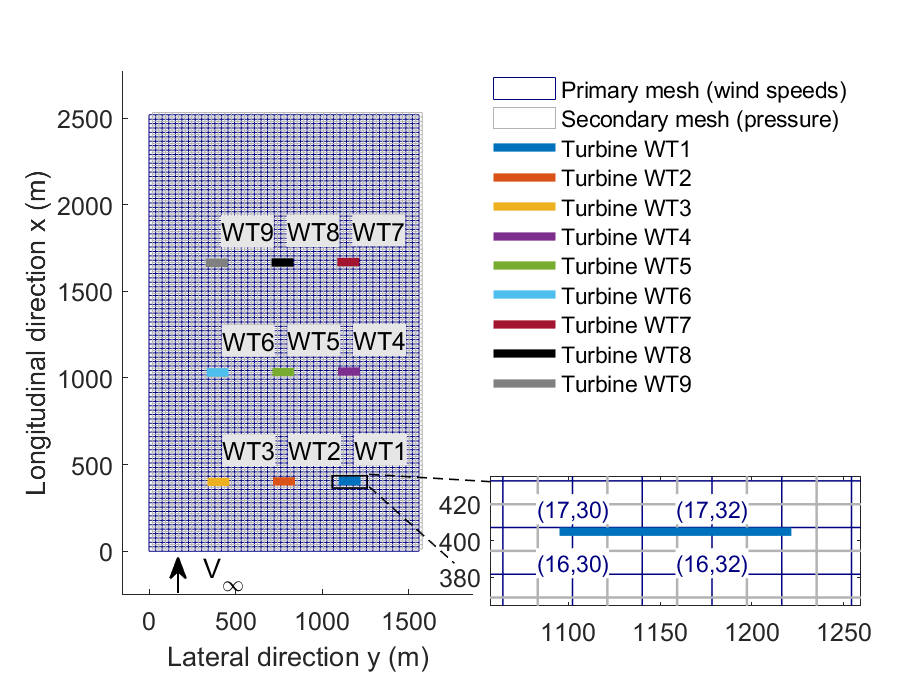
\includegraphics[width=0.7\textwidth,trim={0 0cm 0cm 0.0cm},clip]{figures/figDirETC/gridmesh9_tex.eps}
    \caption[WFSim mesh setup for a nine-turbine wind farm.]{WFSim mesh setup for a nine-turbine wind farm. The primary mesh (blue) is used for wind speed calculations, and the secondary mesh (gray) for pressure. Turbines are shown as colored bars. Zoomed-in area around WT1 shows primary grid point indices.} 
    \label{fig:9TurbMesh}
\end{figure}
The turbine locations for the default nine-turbine wind farm layout included with WFSim are depicted as bold, colored lines. The figure shows the entire wind field area and highlights a zoom around the first turbine, showing that the nodes of the secondary grid correspond to the centers of the primary grid cells and providing the index pair of the node as blue numbers. The effective wind speeds of the turbines are calculated based on the wind speeds at the nodes of the primary grid in front of the turbines. In the example in Figure~\ref{fig:9TurbMesh} the grid points used for the upstream turbine WT1 are the points in the 16th row from the 30th to the 33rd column. For better readability, only every second mesh point is annotated with the corresponding grid index in the zoom on the turbine location.

The finite volume method discretizes Partial Differential Equations (PDEs) such as the NSE by integrating them over small control areas to ensure the conservation of fluxes, such as the air mass flowing through the wind farm, across cell boundaries. In the WFSim 2D simulation, pressure is stored at the center of each grid cell, corresponding to the mesh points of the secondary mesh, while the longitudinal wind speed $v_x$, acting in the vertical direction, is stored at the top and bottom edges and the lateral wind speed $v_y$ is stored at the left and right edges of the primary mesh.

In CFD software, the convective terms from Equation~\eqref{eq:NSE2d} are approximated with a combination of differencing schemes. These schemes compute how the wind carries momentum across the grid by switching between approaches to balance numerical stability and solution accuracy. Upwind differencing, which is more stable, is used where convection dominates diffusion, whereas central differencing, which is more accurate, is used elsewhere. Temporal discretization is performed using an implicit Euler method.
%
Numerical cost varies considerably with grid resolution, timestep, and available computing resources; for example, NREL's SOWFA documentation \cite{churchfield2012overview} reports a coarse LES example that ran at approximately 1.6\,s of wall-clock time per 1\,s of simulated time on 32 cores. Wall-clock time is the total real-world time elapsed from the start to the end of a simulation, including computation, inter-processor communication, disk I/O, memory access, and any idle or waiting time.

In \cite{boersma2018control}, which introduces the WFSim software, a mean computation time of approximately 0.02\,s per 1\,s time step is reported for a two-turbine case with a $50 \times 25$ grid, obtained on a single core notebook with an Intel Core i7-4600U processor instead of a server cluster. In contrast, the computation time of LES can be of the order of days or weeks using distributed computation and generally exceeds the simulated time \cite{boersma2018control}. WFSim was shown to approximate the mean flow centerline velocity and the power of a nine-turbine case simulated with SOWFA reasonably well, with stronger fluctuations of the power signals due to the missing turbine dynamics.
%
In WFSim, the wind field is approximated by a linear system for the velocity and pressure fields at each timestep, resulting in a significant reduction in simulation time and required computing resources. A more detailed overview of WFSim, including equations, is provided in Section~\ref{sec:WindFarmSimulationWFSim}, which also discusses the modifications made to WFSim to obtain the simulation results in \cite{dittmer2022data,dittmer2023koopman}.

\subsection{Wind Farm Control}\label{Subsection:Windfarmcontrol}
In this thesis, WFSim is used as a proof of concept for applying Koopman models to wind farm control, as it natively includes a farm-level MPC for the thrust control signals $C_T^{\prime}$ and supports the yaw angle $\gamma$ as a turbine input. The thrust controls, controlling the energy amount harvested by a turbine, are fictitious inputs used as substitutes for generator torque and blade pitch to avoid the need for a complex turbine model.

For closed-loop wind farm control, turbine control inputs are set to minimize the power reference tracking error and actuator activity, given a wind farm layout, a power grid reference $P_{\text{ref}}$, and the freestream wind speed $V_{\infty}$. Figure \ref{figBlockDiagramFarm} presents a block diagram of the control strategy for a wind farm consisting of two wind turbines.

\begin{figure}[ht]
    \centering
    \includegraphics[width=0.7\textwidth,trim={0 0cm 0cm 0.01cm},clip]{figures/figDirETC/farmCtrl10_PandUr.pdf}
    \caption{Block diagram of closed-loop wind farm control in WFSim}
    \label{figBlockDiagramFarm}
\end{figure}

The wind farm layout and turbine parameters used in this study are consistent with those in \cite{sharan2022Koopman}, \cite{dittmer2022data}, and \cite{dittmer2023koopman}, upon which this thesis is based.

In the MPC implementation included with WFSim, it is assumed that the effective wind speeds at both turbines, $V_{r1}$ and $V_{r2}$, can be measured. These wind speeds, along with the power outputs $P_1$ and $P_2$, and the thrust forces $F_{T,r1}$ and $F_{T,r2}$, serve as feedback for the wind farm controller.

The effective wind speed $V_{ri}$ at the $i$-th turbine is calculated as the mean of the wind speed components normal to the rotor across the $n_r$ rotor grid points:
\begin{align} \label{eqEffWindSpdWT}
    V_{ri}(\gamma_{i}) = \frac{1}{n_r} \sum_{j = 1}^{n_r} \cos(\gamma_{i} + \phi_{ij})\, V_{ij},  
    \quad  V_{ij} = \sqrt{v_{x,ij}^2 + v_{y,ij}^2}, \quad \phi_{ij} = \arctan\left(\frac{v_{y,ij}}{v_{x,ij}}\right),
\end{align}
where $v_{x,ij}$ and $v_{y,ij}$ are the wind speed components in the $x$ and $y$ directions, respectively, at the $j$-th grid point of the $i$-th rotor in the simulated WFSim domain.  The vectors of wind speeds at the grid points directly behind the two turbines are denoted by $\bm{V}_{o1}$ and $\bm{V}_{o2}$. Since the effective wind speed $V_{r2}$ is influenced by the wake of the first turbine, propagating through the wind speeds contained in $\bm{V}_{o1}$, the power and thrust outputs of the second turbine are also affected by the control input of the first turbine. 

The thrust control signal $C_T^{\prime}$ is the thrust coefficient related to the effective wind speed $V_r$ at the rotor instead of the freestream wind speed, i.e., 
\begin{align*}
    C_T^{\prime} = c_T/(1-a)^2 = 4a/(1-a),
\end{align*}
so that the thrust and the power of the ideal actuator disk are
\begin{align*}
    F_{T,r} = \frac{1}{2}\rho_a A_r C_T^{\prime} V_r^2 \quad \text{and} \quad P_r = \frac{1}{2}\rho_a A_r C_T^{\prime} V_r^3.
\end{align*}
The WFSim MPC discrete-time turbine model is given by:
\begin{align} \label{eqPowerWT}
    \begin{split}
        P_{i}(k+1) &= (1 - \tau) P_{i}(k) + \tau \frac{1}{2} \rho_a A_r \left(V_{ri}(\gamma_{i}(k))\right)^3 C_{Ti}^\prime(k), \\
        F_{T,ri}(k+1) &= (1 - \tau) F_{T,ri}(k) + \tau \frac{1}{2} \rho_a A_r \left(V_{ri}(\gamma_{i}(k))\right)^2 C_{Ti}^\prime(k), \\
        \hat{C}_{Ti}^\prime(k+1) &= (1 - \tau) \hat{C}_{Ti}^\prime(k) + \tau C_{Ti}^\prime(k),
    \end{split}
\end{align}
with discrete sample time index $k$ and the constant $\tau$ as a discrete-time filter coefficient that determines the weighting between the current state and the new input at each time step. Larger values of  $\tau$ lead to faster updates. The state vector is defined as $\bm{x}_{\text{WT},i} = [P_i \;\; F_{T,ri} \;\; \hat{C}_{Ti}^\prime]^T$, where $P_i$ is the power and $F_{T,ri}$ is the thrust force of the $i$-th turbine. The third state $\hat{C}_{Ti}^\prime$ is the filtered thrust control signal.

Equation~\eqref{eqPowerWT} is reformulated as
\begin{align} \label{eqWTWFSim}
    \bm{x}_{\text{WT}i}(k+1) =\bm{A}_{\text{WT}i} \bm{x}_{\text{WT}i}(k) +\bm{B}_{\text{WT}i}(V_{ri}(\gamma_i))C_{Ti}^\prime(k), 
\end{align}
with the system and input matrices
\begin{align*}
    \bm{A}_{\text{WTi}} = (1-\tau)\bm{I}_{3\times3},\text{ }\bm{B}_{\text{WTi}} = \tau[ C_P(V_{ri}(\gamma_i(k))) \quad C_F(V_{ri}(\gamma_i)) \quad 1]^T
\end{align*}
where $C_P(V_{ri}(\gamma_i)) = 1/2 \rho_a A_r (V_{ri}(\gamma_{i}))^3$ and $C_F(V_{ri}(\gamma_i)) = 1/2 \rho_a A_r (V_{ri}(\gamma_{i}))^2$.
A concatenation into a wind farm model, with wind vector $\bm{V_r}$ and thrust $\bm{C}_{T}^\prime$ and yaw $\bm{\gamma}$ of all turbines, gives 
\begin{align} \label{eqLinWF}
    \bm{x}_{\text{WF}}(k+1) = \bm{A}_{\text{WF}} \bm{x}_{\text{WF}}(k) + \bm{B}_{\text{WF}}(\bm{V_r}(\bm{\gamma}(k))) \bm{C}_{T}^\prime (k).
\end{align}
It is defined by the block diagonal system and input matrices $\bm{A}_{\text{WF}} \in {\mathbb{R}}^{3n_{\text{WT}} \times 3n_{\text{WT}}}$ and $\bm{B}_{\text{WF}} \in {\mathbb{R}}^{3n_{\text{WT}} \times n_{\text{WT}}}$ with turbine system and input matrices on their diagonals, and farm state $\bm{x}_{\text{WF}} \in {\mathbb{R}}^{3n_{\text{WT}}}$ for a farm with $n_{\text{WT}}$ turbines.

The models presented in Equations~\eqref{eqWTWFSim} and \eqref{eqLinWF} form the foundation of the wind farm baseline MPC algorithm and the adaptive AIC qLMPC presented in this thesis. The theoretical frameworks required to design and implement MPC algorithms are introduced in Section~\ref{sec:Control-Theoretic Background}.

\section{Control-Theoretic Background}\label{sec:Control-Theoretic Background}
The following sections introduce the two modeling frameworks applied in this thesis, where first-principles-based qLPV models are used for wind turbines and Koopman-theory-based data-driven models for wind farms. This is followed by the MPC framework applied to both turbines and farms.

\subsection{Quasi-Linear Parameter-Varying Models}
\label{sec:qLPVmodels}
As described in the previous section, wind turbine dynamics are characterized by nonlinearities due to aerodynamic and structural effects. To leverage extensive existing linear control and estimation frameworks, Linear Parameter-Varying (LPV) models and their generalized form, quasi-LPV (qLPV) models, can be used to represent nonlinear dynamics through a linear structure with time-varying parameters \cite{hoffmann2014survey}. These scheduling parameters capture the nonlinearity while preserving computational efficiency and physical interpretability. In the context of WECS, qLPV modeling enables systematic controller design across the entire operating range of a turbine without requiring full nonlinear computations at each time step.

\subsubsection{Standard and Velocity-based qLPV Models}
\label{sec:qLPVmodelTheory}

In general, nonlinear continuous-time dynamics can be expressed as
\begin{align} \label{eq:stateSpaceGeneral}
    \dot{\bm{x}}(t) = \bm{f}(\bm{x}, \bm{u}), \quad
    \bm{y}(t) = \bm{h}(\bm{x}, \bm{u}),
\end{align}
with the state $\bm{x} \in \mathbb{R}^{n_x}$, input $\bm{u} \in \mathbb{R}^{n_u }$, and output $\bm{y} \in \mathbb{R}^{n_y }$. The functions $\bm{f}$ and $\bm{h}$ are nonlinear, but locally smooth in the neighborhood of operating points.

The matrices of the LPV model are obtained by linearizing Equation~\eqref{eq:stateSpaceGeneral} around relevant operating points, yielding the Jacobian-based matrices
\begin{equation}\label{eq:contMatricesqLPV}
    \begin{aligned}
        \bm{A}_c(\bm{x},\bm{u}) &= \nabla_{\bm{x}} \bm{f}(\bm{x},\bm{u}) \in \mathbb{R}^{n_x \times n_x}, \quad
        \bm{B}_c(\bm{x},\bm{u}) = \nabla_{\bm{u}} \bm{f}(\bm{x},\bm{u}) \in \mathbb{R}^{n_x \times n_u}, \\
        \bm{C}_c(\bm{x},\bm{u}) &= \nabla_{\bm{x}} \bm{h}(\bm{x},\bm{u}) \in \mathbb{R}^{n_y \times n_x}, \quad
        \bm{D}_c(\bm{x},\bm{u}) = \nabla_{\bm{u}} \bm{h}(\bm{x},\bm{u})\in \mathbb{R}^{n_y \times n_u}.
    \end{aligned}
\end{equation}
The scheduling parameter vector $\bm{\rho}_\Rho$ is constructed from selected states and inputs, and the qLPV model becomes:

\begin{equation} \label{eq:standardqLPV1}
    \begin{aligned}
        \dot{\bm{x}}(t) &= \bm{A}_c(\bm{\rho}_\Rho) \bm{x}(t) + \bm{B}_c(\bm{\rho}_\Rho) \bm{u}(t), \\
        \bm{y}(t) &= \bm{C}_c(\bm{\rho}_\Rho) \bm{x}(t) + \bm{D}_c(\bm{\rho}_\Rho) \bm{u}(t). 
    \end{aligned}
\end{equation}
Here, $\bm{x}$, $\bm{u}$, and $\bm{y}$ denote deviations from the respective operating point. If the scheduling parameter $\bm{\rho}_\Rho$ depends solely on exogenous variables (i.e., external signals such as the freestream wind speed), the system is strictly LPV. However, if $\bm{\rho}_\Rho$ depends additionally or purely on endogenous variables (i.e., system states), as in the wind turbine and farm models discussed here, the resulting structure is a qLPV model. This distinction is important as the dependence on model states introduces implicit dependencies that must be accounted for during control design. In the case of qLPV models used for MPC, the scheduling parameter has to be specified for all samples of the prediction horizon to calculate the prediction trajectory as a function of the states, e.g., from the trajectory predicted at the previous sample, see~\cite{cisneros2016efficient}.

An alternative, velocity-based qLPV formulation considers the derivatives of state and input rather than the states and inputs themselves \cite{cisneros2020velocity}. Differentiating Equation~\eqref{eq:stateSpaceGeneral} with respect to time gives:
\begin{align*}
    \ddot{\bm{x}}(t) &= \bm{A}_c(\bm{\rho}_\Rho) \dot{\bm{x}}(t) +\bm{B}_c(\bm{\rho}_\Rho) \dot{\bm{u}}(t), \\
    \dot{\bm{y}}(t) &= \bm{C}_c(\bm{\rho}_\Rho)  \dot{\bm{x}}(t) + \bm{D}_c(\bm{\rho}_\Rho) \dot{\bm{u}}(t).
\end{align*}
This velocity-based form has the advantage of steady-state behavior at the origin ($\dot{\bm{x}}=\dot{\bm{u}}=0$), eliminating the need to store equilibrium state and input vectors at each operating point. Therefore, no trimming calculations are required once a physical model is derived based on the nonlinear dynamics. 

The wind turbine qLMPC presented in this thesis is formulated in discrete time within a velocity-based qLPV framework. The matrices $\bm{A}_d\in \mathbb{R}^{n_x \times n_x}$ and $\bm{B}_d\in \mathbb{R}^{n_x \times n_u}$ of the discrete velocity form can be obtained via zero-order hold discretization from their continuous-time counterparts from Equation~\eqref{eq:contMatricesqLPV}:
\begin{equation} \label{eq:zoh1}
    \begin{aligned}
        \bm{A}_d(\bm{\rho}_\Rho) &= e^{\bm{A}_c(\bm{\rho}_\Rho)T_s}, \\
        \bm{B}_d(\bm{\rho}_\Rho) &= \left( \int_0^{T_s} e^{\bm{A}_c(\bm{\rho}_\Rho)\tau} \, d\tau \right) \bm{B}_c(\bm{\rho}_\Rho),
    \end{aligned}
\end{equation}
with the sample time $T_s$. A velocity-based discrete state-space model can then be set up as:
\begin{align} \label{eq:velocityFormDisc}
    \Delta\bm{x}(k+1) = \bm{A}_d(\bm{\rho}_\Rho) \Delta\bm{x}(k) + \bm{B}_d(\bm{\rho}_\Rho) \Delta\bm{u}(k),
\end{align}
with $\Delta\bm{x}(k) = \bm{x}(k) - \bm{x}(k-1)$ and $\Delta\bm{u}(k) = \bm{u}(k) - \bm{u}(k-1).$

A subset of states $\bm{x}_{\text{sel}} \in \mathbb{R}^{n_{\text{sel}}}$ is selected for explicit inclusion in the qLPV model's state vector, enabling direct constraints on these states within the MPC scheme. The discrete difference vector $\Delta\bm{x}(k)$ at time sample $k$ is augmented with the vector 
\begin{equation}  \label{eq:differenceSelectedFormDisc}
    \begin{aligned}
        \bm{x}_{\text{sel}}(k) &= \bm{x}_{\text{sel}}(k-1) + \Delta \bm{x}_{\text{sel}}(k) \\ 
        &=  \bm{x}_{\text{sel}}(k-1) +  \bm{A}_{d,\text{sel}}\Delta \bm{x}(k-1) +  \bm{B}_{d,\text{sel}}\Delta \bm{u}(k-1),   
    \end{aligned}
\end{equation}
with the matrices $\bm{A}_{d,\text{sel}} \in  \mathbb{R}^{n_{\text{sel}} \times n_x}$ and  $\bm{B}_{d,\text{sel}} \in  \mathbb{R}^{n_{\text{sel}} \times n_u}$ representing the rows of the state and input matrices corresponding to the selected states.

The resulting augmented state-space model with the expanded state vector $\bm{x}_{\text{ext}} =[\bm{x}_{\text{sel}}^T \; \; \Delta\bm{x}^T ]^T$ is derived based on the matrices used in Equations~\eqref{eq:velocityFormDisc} and~\eqref{eq:differenceSelectedFormDisc}:
\begin{equation}\label{eq:discreteVelocityqLPV}
    \begin{aligned}
        \begin{bmatrix} \bm{x}_{\text{sel}}(k+1) \\ \Delta\bm{x}(k+1) \end{bmatrix} 
        &= \begin{bmatrix} \bm{I}_{n_{\text{sel}}} & \bm{A}_{d,\text{sel}}(\bm{\rho}_\Rho) \\ 
            \bm{0}_{n_x \times n_\text{sel}} & \bm{A}_d(\bm{\rho}_\Rho) 
        \end{bmatrix}
        \begin{bmatrix} \bm{x}_{\text{sel}}(k) \\ \Delta\bm{x}(k) \end{bmatrix}
        + \begin{bmatrix} \bm{B}_{d,\text{sel}}(\bm{\rho}_\Rho) \\ \bm{B}_d(\bm{\rho}_\Rho) \end{bmatrix} \Delta\bm{u}(k), \\
        \bm{y}(k) &= \bm{x}_{\text{sel}}(k) = \begin{bmatrix} \bm{I}_{n_{\text{sel}}} & \bm{0}_{n_\text{sel} \times n_x} \end{bmatrix} 
        \begin{bmatrix} \bm{x}_{\text{sel}}(k) \\ \Delta\bm{x}(k) \end{bmatrix},
    \end{aligned}
\end{equation}
where both the selected states and the discrete differences of all states appear explicitly in the dynamics. 

This structured state expansion, necessary for velocity-based qLPV models used in constrained MPC algorithms, increases, and may even double, the state dimension. This complicates stability analysis and controller synthesis using robustness guarantees such as Linear Matrix Inequality (LMI) schemes. However, for the low-order MPC implementation presented here, the increased state dimension is not critical, and LMI-based robustness guarantees are not pursued.

Finally, the qLPV framework approximates nonlinear dynamic systems by allowing the model matrices to vary smoothly over the operating range. This can be achieved in several ways, for example through precomputed local linearizations, data-driven identification, or first-principles models combined with physics-based lookup tables. In this work, a combination of first-principles models and physics-based lookup tables is used.


\subsubsection{qLPV Models based on BEM Models and Actuator Disk Models}
\label{sec:quasi-LPVTurbineModel}

For wind energy applications, the mapping from the disturbance input wind speed and the control inputs generator torque and pitch angle to turbine states, including, e.g., rotor speed and tower displacement, is obtained from the mathematical representations of wind turbine physics described in Section~\ref{windTurbineModel}. For the turbine models in this work, two-dimensional lookup tables for the thrust and torque coefficients are derived from BEM models implemented in the FAST software. They depend on the collective blade pitch angle $\beta_0$ and the tip-speed ratio
\begin{equation} \label{eq:lambda}
    \lambda = \frac{\omega_r R_r}{V_\infty},
\end{equation}
i.e., the ratio of the blade tip speed, given by the rotor speed $\omega_r$ and the rotor radius $R_r$, to the freestream wind speed $V_\infty$. Thus, they depend on wind speed, rotor speed, and pitch angle. When these nonlinear aerodynamic relationships are combined with the linear tower and drivetrain dynamics, the overall model becomes a nonlinear Ordinary Differential Equation (ODE) system that can be approximated locally as linear around each operating point. For the BEM-based turbine model, the scheduling vector
\begin{equation} \label{eq:rhoWT}
    \bm{\rho}_{\Rho,\text{WT}} = [V_\infty \quad \beta_0 \quad \omega_r]^T,
\end{equation}
consisting of wind speed, pitch angle, and rotor speed, captures the variations in the aerodynamics. The qLPV matrices thus reflect that changes in these three parameters immediately influence the aerodynamic behavior of the turbine. Note that in the models used for controller design, the pitch angle $\beta_0$ is a state, while the commanded pitch $\beta_{0,\text{ref}}$ is the input, see Equation~\eqref{eq:11} in Chapter~\ref{sec:WindTurbineqLPVModels}. Chapter~\ref{sec:WindTurbineqLPVModels} provides a detailed derivation of two qLPV wind turbine models, both based on lookup tables for the thrust and torque coefficients generated using FAST.

For farm-level control, the turbines are represented by the actuator disk model from Section~\ref{windTurbineModel}. Its input matrices depend on the effective inflow wind speeds of the $n_{\text{WT}}$ turbines, which therefore serve as the scheduling parameters of the qLPV wind farm model:
\begin{equation} \label{eq:rhoWF}
    \bm{\rho}_{\Rho,\text{WF}} = [V_{r1} \quad V_{r2} \quad \ldots \quad V_{r n_{\text{WT}}}]^T.
\end{equation}
These effective wind speeds depend on exogenous variables, i.e., the freestream wind including its turbulence, and on endogenous system states, i.e., the filtered thrust coefficients $\hat{C}^\prime_{Ti}$ of the upstream turbines. These signals follow the commanded thrust control inputs $C^\prime_{Ti}$. The scheduling parameters are hence partially state-dependent, which is the defining feature of a qLPV model. Chapter~\ref{sec:ApplicationtoWindFarmControl} describes how these effective wind speeds are predicted with a Koopman model and used in the qLPV wind farm controller.

By combining these qLPV representations with predictive control formulations, one can design MPC controllers that explicitly accommodate nonlinear aerodynamic effects while maintaining convex optimization structure. 


%The qLPV wind farm model used in the MPC formulation implemented in WFSim (see Section~2.3.2) is a representative example.

\subsection{Koopman Theory for System Modeling} \label{sec:Koopman}

This section presents the principle of Koopman operators, followed by a description of the design of the Koopman matrix as a prediction scheme based on Koopman operators. The Koopman framework allows the representation of any finite-dimensional nonlinear system as an infinite-dimensional linear system. Two variants of Dynamic Mode Decomposition (DMD), Extended DMD (EDMD) and Extended Input-Output DMD (EIODMD), are used in this work for finite matrix approximations of the infinite-dimensional Koopman operator. This thesis leverages notations and methods from \cite{arbabi2018data}, where a data-driven Koopman MPC framework for nonlinear PDEs was presented. The approach identifies a Koopman-linear model via EDMD to design a feedback controller, demonstrated on Burgers’ equation and NSE cavity flow. The latter example is particularly relevant to wind farm control, as both are governed by NSE.

\subsubsection{Koopman Operator and Matrix}\label{KoopmanOperator}

The Koopman operator $\mathcal{K}$ provides a framework for transforming finite-dimensional nonlinear dynamics into an infinite-dimensional linear system. By approximating this operator with a finite-dimensional representation, the tools of linear system analysis and control theory can be directly applied to nonlinear systems. This approach was originally proposed in \cite{koopman1931hamiltonian}. For its application to control, see, e.g., \cite{proctor2018generalizing} or \cite{kaiser2020data}.

Consider a time-invariant, discrete-time autonomous nonlinear dynamical
system with state $\bm{x}(k) \in \mathbb{R}^{n_x}$ and state-transition
map $F: \mathbb{R}^{n_x} \to \mathbb{R}^{n_x}$:
\begin{equation}
    \bm{x}(k+1) = F(\bm{x}(k)).
    \label{eq:nonLinSysKoop}
\end{equation}
%
The Koopman framework describes nonlinear dynamics through the evolution
of functions of the state, rather than the state $\bm{x}$ itself. It
thus represents the dynamics as a linear system in a suitable function
space. These functions are referred to as lifting functions. A collection of
lifting functions evaluated at the current state defines the lifted state.

Let $g_\infty$ denote an infinite-dimensional lifting map whose component
functions belong to a suitable Hilbert space $\mathcal{H}$
\footnote{A Hilbert space is a complete inner-product space that
    generalizes Euclidean space to potentially infinite dimensions
    \cite{korda2018linear}.}.
The corresponding lifted state is infinite-dimensional:
\begin{equation}
    \bm{\varphi}_\infty(k) = g_\infty(\bm{x}(k)).
\end{equation}
%
The linear, infinite-dimensional Koopman operator
$\mathcal{K}: \mathcal{H} \to \mathcal{H}$ acts on the lifting function
$g \in \mathcal{H}$ according to
\begin{equation}
    (\mathcal{K}g)(\bm{x}) = g(F(\bm{x})).
\end{equation}
%
Applying the Koopman operator componentwise to $g_\infty$ yields the
evolution of the lifted state:
\begin{equation}
    \begin{aligned}
        \bm{\varphi}_\infty(k+1)
        &= (\mathcal{K}g_\infty)(\bm{x}(k)) \\
        &= g_\infty(F(\bm{x}(k))) \\
        &= g_\infty(\bm{x}(k+1)).
    \end{aligned}
    \label{eq:KoopmanUnforced}
\end{equation}
%
Figure~\ref{fig:koopman-diagram} visualizes the concept of a Koopman operator applied to an unforced nonlinear system, as described in Equations~\eqref{eq:nonLinSysKoop} to \eqref{eq:KoopmanUnforced}.
\begin{figure}[htb]
    \centering
    \includegraphics[width=0.82\textwidth, trim=0cm 0cm 0cm 0cm, clip]{figures/figuresBlockDiagram_IFAC23/KoopmanDiagram.pdf}
    \caption{Block diagram of the nonlinear system, lifting function, and linear Koopman operator propagation for an unforced system (adapted from \cite{brunton2016koopman}).} 
    \label{fig:koopman-diagram}
\end{figure}
The solid arrows show the main process flow. The dashed arcs indicate that the original states can be reconstructed from the lifted states and dash-dotted arrows represent the states' links to previous and future states.

Because the Koopman operator $\mathcal{K}$ is infinite-dimensional, it generally cannot be used directly for real-time control calculations. This work hence employs a finite-dimensional approximation. A truncated lifting function $g: \mathbb{R}^{n_{x}} \to \mathbb{R}^{n_{g}}$ is used to create the approximated lifted state $\bm{\varphi} \in \mathbb{R}^{n_{g}}$:
\begin{equation}
    \bm{\varphi}(k) = g(\bm{x}(k)). \label{eq:observ}
\end{equation}
By defining $g$ as a finite subset of $\mathcal{H}$, the operator $\mathcal{K}$ can be approximated by a finite-dimensional Koopman matrix $\hat{K}$. Note that in the following the truncated lifting functions and approximated lifted states are simply referred to as lifting function and lifted states, respectively, for better readability.
%
This definition extends to nonlinear systems with input $\bm{w}$ as follows. The Koopman operator for controlled systems evolves on the extended state space $\mathbb{R}^{n_{x}} \times \ell(\mathcal{W})$, where $\ell(\mathcal{W})$ denotes the space of all infinite discrete input sequences $\bm{w} = (\bm{w}(k))_{k=1}^\infty$ \cite{arbabi2018data, korda2018linear}. The extended state vector 
\[
\bm{x}_w(k) = \begin{bmatrix} \bm{x}(k) \\ \bm{w}(k) \end{bmatrix} \in \mathbb{R}^{n_x + n_w}
\]
evolves according to the extended dynamics
\begin{align} \label{eq:KoopStateForced}
    \bm{x}_w(k+1) = \tilde{F}_w(\bm{x}(k), \bm{w}(k)) = \begin{bmatrix} F_w(\bm{x}(k), \bm{w}(k)) \\ S(\bm{w}(k)) \end{bmatrix} = \begin{bmatrix} \bm{x}(k+1) \\ \bm{w}(k+1) \end{bmatrix},
\end{align}
where $F_w$ defines the state transition and the input sequence is moved forward by the shift operator $S$, defined by $S\left( (\bm{w}(k))_{k=1}^\infty \right) = (\bm{w}(k+1))_{k=1}^\infty$. The augmented flow map $\tilde{F}_w$ captures both the state transitions and the evolution of the exogenous signal.

The Koopman operator acts on the lifted states $\bm{\varphi}_w$ within the function space of the lifting function $g$. In practice, this infinite-dimensional operator is approximated by a finite-dimensional Koopman matrix 
\begin{align*}
    \hat{\bm{K}} = [\bm{A}_K \;\; \bm{B}_K].
\end{align*}
This matrix maps the current extended lifted state to the next prediction:
\[
\bm{\varphi}(k+1) \approx \hat{\bm{K}} \bm{\varphi}_w(k) = [\bm{A}_K \;\; \bm{B}_K] \begin{bmatrix} \bm{\varphi}(k) \\ \bm{w}(k) \end{bmatrix},
\]
consistent with \cite{arbabi2018data, korda2018linear} and illustrated in Figure~\ref{fig:koopman-diagram-ext}. 
\begin{figure}[htbp]
    \centering
    \includegraphics[width=0.95\textwidth, trim=0.cm 0.cm 0.cm 0cm, clip]{figures/figuresBlockDiagram_IFAC23/KoopmanDiagramExt.pdf}
    \caption{Block diagram of the nonlinear system, approximated lifting function, shift operator, and Koopman matrix propagation for a forced system (adapted from \cite{proctor2018generalizing}).}
    \label{fig:koopman-diagram-ext}
\end{figure}

This includes the extended state dynamics \(F_w\), the shift operator \(S\) acting on the input sequence, lifting functions \(g_w\) that map states and inputs to the extended, lifted observable space $\bm{\varphi}$, the Koopman matrix \(\hat{K}\) propagating lifted states and the lifted state at the next sample  $\bm{\varphi}(k+1)$ derived from the extended, lifted state $\bm{\varphi}_w(k)$. As before, dashed arrows indicate that the original states and inputs can be recovered from the lifted states.
%
An illustrative example of lifting nonlinear dynamics into a higher-dimensional linear system is given in \cite{brunton2016koopman}. Consider the discrete-time nonlinear system
\begin{align} \label{eq:BruntonEx1}
    x_1(k+1) &= \mu x_1(k), \\
    x_2(k+1) &= \lambda x_2(k) - \lambda x_1^2(k) + u(k),
\end{align}
where \( x_1, x_2 \in \mathbb{R} \), \( \mu, \lambda \in \mathbb{R} \), and \( u \in \mathbb{R} \) is a scalar control input. The system is clearly nonlinear due to the \( x_1^2(k) \) term. By introducing a new observable \( \varphi(k) = x_1^2(k) \), the system can be rewritten as 
\begin{equation} \label{eq:BruntonEx2}
    \varphi(k+1) = x_1^2(k+1) = \mu^2 x_1^2(k) = \mu^2 \varphi(k),
\end{equation}
which evolves linearly. Leveraging Equations~\eqref{eq:BruntonEx1} to~\eqref{eq:BruntonEx2} to stack the states and the observable into a lifted state vector, the dynamics can be expressed as a linear system:
\begin{equation}
    \begin{bmatrix}
        x_1(k+1) \\
        x_2(k+1) \\
        \varphi(k+1)
    \end{bmatrix}
    =
    \begin{bmatrix}
        \mu & 0 & 0 \\
        0 & \lambda & -\lambda \\
        0 & 0 & \mu^2
    \end{bmatrix}
    \begin{bmatrix}
        x_1(k) \\
        x_2(k) \\
        \varphi(k)
    \end{bmatrix}
    +
    \begin{bmatrix}
        0 \\
        1 \\
        0
    \end{bmatrix}
    u(k).
\end{equation}
This construction yields a finite-dimensional linear representation of the original nonlinear system in lifted coordinates, where the Koopman operator corresponds to a matrix multiplication.

However, the Koopman operator cannot always be represented as a matrix multiplication. As shown in \cite{brunton2016koopman}, systems with multiple fixed points, periodic orbits, or attracting/repelling structures cannot be exactly represented by a finite-dimensional Koopman model, as finite-dimensional linear systems cannot have multiple isolated equilibrium points.
%In \cite{brunton2016koopman}, it is stated:
%\begin{quote}
%For any system with multiple fixed points, periodic orbits, or attracting/repelling structures, 
%there is no finite-dimensional Koopman invariant subspace that explicitly includes the state. 
%This follows from the fact that these systems cannot be topologically conjugate 
%to a finite-dimensional linear system with a single fixed point.
%\end{quote}
%In other words, any finite-dimensional linear system can only have one equilibrium point, 
%so it cannot exactly capture the behavior of more complex nonlinear systems.
As a discrete-time example where the Koopman operator is infinite-dimensional,  the scalar nonlinear system
\begin{equation}
    x(k+1) = \mu x^2(k), \quad x \in \mathbb{R}, \ \mu \in \mathbb{R}
\end{equation}
is considered. Note that this system has two fixed points, which are $x=0$ and $x=1/\mu$ for $\mu \neq 0$. The fixed point at the origin is attracting, since $f'(0)=0$, 
while the fixed point at $x=1/\mu$ is repelling, since $f'(1/\mu)=2$ with $|2|>1$. Defining the observable \( \varphi_1 = x^2 \) leads to
\begin{equation}
    \varphi_1(k+1) = x^2(k+1) = (\mu x^2(k))^2 = \mu^2 x^4(k),
\end{equation}
which introduces the need for a new observable \( \varphi_2 = x^4 \). Continuing this process,
\begin{equation}
    \varphi_2(k+1) = x^4(k+1) = (\mu x^2(k))^4 = \mu^4 x^8(k),
\end{equation}
and so on, yields an infinite sequence of new lifted states, i.e., no finite set of polynomial lifted states represents the system. More generally, as the system has two isolated fixed points, there is no finite-dimensional Koopman-invariant subspace that contains the state $x$ itself \cite{brunton2016koopman}.

In cases where the Koopman operator is infinite-dimensional, one approach is to approximate it with a finite matrix using a suitable set of lifted states. This Koopman matrix can be identified directly from data by DMD, without requiring a closed-form model of the underlying dynamics. This makes the approach applicable to wind farm control, where the flow and wake dynamics are governed by the NSE, for which no general analytical solution is known and whose discretization yields a state dimension far too large for an analytical lifting.


\subsubsection{Koopman Matrix for Wind Farm Modeling}\label{KoopmanIdentification}

In this work, the effective wind speeds acting on the turbines are included in the states of the Koopman models. For the qLMPC design, which predicts the effective wind speeds from the thrust control signals, EDMD is used. For the linear Koopman MPC design, which predicts the farm power directly, EIODMD is applied.

The discrete-time nonlinear dynamical system can be extended by an output $\bm{y}$ as
\begin{equation}
    \bm{x}(k+1) = F_w(\bm{x}(k), \bm{w}(k)), \quad 
    \bm{y}(k) = G(\bm{x}(k), \bm{w}(k)) \label{eq:nonLinSys}
\end{equation}
with states $\bm{x} \in \mathbb{R}^{n_{x}}$, inputs $\bm{w} \in \mathbb{R}^{n_{w}}$, outputs $\bm{y} \in \mathbb{R}^{n_{y}}$, and nonlinear functions $F_w : \mathbb{R}^{n_{x}} \times \mathbb{R}^{n_{w}} \to \mathbb{R}^{n_{x}}$ and $G : \mathbb{R}^{n_{x}} \times \mathbb{R}^{n_{w}} \to \mathbb{R}^{n_{y}}$.


Lifting functions $g$ are defined as before as nonlinear combinations of the original states $\bm{x}$. In this work, a new state $\bm{\varphi}\in\mathbb{R}^{n_{g}}$ is defined as a concatenation of the state $\bm{x}$ and the nonlinear combination of the states $g_{\varphi}$, i.e., the lifted states $\bm{\varphi}_g = g_{\varphi}(\bm{x})$, and hence $ \bm{\varphi} = g(\bm{x})$ with $\bm{\varphi} = [\bm{x}^T \; \bm{\varphi}_g^T]^T$.
%
A finite linear approximation of the nonlinear system given in Equation~\eqref{eq:nonLinSys} is:
\begin{align*}
    \bm{\varphi}(k+1)=\bm{A}_{\hat{K}}\bm{\varphi}(k)+\bm{B}_{\hat{K}}\bm{w}(k), \quad 
    \hat{\bm{y}}(k) = \bm{C}_{\hat{K}}\bm{\varphi}(k) + \bm{D}_{\hat{K}}\bm{w}(k),%\label{eq:linearPredictor}
\end{align*}
where $\hat{\bm{y}}$ is the predicted output vector, $\bm{A}_{\hat{K}}\in \mathbb{R}^{{n_g}\times {n_g}}$, $\bm{B}_{\hat{K}}\in \mathbb{R}^{n_g\times n_w}$, $\bm{C}_{\hat{K}}\in \mathbb{R}^{n_y\times n_g}$, and $\bm{D}_{\hat{K}}\in \mathbb{R}^{n_y\times n_w}$.

For EIODMD, data from $n_o$ samples containing the measured state, input, and output vectors are collected and organized into two data matrices. The first matrix, $\bm{X}_{\text{EIODMD}}$, contains the state and input snapshots. The second matrix, $\bm{X}_{\text{EIODMD},+}$, contains the subsequent state snapshots and the corresponding outputs:
\begin{align} \label{eq:DataCollAIC5}
    \bm{X}_{\text{EIODMD}} &= \begin{bmatrix} 
        \bm{x}(1) & \bm{x}(2) & \dots & \bm{x}(n_o-1) \\
        \bm{w}(1) & \bm{w}(2) & \dots & \bm{w}(n_o-1)
    \end{bmatrix} \in \mathbb{R}^{(n_x+n_w)\times (n_o-1)}, \\
    \bm{X}_{\text{EIODMD},+} &= \begin{bmatrix} 
        \bm{x}(2) & \bm{x}(3) & \dots & \bm{x}(n_o) \\
        \bm{y}(1) & \bm{y}(2) & \dots & \bm{y}(n_o-1)
    \end{bmatrix} \in \mathbb{R}^{(n_x+n_y)\times (n_o-1)}.
\end{align}
%
The matrices $\bm{A}_{\hat{K}}, \bm{B}_{\hat{K}}, \bm{C}_{\hat{K}}$, and $\bm{D}_{\hat{K}}$ can be obtained by solving the optimization problem:
\begin{equation}
    \min_{\hat{K}} \sum_{k=1}^{n_{o}-1} \left\Vert \begin{bmatrix}
        \bm{\varphi}(k+1)\\ \bm{y}(k)
    \end{bmatrix} - \hat{K} \begin{bmatrix}
        \bm{\varphi}(k)\\ \bm{w}(k)
    \end{bmatrix} \right\Vert_{2}^{2} \label{eq:ApproxKalman}
\end{equation}
with the Koopman matrix defined as:
\begin{align*}
    \hat{K} = \begin{bmatrix}
        \bm{A}_{\hat{K}} & \bm{B}_{\hat{K}}\\ 
        \bm{C}_{\hat{K}} & \bm{D}_{\hat{K}} 
    \end{bmatrix} \in \mathbb{R}^{(n_g + n_y) \times (n_g + n_w)}.
\end{align*}
%
The lifting functions are applied to data from the matrices $\bm{X}_{\text{EIODMD}}$ and $\bm{X}_{\text{EIODMD},+}$ to construct two matrices containing these lifted states:
\begin{align}
    \bm{G}_w &= \begin{bmatrix} 
        \bm{\varphi}(1) & \cdots & \bm{\varphi}(n_{o}-1)\\
        \bm{w}(1) & \cdots & \bm{w}(n_{o}-1) 
    \end{bmatrix} \in \mathbb{R}^{(n_g + n_w) \times (n_o - 1)}, \\
    \bm{G}_{+} &= \begin{bmatrix}
        \bm{\varphi}(2) & \cdots & \bm{\varphi}(n_{o})\\
        \bm{y}(1) & \cdots & \bm{y}(n_{o}-1)
    \end{bmatrix} \in \mathbb{R}^{(n_g + n_y) \times (n_o - 1)}. \label{eq:Lplus}
\end{align}
%
The optimization problem \eqref{eq:ApproxKalman} is reformulated as:
\[
\min_{\hat{K}} \left\Vert \bm{G}_{+} - \hat{K} \bm{G}_w \right\Vert_{F}^{2},
\]
where \( \left\Vert \cdot \right\Vert_{F} \) denotes the Frobenius norm. The analytical solution to this linear least squares problem is:
\begin{align*}
    \hat{K} = \bm{G}_{+} \bm{G}_w^{\dagger},
\end{align*}
where \( ^{\dagger} \) denotes the Moore–Penrose pseudoinverse. For EDMD, only the upper part of the Koopman matrix \( \hat{K} \), denoted as \( \hat{K}_u \), which contains the system and input matrices, is used:
\begin{align}
    \hat{K}_u = \begin{bmatrix} \bm{A}_{\hat{K}} & \bm{B}_{\hat{K}} \end{bmatrix}.
\end{align}
This matrix can be derived from the following problem:
\begin{equation}
    \min_{\hat{K}_u} \sum_{k=1}^{n_{o}-1} \left\Vert
    \bm{\varphi}(k+1) - \hat{K}_u
    \begin{bmatrix}
        \bm{\varphi}(k)\\ \bm{w}_u(k)
    \end{bmatrix}
    \right\Vert_{2}^{2}
    \label{eq:ApproxKalmanEDMD}
\end{equation}
with the corresponding solution:
\begin{align*}
    \hat{K}_u = \bm{G}_{+,u} \bm{G}_{w,u}^{\dagger},
\end{align*}
where \( \bm{G}_{+,u} \) is the upper part of the matrix \( \bm{G}_{+} \), as defined in Equation~\eqref{eq:Lplus}, i.e., the concatenation of samples of the vector \( \bm{\varphi} \) at different time steps. The input is denoted \( \bm{w}_u \), as it differs from the input used for EIODMD. The matrix $\bm G_{w,u}$ is built from $\bm\varphi$ and $\bm w_u$.
%
Figure~\ref{fig:BlockEDMDEIODMD} shows the inputs and outputs of the EDMD and EIODMD models.
\begin{figure}[h]
    \centering
    \subfloat[EDMD]{%
        \includegraphics[width=0.35\textwidth, trim=0 0 0 0.5cm, clip]
        {figures/figuresBlockDiagram_IFAC23/farm1_OL2.pdf}}%
    \hspace{0.05\textwidth}
    \subfloat[EIODMD]{%
        \includegraphics[width=0.35\textwidth, trim=0 0 0 0.55cm, clip]
        {figures/figuresBlockDiagram_IFAC23/EIODMD.pdf}}
    \caption{Inputs and outputs of the EDMD and EIODMD models with lifted states $\bm{\varphi}$ based on effective wind speeds $V_{r1}$ and $V_{r2}$.}
    \label{fig:BlockEDMDEIODMD}
\end{figure}
%
The states used to construct both models are the effective wind speeds acting on the turbines, specifically \( V_{r1} \) and \( V_{r2} \), along with lifted states derived from them. The squares and cubes of the effective wind speeds are utilized as they correspond to aerodynamic force and power dependencies.  The lifted state vector of the AIC scheme's EDMD model is therefore:
\begin{align*}
    \bm{\varphi} = [V_{r1} \quad V_{r2} \quad V^2_{r1} \quad V^2_{r2} \quad  V^3_{r1} \quad V^3_{r2}]^T \in \mathbb{R}^6.
\end{align*}
For the combined WRC and AIC (WRC-AIC), the lifted state of the EIODMD model is extended by the filtered control signals, nonlinear features of the control signals, moving means, and a bias state to 21 states, see Section~\ref{sec:lifting functions for Combined Yaw and Thrust Control}.
%
For EDMD, the inputs are the thrust control inputs. For EIODMD, the inputs are the thrust control inputs as well as the yaw control input of the first turbine, since EIODMD is applied in a combined thrust and yaw control setting. Hence, the inputs are:
\begin{align*}
    \bm{w}_{u} = [C^{\prime}_{T1} \quad C^{\prime}_{T2}]^T \in \mathbb{R}^2 \quad\text{and} \quad
    \bm{w} = [C^{\prime}_{T1} \quad C^{\prime}_{T2} \quad \gamma_1]^T \in \mathbb{R}^3.
\end{align*}
The output of the EDMD model consists of the two states \( V_{r1} \) and \( V_{r2} \), whereas the output of the EIODMD model is the total wind farm power, i.e., the sum of the power outputs of both turbines.

While data-driven approaches such as EIODMD for Koopman MPC are particularly 
suitable for wind farm control, where complex wake interactions make first-principles 
modeling challenging, they may not be the optimal choice for individual wind turbines. 
The dynamics of a single turbine are well understood and can be accurately described 
using ODEs, making first-principles-based control strategies more appropriate, with qLMPC being investigated in this work. 

%The following section explores the use of the qLPV framework, which leverages known turbine physics for efficient and reliable control design.

\subsection{Model Predictive Control}
Model Predictive Control (MPC) is an optimization-based control strategy that computes control inputs by repeatedly solving a finite-horizon optimal control problem online, see, e.g., \cite{rawlings2017model}, for a detailed description. At each discrete time step $k$, a sequence of future control inputs is determined by minimizing a cost function $J$ over a prediction horizon of $n_h$ steps, subject to the system dynamics and any state and input constraints. The general MPC problem takes the form:
\begin{equation}\label{eqMPCGeneral}
    \begin{aligned}
        \underset{\bm{U}(k)}{\text{min}}\quad
        J(\bm{U}(k))
        &= \sum\limits_{j=0}^{n_h-1}
        \left(
        \bm{x}(k+j)^T \bm{Q}\,\bm{x}(k+j)
        + \bm{u}(k+j)^T \bm{R}\,\bm{u}(k+j)
        \right) \\
        \text{subject to}\quad
        &\bm{x}(k+j+1)
        = f(\bm{x}(k+j),\bm{u}(k+j)),\\
        &\qquad j \in \{0,1,\dots,n_h-1\}.
    \end{aligned}
\end{equation}
where $\bm{x}$ and $\bm{u}$ denote the state and input vectors, $\bm{Q}$ is a positive semi-definite and $\bm{R}$ a positive definite weighting matrix penalizing state deviation and control effort, respectively. The vector $\bm{U}$ contains the values of the input vector at all samples of the prediction horizon and the vector $\bm{X}$ the corresponding state vectors:
\begin{align*}
    \bm{U}(k) &= \begin{bmatrix} \bm{u}(k)^T \quad \bm{u}(k+1)^T \quad \ldots \quad  \bm{u}(k+n_h-1)^T \end{bmatrix}^T \in \mathbb{R}^{n_h n_u },\\
    \bm{X}(k) &= \begin{bmatrix} \bm{x}(k)^T \quad \bm{x}(k+1)^T \quad \ldots \quad  \bm{x}(k+n_h-1)^T \end{bmatrix}^T \in \mathbb{R}^{n_h n_x }.
\end{align*}
%
Only the first element of the optimal input sequence is applied, after which the horizon is shifted forward and the problem is solved again, following the receding horizon principle. Therefore, of the calculated values of the horizon only the first sample is directly used, but all values of the horizon of the current control input are stored to be used for a warm start in the next step.

The original formulation of MPC, as provided in Equation~\eqref{eqMPCGeneral}, penalizes the amplitude of state and control values. The wind farm MPC controller, however, aims to minimize the power reference tracking error, instead of the states, as well as the actuator activity, instead of the actuator amplitude. Hence, the cost function $J$ is formulated based on the tracking error trajectory $\bm{E}(k)$ and the input trajectory $\Delta \bm{U}(k)$ for the $n_h$ sample steps of the prediction horizon:
\begin{align} \label{eqObjFun1}
    \begin{array}{l} 
        \underset{\bm{U}(k)}{\text{min }} J(\bm{U}(k)) = \bm{E}(k)^T \bm{Q}\bm{E}(k) +\Delta \bm{U}(k)^T \bm{R} \Delta \bm{U}(k) \\
        \text{subject to Equation } \eqref{eqLinWF}, \quad   j \in \{0, 1, \dots, n_h-1\}
    \end{array}
\end{align}
%
with the weighting matrices $\bm{Q}$ and $\bm{R}$. The trajectory of the farm power tracking error $\bm{E}$ is:
\begin{align*}
    \bm{E}(k) = \begin{bmatrix} e(k+1) & e(k+2) & \dots & e(k + n_h) \end{bmatrix}^T \in \mathbb{R}^{n_h },
\end{align*}
where the power reference tracking error at time step $k$ on the farm level is calculated as 
\begin{align*}
    e(k) = P_{\text{ref}}(k) - P_{\text{WF}}(k). 
\end{align*}
%
The change in control inputs $\Delta \bm{U}$ is calculated as:
\begin{align*}
    \Delta \bm{U}(k) = \begin{bmatrix} (\bm{u}(k) - \bm{u}(k-1))^T \;\; (\bm{u}(k+1) - \bm{u}(k))^T \;\;\ldots\;\;  (\bm{u}(k+n_h - 1) - \bm{u}(k + n_h - 2))^T \end{bmatrix}^T \in \mathbb{R}^{n_h n_u },
\end{align*}
with the vector $\bm{u}(k) \in \mathbb{R}^{n_u }$ containing all control inputs for all turbines at time~$k$.

This baseline MPC scheme is compared with Koopman-based MPC, i.e., an MPC based on a linear wind farm model derived using DMD. Koopman models are used to estimate the effective wind speeds (adaptive AIC) or to predict the farm power directly (WRC-AIC), rather than assuming that the measurements are available. To identify the Koopman models, known physical relationships of the NSE are exploited when choosing the lifted states.

The next chapter describes in detail the setup of the two qLPV wind turbine models used for the wind turbine qLMPC.
    %\chapter{Wind Turbine qLPV Models} \label{sec:WindTurbineqLPVModels}
%A wind turbine is a highly complex mechanical system. However, control-oriented models only aim to represent the dynamics that either provide information to the controller or are influenced by the actuator settings commanded by the controller. Therefore, the resulting models are of relatively low order. In Section  \ref{sec:MechanicalAerodynamicSubsystemModel}, the physical equations that serve as the basis for building a Simulink model of the turbine dynamics, and for the underlying models for the qLMPC algorithm discussed in the next chapter, are presented. The two first-principle models derived in this chapter are compared in Section \ref{sec:qLPVModelVerificationwithFAST0} in the time and frequency domains against the wind turbine simulation code FAST. The presented models have been published in \cite{dittmer2021velocity}.

\chapter{Wind Turbine qLPV Models} \label{sec:WindTurbineqLPVModels}
A wind turbine is a highly complex mechanical system. However, control-oriented models only
aim to represent the dynamics that either provide information to the controller or are influenced
by the actuator settings commanded by the controller. Therefore, the resulting models are of
relatively low order.
%
In Section~\ref{sec:MechanicalAerodynamicSubsystemModel}, the physical equations are presented
that serve as the basis for building a Simulink model of the turbine dynamics, and for the
underlying models for the quasi-Linear Parameter-Varying (qLPV) Model Predictive Control (qLMPC) algorithm discussed in the next chapter. Two qLPV models are
derived from physical first principles, extending the control-oriented turbine models of
\cite{schlipf2013nonlinear, Bianchi2007}: a 5th-order model comprising
rotor speed and tower motion, and a 9th-order model that additionally resolves out-of-plane blade
deflection and generator speed, obtained from Lagrange's equations.
%
Both include the side-to-side tower motion. Side-to-side tower motion has been addressed in dedicated load estimation and damping schemes \cite{mulders2020preventing,
    pamososuryo2022loadestimation, pamososuryo2022individual, fonseca2024windTurbineSideSide}. In \cite{selvam2009feedback}, this motion is driven by the generator torque, scaled by the prismatic-beam factor $3/(2H)$, assuming a stiff drivetrain.
Here, the in-plane force is derived by cantilever equivalence from the moment about the fore-aft
axis acting on the nacelle, i.e., the reaction moments at the gearbox housing and the generator
stator. It thus depends on both rotor and generator torque. Since the rotor torque depends on blade pitch and rotor-effective wind speed, all model states, including the side-to-side motion, are driven by the three inputs of control-oriented models: generator torque, blade pitch, and rotor-effective wind speed. Making this input dependence explicit allows the side-to-side dynamics to be compared
against linearized FAST models in the frequency domain and the qLPV simulation results
against the nonlinear FAST model in the time domain.
%
The two models are verified systematically in
Section~\ref{sec:qLPVModelVerificationwithFAST0}, against each other and against linearized
FAST reference models, over the complete operating range from 4\,m/s to 25\,m/s: in the frequency
domain using open-loop linearization, and in the time domain in closed loop with the
baseline PI controller. This comparison quantifies which dynamics are lost with the lower-order
design and thus which model is adequate for the qLMPC designs of
Chapter~\ref{sec:Application to Wind Turbine Control4}. The presented qLPV models and their verification with FAST using a stepped wind sweep have been published in \cite{dittmer2021velocity}. In this thesis, a discussion of a model mismatch observed when qLPV and FAST results are compared under turbulent wind conditions and the design of a rotor-effective wind filter to alleviate this mismatch are added.


\section{Nonlinear Models for qLMPC Design} \label{sec:MechanicalAerodynamicSubsystemModel}
Figure~\ref{fig:SchWTDefl} illustrates the movements and deflections of the tower and blades as a result of the forces and moments acting on them.
These structural deflections are associated with specific turbine modes, which represent distinct oscillations occurring at characteristic frequencies. Controllers are designed to damp these modes to prevent excessive oscillations, which may lead to fatigue loading and, in severe cases, dynamic instability and structural failure. If not properly controlled, these oscillations may resonate with the turbine’s natural frequencies, potentially causing harm to components or reducing its operational lifespan. Therefore, a mathematical model of the turbine must account for these modes to ensure accurate control and safe operation. 

Figure~\ref{fig:SchWTLPV} depicts the inputs, states, and geometric parameters utilized in the qLPV model of the wind turbine. Following the documentation of the National Renewable Energy Laboratory (NREL) 5MW reference turbine \cite{jonkman2009definition}, the tower-base coordinate system is defined with the x-axis pointing downwind, the y-axis transverse to the wind direction pointing to the left, and the z-axis vertical from tower base to yaw bearing. 
The blade coordinate system is defined according to the FAST documentation \cite{jonkman2005fast}: for each blade \(i = 1, 2, 3\), the axis definitions are as follows: the \(x_{bi}\)-axis is orthogonal to the \(y_{bi}\)- and \(z_{bi}\)-axes such that the three form a right-handed coordinate system, the \(y_{bi}\)-axis points toward the trailing edge of blade \(i\) and is parallel to the chord line at the zero-twist blade station, and the \(z_{bi}\)-axis points along the pitch axis toward the tip of blade \(i\). Consequently, the \(x_{bi}\)-axis denotes flapwise blade motion, the \(y_{bi}\)-axis edgewise motion, and torsion of the blade is defined as the rotation about the \(z_{bi}\)-axis. 
\begin{figure}[htp]
    \centering
    \begin{minipage}[b]{11.5pc}
        \adjustbox{valign=b}{\includegraphics[width=11.5pc]{figuresBlockDiagram_IFAC23/windTurbineModesTwrBld01.pdf}}
        \caption{\label{fig:SchWTDefl}Schematic wind turbine diagram of tower and blade movements.}
    \end{minipage}
    \hspace{3pc}
    \begin{minipage}[b]{13.7pc}
        \adjustbox{valign=b}{\includegraphics[width=13.7pc]{figuresBlockDiagram_IFAC23/wind turbine 01.pdf}}
        \caption{\label{fig:SchWTLPV}Schematic LPV wind turbine model diagram with inputs, states, and parameters.}
    \end{minipage}
\end{figure}
%\noindent
The geometric parameters depicted are the hub height $H_t$ and the rotor radius $R_r$. The model inputs are the rotor and generator torques, $T_r$ and $T_g$, as well as the rotor thrust $F_{T,r}$, which results from the wind speed $V_r$ acting perpendicular to the rotor. 
Two qLPV designs are introduced in this section: the first models the rotor speed and the tower movement, while the second additionally accounts for the generator speed and the blade deflection. Both models use the three inputs rotor torque, generator torque, and thrust force.

The five states of the first model considered are the fore-aft and side-to-side tower deflections at hub height, $x_t$ and $y_t$, as well as their derivatives, $\dot{x}_t$ and $\dot{y}_t$, i.e., the fore-aft and side-to-side velocities, and the angular rotor speed $\omega_r$.
The state vector of the second model additionally contains the generator speed referred to the low-speed shaft $\omega_{gr}$, the slip angle $\theta_s$, as well as the out-of-plane blade angle $\delta_b$ and its derivative.

Following \cite{Bianchi2007}, the blade deflection $\delta_b$ is expressed in the rotor reference frame, i.e., as an out-of-plane deflection perpendicular to the rotor plane, rather than as a flapwise deflection in the blade reference frame. The two coincide for zero pitch angle and differ by the pitch angle $\beta$ otherwise. Note that both the wind speed and the resulting force act in a distributed manner over the rotor disk. The scalars $V_r$ and $F_{T,r}$ represent an equivalent one-dimensional wind speed and force for the two-dimensional wind field distributed over the rotor disk area and the forces acting on the blade segments.

The thrust $F_{T,r} = \sum_{i=1}^{n_b} F_{T,bi}$ is the sum of the accumulated forces acting on the blades of the turbine, with the accumulated force $F_{T,bi}$ of the $i$-th blade and the number of blades $n_b$. To model the hub's movement and the resulting mechanical moments from the thrust force $F_{T,r}$, these forces are consolidated into a single force acting at a specific point on the blade, which is located at a distance $r_b$ from the rotor hub. This uses the same modeling as in \cite{Bianchi2007} where ``the thrust forces distributed along each blade were replaced by a lumped force $F_T$ applied at a distance $r_b$ from the axis of rotation''. 
In the following subsections, the underlying equations for two qLPV models are provided. Both turbine models share the drivetrain and actuator models, as well as the same aerodynamics model. The servo-elastic modeling of the first model is based on two simple physical equations governing the rotational motion and the tower bending. The more advanced servo-elastic modeling of the second model is derived from Lagrange's equation.

\subsection{Drivetrain, Torque Actuator, and Pitch Actuator Models}\label{subsec:drivetrain, Torque Actuator, and Pitch Actuator Models}
The flexible drivetrain subsystem, which contains a high-speed and a low-speed shaft, as well as a gearbox, transmits the aerodynamic torque to the generator. Linking multiple rigid bodies with flexible joints via a drivetrain results in a highly nonlinear system, i.e., a system with dynamics that depend heavily on the operating point. However, for a control-oriented model, a system with one or two degrees of freedom in the rotational plane suffices, see, e.g., \cite{Bianchi2007}, \cite{peeters2006analysis}, or \cite{sharan2018actuator}.  
%
The drivetrain is modeled as a two-mass system, with the gearbox as a rigid body and the drivetrain's flexibility represented by a torsion spring on the low-speed shaft. The drivetrain dynamics are given by the following equations \cite{sharan2018actuator}:
\begin{align} 
    J_{r}\dot{\omega_{r}}(t) &= T_{r}(t) - T_{\text{lss}}(t), \quad T_{\text{lss}}(t) = K_{s}\theta_{s}(t), \quad T_{\text{lss}}(t) = N_{g}T_{\text{hss}}(t), \nonumber\\
    J_{g}\dot{\omega_{g}}(t) &= \frac{1}{N_{g}} T_{\text{lss}}(t) - T_{g}(t), \quad \dot{\theta}_{s}(t) = \omega_{r}(t) - \frac{1}{N_{g}} \omega_{g}(t), \label{eq:DrvTr}
\end{align}
with angular rotor and generator speeds $\omega_{r}$ and $\omega_{g}$ and their respective torques $T_{r}$ and $T_{g}$. The low-speed and high-speed shaft torques are denoted by $T_{\text{lss}}$ and $T_{\text{hss}}$, while $J_{r}$ and $J_{g}$ represent the combined inertia on the rotor and generator sides, respectively. The torsion stiffness of the drivetrain is indicated by $K_{s}$, the gear ratio is given as $N_{g}$, and $\theta_{s}$ denotes the slip angle. For the first qLPV model, and for the torsional nacelle moment $M_x$ derived in Section~\ref{subsec:Structural Models} and used in both qLPV models, the torsional flexibility is neglected, as the torsional mode lies above the frequency range of interest for power control. This allows the simplification $\dot{\omega}_g = N_g \dot{\omega}_r$ which results in
\begin{align} \label{eq:DrivetrainStiff}
    J_{g}N_g \dot{\omega}_r(t) = \frac{1}{N_{g}} T_{\text{lss}}(t) - T_{g}(t) \iff J_{g}N^2_g \dot{\omega}_r(t) = T_{\text{lss}}(t) - N_gT_{g}(t).
\end{align}
Combining Equation \eqref{eq:DrivetrainStiff} with the first of Equations~\eqref{eq:DrvTr} allows representing the rotor speed rate as
\begin{align*}
    \underbrace{(J_r + N^2_g J_g)}_{J_s}\dot{\omega}_r(t)= T_r(t) - N_g T_g(t)
\end{align*}
with the transmission inertia $J_s$. The extracted power $P_{g}$ is the product of the generator efficiency $\eta_{g}$ and the power $P_r$, i.e., the power extracted by the rotor from the available wind power $P_w$. It can be calculated as 
\begin{align}\label{eq:pg}
    P_{g}(t) = \eta_{g} T_{g}(t) \omega_{g}(t),
\end{align}
since equation set~\eqref{eq:DrvTr} shows that the product of the rotor's angular speed and torque equals that of the generator in steady state. Therefore, setting the torque of the generator directly influences the power output of the turbine.
%\noindent
%
The torque actuator can be regarded as the power conditioning unit of the turbine, and its dynamics can be modeled as a first-order differential equation \cite{odgaard2013fault}:
\begin{align}\label{eq:Tact}
    \dot{T}_{g}(t) = -\frac{1}{\kappa} T_{g}(t) + \frac{1}{\kappa} T_{g,\text{ref}}(t), 
\end{align}
where $\kappa$ denotes the torque actuator model parameter, and $T_{g,\text{ref}}$ is the reference generator torque.

Similarly, a first-order model with time constant $\tau$ is used in this work for the collective pitch $\beta_0$ of the three turbine blades:
\begin{align}\label{eq:betaact}
    \dot{\beta_0}(t) = -\frac{1}{\tau}\beta_0(t) + \frac{1}{\tau}\beta_{0,\text{ref}}(t).
\end{align}
Although the pitch system is often modeled as a second-order differential equation with natural frequency $\omega_{n,\beta}$ and damping ratio $\zeta_{\beta}$:
\begin{align*}
    \ddot{\beta_0}(t) = -2\zeta_{\beta} \omega_{n,\beta} \dot{\beta}_0(t) - {\omega_{n,\beta}}^2 \beta_0(t) + {\omega_{n,\beta}}^2 \beta_{0,\text{ref}}(t),
\end{align*}
the simplified representation as a first-order system is made here since the relatively fast actuator dynamics have little influence on the investigated control objectives, which are consistent power output despite wind fluctuations and minimal tower movement. Note that the actuator dynamics, as provided in Equations~\eqref{eq:Tact} and \eqref{eq:betaact}, result in low-pass-filtered signals of the commanded control output signals being applied to the turbine. However, the turbine dynamics, as modeled here in the aerodynamic and mechanical subsystem sections below, operate at much lower frequencies and have a greater impact on the power output as presented in Equation~\eqref{eq:pg}.
\subsection{Aerodynamic Model}
The aerodynamic model represents the conversion of the available kinetic energy in the wind into mechanical energy using the rotor blades. Based on actuator disk theory, the mathematical equations for the rotor torque $T_{r}$, the aerodynamic power captured by the rotor $P_{r}$, and the thrust force $F_{T,r}$ can be derived from Equations~\eqref{eq:PwPt} and~\eqref{eq:Ft}, used in Section~\ref{sec:WindTurbines} to provide the relationship between wind speed, thrust force and power, as
\begin{equation}\label{eq:aero}
    \begin{split}
        P_{r}(t) & = c_P(\lambda,\beta_0) P_{w}(t) = \frac{1}{2} \rho_a A_r c_P(\lambda,\beta_0) V_r(t)^3, \\
        T_{r}(t) & = \frac{P_{r}(t)}{\omega_{r}(t)} %= \frac{1}{2\omega_{r}(t)} \rho_a A_r c_P(\lambda,\beta_0) V_r(t)^3 \\
        = \frac{R_r}{2\lambda(t)} \rho_a A_r  c_P(\lambda,\beta_0) V_r(t)^{2} \\
        & =  \frac{1}{2} \rho_a R_r A_r  c_Q(\lambda,\beta_0) V_r(t)^{2} ,\\
        F_{T,r}(t) & = \frac{1}{2} \rho_a A_r  c_{T}(\lambda,\beta_0) V_r(t)^{2},
    \end{split}
\end{equation}
where the power, torque, and thrust coefficients $c_P$, $c_Q = c_P/\lambda$, and $c_{T}$ are functions of the blade pitch angle $\beta_0$ and the tip-speed ratio $\lambda$, defined as the ratio of the tip speed to the effective wind speed, see Equation~\eqref{eq:lambda}:
\begin{align*}
    \lambda(t) = \frac{\omega_{r}(t) R_r}{V_r(t)}.
\end{align*}
It hence depends on the rotor radius $R_r$, the rotor angular speed $\omega_{r}$, and the effective wind speed $V_r$. The 2D matrices for the lookup tables of the power, torque and thrust coefficients, shown in Figure \ref{fig:CPCT}, are generated with the FASTTool.  Alternatively, they could be derived using steady-state FAST simulations with linear, equidistant sweeps of different wind speeds, rotor speeds, and pitch angles, where all input signals are kept constant. This has the advantage that the lookup tables can be designed for the exact version of FAST that is to be used in later calculations. However, as the simulations for the derivation and verification of the qLPV model in this thesis are exclusively done with FAST v8, the lookup tables are derived using functions available in the FASTTool.
%
\begin{figure} [h]
    \centering
    \subfloat[Power coefficient $c_P$]{%
        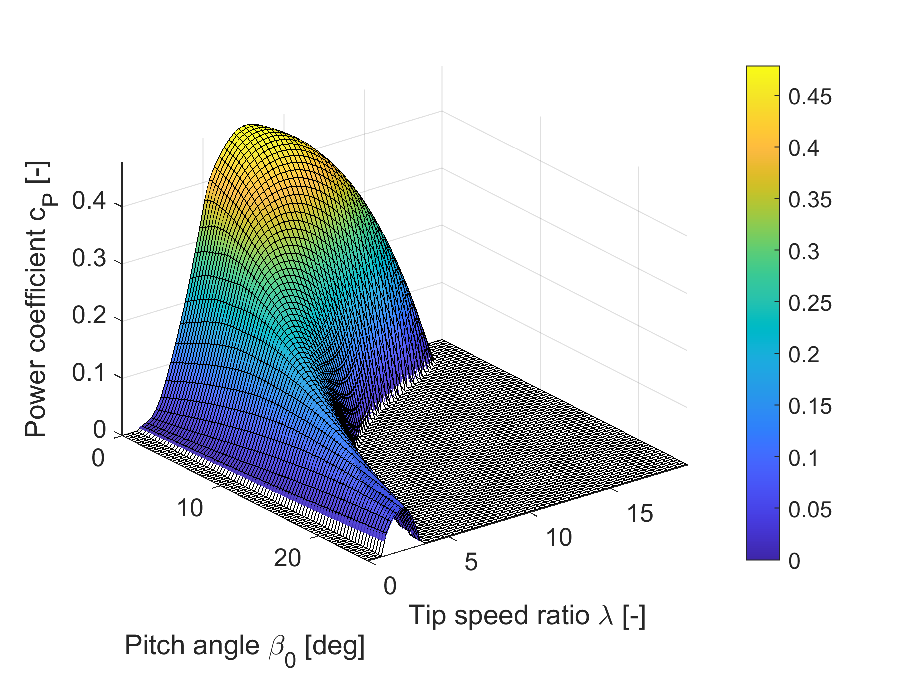
\includegraphics[width=0.49\textwidth]{figures/figDirECC21/Cp_NRRLFAST5MW.eps}
    }\hfill
    \subfloat[Torque coefficient $c_Q$]{%
        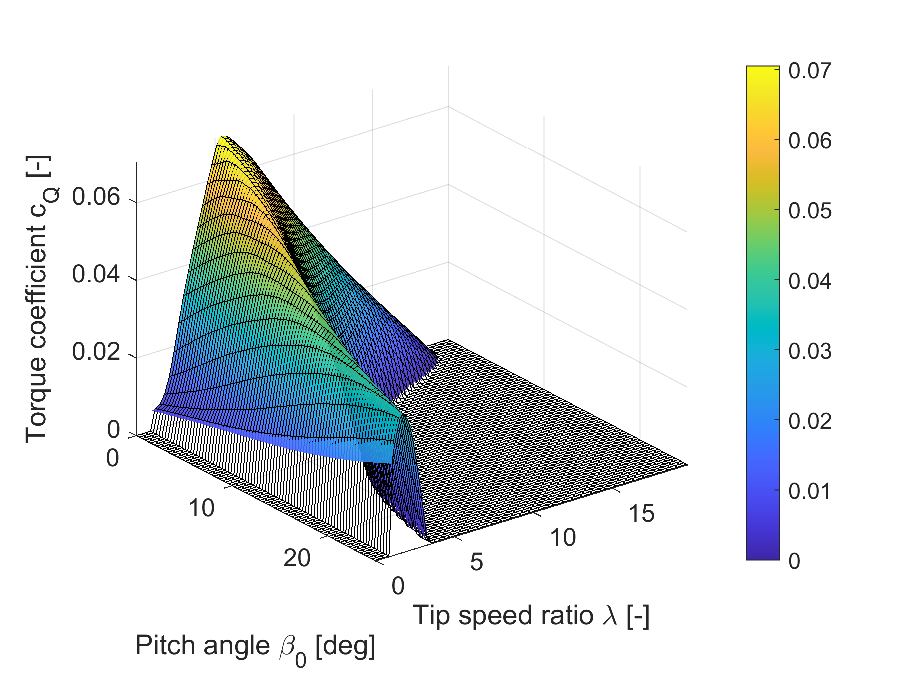
\includegraphics[width=0.49\textwidth]{figures/figDirECC21/Cq_NRRLFAST5MW.eps}
    }\\[1ex]
    \subfloat[Thrust coefficient $c_T$]{%
        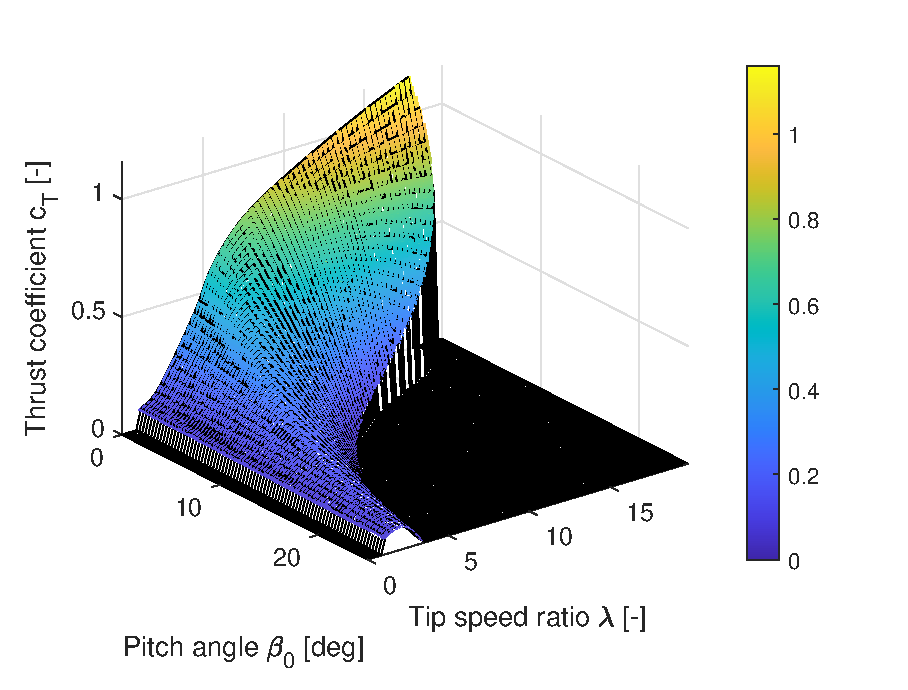
\includegraphics[width=0.49\textwidth]{figures/figDirECC21/Ct_NRRLFAST5MW.eps}
    }
    \caption{Aerodynamic power, torque and thrust coefficient surfaces with respect to blade pitch angle and tip-speed ratio for the NREL 5MW model.} % Lookup tables of power, torque and thrust coefficients with respect to blade pitch angle and tip speed ratio for the NREL 5MW model
    \label{fig:CPCT}
\end{figure}
%
\subsection{Structural Models} \label{subsec:Structural Models}
In this section, two modeling approaches are presented. They are based on previous studies that derive structural models \cite{schlipf2013nonlinear, mulders2020preventing, Bianchi2007} and are modified and extended to be amenable to comparison and systematic verification with FAST. Both models leverage the aerodynamic model from Equation~\eqref{eq:aero}. The resulting nonlinear differential equations were implemented in Simulink, parameterized using the NREL 5MW turbine parameters given in Table \ref{table:1}, and compared in closed-loop simulations with FAST simulations.
%
\subsubsection{Model 1: Structural Model with Tower Fore-Aft and Side-to-Side Motion}

Models for controller design only need to capture the main dynamics of a system. Hence, the first model uses only the rotor speed, tower displacements and velocities as states. Based on the equations given above, the relationship between the forces and moments acting on the turbine, the inputs, and the rotor speed and tower movements, the states, can be expressed as
\begin{equation}\label{eq:Mdl1NonLin}
    \begin{split} 
        \dot{\omega}_r(t) &= \frac{1}{J_r + N_g^2 J_g}(T_r(t) - N_{g}T_{g}(t)) = \frac{1}{J_s}(T_r(t) - N_{g}T_{g}(t)),   \\
        \ddot{x}_{t}(t) & = \frac{1}{m_{t}}(-B_{t}\dot{x}_{t}(t) - K_{t}{x}_{t}(t) + F_{T,r}(t)), \\
        \ddot{y}_{t}(t) &= \frac{1}{m_{t}}(-B_{t,\text{sw}} \dot{y}_{t}(t) - K_{t,\text{sw}}{y}_{t}(t) + F_{T,y}(t)),       
    \end{split}
\end{equation}
where $\omega_r$ is the rotor speed and $x_t$ and $y_t$ represent the fore-aft and side-to-side tower displacements, respectively. The calculation of the side-to-side force acting on the nacelle as a function of the rotor and generator torques is detailed below. The transmission inertia $J_s$ is the combined inertia of the rotor and the generator, see Equation~\eqref{eq:Tr1_background}. The values for the modal tower mass $m_{t}$, fore-aft and side-to-side damping and stiffness terms $B_t$, $B_{t,\text{sw}}$, $K_t$ and $K_{t,\text{sw}}$, and hub height $H_t$ are provided in Table~\ref{table:1}. They are derived from the documentation of the NREL 5MW reference turbine \cite{jonkman2009definition}.

The side-to-side force is caused by the torsional nacelle moment $M_x$:
\begin{equation}
    F_{T,y}(t) = -\frac{3}{2H_t}M_x(t).
\end{equation}
The lumped force is obtained analogously to the fore-aft force in \cite{Bianchi2007}, with the factor $3/(2H_t)$ following from cantilever theory \cite{selvam2009feedback}. The reasoning is as follows: the moment $M_x$ acts on the nacelle at hub height $H_t$. The tower can be regarded as a cantilever beam fixed at the base, with its free end located at hub height. Since the qLPV model captures the tower as a single-degree-of-freedom system represented by the hub-height displacement $y_t$, the equivalent lumped force $F_{T,y}$ is obtained by requiring it to produce the same tip deflection as the applied moment. For a cantilever of length $H_t$, a tip moment $M_x$ produces a tip deflection of $M_x H_t^2/(2EI)$, while a tip point force $F_{T,y}$ produces a tip deflection of $F_{T,y} H_t^3/(3EI)$, where $E$ is the modulus of elasticity of the tower material and $I$ is the second moment of area of the tower cross-section. Setting the two equal gives $|F_{T,y}|\,(2/3)\,H_t = |M_x|$. The negative sign results from the definition of $y_t$ pointing to the left when looking downwind: a moment $M_x$ in the direction of rotor rotation deflects the tower top in the negative $y_t$-direction.

The moment $M_x$ is the sum of the generator torque and the reaction moment at the gearbox housing around the fore-aft axis. The latter is the difference between the low-speed shaft torque and the high-speed shaft torque. Assuming an ideal, massless gearbox and a generator rotating in the same direction as the rotor, the moment balance yields
\begin{align*}
    M_x(t) = T_{\text{lss}}(t) - T_{\text{hss}}(t) + T_g(t).
\end{align*}
With the generator equation and the rotor equation from the equation set~\eqref{eq:DrvTr} as well as the rigid-drivetrain assumption $\dot{\omega}_g = N_g\dot{\omega}_r$, the moment $M_x$ can be expressed in terms of the rotor torque and the rotor acceleration as
\begin{align*}
    M_x(t) &= T_{\text{lss}}(t) - J_g\dot{\omega}_g(t)\\
    &= T_r(t) - J_r\dot{\omega}_r(t) - J_g\dot{\omega}_g(t)\\
    &= T_r(t) - \left(J_r + N_g J_g\right)\dot{\omega}_r(t).
\end{align*}
This moment is hence the aerodynamic torque minus the rate of change of the angular momentum of the rotating parts. Note that the generator inertia enters with $N_g J_g$ and not with the reflected inertia $N_g^2 J_g$ contained in $J_s$. Replacing the change in rotor speed with $\dot{\omega}_r = (T_r - N_g T_g)/J_s$ yields
\begin{align}\label{eq:Mx}
    M_x(t) = (1-c_{M_x})\,T_r(t) + c_{M_x}N_g T_g(t), \qquad c_{M_x} = \frac{J_r + N_g J_g}{J_r + N_g^2 J_g},
\end{align}
with a resulting coefficient         $c_{M_x} \approx 0.877$ for the NREL 5MW turbine. In steady state, where $T_r = N_gT_g$ and $\dot{\omega}_r = 0$ hold, the moment $M_x$ equals the rotor torque $T_r$.

While the fore-aft lumped-force model is established in the literature \cite{Bianchi2007}, the side-to-side counterpart presented here is, to the best of the author's knowledge, original. The validity of this simplified assumption is confirmed against linearized FAST models in Section~\ref{subsec:ResultsqLPVModel}, where the side-to-side tower response is shown to capture the first tower mode frequency of the FAST reference, see Figures~\ref{fig:Bode4} and~\ref{fig:Bode12}, and to reproduce the side-to-side acceleration amplitudes in the closed-loop wind sweep reasonably well, see Figure~\ref{fig:TimeCmpMdlSweep}.

The tower modal mass \( m_t \) is calculated from the total tower weight \( m_{\text{tower}} \), the total nacelle weight \( m_{\text{nacelle}} \), the total hub weight \( m_{\text{hub}} \), and the total blade weight \( m_{\text{blade}} \) as  
\begin{align} \label{eq:modalMass}
    m_t = \frac{1}{4}m_{\text{tower}} + m_{\text{nacelle}} + m_{\text{hub}} + n_b m_{\text{blade}}.
\end{align} 
This is the same calculation of the modal mass as suggested in \cite{schlipf2013nonlinear}.
The fore-aft stiffness and damping $K_t$ and $B_t$ are calculated from the corresponding eigenfrequencies $f_{t,\text{fa}}$ and  $f_{t,\text{sw}}$ and damping $\zeta_t$  with the fore-aft terms as
\begin{align} \label{eq:DampingStiffness}
    K_t = (2\pi f_{t,\text{fa}})^2 m_t\quad\text{and}\quad B_t = 2 \zeta_t (2\pi f_{t,\text{fa}}) m_t,
\end{align}
and the side-to-side terms $K_{t,\text{sw}}$ and $B_{t,\text{sw}}$ derived identically based on $f_{t,\text{sw}}$.
Table~\ref{table:1} also includes the gearbox ratio $N_g$ and the rotor inertia $J_r$, which consists of the hub inertia and the combined blade inertia of all blades. It is assumed that both $F_{T,r}$ and $T_r$ represent the force and torque acting at the nacelle, implicitly accounting for the forces from all three blades. The vectors for the inputs and states of the linear first- and second-order differential equations from the equation set~\eqref{eq:Mdl1NonLin} are defined as:
\begin{equation}\label{eq:NonLinInputDef}
    \begin{split}
        \bm{w} &= [F_{T,r} \quad T_r \quad T_g ]^T  \in \mathbb{R}^{3 \times 1},\\
        \bm{x}_{\text{Mdl1}} &= [ x_{t} \quad y_{t} \quad \dot{x}_{t} \quad \dot{y}_{t} \quad \omega_r]^T \in \mathbb{R}^{5 \times 1}.
    \end{split}
\end{equation}
The control inputs of the model are the reference torque and pitch, with the wind acting as a disturbance. This model does not include the dynamics between the reference generator torque and blade pitch, $T_{g,\text{ref}}$ and $\beta_{0,\text{ref}}$, and the actual inputs $T_{g}$ and $\beta_{0}$. Therefore, the first-order actuator dynamics from Equations~\eqref{eq:Tact} and~\eqref{eq:betaact} need to be concatenated with the turbine dynamics in the simulation. Thus, the turbine inputs are the actuator outputs and the wind 
\begin{align} \label{eq:CtrlInputDef}
    \bm{w}_{\text{Mdl}} &= [ V_{\infty} \quad T_{g} \quad \beta_{0}]^T \in \mathbb{R}^{3 \times 1},
\end{align}
where the freestream wind $V_{\infty}$ and the effective wind speed $V_r$ differ by the tower movement, i.e., $V_r = V_{\infty} - \dot{x}_t$.
The gradients of the aerodynamic thrust and torque at an operating point need to be calculated to derive a model using the real inputs provided in the vector $\bm{w}_{\text{Mdl}}$ instead of the fictitious ones in vector $\bm{w}$. The variations of thrust and torque around an operating point depend on changes in the effective wind speed $V_r$, and hence in the disturbance input $V_{\infty}$ and the state $\dot{x}_t$, as well as on changes in the state $\omega_r$ and the control input $\beta_{0}$:
\begin{equation} \label{eq:FTTRGrad}
    \begin{split}
        \hat{F}_{T,r}(t) &= k_{F_T,V} \left( \hat{V}_{\infty}(t) - \hat{\dot{x}}_{t}(t)\right) + \; B_{F_T} \hat{\omega_r}(t) +  k_{F_T,\beta} \hat{\beta_0}(t), \\
        \hat{T}_r(t) &= k_{T_r,V} \left( \hat{V}_{\infty}(t) - \hat{\dot{x}}_{t}(t)\right) + B_{T_r} \hat{\omega_r}(t) + k_{T_r,\beta} \hat{\beta_0}(t),
    \end{split}
\end{equation} \enlargethispage{\baselineskip}
with a hat denoting a variation with respect to a steady state. Substituting the terms from Equations~\eqref{eq:FTTRGrad} into Equations~\eqref{eq:Mdl1NonLin} yields a linear model describing the influence of changes in the inputs $\bm{w}_{\text{Mdl}}$ on the states $\bm{x}_{\text{Mdl1}}$ from Equations~\eqref{eq:NonLinInputDef} and~\eqref{eq:CtrlInputDef}. The partial derivatives of the rotor thrust force and torque are calculated from the equation set~\eqref{eq:aero} with $[F_{T,r} \quad T_r] = [k_{c_T} c_T(\lambda,\beta_0) V_r^2 \quad k_{c_Q}  c_Q(\lambda,\beta_0) V_r^2]$ where the constants are $k_{c_T} = 0.5 \rho_a A_r$ and $k_{c_Q} = 0.5 \rho_a R_r A_r$, respectively. This results in the derivatives: 
\begin{align*}
    k_{F_T,V} = \frac{\partial F_{T,r}(t)}{\partial{V_{\infty}(t)}} \bigg|_{\bar{V}_{\infty},\bar{\omega}_r,\bar{\beta}_0} &= k_{c_T}  \bar{V}_{\infty} \left(2\bar{c}_T + \frac{\partial  c_T(\lambda,\beta_0)}{\partial{\lambda(t)}}\bigg|_{\bar{V}_{\infty},\bar{\omega}_r,\bar{\beta}_0}  \frac{ \partial \lambda(t)}{ \partial V_{\infty}(t)}\bigg|_{\bar{V}_{\infty},\bar{\omega}_r,\bar{\beta}_0} \bar{V}_{\infty} \right),\\
    %
    B_{F_T} = \frac{\partial F_{T,r}(t)}{\partial{\omega_r(t) }}  \bigg|_{\bar{V}_{\infty},\bar{\omega}_r,\bar{\beta}_0} &= 
    k_{c_T} \frac{\partial c_{T}(\lambda,\beta_0)}{\partial \lambda(t)} \bigg|_{\bar{V}_{\infty},\bar{\omega}_r,\bar{\beta}_0} \frac{ \partial \lambda(t)}{ \partial \omega_r(t)}\bigg|_{\bar{V}_{\infty},\bar{\omega}_r,\bar{\beta}_0} \bar{V}_{\infty}^2, \\
    %
    k_{F_T,\beta} = \frac{\partial F_{T,r}(t)}{\partial{\beta_0(t) }}  \bigg|_{\bar{V}_{\infty},\bar{\omega}_r,\bar{\beta}_0} &= 
    k_{c_T} \frac{\partial c_{T}(\lambda,\beta_0)}{\partial \beta_0(t)} \bigg|_{\bar{V}_{\infty},\bar{\omega}_r,\bar{\beta}_0} \bar{V}_{\infty}^2, \\
    %
    k_{T_r,V} = \frac{\partial T_{r}(t)}{\partial{V_{\infty}(t)}} \bigg|_{\bar{V}_{\infty},\bar{\omega}_r,\bar{\beta}_0} &= k_{c_Q}  \bar{V}_{\infty} \left(2\bar{c}_Q + \frac{\partial  c_Q(\lambda,\beta_0)}{\partial{\lambda(t)}}\bigg|_{\bar{V}_{\infty},\bar{\omega}_r,\bar{\beta}_0}  \frac{ \partial \lambda(t)}{ \partial V_{\infty}(t)}\bigg|_{\bar{V}_{\infty},\bar{\omega}_r,\bar{\beta}_0} \bar{V}_{\infty} \right),\\
    %
    B_{T_r} = \frac{\partial T_{r}(t)}{\partial{\omega_r(t) }}  \bigg|_{\bar{V}_{\infty},\bar{\omega}_r,\bar{\beta}_0} &= 
    k_{c_Q} \frac{\partial c_{Q}(\lambda,\beta_0)}{\partial \lambda(t)} \bigg|_{\bar{V}_{\infty},\bar{\omega}_r,\bar{\beta}_0} \frac{ \partial \lambda(t)}{ \partial \omega_r(t)}\bigg|_{\bar{V}_{\infty},\bar{\omega}_r,\bar{\beta}_0} \bar{V}_{\infty}^2, \\
    %
    k_{T_r,\beta} = \frac{\partial T_{r}(t)}{\partial{\beta_0(t) }}  \bigg|_{\bar{V}_{\infty},\bar{\omega}_r,\bar{\beta}_0} &= 
    k_{c_Q} \frac{\partial c_{Q}(\lambda,\beta_0)}{\partial \beta_0(t)} \bigg|_{\bar{V}_{\infty},\bar{\omega}_r,\bar{\beta}_0} \bar{V}_{\infty}^2, 
\end{align*}
with a bar over a variable denoting a steady-state value at an operating point.
These derivatives are used to implement the qLPV models in this section and the partial derivatives of the torque are used in the qLMPC controller design in Chapter \ref{sec:Application to Wind Turbine Control4}. The derivatives of the tip-speed ratio are calculated as
\begin{align*}
    \frac{ \partial \lambda(t)}{\partial V_{\infty}(t)}\bigg|_{\bar{V}_{\infty},\bar{\omega}_r,\bar{\beta}_0} &= - \frac{\omega_r(t) R_r}{(V_{\infty}(t)-\dot{x}_t(t))^2}\bigg|_{\bar{V}_{\infty},\bar{\omega}_r,\bar{\beta}_0} = - \frac{\bar{\omega_r}R_r}{\bar{V}_{\infty}^2},\\
    \frac{ \partial \lambda(t)}{\partial \omega_{r}(t)}\bigg|_{\bar{V}_{\infty},\bar{\omega}_r,\bar{\beta}_0} &=  \frac{ R_r}{(V_{\infty}(t)-\dot{x}_t(t))}\bigg|_{\bar{V}_{\infty},\bar{\omega}_r,\bar{\beta}_0} = \frac{R_r}{\bar{V}_{\infty}},
\end{align*}
and the values and derivatives of the thrust and torque coefficients are deduced from the calculated lookup tables depicted in Figure \ref{fig:CPCT}.
The system and input matrices are

\begin{align*}
    \bm{A}_{\text{Mdl1}} &= \begin{bmatrix}
        0 & 0 & 1 & 0 & 0 \\
        0 & 0 & 0 & 1 & 0 \\
        - \frac{K_t}{m_t} & 0 & -\frac{B_t+ k_{F_T,V}(\bm{\rho}_{\Rho})}{m_t} & 0 & \frac{B_{F_T}(\bm{\rho}_{\Rho})}{m_t} \\
        0 &  - \frac{K_{t,\text{sw}}}{m_t}  & \frac{3(1-c_{M_x})k_{T_r,V}(\bm{\rho}_{\Rho})}{2 m_t H_t} & - \frac{B_{t,\text{sw}}}{m_t} & -\frac{3(1-c_{M_x})B_{T_r}(\bm{\rho}_{\Rho})}{2 m_t H_t} \\
        0 & 0 & - \frac{k_{T_r,V}(\bm{\rho}_{\Rho})}{J_s} & 0 & \frac{B_{T_r}(\bm{\rho}_{\Rho})}{J_s}
    \end{bmatrix}  \in \mathbb{R}^{5 \times 5},\\
    \bm{B}_{\text{Mdl1}} &= \begin{bmatrix}
        0 & 0 & 0 \\
        0 & 0 & 0 \\
        \frac{k_{F_T,V}(\bm{\rho}_{\Rho})}{m_t} & 0 & \frac{k_{F_T,\beta}(\bm{\rho}_{\Rho})}{m_t} \\
        -\frac{3(1-c_{M_x})k_{T_r,V}(\bm{\rho}_{\Rho})}{2 m_t H_t} & -\frac{3 c_{M_x} N_g}{2 m_t H_t} &  -\frac{3(1-c_{M_x})k_{T_r,\beta}(\bm{\rho}_{\Rho})}{2 m_t H_t}\\
        \frac{k_{T_r,V}(\bm{\rho}_{\Rho})}{J_s} & -\frac{N_g}{J_s} &  \frac{k_{T_r,\beta}(\bm{\rho}_{\Rho})}{J_s}
    \end{bmatrix}  \in \mathbb{R}^{5 \times 3}
\end{align*} \enlargethispage{\baselineskip}
with the scheduling parameter vector $\bm{\rho}_{\Rho} = \left[V_{\infty}\quad \beta_0 \quad \omega_r\right]$. The turbine parameters used for this model are those of the NREL 5MW reference turbine, as implemented in FAST v8.16 \cite{jonkman2016fast}. 
%
This 5th-order model is compared to FAST models linearized at different freestream wind speeds in the frequency domain for a frequency range relevant for wind turbines. The above-described nonlinear dynamics are implemented in Simulink; both the FAST S-function and the Simulink implementation are run in closed loop with a baseline PI controller. The results are compared with a closed-loop FAST model to verify the Simulink model. Actuator dynamics for torque and pitch are included in the simulation as a separate Simulink model.
%
This relatively simple model Mdl1 provides a reasonable approximation of the FAST NREL 5MW model. Nevertheless, it is investigated whether a slightly more involved approach, also taking the generator and blade dynamics into account, would improve the fit to FAST in an open-loop verification.

\subsubsection{Model 2: Structural Model with Tower and Blade Out-of-Plane Motion} 
A similar but more detailed modeling approach, inspired by \cite{Bianchi2007}, is presented here. The method proposed in that book is extended by including the side-to-side tower displacement $y_t$, and modified so that the qLPV model inputs correspond to the actual turbine control inputs, enabling direct comparison with FAST. Lagrange's equation is used to build a model with rotor and generator speed, tower, and blade displacement as the states. This approach is therefore an extension of the simpler model considered above. The notation below follows \cite{Bianchi2007} where possible.
%
A mechanical system of arbitrary complexity can be described by the fundamental equation of motion:
\begin{align} \label{eqLagrange}
    \mathbf{M}\ddot{\bm{q}}(t) + \mathbf{C}\dot{\bm{q}}(t) + \mathbf{K}{\bm{q}}(t) = \mathbf{Q}(\dot{\bm{q}}(t), \bm{q}(t), t, \bm{w}(t)),
\end{align}
where $\mathbf{M}$, $\mathbf{C}$, and $\mathbf{K}$ are the mass, damping, and stiffness matrices, $\bm{q}$ represents the system states, $\bm{w}$ denotes the system inputs, and $\mathbf{Q}$ is a vector of generalized forces. For mechanical structures with any number of degrees of freedom, Lagrange's equation for the $i$-th component of \(\bm{q}\) and \(\mathbf{Q}\) is expressed as
\begin{align*}
    \frac{d}{dt} \left(\frac{\partial E_k(t)}{\partial \dot{q}_i(t)} \right) - \frac{\partial E_k(t)}{\partial q_i(t)} + \frac{\partial E_d(t)}{\partial \dot{q}_i(t)} + \frac{\partial E_p(t)}{\partial q_i(t)} = Q_i(t),
\end{align*}
where \(E_k\) and \(E_p\) are the kinetic and potential energies, respectively, and $\partial E_d(t)/\partial \dot{q}_i(t)$ incorporates the damping forces through Rayleigh's dissipation function $E_d$. For simplicity, the term $E_d$ is referred to as dissipative energy in the later part of this thesis. %\footnote{ While \(E_d\) is labeled similarly to an energy term, it does not represent stored energy in the traditional Lagrangian sense.  The derivative \(\partial E_d / \partial \dot{q}_i\) yields the damping force associated with coordinate \(q_i\).}. %Rather, it serves the role of a dissipation function, equivalent in form and function to Rayleigh's dissipation function \(D(\dot{\bm{q}})\), but denoted here as \(E_d\) to avoid conflicts with other uses of the symbol \(D\) in this work.
%
These terms can be described as
\begin{align*}
    E_k(t) & = \frac{1}{2}\left(m_{t,\text{fa}}\dot{x}_t(t)^2 + n_b m_b(r_b\dot{\delta}_b(t) + \dot{x}_t(t))^2 + m_t\dot{y}_t(t)^2 + J_r\omega_r(t)^2 + J_{gr}\omega_{gr}(t)^2\right),\\
    E_d(t)  & = \frac{1}{2}\left(B_t\dot{x}_t(t)^2 + n_b B_b(r_b\dot{\delta}_b(t))^2 + B_{t,\text{sw}}\dot{y}_t(t)^2 + B_{sr}(\omega_r(t) - \omega_{gr}(t))^2\right),\\
    E_p(t)  & = \frac{1}{2}\left(K_t{x}_t(t)^2 + n_b K_b(r_b{\delta}_b(t))^2 + K_{t,\text{sw}}{y}_t(t)^2 + K_{sr}(\theta_r(t) - \theta_{gr}(t))^2\right),
\end{align*}
with tower displacements \(x_t\) and \(y_t\) defined as above\footnote{Note that the terms \(E_k\) and \(E_p\) represent energies in the unit Joules, but \(E_d\) corresponds to a dissipation function representing power in the unit Watts. The coefficients \(B_t\), \(B_b\), and \(B_{t,\text{sw}}\) are linear damping coefficients with units of~\(\text{kg}/\text{s}\), representing force per linear velocity. The rotational damping coefficient \(B_{sr}\) has units of \(\text{kg}\cdot \text{m}^2/\text{s}\), representing torque per angular velocity. The linear stiffness coefficients \(K_t\), \(K_b\), and \(K_{t,\text{sw}}\) have units of \(\text{N}/\text{m}\) (equivalently \(\text{kg}/\text{s}^2\)), and the torsional stiffness coefficient \(K_{sr}\) has units of \(\text{N}\cdot\text{m}/\text{rad}\). Since radians are dimensionless in SI, the product \(K_{sr}(\theta_r - \theta_{gr})^2\) has units of energy, \( \text{N}\cdot\text{m} =\text{kg} \cdot \text{m}^2 / \text{s}^2\).}. The fore-aft modal tower mass without the blades is $m_{t,\text{fa}} = m_t - n_b m_{\text{blade}}$, since the blades are accounted for separately by their modal mass $m_b$. The number of blades is $n_b=3$, \(\delta_b\) the out-of-plane blade angle, $r_b$ the radial distance between rotor hub and the application point of the lumped aerodynamic force, and \(\theta_r\), \(\omega_r\), \(\theta_{gr}\), and \(\omega_{gr}\) the rotor and generator angles and angular speeds, all measured on the low-speed shaft rotor side.

The relationships between the generator angle and speed on the low-speed shaft rotor side and those on the high-speed shaft generator side are $\theta_{gr} = \theta_{g}/N_g$ and  $\omega_{gr} = \omega_{g}/N_g$. The modal blade mass $m_b = 1/4\; m_{\text{blade}}$ is calculated from the blade weight $m_{\text{blade}}$. The factor of 1/4 is used in this thesis, as it is commonly utilized as an approximation for the modal mass of a uniform cantilever beam when considering its first bending mode. Note that this is also the motivation for applying this factor for calculating the modal tower mass $m_t$, see Equation~\eqref{eq:modalMass}. Moreover, this approximated modal mass provides a good fit to the linearized FAST models around the first flapwise frequency of approximately 0.7\,Hz. 

The damping and stiffness of the blade, $B_b$ and $K_b$, are derived from the blade eigenfrequency as described in Equation~\eqref{eq:DampingStiffness}. %
The inertias of the rotor \(J_r\) and the generator \(J_{gr}\) are linked by the gearbox ratio \(N_g\), as is the generator torque \(T_g\):
\begin{align*}
    \theta_{gr}(t) = \frac{\theta_{g}(t)}{N_g}, \quad J_{gr} = J_{g}{N_g}^2,  \quad T_{gr}(t) = T_{g}(t)N_g. 
\end{align*}
Since the drivetrain damping and stiffness are already provided by FAST on the low-speed shaft side, the parameters are simply renamed to 
$B_{sr} = B_{s}$ and  $K_{sr} = K_{s}$ for consistency.

%
Assuming that the force \(F_{T,r}\) is the total force acting on the nacelle, summing up all the forces acting on the blades, $T_r$ the resulting aerodynamic rotor moment, and $T_{gr} = N_g T_g$ the generator moment on the rotor side, i.e., the low-speed shaft side, the model state \(\bm{q}\) and the generalized force vector \(\mathbf{Q}\) from Equation~\eqref{eqLagrange} are:
\begin{align*}
    \bm{q}& = [x_t \quad \delta_b \quad y_t \quad \theta_r \quad \theta_{gr}]^T  \in \mathbb{R}^{5 \times 1},\\
    \mathbf{Q} & = [n_b F_{T,b} \quad n_b F_{T,b}r_b \quad F_{T,y} \quad T_r \quad -T_{gr}]^T \in \mathbb{R}^{5 \times 1}\\
    & = \left[F_{T,r} \quad r_bF_{T,r} \quad -\tfrac{3}{2H_t}M_x\quad T_r \quad -N_g T_g\right]^T,
\end{align*}
where the blade modal mass $m_b$ is assumed to be located at the application point of the lumped aerodynamic force at radius $r_b$. For the side-to-side excitation, the torsional nacelle moment $M_x$ is approximated by its rigid-drivetrain form from Equation~\eqref{eq:Mx}, which is valid below the drivetrain torsional mode at approximately 2.2\,Hz in Mdl2 (approximately 1.6\,Hz in FAST, with flexible blades and tower).
%For the flexible drivetrain, the torsional nacelle moment follows from the low-speed shaft torque as
%$\begin{align*}
    %    M_x = \left(1 - \frac{1}{N_g}\right)\left(K_s(\theta_r - \theta_{gr}) + B_s(\dot{\theta}_r - \dot{\theta}_{gr})\right) + T_g,
    %\end{align*}
    %see Equation~\eqref{eq:Mx} for the rigid case. This moment is added as an external excitation.
    
    The time derivatives of the partial derivatives of the kinetic energy yield the inertia terms $\mathbf{M}_5\ddot{\bm{q}}$:
    % For \( F_T \) see page 34 Bianchi Fig 3.4
    \begin{align*}
        \frac{d}{dt} \left(\frac{\partial E_k(t)}{\partial \dot{x}_t(t)} \right) &= m_{t,\text{fa}}\ddot{x}_t(t) + n_b m_b(r_b\ddot{\delta}_b(t) + \ddot{x}_t(t)), \\
        \frac{d}{dt} \left(\frac{\partial E_k(t)}{\partial \dot{\delta}_b(t)} \right) &= n_b m_b(r_b^2\ddot{\delta}_b(t) + r_b\ddot{x}_t(t)), \\
        \frac{d}{dt} \left(\frac{\partial E_k(t)}{\partial \dot{y}_t(t)} \right) &= m_t\ddot{y}_t(t), \\
        \frac{d}{dt} \left(\frac{\partial E_k(t)}{\partial \dot{\theta}_r(t)} \right) &= J_r\ddot{\theta}_r(t), \\
        \frac{d}{dt} \left(\frac{\partial E_k(t)}{\partial \dot{\theta}_{gr}(t)} \right) &= J_{gr}\ddot{\theta}_{gr}(t),
    \end{align*}
    with the generator inertia referred to the low-speed shaft $J_{gr} = N_g^2 J_g$ and the fore-aft modal mass $m_{t,\text{fa}} = m_t - n_b m_{\text{blade}}$, since the blade mass is accounted for separately by the flap degree of freedom. This results in the mass matrix
    \[
    \mathbf{M}_5 = \begin{bmatrix}
        m_{t,\text{fa}} + n_b m_b & n_b m_b r_b & 0 & 0 & 0 \\
        n_b m_b r_b & n_b m_b r_b^2 & 0 & 0 & 0 \\
        0 & 0 & m_t & 0 & 0 \\
        0 & 0 & 0 & J_r & 0 \\
        0 & 0 & 0 & 0 & J_{gr}
    \end{bmatrix}  \in \mathbb{R}^{5 \times 5}.
    \]
    %
    The kinetic energy $E_k$ does not depend explicitly on the generalized coordinates $q_i$, so that
    \begin{align*}
        \frac{\partial E_k}{\partial q_i }= 0\quad \forall i = 1, 2, 3, 4, 5.
    \end{align*}
    The influence of the first derivative of the dissipative energy is:
    \begin{align*}
        \frac{\partial E_d(t)}{\partial \dot{x}_t(t) } &= B_t \dot{x}_t(t), \\
        \frac{\partial E_d(t)}{\partial \dot{\delta}_b(t) } &= n_b B_b(r_b \dot{\delta}_b(t)) r_b, \\
        \frac{\partial E_d(t)}{\partial \dot{y}_t(t) } &= B_{t,\text{sw}} \dot{y}_t(t), \\
        \frac{\partial E_d(t)}{\partial \dot{\theta}_r(t) } &= B_{sr}(\omega_r(t) - \omega_{gr}(t)), \\
        \frac{\partial E_d(t)}{\partial \dot{\theta}_{gr}(t) } &= -B_{sr}(\omega_r(t) - \omega_{gr}(t)),
    \end{align*}
    with the resulting matrix \( \mathbf{C}_5 \):
    \[
    \mathbf{C}_5 = \begin{bmatrix}
        B_t & 0 & 0 & 0 & 0 \\
        0 & n_b B_b r_b^2 & 0 & 0 & 0 \\
        0 & 0 & B_{t,\text{sw}} & 0 & 0 \\
        0 & 0 & 0 & B_{sr} & -B_{sr} \\
        0 & 0 & 0 & -B_{sr} & B_{sr}
    \end{bmatrix}  \in \mathbb{R}^{5 \times 5}.
    \]
    %   
    Finally, the influence from the potential energy is
    \begin{align*}
        \frac{\partial E_p(t)}{\partial x_t(t) } &= K_t x_t(t), \\
        \frac{\partial E_p(t)}{\partial \delta_b(t) } &= n_b K_b(r_b \delta_b(t)) r_b, \\
        \frac{\partial E_p(t)}{\partial y_t(t) } &= K_{t,\text{sw}} y_t(t), \\
        \frac{\partial E_p(t)}{\partial \theta_r(t) } &= K_{sr}(\theta_r(t) - \theta_{gr}(t)), \\
        \frac{\partial E_p(t)}{\partial \theta_{gr}(t) } &= -K_{sr}(\theta_r(t) - \theta_{gr}(t)),
    \end{align*}
    resulting in matrix \(\mathbf{K}_5\):
    \[
    \mathbf{K}_5 = \begin{bmatrix}
        K_t & 0 & 0 & 0 & 0 \\
        0 & n_b K_b r_b^2 & 0 & 0 & 0 \\
        0 & 0 & K_{t,\text{sw}} & 0 & 0 \\
        0 & 0 & 0 & K_{sr} & -K_{sr} \\
        0 & 0 & 0 & -K_{sr} & K_{sr}
    \end{bmatrix}  \in \mathbb{R}^{5 \times 5}.
    \]
    With the force input vector \(\bm{w}=  [F_{T,r} \quad T_r \quad T_{g} ]^T\) the scaling matrix \(\mathbf{Q}_{5\times3}\) is
    \[
    \mathbf{Q}_{5\times3} = \begin{bmatrix}
        1 & 0 & 0  \\
        r_b & 0 & 0  \\
        0 & -\frac{3(1-c_{M_x})}{2H_t} & -\frac{3c_{M_x}N_g}{2H_t}\\
        0 & 1 & 0 \\
        0 & 0 & -N_g
    \end{bmatrix} \in \mathbb{R}^{5 \times 3}.
    \]
    %
    A state vector is typically constructed from the concatenation of the vector \(\bm{q}\) and its derivative \(\dot{\bm{q}}\). However, in the case of the considered wind turbine model, the slip angle \(\theta_s\) is introduced for numerical stability. It is defined as the difference between the rotor and generator angles, \(\theta_r\) and \(\theta_{gr}\), respectively, resulting in the following nine states:
    \begin{align}\label{eq:X7}
        \bm{x}_{\text{Mdl2}} = [\underbrace{x_t \quad \delta_b \quad y_t \quad \theta_s}_{\tilde{\bm{q}}}   \quad \underbrace{\dot{x}_t \quad \dot{\delta}_b \quad \dot{y}_t  \quad {\omega}_r \quad {\omega}_{gr}}_{\dot{\bm{q}}}  ]^T \in \mathbb{R}^{9 \times 1},
    \end{align} 
    which necessitates the introduction of the altered stiffness matrix \(\tilde{\mathbf{K}}_{5 \times 4} \in \mathbb{R}^{5 \times 4}\), comprising the first four columns of the matrix \(\mathbf{K}_{5}\). The resulting 9th-order state-space model with input \(\bm{w}\) and states \(\bm{x}_{\text{Mdl2}}\) from Equation~\eqref{eq:X7} is:
    \begin{align}\label{eq:7state}
        \dot{\bm{x}}_{\text{Mdl2}}(t) = \underbrace{\begin{bmatrix}
                \bm{0}_{4 \times 4} & \mathbf{L}_{4 \times 5}  \\
                -\mathbf{M}_5^{-1}\tilde{\mathbf{K}}_{5 \times 4} & -\mathbf{M}_5^{-1}\mathbf{C}_5
        \end{bmatrix}}_{\bm{A}_{\text{Mdl2}}  \in \mathbb{R}^{9 \times 9}} \bm{x}_{\text{Mdl2}}(t) + \underbrace{\begin{bmatrix}
                \bm{0}_{4 \times 3} \\
                \mathbf{M}_5^{-1}\mathbf{Q}_{5 \times 3}
        \end{bmatrix}}_{\bm{B}_{\text{linMdl2}}  \in \mathbb{R}^{9 \times 3}} \bm{w}(t),  
    \end{align}
    with 
    \[
    \mathbf{L}_{4 \times5} = \begin{bmatrix}
        1 & 0 & 0 & 0 & 0 \\
        0 & 1 & 0 & 0 & 0 \\
        0 & 0 & 1 & 0 & 0 \\
        0 & 0 & 0 & 1 & -1
    \end{bmatrix} \in \mathbb{R}^{4 \times 5}.
    \]
    %
    Note that the model is linear in the input $\bm{w} = [F_{T,r} \quad T_r \quad T_g]^T$ from Equation~\eqref{eq:NonLinInputDef}, which contains the aerodynamic force and torque as fictitious inputs. In contrast, the vector $\bm{w}_{\text{Mdl}}$ from Equation~\eqref{eq:CtrlInputDef} contains the true turbine inputs, i.e., the freestream wind speed, the generator torque, and the blade pitch. Since $F_{T,r}$ and $T_r$ depend nonlinearly on the wind speed, the blade pitch, and the rotor speed, the model is nonlinear with respect to $\bm{w}_{\text{Mdl}}$. The input $\bm{w}$ can be expressed as a function of the pitch angle $\beta = \beta_0$ and the tip-speed ratio $\lambda$ as
    \begin{align*}
        %w & = [ F_T &\quad T_r &\quad T_g]\\
        \bm{w} & =\begin{bmatrix}
            \frac{1}{2}\rho_a A_rc_{T}(\lambda
            ,\beta){V_r}^{2} \quad
            \frac{1}{2}\rho_a A_rR_rc_Q(\lambda,\beta){V_r}^{2} 
            \quad T_g
        \end{bmatrix}^T,  
    \end{align*}
    with the effective wind speed $V_r = V_{\infty} -\dot{x}_t- r_b\dot{\delta}_b$ based on the freestream wind $V_{\infty}$ as well as the tower and blade movements. The tip-speed ratio $\lambda= \frac {\omega_{r}R_r}{V_r}$ also depends on these values.
    
    The inverse of the mass matrix $\mathbf{M}_5$ is
    \[
    \mathbf{M}_5^{-1} = \begin{bmatrix}
        \frac{1}{m_{t,\text{fa}}} & -\frac{1} {r_b m_{t,\text{fa}}} & 0 & 0 & 0\\
        -\frac{1}{r_b m_{t,\text{fa}}} & \frac{m_{t,\text{fa}} +n_b m_b}{n_b m_b r^2_b m_{t,\text{fa}}} & 0 & 0 & 0\\
        0 & 0 & \frac{1}{m_t} & 0 &0\\
        0 & 0 & 0 & \frac{1}{J_r} & 0\\
        0 & 0 & 0 & 0 & \frac{1}{J_{gr}}
    \end{bmatrix} \in \mathbb{R}^{5 \times 5},
    \]
    and therefore the terms in Equation~\eqref{eq:7state} are 
    \[
    \mathbf{M}_5^{-1}\tilde{\mathbf{K}}_{5 \times 4} =
    \begin{bmatrix}
        \frac{K_t}{m_{t,\text{fa}}} &- \frac{n_b K_b r_b} {m_{t,\text{fa}}} & 0 & 0 \\
        -\frac{K_t}{r_b m_{t,\text{fa}}} & \frac{K_b(m_{t,\text{fa}} + n_b m_b)}{m_b m_{t,\text{fa}}} & 0 & 0 \\
        0 & 0 & \frac{K_{t,\text{sw}}}{m_t} & 0 \\
        0 & 0 & 0 & \frac{K_{sr}}{J_r} \\
        0 & 0 & 0 & -\frac{K_{sr}}{J_{gr}}
    \end{bmatrix} \in \mathbb{R}^{5 \times 4},
    \]
    \[
    \mathbf{M}_5^{-1}\mathbf{C}_{5} = \begin{bmatrix}
        \frac{B_t}{m_{t,\text{fa}}} & - \frac{n_b B_b r_b} {m_{t,\text{fa}}} & 0 & 0 & 0\\
        -\frac{B_t}{r_b m_{t,\text{fa}}} & \frac{B_b(m_{t,\text{fa}} + n_b m_b)}{m_b m_{t,\text{fa}}} & 0 & 0 & 0\\
        0 & 0 & \frac{B_{t,\text{sw}}}{m_t} & 0 &0\\
        0 & 0 & 0 & \frac{B_{sr}}{J_r} & -\frac{B_{sr}}{J_r}\\
        0 & 0 & 0 & -\frac{B_{sr}}{J_{gr}} & \frac{B_{sr}}{J_{gr}}
    \end{bmatrix} \in \mathbb{R}^{5 \times 5},
    \]
    \[
    \mathbf{M}_5^{-1}\mathbf{Q}_{5 \times 3} = \begin{bmatrix}
        0 & 0 & 0\\
        \frac{1}{n_b m_b r_b} & 0 & 0 \\
        0 & -\frac{3(1-c_{M_x})}{2 H_t m_t} & -\frac{3 c_{M_x} N_g}{2 H_t m_t}\\
        0 & \frac{1}{J_r} & 0\\
        0 & 0 & -\frac{N_{g}}{J_{gr}}
    \end{bmatrix} \in \mathbb{R}^{5 \times 3}.
    \]
    \\
    \noindent
    {\predisplaypenalty=0
        The equations described by the system matrices \(\bm{A}_{\text{Mdl2}}\) and \(\bm{B}_{\text{linMdl2}}\) in Equation~\eqref{eq:7state} are nonlinear with respect to the blade pitch \(\beta_0\), tip-speed ratio \(\lambda\), and wind speed \(V_r\), due to the nonlinear dependencies of the aerodynamic force \(F_{T,r}\) and aerodynamic torque~\(T_r\). However, note that the state equations are linear in the inputs $F_{T,r}$, $T_r$, and $T_g$. The state equations are shown below in compact matrix form, as in \cite{dittmer2021velocity}, as well as expanded with physical parameters for clarity:
        \begin{align*}
            \ddot{x}_t(t) &= \bm{A}_{\text{Mdl2}, 5, 1:9} \bm{x}_{\text{Mdl2}}(t) + \bm{B}_{\text{linMdl2}, 5, 1} F_{T,r}(\omega_r, \beta_0, V_r) \\
            &= -\frac{K_t}{m_{t,\text{fa}}} x_t(t) + \frac{n_b K_b r_b}{m_{t,\text{fa}}} \delta_b(t)
            - \frac{B_t}{m_{t,\text{fa}}} \dot{x}_t(t) + \frac{n_b B_b r_b}{m_{t,\text{fa}}} \dot{\delta}_b(t), \\[1ex]
            %
            \ddot{\delta}_b(t) &= \bm{A}_{\text{Mdl2}, 6, 1:9} \bm{x}_{\text{Mdl2}}(t) + \bm{B}_{\text{linMdl2}, 6, 1} F_{T,r}(\omega_r, \beta_0, V_r) \\
            &= \frac{K_t}{r_b m_{t,\text{fa}}} x_t(t) - \frac{K_b(m_{t,\text{fa}} + n_b m_b)}{m_{t,\text{fa}} m_b} \delta_b(t)
            + \frac{B_t}{r_b m_{t,\text{fa}}} \dot{x}_t(t) - \frac{B_b(m_{t,\text{fa}} + n_b m_b)}{m_{t,\text{fa}} m_b} \dot{\delta}_b(t) \\
            &\quad + \frac{1}{n_b m_b r_b} F_{T,r}(\omega_r, \beta_0, V_r), \\[1ex]
            %
            \ddot{y}_t(t) &= \bm{A}_{\text{Mdl2}, 7, 1:9} \bm{x}_{\text{Mdl2}}(t)
            + \bm{B}_{\text{linMdl2}, 7, 2} T_r(\omega_r, \beta_0, V_r)
            + \bm{B}_{\text{linMdl2}, 7, 3} T_g(t) \\
            &= -\frac{K_{t,\text{sw}}}{m_t} y_t(t) - \frac{B_{t,\text{sw}}}{m_t} \dot{y}_t(t)
            - \frac{3(1-c_{M_x})}{2 H_t m_t} T_r(\omega_r, \beta_0, V_r)
            - \frac{3 c_{M_x} N_g}{2 H_t m_t} T_g(t), \\[1ex]
            %
            \dot{\omega}_r(t) &= \bm{A}_{\text{Mdl2}, 8, 1:9} \bm{x}_{\text{Mdl2}}(t) + \bm{B}_{\text{linMdl2}, 8, 2} T_r(\omega_r, \beta_0, V_r) \\
            &= -\frac{K_{sr}}{J_r} \theta_s(t) - \frac{B_{sr}}{J_r} \omega_r(t) + \frac{B_{sr}}{J_r} \omega_{gr}(t)
            + \frac{1}{J_r} T_r(\omega_r, \beta_0, V_r), \\[1ex]
            %
            \dot{\omega}_{gr}(t) &= \bm{A}_{\text{Mdl2}, 9, 1:9} \bm{x}_{\text{Mdl2}}(t) + \bm{B}_{\text{linMdl2}, 9, 3} T_g(t) \\
            &= \frac{K_{sr}}{J_{gr}} \theta_s(t) + \frac{B_{sr}}{J_{gr}} \omega_r(t) - \frac{B_{sr}}{J_{gr}} \omega_{gr}(t)
            - \frac{N_g}{J_{gr}} T_g(t).
    \end{align*}}
    {\predisplaypenalty=0
        Here, \(\bm{X}_{n,k}\) denotes the scalar element in the $n$-th row and $k$-th column of matrix \(\bm{X}\), and \(\bm{X}_{n:m, k:l}\) denotes the submatrix from rows \(n\) to \(m\) and columns \(k\) to \(l\). Note that the value $\bm{B}_{\text{linMdl2}, 5, 1}$, which indicates the influence of $F_{T,r}$ on the tower acceleration $\ddot{x}_t$, is zero. This means that there is no direct coupling between the rotor thrust and the fore-aft acceleration of the tower. However, $F_{T,r}$ still affects $\ddot{x}_t$ indirectly through its influence on the blade displacement $\delta_b$, which is coupled into the equation of motion for $\ddot{x}_t$.
        
        The equations above are reformulated in qLPV form to explicitly capture the dependence on the two control inputs, \(\beta_0\) and \(T_g\), as well as the disturbance input, the freestream wind speed \(V_\infty\). Since the effective wind speed at the blade, \(V_r = V_\infty - \dot{x}_t - r_b\dot{\delta}_b\), depends on the tower and blade motion, the partial derivatives of the aerodynamic terms \(F_{T,r}\) and \(T_r\) with respect to the tower velocity \(\dot{x}_t\), the blade flap velocity \(\dot{\delta}_b\), and the rotor speed \(\omega_r\) are considered. These derivatives follow analogously to Equation~\eqref{eq:FTTRGrad}, which corresponds to a simplified model without blade dynamics. The complete set of derivatives affecting the states is collected in the matrix \(\mathbf{C}_{5,\text{aero}}\), which represents the aerodynamic damping associated with the tower fore-aft motion, blade deformation, and rotor speed:}
    \newpage
    \begin{align*}
        \mathbf{C}_{5,\text{aero}} =& 
        \begin{bmatrix}
            - \bm{B}_{\text{linMdl2}, 5, 1} \frac{\partial F_{T,r}}{\partial V_r} & - \bm{B}_{\text{linMdl2}, 5, 1} \frac{\partial F_{T,r}}{\partial V_r} r_b & 0 & \bm{B}_{\text{linMdl2}, 5, 1} \frac{\partial F_{T,r}}{\partial \omega_r} & 0\\
            - \bm{B}_{\text{linMdl2}, 6, 1} \frac{\partial F_{T,r}}{\partial V_r} & -\bm{B}_{\text{linMdl2}, 6, 1} \frac{\partial F_{T,r}}{\partial V_r} r_b & 0 & \bm{B}_{\text{linMdl2}, 6, 1} \frac{\partial F_{T,r}}{\partial \omega_r} & 0\\
            - \bm{B}_{\text{linMdl2}, 7, 2} \frac{\partial T_r}{\partial V_r} & -\bm{B}_{\text{linMdl2}, 7, 2} \frac{\partial T_r}{\partial V_r} r_b & 0 & \bm{B}_{\text{linMdl2}, 7, 2} \frac{\partial T_r}{\partial \omega_r} & 0\\
            -\bm{B}_{\text{linMdl2}, 8, 2} \frac{\partial T_r}{\partial V_r} & -\bm{B}_{\text{linMdl2}, 8, 2} \frac{\partial T_r}{\partial V_r} r_b & 0 & \bm{B}_{\text{linMdl2}, 8, 2} \frac{\partial T_r}{\partial \omega_r} & 0\\
            0 & 0 & 0 & 0 & 0
        \end{bmatrix} \in \mathbb{R}^{5 \times 5}  \\
        =&
        \begin{bmatrix}
            0 & 0 & 0 & 0 & 0 \\
            -\frac{1}{n_b m_b r_b} \frac{\partial F_{T,r}}{\partial V_r} & -\frac{1}{n_b m_b} \frac{\partial F_{T,r}}{\partial V_r} & 0 & \frac{1}{n_b m_b r_b} \frac{\partial F_{T,r}}{\partial \omega_r} & 0 \\
            \frac{3(1-c_{M_x})}{2 H_t m_t} \frac{\partial T_r}{\partial V_r} & \frac{3(1-c_{M_x}) r_b}{2 H_t m_t} \frac{\partial T_r}{\partial V_r} & 0 & -\frac{3(1-c_{M_x})}{2 H_t m_t} \frac{\partial T_r}{\partial \omega_r} & 0 \\
            -\frac{1}{J_r} \frac{\partial T_r}{\partial V_r} & -\frac{r_b}{J_r} \frac{\partial T_r}{\partial V_r} & 0 & \frac{1}{J_r} \frac{\partial T_r}{\partial \omega_r} & 0 \\
            0 & 0 & 0 & 0 & 0
        \end{bmatrix}.
    \end{align*}
    %
    The influence of the two control inputs and the wind on the qLPV system is given by:
    \begin{align*}
        \tilde{\mathbf{Q}}_{T_g} &= \begin{bmatrix}
            0 \quad
            0 \quad
            \bm{B}_{\text{linMdl2}, 7, 3}  \quad
            0 \quad \bm{B}_{\text{linMdl2}, 9, 3} 
        \end{bmatrix}^T \in \mathbb{R}^{5 \times 1},\\
        \tilde{\mathbf{Q}}_{\beta} &= \begin{bmatrix}
            \bm{B}_{\text{linMdl2}, 5, 1} \frac{\partial F_{T,r}}{\partial{\beta_0}} \quad
            \bm{B}_{\text{linMdl2}, 6, 1} \frac{\partial F_{T,r}}{\partial{\beta_0}} \quad
            \bm{B}_{\text{linMdl2}, 7, 2} \frac{\partial T_r}{\partial{\beta_0}} \quad 
            \bm{B}_{\text{linMdl2}, 8, 2} \frac{\partial T_r}{\partial{\beta_0}} \quad  0
        \end{bmatrix}^T  \in \mathbb{R}^{5 \times 1}, \\
        \tilde{\mathbf{Q}}_V &=\begin{bmatrix}
            \bm{B}_{\text{linMdl2}, 5, 1} \frac{\partial F_{T,r}}{\partial{V_r }} \quad
            \bm{B}_{\text{linMdl2}, 6, 1} \frac{\partial F_{T,r}}{\partial{V_r }} \quad
            \bm{B}_{\text{linMdl2}, 7, 2} \frac{\partial T_r}{\partial{V_r }} \quad 
            \bm{B}_{\text{linMdl2}, 8, 2} \frac{\partial T_r}{\partial{V_r }} \quad 0
        \end{bmatrix}^T  \in \mathbb{R}^{5 \times 1}.
    \end{align*}
    Explicitly, using physical parameters and the lower non-zero block of \(\bm{B}_{\text{linMdl2}}\), given by \(\mathbf{M}_5^{-1} \mathbf{Q}_{5 \times 3}\), these vectors are:
    \begin{align*}
        \tilde{\mathbf{Q}}_{T_g} &= 
        \begin{bmatrix}
            0 \quad 0 \quad -\frac{3c_{M_x}N_g}{2H_t m_t} \quad 0 \quad -\frac{N_g}{J_{gr}}
        \end{bmatrix}^T, \\
        \tilde{\mathbf{Q}}_{\beta} &= 
        \begin{bmatrix}
            0 \quad
            \frac{1}{n_b m_b r_b} \frac{\partial F_{T,r}}{\partial \beta_0} \quad
            -\frac{3(1-c_{M_x})}{2 H_t m_t} \frac{\partial T_r}{\partial \beta_0} \quad
            \frac{1}{J_r} \frac{\partial T_r}{\partial \beta_0} \quad
            0
        \end{bmatrix}^T, \\
        \tilde{\mathbf{Q}}_V &= 
        \begin{bmatrix}
            0 \quad
            \frac{1}{n_b m_b r_b} \frac{\partial F_{T,r}}{\partial V_r} \quad
            -\frac{3(1-c_{M_x})}{2 H_t m_t} \frac{\partial T_r}{\partial V_r} \quad
            \frac{1}{J_r} \frac{\partial T_r}{\partial V_r} \quad
            0
        \end{bmatrix}^T.
    \end{align*}
    %
    The actuator dynamics presented in Equations~\eqref{eq:Tact} and~\eqref{eq:betaact} can be taken into account by using the commanded signals $T_{g,\text{ref}}$ and $\beta_{0,\text{ref}}$ as inputs instead of the actuator outputs \(T_g\) and \(\beta_0\), which become additional states. The state vector in Equation~\eqref{eq:X7} thus becomes the augmented state vector %\(\bm{x}_{\text{Mdl2}^\prime}\):    
    \begin{align} \label{eq:11}
        \bm{x}_{\text{Mdl2}^\prime} = \begin{bmatrix} x_t \quad \delta_b \quad y_t \quad \theta_s \quad \dot{x}_t \quad \dot{\delta}_b \quad \dot{y}_t \quad \omega_r \quad \omega_{gr} \quad T_g \quad \beta_0 \end{bmatrix}^T \in \mathbb{R}^{11 \times 1},
    \end{align}
    %
    and results in the 11th-order system:
    \begin{align*}
        \dot{\bm{x}}_{\text{Mdl2}^{\prime}}(t) = \bm{A}_{\text{Mdl2}^{\prime}} \bm{x}_{\text{Mdl2}^{\prime}}(t) + \bm{B}_{\text{Mdl2}^{\prime}} \bm{w}_{\text{Mdl}^\prime}(t),
    \end{align*}
    where the input vector \(\bm{w}_{\text{Mdl}^\prime} = [V_{\infty} \;\; T_{g,\text{ref}} \;\; \beta_{0,\text{ref}}]^T\) contains the commanded signals $T_{g,\text{ref}}$ and $\beta_{0,\text{ref}}$. It thus differs from the input vector $\bm{w}_{\text{Mdl}}$, which contains the actuator outputs $T_g$ and $\beta_0$. The system and input matrices \(\bm{A}_{\text{Mdl2}^{\prime}}\) and \(\bm{B}_{\text{Mdl2}^{\prime}}\) are assembled as:
    \begin{equation} \label{eq:11thorder}
        \begin{aligned}
            \bm{A}_{\text{Mdl2}^{\prime}} &= \begin{bmatrix}
                \bm{0}_{4 \times 4} & \mathbf{L}_{4 \times 5} & \bm{0}_{4 \times 1} &  \bm{0}_{4 \times 1}\\
                -\mathbf{M}_5^{-1}\tilde{\mathbf{K}}_{5 \times 4} & -\mathbf{M}_5^{-1}\mathbf{C}_5 + \mathbf{C}_{5,\text{aero}}(\bm{\rho}_{\Rho}) & \tilde{\mathbf{Q}}_{T_g} & \tilde{\mathbf{Q}}_{\beta}(\bm{\rho}_{\Rho})\\
                \bm{0}_{1 \times 4} & \bm{0}_{1 \times 5} & -\frac{1}{\kappa} & 0\\
                \bm{0}_{1 \times 4} & \bm{0}_{1 \times 5} & 0 & -\frac{1}{\tau}
            \end{bmatrix} \in \mathbb{R}^{11 \times 11},\\
            \bm{B}_{\text{Mdl2}^{\prime}} &= \begin{bmatrix}
                \bm{0}_{4 \times 1} & \bm{0}_{4 \times 1} & \bm{0}_{4 \times 1}\\
                \tilde{\mathbf{Q}}_V (\bm{\rho}_{\Rho}) & \bm{0}_{5 \times 1} & \bm{0}_{5 \times 1}\\
                0 & \frac{1}{\kappa} & 0\\
                0 & 0 & \frac{1}{\tau}
            \end{bmatrix} \in \mathbb{R}^{11 \times 3},
        \end{aligned}
    \end{equation}
    %
    with the scheduling vector $\bm{\rho}_{\Rho}$ containing the freestream wind speed $V_\infty$, the rotor speed $\omega_r$ and the pitch angle $\beta_0$, the same scheduling parameters as for the first model. In the augmented model, the pitch angle $\beta_0$ is a state. This state-space model is a qLPV system: its matrices depend on a scheduling vector, which contains not only the exogenous freestream wind speed but also the blade pitch and the rotor speed, which are both states of the augmented model. Since the scheduling parameters depend on model states, the model is quasi-LPV rather than LPV.
    
    Two qLPV models were designed: one that uses only the rotor speed and tower movement as states, and another that additionally includes the generator speed and angular blade movement, resulting in 5th-order and 9th-order models. When incorporating the two actuator states, this results in 7th- and 11th-order models, see the matrices in Equation~\eqref{eq:11thorder} for the latter. Both qLPV models are parameterized with the NREL 5MW turbine parameters and are compared with the turbine dynamics modeled in FAST in the following section.
    %
    \section{qLPV Model Verification with FAST} \label{sec:qLPVModelVerificationwithFAST0} 
    In this section, the calculations and simulations used to verify the qLPV models against the turbine simulation software FAST are described. The verification process includes both open-loop frequency domain analysis as well as closed-loop time domain comparisons to evaluate the accuracy of the qLPV models. 
    \subsection{Open-Loop Frequency Domain Verification}
    The FASTTool, which is described in \cite{mulders2020wind}, is used to generate 22 linear state-space models from the FAST code, with constant freestream wind speeds varying from 4\,m/s to 25\,m/s in 1\,m/s increments. The FAST state-space models use as inputs the wind speed, generator torque and blade pitch, and have 30 states. %The inputs are from the wind model and the elastodynamic model of FAST:
    The state vector consists of the following 15 states and their derivatives, all calculated within the elastodynamic model of FAST:
    \begin{itemize}
        \item 4 tower bending modes: First and second fore-aft and side-to-side tower bending modes,
        \item 1 mode for the generator speed,
        \item 1 drivetrain rotational-flexibility mode,
        \item 9 blade bending modes: First and second flapwise and first edgewise modes for each of the three blades.
    \end{itemize}
    The transfer functions between the inputs wind speed, generator torque and collective blade pitch and the outputs rotor speed as well as fore-aft and side-to-side tower accelerations are investigated. The qLPV models described in Section~\ref{sec:MechanicalAerodynamicSubsystemModel} incorporate only a subset of these modes, specifically the first fore-aft and side-to-side tower modes and, in the case of the second model, additionally the first flapwise blade mode and the drivetrain rotational-flexibility mode. As a result, these models are expected to capture the primary low-order dynamics but may not accurately reflect the higher-order dynamics of the full FAST model, which includes additional tower and blade modes. To assess the impact of these simplifications, closed-loop simulations in Simulink are performed for time-domain verification using the baseline controller from FASTTool. This approach allows for a comparison of the simplified qLPV models with the nonlinear full-order FAST model.
    %
    %
    \subsection{Closed-Loop Time Domain Verification} 
    For the closed-loop verification of the qLPV designs, the controller from FASTTool is employed. This is a variable-speed, variable-pitch design with parameters tuned differently from the version originally provided with FAST \cite{jonkman2009definition}, but with the same underlying layout. It consists of a proportional SISO torque controller and a gain-scheduled SISO pitch PI controller. This controller serves as a baseline to assess the improvements introduced by the Multiple-Input Multiple-Output (MIMO) qLMPC designs and is therefore referred to as the PI baseline controller throughout this thesis. Figure~\ref{fig:baseline_simulink} displays the Simulink model used for closed-loop verification, containing the FASTTool baseline controller, the actuator model described in Section~\ref{subsec:drivetrain, Torque Actuator, and Pitch Actuator Models}, and one of the two qLPV turbine models from Section~\ref{subsec:Structural Models}. Figure~\ref{fig:ol_wecs_models} shows the Simulink implementation of the qLPV models.
    \begin{figure}[htb] 
        \centering
        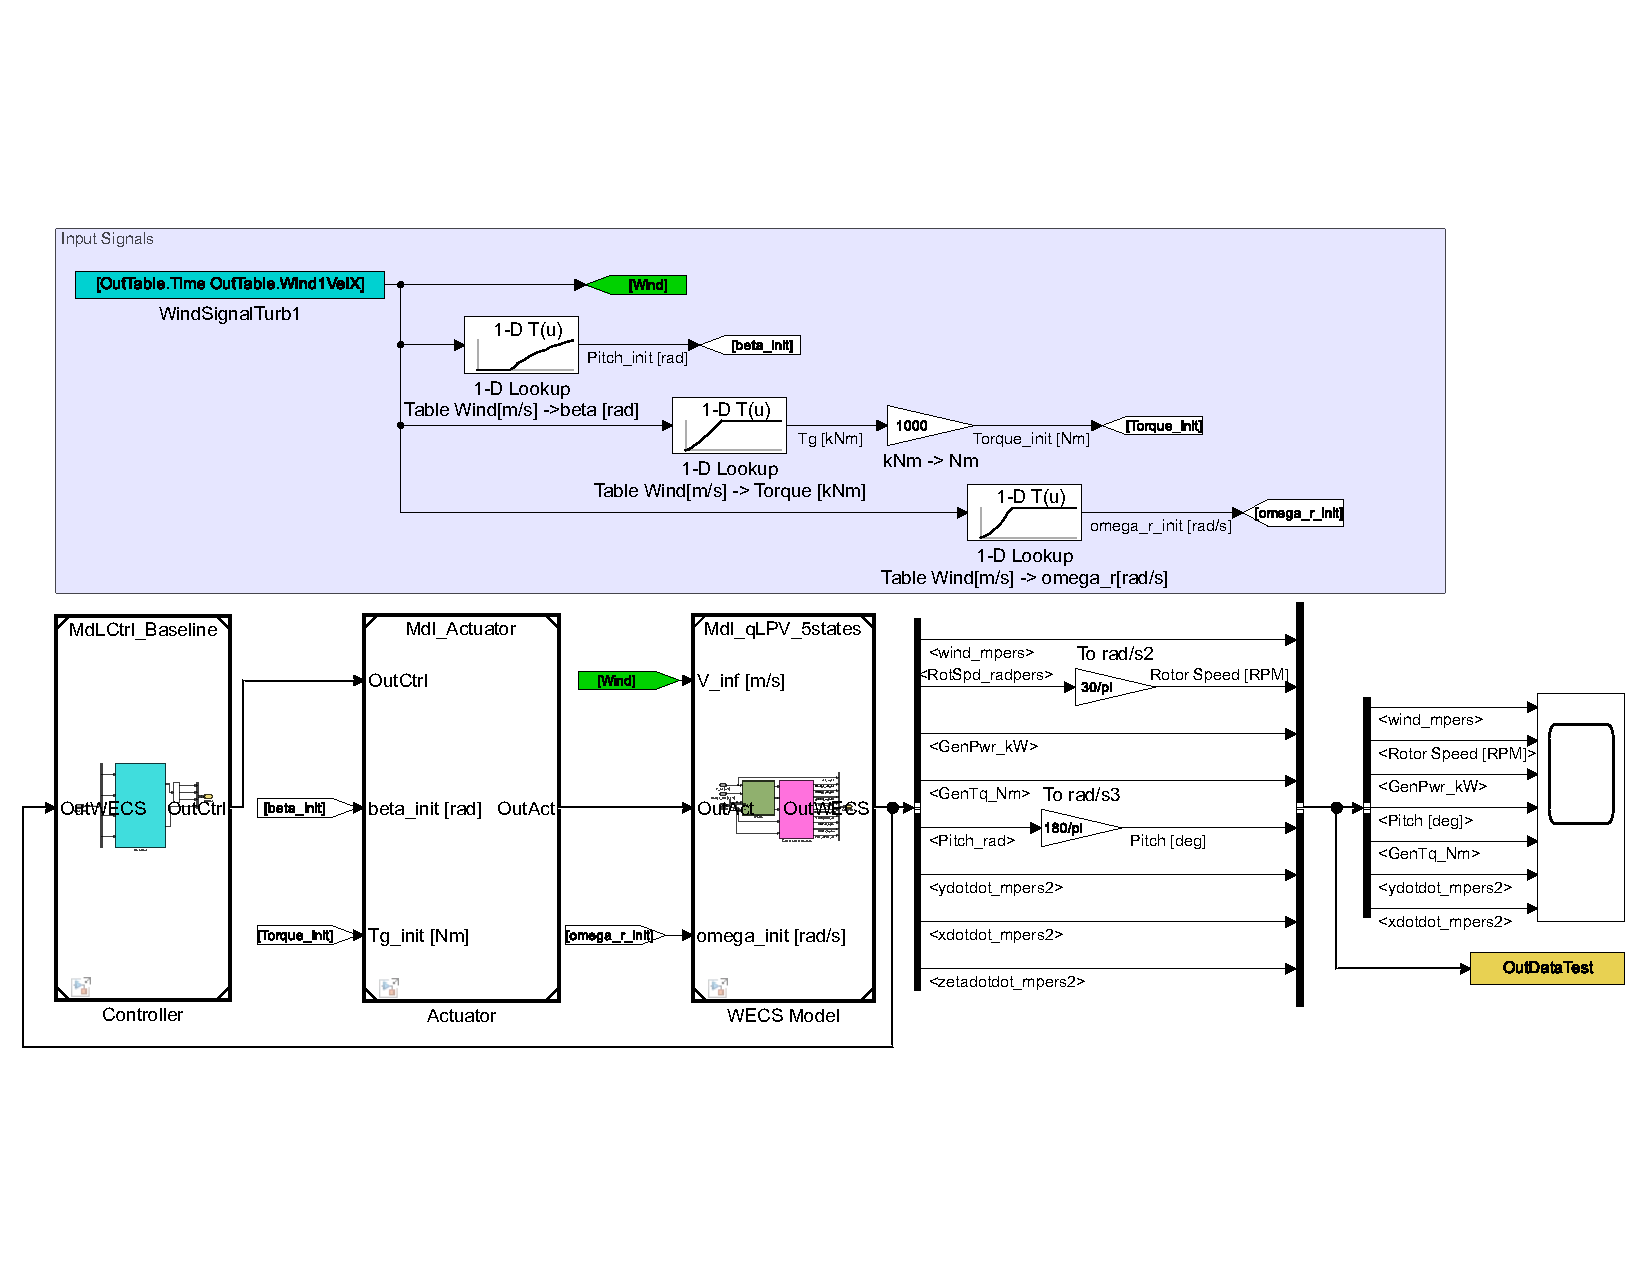
\includegraphics[width=0.9\textwidth, trim={0.2cm 3cm 0.2cm 3.5cm}, clip]{figures/figures_Simulink/test_SimulinkMdl1_Baseline.pdf}
        \caption[Simulink model for closed-loop verification including controller, actuator, and WECS model.]{Simulink model for closed-loop verification including controller, actuator, and WECS model. The wind is created with the FASTTool and used for the initialization of the generator torque, the blade pitch and the rotor speed.}
        \label{fig:baseline_simulink}
    \end{figure}
    
    \begin{figure}[H]
        \centering
        \subfloat[5th-order model with rotor speed and tower displacement states, adapted from \cite{mulders2020preventing}.\label{fig:tudelft_ol_wecs}]{%
            \includegraphics[width=0.9\textwidth, trim={0.2cm 0.5cm 0.2cm 1.cm}, clip]{figures/figures_Simulink/Mdl_TuDelftOL_WECS.pdf}
        }\\[1em]
        \subfloat[9th-order model with rotor and generator speed as well as tower and blade displacement states, adapted from \cite{Bianchi2007}.\label{fig:bianchi_ol_wecs}]{%
            \includegraphics[width=0.9\textwidth, trim={0.1cm 2cm 0.2cm 2.8cm}, clip]{figures/figures_Simulink/Mdl_BianchiOL_WECS.pdf}
        }
        \caption[Simulink implementations of the two qLPV WECS models.]{Simulink implementations of the two qLPV WECS models. Both models use 2D lookup tables for the torque and thrust coefficients $c_Q$ and $c_T$, and have as inputs wind speed $V_\infty$, blade pitch angle $\beta_0$, and generator torque $T_g$.}
        \label{fig:ol_wecs_models}
    \end{figure}
    The Simulink model used for testing includes the controller, the actuator, and the Wind Energy Conversion System (WECS) model through model references. Hence, the controller block can easily be set to contain either the PI baseline controller or one of the qLMPC versions. Similarly, the WECS model block can either contain one of the qLPV model implementations presented in Figure~\ref{fig:ol_wecs_models} or a FAST implementation integrated via an S-function. Note that in this section, the wind turbine model included in the Simulink implementation for closed-loop testing is either the 5th-order model from Figure~\ref{fig:ol_wecs_models}(a) or the 9th-order model displayed in Figure~\ref{fig:ol_wecs_models}(b). The FAST reference signals are taken from the same simulation run that generates the wind vector used to excite the qLPV models.
    
    The baseline controller relies solely on generator speed feedback \(\omega_g\) and operates based on different control strategies across the turbine's operational regions. In Regions~I~1/2 and~II, the generator torque is determined using a \(k\omega^2\) control law, derived from a tabulated function of \(\omega_g\), maximizing power yield below rated wind speed. In Region~III, a gain-scheduled PI controller modulates the collective blade pitch angle \(\beta_0\) to regulate power output. The proportional and integral gains, \(K_P(\omega_g)\) and \(K_I(\omega_g)\), are dynamically scheduled to track and maintain the rated rotor speed.
    
    To prevent excitation of structural resonances, the FASTTool controller includes filters on the generator speed signal, such as a low-pass filter and two notch filters. The pitch control signal \(\beta_{0,\text{ref}}\) is determined based on the filtered generator speed \(\omega_{g,\text{filt}}\), ensuring stable power regulation above rated wind speed while mitigating structural loads. The controller allows for user selection between constant and gain-scheduled PI coefficients, with the latter used as the default setting, as detailed in \cite{mulders2020wind}.
    
    To generate the wind for the test cases, FASTTool is used. This environment is a MATLAB-based graphical user interface designed for configuring simulations and tuning controller parameters. It uses the Fortran-based FAST NREL 5MW wind turbine model implementation and integrates it into Simulink as an S-function. The baseline power controller is implemented using Simulink blocks and MATLAB functions. This controller is used to control both wind turbine models introduced above, as well as the Simulink S-function implementation of the FAST model. In the MIMO controller architecture presented in the next chapter, both the pitch and generator torque controllers of the baseline controller are replaced by the qLMPC scheme. For model verification purposes, however, the original Simulink implementation of the baseline controller is retained. 
    
    To verify the models, two simulations are performed using the original setup, including the baseline controller and the FAST NREL 5MW model implemented as an S-function. The first simulation consists of a wind-speed sweep from 4\,m/s to 25\,m/s in increments of 1\,m/s. Each wind-speed level is maintained for 100\,s to ensure that steady-state conditions are reached. This test is used to verify that the models converge to the same steady-state operating points and to compare their transient responses to wind-speed changes. The second simulation uses a turbulent wind field with a mean wind speed of 18\,m/s and turbulence class B, corresponding to a turbulence intensity of 14\%. This simulation is used to investigate the qLPV models' responses to turbulent wind conditions. The first simulation is run for 2200\,s and the second for 660\,s. Both simulations are executed with a sampling time of 8\,ms, and the generated wind data are stored. Using these recorded wind speed time series, the simulations are repeated with the FAST NREL 5MW S-function replaced by the Simulink implementations of the qLPV models.
    
    %\newpage
    \subsection{Results}\label{subsec:ResultsqLPVModel}
    This section presents the open-loop frequency domain and closed-loop time domain verification of the two qLPV models. All wind fields and test cases are available in the Git repository~\cite{GitRepoCodeqLMPC}, which also includes the code to reproduce all qLPV models presented here. 
    \subsubsection*{Results of the Open-Loop Frequency Domain Verification}
    Figures~\ref{fig:Bode4} and~\ref{fig:Bode12} depict the magnitude response of four linear models: two models at the boundary wind speeds of 4\,m/s and 25\,m/s, and two models near the rated wind speed of 11.4\,m/s (specifically at 11\,m/s and 12\,m/s). Corresponding linearized FAST models serve as the reference.
    \begin{figure} [htp]\centering
        
        \subfloat[Wind speed $V_{\infty} = 4$\,m/s]{\includegraphics[width=0.75\textwidth]{Figures_ADi/BodeV4.eps}}\\
        \subfloat[Wind speed $V_{\infty} = 11$\,m/s]{\includegraphics[width=0.75\textwidth]{Figures_ADi/BodeV11.eps}}
        \caption[Open-loop verification: Frequency response magnitude of linearized FAST and qLPV models for below-rated wind speeds.]{Open-loop verification: Frequency response magnitudes of the linearized FAST and qLPV models for below-rated wind speeds. The 5th-order model Mdl1~(\mlBlackDashed, rotor and tower dynamics) and the 9th-order model Mdl2~(\mlBlue, rotor, generator, tower, and blade dynamics), together with the 30th-order FAST reference implementation~(\mlOrange), are compared over the frequency range of 0.01\,Hz to 2\,Hz.} %
        \label{fig:Bode4}
    \end{figure}
    \begin{figure} [htp]\centering
        \subfloat[Wind speed $V_{\infty} = 12$\,m/s]{\includegraphics[width=0.75\textwidth]{Figures_ADi/BodeV12.eps}}\\ 
        \subfloat[Wind speed $V_{\infty} = 25$\,m/s]{\includegraphics[width=0.75\textwidth]{Figures_ADi/BodeV25.eps}}
        \caption[Open-loop verification: Frequency response magnitude of linearized FAST and qLPV models for above-rated wind speeds.]{Open-loop verification: Frequency response magnitudes of the linearized FAST and qLPV models for above-rated wind speeds. The 5th-order model Mdl1~(\mlBlackDashed, rotor and tower dynamics) and the 9th-order model Mdl2~(\mlBlue, rotor, generator, tower, and blade dynamics), together with the 30th-order FAST reference implementation~(\mlOrange), are compared over the frequency range of 0.01\,Hz to 2\,Hz.} 
        \label{fig:Bode12}
    \end{figure}
    
    For all models, the frequency range from 0.01\,Hz to 2\,Hz is evaluated. Note that typically only the range up to 1\,Hz is considered in the literature, e.g., \cite{schlipf2013nonlinear} or \cite{pamososuryo2022individual}, as this interval contains the dominant first tower and blade modes. The magnitude response of the first (5th-order) model, Mdl1, is shown in black, the second (9th-order) model, Mdl2, in blue, and the linearized FAST reference in red. The latter's 30 states include all states of the derived qLPV models alongside additional structural degrees of freedom. The plots visualize the transfer functions from the control inputs (generator torque and blade pitch) and the disturbance (wind speed) to the rotor speed and tower fore-aft and side-to-side acceleration.
    
    The comparison shows a good fit to the linearized FAST reference for both models from 0.01\,Hz up to the first tower natural frequency at approximately 0.32\,Hz, except for the side-to-side response to blade pitch and wind speed discussed below. The second model also demonstrates a reasonable fit at the first blade natural frequency around 0.7\,Hz. However, the frequency response above 1\,Hz deviates from the FAST model. This deviation is due to higher-order dynamics present in the 30th-order linearized FAST model that are not captured in these simpler models. Thus, while the overall fit is reasonable, some discrepancy with the higher-order linearized FAST model is inevitable across different channels.
    
    In the first column, the frequency response from the generator torque input is shown. From 0.01\,Hz up to approximately 0.7\,Hz, both reduced-order models follow the FAST reference closely. This is true for all four wind speeds and all three depicted outputs, i.e., the rotor speed and the tower fore-aft and side-to-side acceleration. Above 0.7\,Hz, the fit deteriorates, especially around 1\,Hz, where the FAST reference shows an additional resonance, likely caused by modes such as the first edgewise blade modes at approximately 1.1\,Hz, which are not captured by either reduced-order model.
    
    The second column shows the response to the blade pitch input. Blade pitch is not used for control below rated wind speed, as in Figure~\ref{fig:Bode4}, and remains near a fixed angle. The pitch-to-output response therefore reflects the underlying open-loop aeroelastic dynamics, in which blade structural modes play a dominant role. As a result, differences between the reduced-order models become more visible in this channel. Looking at the response of the rotor speed to the blade pitch, the agreement between the FAST reference and Mdl2 is considerably better than with Mdl1. The advantage of the model with blade dynamics is also clear in the tower fore-aft acceleration response, where it reproduces the blade frequency peak around 0.7\,Hz, especially at 4\,m/s in Figure~\ref{fig:Bode4}(a). At higher wind speeds, see Figure~\ref{fig:Bode12}, this peak is less pronounced, and differences among models diminish. Still, Mdl2, which includes blade dynamics, consistently provides a slightly better overall fit across the full frequency range for the responses of the rotor speed and tower fore-aft acceleration. In the tower side-to-side acceleration response of the lower wind speeds shown in Figure~\ref{fig:Bode4}, an offset can be seen between the FAST reference and both models over the whole frequency range, with the magnitude of both models being consistently below the reference magnitude. In both models, blade pitch excites the side-to-side motion only through the rotor torque contribution $(1-c_{M_x})\,T_r$ to the torsional nacelle moment, i.e., only about 12\% of the rotor torque variations, whereas the FAST reference includes additional in-plane load paths not represented in the reduced-order models. For the higher wind speeds in Figure~\ref{fig:Bode12}, the fit improves, with the magnitude fitting well for frequencies between 0.07\,Hz and 0.2\,Hz in Figure~\ref{fig:Bode12}(b). The magnitude of the peak at approximately 0.32\,Hz is still underpredicted by Mdl1 and Mdl2.
    
    The third column depicts the response to variations in wind speed. In the rotor speed response, a notch appears in the FAST reference at approximately 0.3\,Hz, the frequency of the first tower mode, across all wind speeds. Both qLPV models reproduce this notch, albeit shallower. At higher frequencies, however, Mdl1 continues along a smooth, monotonic decline, while Mdl2 dips more sharply at 0.7\,Hz before recovering to follow the slope of Mdl1. FAST does not dip at 0.7\,Hz, but at 0.8\,Hz for the two lower and around 1\,Hz for the higher wind speeds. However, the amplitude of Mdl2 is still closer to this reference than that of Mdl1. In the tower fore-aft acceleration response, both models again match FAST well through the tower peak at roughly 0.3\,Hz. Past the peak, Mdl2 continues to track the FAST reference's small increase at 0.7\,Hz, whereas Mdl1 diverges gradually as its response flattens. In both of these channels, Mdl2 therefore clearly outperforms Mdl1 at higher frequencies. In the tower side-to-side response, on the other hand, Mdl1 and Mdl2 remain close to one another throughout the frequency range, but deviate from the FAST reference at low frequencies. At 4\,m/s in Figure~\ref{fig:Bode4}(a), both models lie below the FAST reference, with the gap closing towards 0.2\,Hz. At 11\,m/s and above, the FAST reference shows a notch between approximately 0.02\,Hz and 0.05\,Hz, shifting to higher frequencies with increasing wind speed. At frequencies below this notch, the FAST reference lies above both models. At frequencies above the notch, the reference's magnitude is below that of both models. All three responses converge between approximately 0.1\,Hz and 0.2\,Hz. As in the pitch channel in column two, the deviation is attributed to the wind exciting the side-to-side motion in both models only through the rotor torque contribution $(1-c_{M_x})\,T_r$, whereas additional in-plane load paths in the FAST reference interfere with this contribution and cause the notch. At the tower peak at roughly 0.3\,Hz, the magnitude is underpredicted by both models for all wind speeds. Above this peak, the simpler Mdl1 follows the FAST reference relatively well, while Mdl2 exhibits a dip near 0.8\,Hz that is absent from the FAST reference, and the FAST reference shows additional resonances at approximately 1.1\,Hz and 1.5\,Hz. Since the side-to-side dynamics are driven by the rotor speed, the fore-aft tower velocity and the inputs, but do not feed back into the rotor speed or fore-aft dynamics in either model, the weaker open-loop fit in this channel does not affect the remaining responses. To verify that the reduced-order models accurately capture the dynamics within the frequency range relevant for control, a time-domain comparison with the FAST reference is also carried out in closed-loop operation.
    
    
    \subsubsection*{Results of the Closed-Loop Time Domain Verification}    
    For the verification in closed loop, two representative wind scenarios are considered: a stepped wind speed sweep from 4\,m/s to 25\,m/s, and a turbulent wind input with a mean speed of 18\,m/s.
    %
    Figure~\ref{fig:TimeCmpMdlSweep}(a) shows the results for the stepped wind sweep across all three closed-loop models. The wind increases in steps of 1\,m/s every 100\,s. The first 60\,s of the simulation, which contain initialization artifacts, are omitted. As a result, 40\,s of excitation are shown for 4\,m/s, and 100\,s for all other wind speeds. Figure~\ref{fig:TimeCmpMdlSweep}(b) presents the signals between 600\,s and 1000\,s of simulation time, corresponding to wind speeds between 10\,m/s and 13\,m/s. As before, the signals of the 5th-order model are plotted in black (dashed), the 9th-order model in blue, and the FAST model in red.
    %
    \begin{figure}[h]
        \centering
        \subfloat[Stepped wind sweep from 4\,m/s to 25\,m/s]{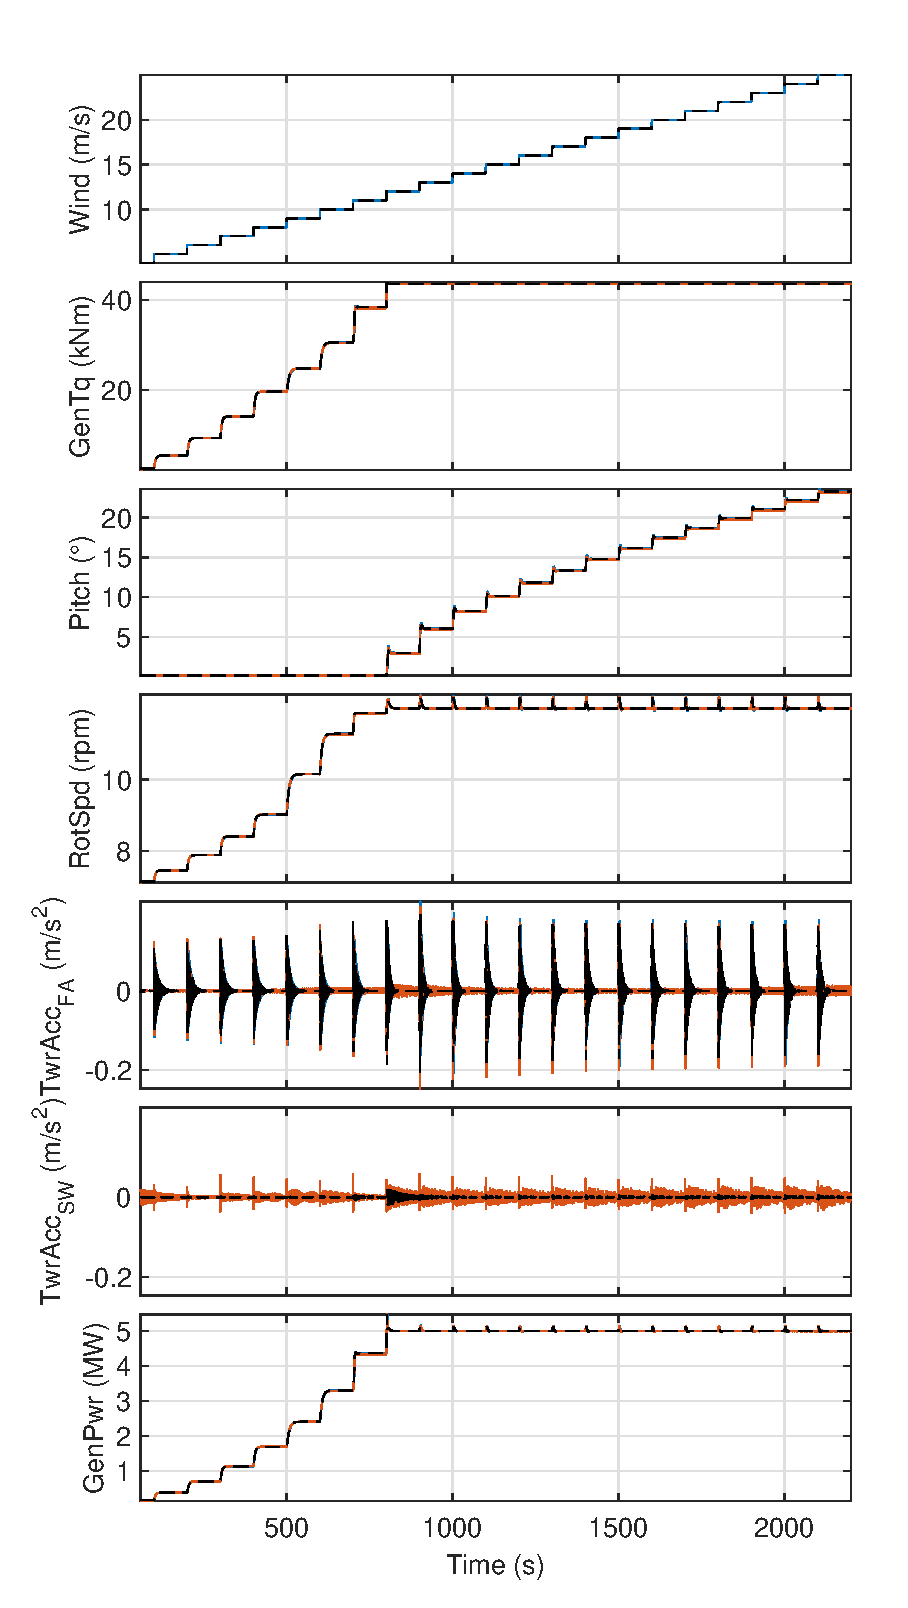
\includegraphics[width=0.485\textwidth, trim={0cm 0cm 0cm 1cm},clip]{figures/Figures_ADi/cmpTimeDomain_AllStep.eps}}\hspace{0.01\textwidth}
        \subfloat[Zoom on wind speed range 10\,m/s to 13\,m/s]{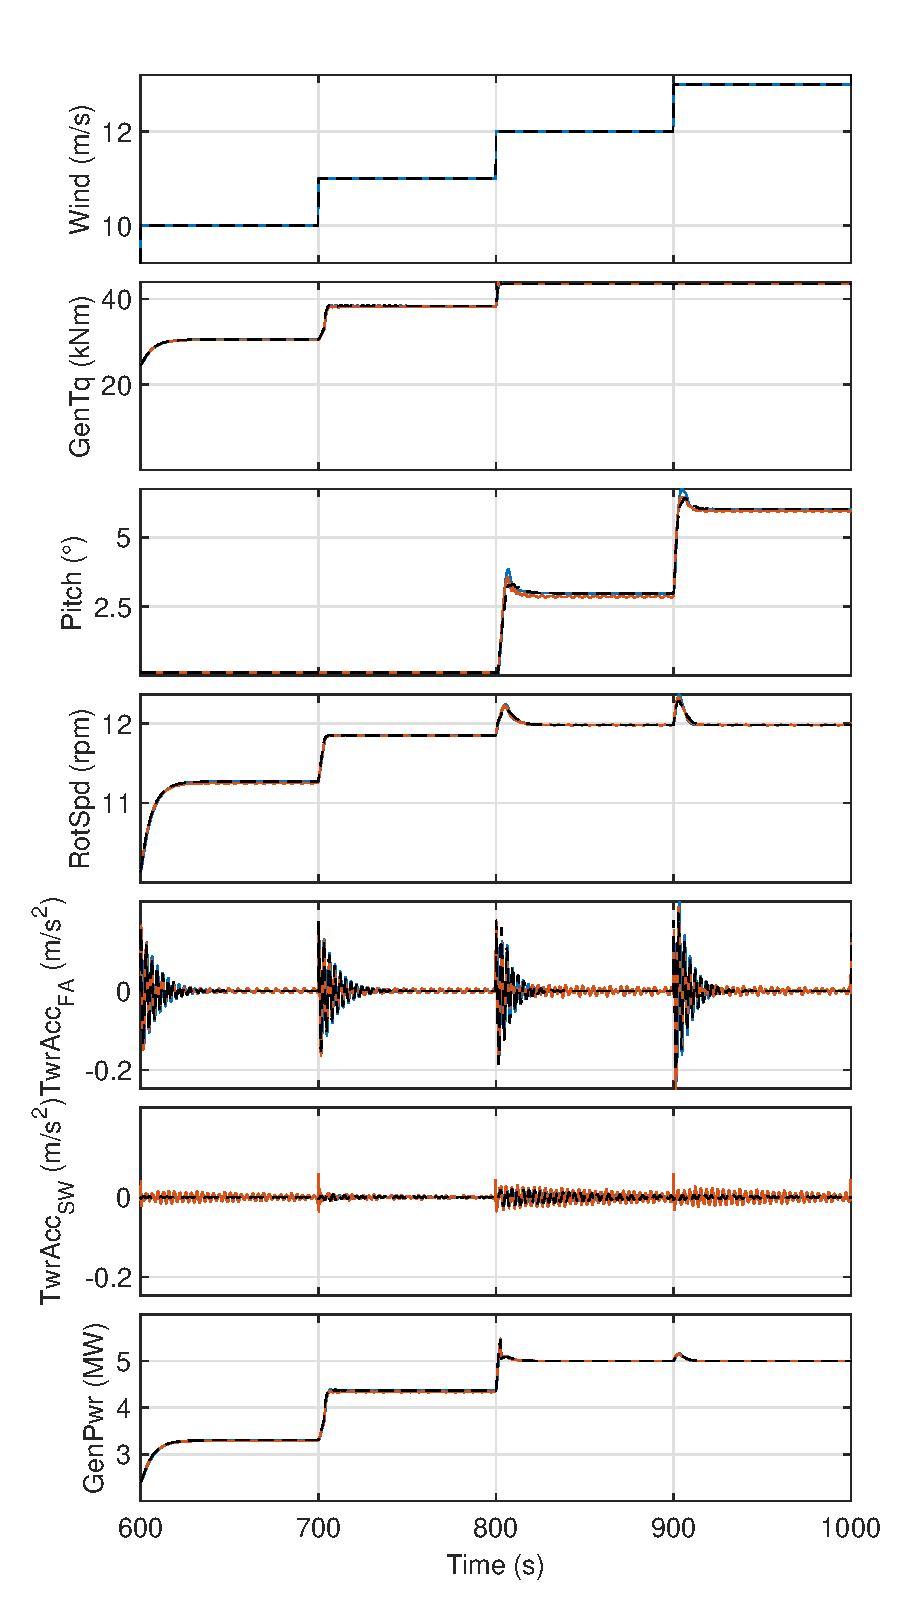
\includegraphics[width=0.485\textwidth, trim={0cm 0cm 0cm 1cm},clip]{figures/Figures_ADi/cmpTimeDomain_AllZoomStep.eps}}
        \caption[Closed-loop verification: FAST and qLPV models with PI baseline 
        controller, stepped wind sweep 4\,m/s to 25\,m/s.]%
        {Closed-loop verification: FAST and qLPV models simulated in closed loop with the PI baseline controller with a stepped wind sweep from 4\,m/s to 25\,m/s. 
            Mdl1~(\mlBlackDashed, rotor and tower dynamics),  Mdl2~(\mlBlue, rotor, generator, tower, and blade dynamics), and FAST reference~(\mlOrange). Displayed signals: wind, control inputs, 
            rotor speed, tower accelerations, and power.}
        \label{fig:TimeCmpMdlSweep}
    \end{figure}
    %
    The first subplot shows the wind input applied to the turbine, which is identical for all simulations. The second and third subplots display the two control inputs: generator torque and collective blade pitch. The fourth subplot shows the rotor speed, followed by the fifth and sixth subplots showing the tower fore-aft and side-to-side accelerations, respectively. The final subplot depicts the resulting electrical power output. There is a very good fit between FAST and both models for the stepped wind sweep test case, in the transient dynamics as well as in the steady-state gain. Small deviations remain, e.g., a slight steady-state pitch offset of Mdl1 above rated wind speed and a slightly larger pitch overshoot of Mdl2 after the step at 800\,s, see Figure~\ref{fig:TimeCmpMdlSweep}(b). The good fit in steady state corresponds to the resemblance between FAST and both models for the rotor speed and the tower fore-aft acceleration for lower frequencies. As there is little difference both in the generator torque as well as in the rotor speed, there is also a good fit in the power output. There is also a good fit in the amplitude of the fore-aft tower acceleration for all wind speeds. In the tower side-to-side acceleration, both models reproduce the oscillations above rated wind speed with a similar amplitude, but do not capture the short peaks at the wind steps and the continuous low-level oscillation present in the FAST reference. However, the amplitudes of this signal are comparatively small and its influence on the overall dynamics is nearly negligible.
    %
    Figure~\ref{fig:TimeCmpMdlNTM} shows the second test case: a turbulent wind profile with a mean speed of 18\,m/s and turbulence class~B of the International Electrotechnical Commission (IEC). This test case reveals a limitation of the qLPV models, which represent wind as a scalar value acting uniformly on the rotor, rather than as a spatially distributed field.
    \begin{figure}[htbp]
        \centering
        \subfloat[No filter]{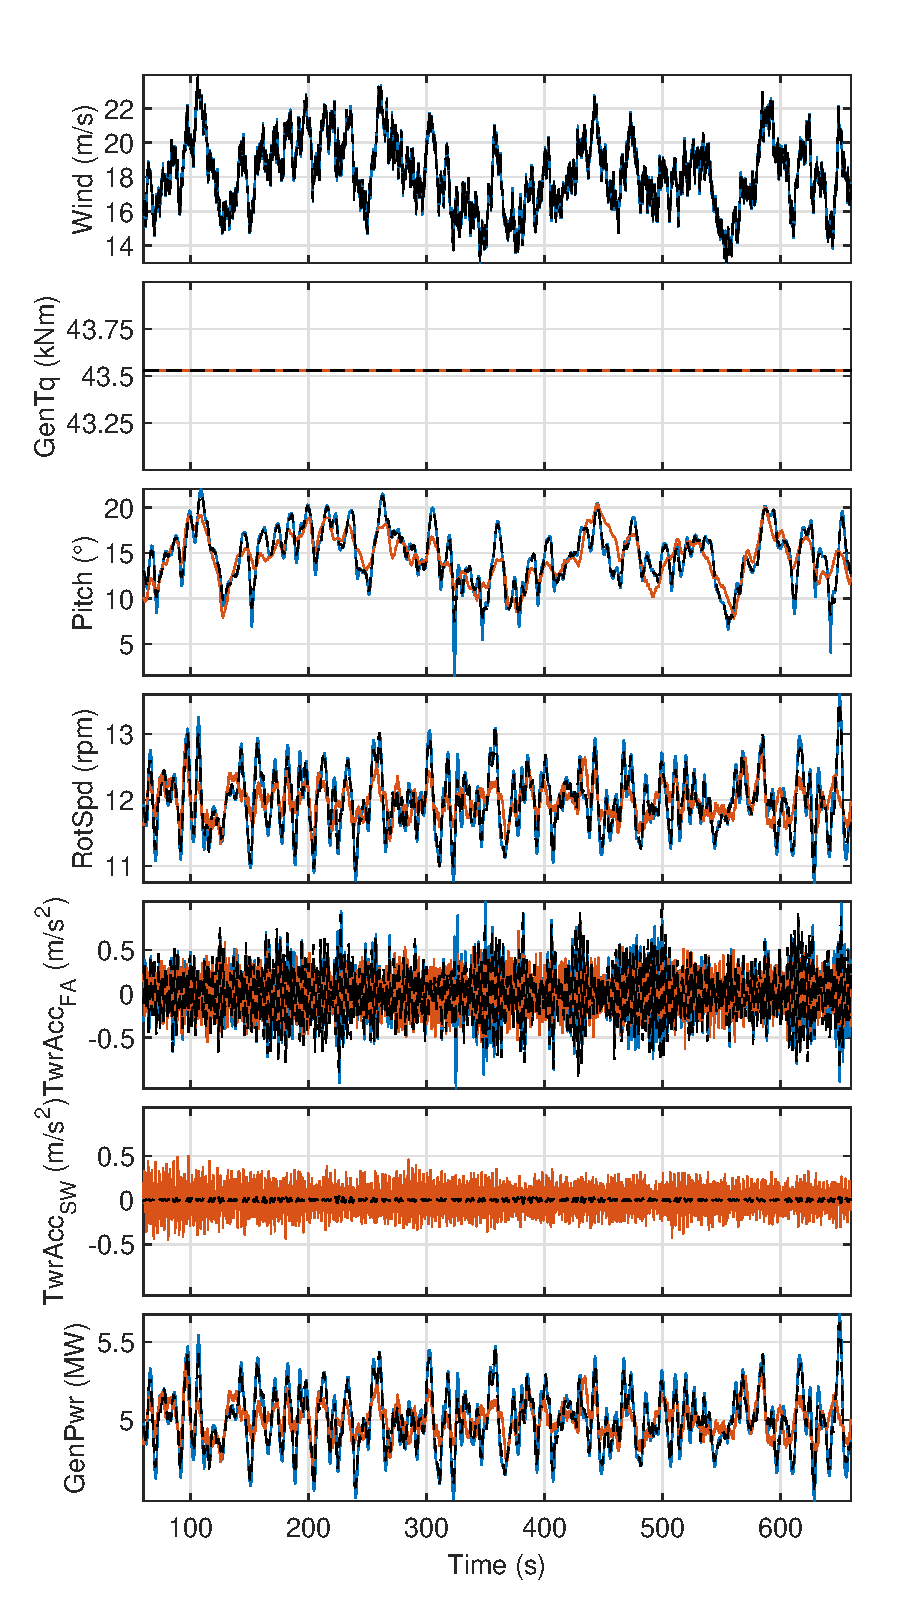
\includegraphics[width=0.485\textwidth, trim={0cm 0cm 0cm 1.cm},clip]{figures/Figures_ADi/cmpTimeDomain_AllNTW18.eps}}\hspace{0.01\textwidth}
        \subfloat[Filter with $k_\tau = 0.75$ and  $k_T = 0.25$ ]
        {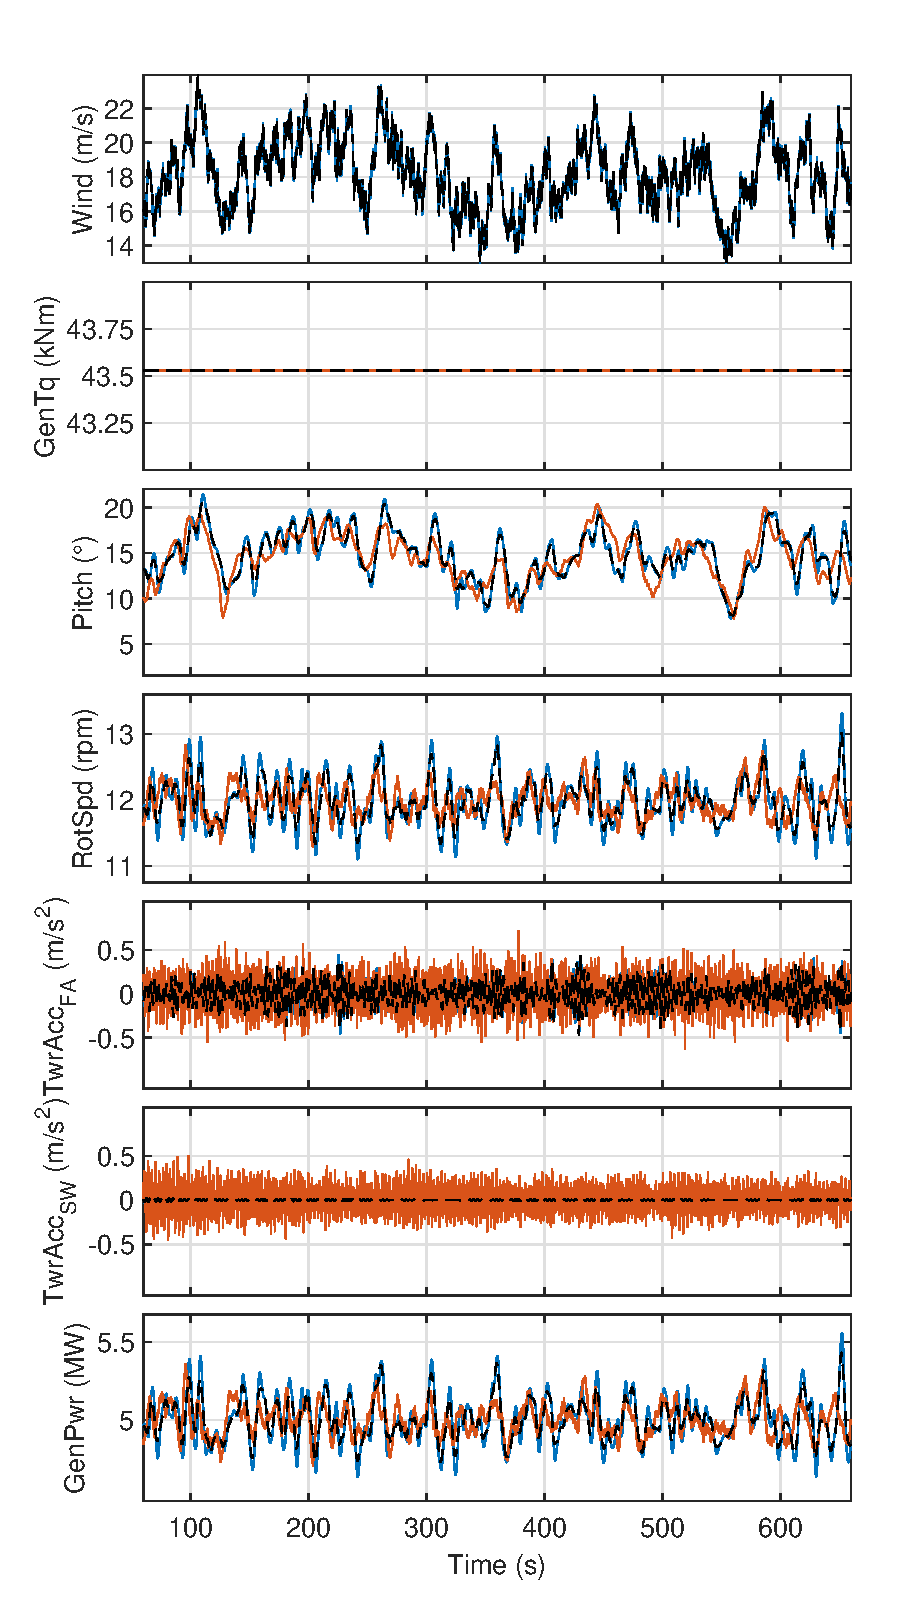
\includegraphics[width=0.485\textwidth,trim={0cm 0cm 0cm 1.cm},clip]{figures/Figures_ADi/cmpTimeDomain_AllNTW18_kVe0dot25_kVeTau0dot75.eps}}
        \caption[Closed-loop model comparison: FAST and qLPV models with PI baseline 
        controller, under turbulent wind with and without filter on freestream wind.]{Closed-loop model comparison: FAST and qLPV models with PI baseline controller, under turbulent wind (18\,m/s mean, turbulence 
            class B), with and without filter on freestream wind. Mdl1 (\mlBlackDashed, rotor and tower dynamics),  Mdl2~(\mlBlue, rotor, generator, tower, and blade dynamics), and FAST reference~(\mlOrange). Displayed signals: wind, control inputs, rotor speed, tower 
            accelerations, and power.}
        \label{fig:TimeCmpMdlNTM}
    \end{figure}
    In a real turbine, the large rotor disk acts as a natural low-pass spatial filter, averaging out high-frequency point gusts across its swept area. Because single-point freestream wind data cannot represent this spatial coherence, feeding an unfiltered point velocity into the low-order lookup tables causes the model to respond excessively to high-frequency variations. At the same time, the structural tower dynamics are driven by the aerodynamic thrust and blade-passage effects, which require a faster excitation spectrum. To address this discrepancy, the freestream wind speed is filtered before entering the aerodynamic lookup tables, with separate filters for the torque and thrust channels, yielding the filtered wind speeds $V_{\text{filt},\tau}$ and $V_{\text{filt},T}$. The underlying idea is that a gust is averaged over the rotor while the wind travels across it. Hence, the time constant of each filter is set to the time the wind needs to travel a distance $k_i R_r$, i.e., a fraction $k_i$ of the rotor radius, which makes the filter faster at high wind speeds. Before filtering, the freestream wind speed is projected onto the rotor axis by the factor $\cos(5^\circ)$ to account for the shaft tilt of the NREL 5MW turbine. For a constant wind speed, the resulting first-order low-pass filters can be expressed by the transfer functions
    \begin{align*}
        \frac{V_{\text{filt},i}(s)}{V_\infty(s)} = \frac{\cos(5^\circ)}{T_i s + 1}, \qquad T_i = \frac{k_i R_r}{\cos(5^\circ)\,V_\infty}, \qquad i \in \{\tau, T\},
    \end{align*}
    where $s$ denotes the Laplace variable; in the simulation, the time constant $T_i$ is updated with the current wind speed $V_\infty(t)$. The scaling factors $k_\tau = 0.75$ and $k_T = 0.25$ are chosen such that the torque channel is smoothed more strongly, while the thrust channel preserves the faster excitation relevant for the tower dynamics. The filters are implemented in discrete time with the sampling time $\Delta t$ as
    \begin{align*}
        V_{\text{filt},i}(k) = V_{\text{filt},i}(k-1) + \alpha_i(k)\left(V_{\text{in}}(k) - V_{\text{filt},i}(k-1)\right), \qquad \alpha_i(k) = 1 - e^{-\frac{\Delta t\,V_{\text{in}}(k)}{k_i R_r}},
    \end{align*}
    with the projected input $V_{\text{in}}(k) = \cos(5^\circ)\,V_\infty(k)$. For the wind steps of the first test case, the filter can be bypassed by setting $\alpha_i = 1$. By default, the Simulink implementations of Mdl1 and Mdl2 include neither the wind filter nor the rotor tilt of 5\textdegree{}. Simulations showed that applying the projection $\cos(5^\circ)$ consistently to the plant and to the wind of the qLMPC changes the standard deviations and their ratios in turbulent wind by less than 1\%. The projection is nevertheless included in the rotor-effective wind filter, since the filter converts the hub height wind into the wind acting on the rotor and is thus the natural place for this geometric correction, which keeps the filtered model as close to the physics as possible. The precone of 2.5\textdegree{}, in contrast, is a property of the rotor geometry rather than of the wind direction and is therefore not included in the projection.
    
    %
    As shown in Figure~\ref{fig:TimeCmpMdlNTM}(a), without filtering the models exhibit pronounced high-frequency oscillations and overshoot in blade pitch, rotor speed, and generator power, as well as an overestimated tower fore-aft acceleration. For Mdl2, the rotor speed overshoot even causes a short drop in generator torque and power at approximately 325\,s. With the filter active in Figure~\ref{fig:TimeCmpMdlNTM}(b), the blade pitch, the rotor speed fluctuations, and the power follow the FAST reference more closely, but are still slightly larger and the tower fore-aft acceleration amplitude is underestimated by both models. The tower side-to-side acceleration is not reproduced very accurately by either model in this test case, as it is mainly excited by asymmetric rotor loads resulting from the spatially distributed wind field, which cannot be represented by a scalar wind input. Unless stated otherwise, the qLMPC designs of Chapter~\ref{sec:Application to Wind Turbine Control4} use the unfiltered freestream wind speed $V_\infty$; the filters are additionally applied for the evaluation on the filtered plant and in the qLMPC designs for FAST, where the controller is scheduled with $V_{\text{filt},\tau}$.
    %
    It should also be noted that some minor discrepancies remain in Figure~\ref{fig:TimeCmpMdlSweep}, such as small oscillations in the tower movement due to the additional degrees of freedom of FAST. However, the reduced-order models capture the dominant system dynamics with sufficient accuracy for control design. Both Mdl1, without blade dynamics, and Mdl2, with an additional out-of-plane blade degree of freedom, show good agreement with the FAST reference during the stepped wind sweep.  But Mdl2 shows a slightly better alignment in the blade pitch to rotor speed channel and additionally provides the out-of-plane blade motion. Therefore, Mdl2 is selected as the plant model for the qLMPC design on the qLPV model, and its states are the basis of the qLMPC prediction models in Chapter~\ref{sec:Application to Wind Turbine Control4}.
    %Mdl2 captures a broader range of dynamics, most notably in the blade pitch to rotor speed channel, where it shows better alignment with FAST due to the inclusion of blade dynamics.
    \chapter{Wind Turbine Control}  \label{sec:Application to Wind Turbine Control4} 
Modern megawatt wind turbines are both speed-controlled and pitch-controlled \cite{pao2011control,mulders2018delft, elkodama2023control}. Controllers and their parameters are often fine-tuned to
fit not only a specific wind turbine type but also individual turbines, taking into account factors
such as manufacturing and installation variations, including rotor blade weight imbalances and
aging processes \cite{en14238083}. These conventional feedback control designs, typically relying
solely on generator speed as input and controlling the blade pitch angles collectively, are
well-engineered and technologically mature. However, further reduction of the cost of energy
production can be achieved by introducing additional control inputs or sensors. Moreover, using a
predictive scheme like qLMPC allows leveraging wind measurements or estimates and incorporating
this information over a prediction horizon. It also accounts for how the system states, e.g., the
rotor and generator speed, are expected to react to the wind trajectory and future control inputs
within that horizon. This chapter investigates control strategies that leverage such improvements:
a qLMPC design, which incorporates wind information, and PI Individual Pitch Control
(IPC), the latter both as a standalone method and in combination with Trailing Edge Flap Control
(TEFC), aimed at reducing mechanical loads. These control approaches are evaluated in terms of
power reference tracking, actuator activity, and mechanical loads.
%
In Section~\ref{sec:quasiLPVMPCDesign}, the design of a velocity-based qLMPC controller based on
the first-principles model of Chapter~\ref{sec:WindTurbineqLPVModels} is presented. Whereas qLMPC
has so far been applied to wind turbines as a SISO scheme \cite{mulders2020preventing, pamososuryo2022individual,
    fonseca2024windTurbineSideSide}, the design presented here actuates generator torque and
collective pitch simultaneously as a MIMO scheme, covering the entire operating range. It is
reformulated as a QP and solved via a linear complementarity formulation with Lemke's algorithm
\cite{cisneros2020velocity}, yielding mean solver times below 2\,ms at a controller sampling time
of 8\,ms and thus real-time capability.
%
Section~\ref{section:Individal Pitch PI Control} introduces IPC, explaining the multiblade
coordinate transformation and comparing IPC simulation results to those from baseline Collective
Pitch Control (CPC). The simulation environment is also used to tune the IPC gains by a Nelder-Mead simplex optimization of the blade root Damage Equivalent Load (DEL), followed by
a constrained optimization that limits the tower base DEL.
%
Section~\ref{sec:CombinedIPC-TrailingEdgeFlapControl} describes the combination of IPC and TEFC, in the following called Active Aerodynamic Load Control (AALC), including the necessary model extensions and the achieved load reductions on the blades and tower. Whereas earlier studies combining the two actuation principles report results for single mean wind
speeds \cite{wilson2009combined, henriksen2013model, he2018combined}, the controller presented
here is demonstrated across Regions II and III, using one training dataset and two independent
verification datasets.
%
Section~\ref{subsec:ComparisonWindTurbineControlDesigns} compares qLMPC, IPC, and AALC, discussing the potential of the different schemes and showing the trade-offs between DEL reduction and actuator activity relative to the PI CPC
baseline. 
The results for the qLMPC applied to the qLPV model presented in Chapter~\ref{sec:WindTurbineqLPVModels} have been published in \cite{dittmer2021velocity}. They are extended here with results of the qLMPC applied to FAST and with modifications to the algorithm that improve its performance when applied to FAST. The AALC strategy has been published in \cite{dittmer2024combined}. It is extended here by a detailed discussion of the optimization of an IPC algorithm without Trailing Edge Flaps (TEFs), fine-tuned in the simulation environment of the AALC. The AALC parameters are re-optimized leveraging the IPC parameters optimized before.

%The results for the qLMPC controller have been published in \cite{dittmer2021velocity}, and the AALC control strategy in \cite{dittmer2024combined}.

\section{qLMPC Design and Application}\label{sec:quasiLPVMPCDesign} 
Wind turbine controller design in the above-rated region focuses on smooth power control and in the below-rated region on power optimization, as described in \cite{Bianchi2007}. The proposed MIMO qLMPC uses two control inputs, the collective pitch command $\beta_{0,\text{ref}}$ and the generator torque reference $T_{g,\text{ref}}$. The baseline controller consists of two SISO controllers, one for generator torque and one for blade pitch control, see Section~\ref{sec:WindTurbineControl}. These can be replaced by a MIMO qLMPC controller, see Figure~\ref{fig:BlockMPC}. 
\begin{figure}[ht]
    \centering
    \includegraphics[width=0.7\textwidth,trim={0 0cm 0cm 0.1cm},clip]{figures/Figures_ADi/turbineCtrlBetaMPC1.pdf}
    \caption[Block diagram of qLMPC replacing the baseline PI controller]{Block diagram of qLMPC replacing the baseline PI controller: the baseline gain-scheduled pitch controller $PI_{GS}(\omega_g)$ and torque controller $k\omega_g^2$ (solid boxes) are replaced by the qLMPC (dashed box). Based on the measured generator speed $\omega_g$ and the estimated wind speed~$\hat{V}_\infty$, it sets the collective pitch reference $\beta_{0,\text{ref}}$ and the generator torque reference $T_{g,\text{ref}}$.}   
    \label{fig:BlockMPC}
\end{figure}
% \caption[Block diagram of the closed-loop wind turbine control structure with qLMPC replacing the baseline PI controller]{Block diagram of the closed-loop wind turbine control structure with qLMPC (dashed box) replacing the baseline PI controller (solid line)}
%
Optimal reference signals $r_\beta$ and $r_{T_g}$ for the two actuator states are calculated from the wind speed $V_\infty$. The cost function penalizes the deviation of the actuator signals $\beta_{0,\text{ref}}$ and  $T_{g,\text{ref}}$ from $r_\beta$ and $r_{T_g}$, the changes of the rotor and generator speed, which in the velocity-based form drive the system to a steady state, and the changes in the control inputs. On the qLPV model, this results in smoother power output and reduced tower movement compared to the baseline. DEL reduction is not an explicit objective of the qLMPC design. However, the six evaluation criteria used to compare all control strategies introduced in Section~\ref{subsection: IPCOptCriteria}, i.e., blade, tower base and tower top DEL, power mean and variance, and actuator activity, are also calculated for this controller to enable a direct comparison with the IPC and AALC designs.

In this work, the velocity-based approach from \cite{cisneros2020velocity}, presented in Section~\ref{sec:qLPVmodels} of this thesis, is applied to a model based on the wind turbine model used for qLPV-based MIMO controller design in \cite{Bianchi2007}. The model in \cite{Bianchi2007} contains three turbine states, the slip angle $\theta_s$ and the rotor and generator speed $\omega_r$ and $\omega_{gr}$, as well as the pitch actuator state $\beta_0$. These four states are a subset of the state vector of the extended model Mdl2$^\prime$ in Equation~\eqref{eq:11} and are sufficient to control the power output. Smoother rotor speed and pitch activity also reduce thrust variations and thus, indirectly, tower and blade movement. Hence, for the sake of simplicity, the decision was made to base the qLMPC scheme on a model close to the one in \cite{Bianchi2007} instead of the extended model Mdl2$^\prime$, as the lower model order reduces the size of the optimization problem and thus the computation time. As control inputs, \cite{Bianchi2007} uses the blade pitch command $\beta_{0,\text{ref}}$ and the zero torque speed $\omega_Z$, which is linearly dependent on the generator torque $T_g$. Three modifications are made to this model:
\begin{enumerate}
    \item The reference generator torque $T_{g,\text{ref}}$ is used as the second control input instead of $\omega_Z$. The reference torque is selected because FAST expects a torque command as input. The optimal trajectory of the reference generator torque $T_{g,\text{ref}}$ over a prediction horizon is calculated based on an optimal reference signal $r_{T_g}$, which is itself calculated from the wind speed.
    \item The generator torque $T_g$, which lags the commanded control signal $T_{g,\text{ref}}$, is used as an additional state to eliminate direct feedthrough, i.e., to avoid a non-zero feedthrough matrix. This fifth state enables the use of the optimization framework for reference tracking and disturbance rejection proposed in \cite{cisneros2020velocity}. Incorporating a filtered control input as an additional state is a common practice, and is, for example, also employed in the MPC algorithm implemented in the Wind Farm Simulator (WFSim) \cite{boersma2018control}. %~\(\bm{D} \)
    \item A desired pitch signal $r_{\beta}$ is used as a reference for the prediction horizon in the MPC optimization to calculate the optimal pitch command $\beta_{0,\text{ref}}$. In \cite{Bianchi2007}, a reference value for the generator speed is tracked. This choice was made to directly optimize the two actuators to avoid handling the large difference in dynamic bandwidth of the actuators and the plant dynamics in the optimization calculation.
\end{enumerate}
%
The resulting state, input and output vectors are given below. As before, different indices are used for the generator speed on the high-speed shaft, denoted $\omega_g$, and the generator speed referred to the low-speed shaft, $\omega_{gr}$. In the state vector, $\omega_{gr}$ is used, as it is in the same reference frame as the rotor speed $\omega_r$:
\begin{equation}\label{eq:xMPCyMPC}
    \begin{aligned}
        \bm{x}_{\text{MPC}} &= [\theta_{s} \quad \omega_r \quad \omega_{gr} \quad T_g \quad \beta_0]^T \in \mathbb{R}^{5 \times 1},\\
        \bm{w}_{\text{Mdl}^\prime} &= [V_{\infty} \quad T_{g,\text{ref}} \quad \beta_{0,\text{ref}}]^T \in \mathbb{R}^{3 \times 1}, \quad
        \bm{y}_{\text{MPC}} = [T_g \quad \beta_0]^T \in \mathbb{R}^{2 \times 1}.
    \end{aligned}
\end{equation}
%
Note that $\bm{y}_{\text{MPC}}$ contains the outputs of the prediction model, i.e., the controlled variables tracked in the cost function, whereas the outputs of the controller are the commanded signals $T_{g,\text{ref}}$ and $\beta_{0,\text{ref}}$ in $\bm{w}_{\text{Mdl}^\prime}$. The nonlinear dynamics of the three turbine states and the two actuator states are:
\begin{align}
    \dot{\theta}_s(t) &= \omega_r(t)-\omega_{gr}(t) \label{eq:NLDyn1},\\
    \dot{\omega}_r(t) &= -\frac{K_{sr}}{J_r}\theta_s(t)-\frac{B_{sr}}{J_r}\omega_r(t)+\frac{B_{sr}}{J_r}\omega_{gr}(t)+\frac{T_r(\omega_r, \beta_0, V_\infty)}{J_r},\\
    \dot{\omega}_{gr}(t) &= \frac{K_{sr}}{J_{gr}}\theta_s(t)+\frac{B_{sr}}{J_{gr}}\omega_r(t)-\frac{B_{sr}}{J_{gr}}\omega_{gr}(t)-\frac{N_g T_g(t)}{J_{gr}} \label{eq:NLDyn3},\\
    \dot{T}_{g}(t) &= -\frac{1}{\kappa}T_{g}(t)+\frac{1}{\kappa}T_{g,\text{ref}}(t),\\
    \dot{\beta}_0(t) &= -\frac{1}{\tau}\beta_0(t)+\frac{1}{\tau}\beta_{0,\text{ref}}(t).\label{eq:NLDyn5}
\end{align}
%
To avoid having to derive a grid of equilibrium points for the different combinations of the state vector, a velocity-based linearization is used.

\subsection{Velocity-Based qLPV Model for Reference Tracking}
The velocity-based linearization method from \cite{cisneros2020velocity}, introduced in Section~\ref{sec:qLPVmodels}, is implemented for the model serving as the basis of the qLMPC design. The nonlinear system dynamics
\[
\dot{\bm{x}}_{\text{MPC}}(t) = \bm{f}_{\text{MPC}}(\bm{x}_{\text{MPC}}, \bm{w}_{\text{Mdl}^\prime}), \quad \bm{y}_{\text{MPC}}(t) = \bm{h}_{\text{MPC}}(\bm{x}_{\text{MPC}})
\]
are described by the relationship between the derivatives of the states, inputs, and outputs:
\begin{align*}
    \ddot{\bm{x}}_{\text{MPC}}(t) &= \nabla_{\bm{x}_{\text{MPC}}} \bm{f}_{\text{MPC}}(\bm{x}_{\text{MPC}}, \bm{w}_{\text{Mdl}^\prime}) \dot{\bm{x}}_{\text{MPC}}(t) + \nabla_{\bm{w}_{\text{Mdl}^\prime}} \bm{f}_{\text{MPC}}(\bm{x}_{\text{MPC}}, \bm{w}_{\text{Mdl}^\prime}) \dot{\bm{w}}_{\text{Mdl}^\prime}(t),\\
    \dot{\bm{y}}_{\text{MPC}}(t) &= \nabla_{\bm{x}_{\text{MPC}}} \bm{h}_{\text{MPC}}(\bm{x}_{\text{MPC}}) \dot{\bm{x}}_{\text{MPC}}(t).
\end{align*}
By considering the derivatives instead of the original states, the need for storing steady-state vectors for input, output, and states at each operating point is eliminated.
As in the actuator-augmented model in Equation~\eqref{eq:11}, the input vector $\bm{w}_{\text{Mdl}^\prime} = [V_{\infty} \;\; T_{g,\text{ref}} \;\; \beta_{0,\text{ref}}]^T$ contains the commanded signals, and the actuator outputs $T_g$ and $\beta_0$ are states.
%
The continuous-time system, input, and output matrices are
\begin{align*}
    \bm{A}_c(\bm{\rho}_\Rho) &= \nabla_{\bm{x}_{\text{MPC}}} \bm{f}_{\text{MPC}}(\bm{x}_{\text{MPC}}, \bm{w}_{\text{Mdl}^\prime}),\quad
    \bm{B}_c(\bm{\rho}_\Rho) = \nabla_{\bm{w}_{\text{Mdl}^\prime}} \bm{f}_{\text{MPC}}(\bm{x}_{\text{MPC}}, \bm{w}_{\text{Mdl}^\prime}),\\
    \bm{C}_c &= \nabla_{\bm{x}_{\text{MPC}}} \bm{h}_{\text{MPC}}(\bm{x}_{\text{MPC}}),
\end{align*}
with the state vector $\bm{x}_{\text{MPC}}$ and output vector $\bm{y}_{\text{MPC}}$ as defined in Equation~\eqref{eq:xMPCyMPC}. Since $\bm{y}_{\text{MPC}}$ consists of two states, $\bm{C}_c$ is constant. The scheduling parameter vector consists of the wind speed $V_{\infty}$, the pitch angle $\beta_0$, and the rotor speed $\omega_r$,
\begin{equation} \label{eq:rhoWT4}
    \bm{\rho}_\Rho = [V_{\infty} \quad \beta_0 \quad \omega_{r}]^T \in \mathbb{R}^{3 \times 1}.
\end{equation}
At the current time step, the measured or estimated values are used. Over the prediction horizon, $\omega_r$ and $\beta_0$ are taken from the predicted trajectories of the previous optimization step, while $V_{\infty}$ is held constant. Although the control scheme is velocity-based, i.e., based on state derivatives or, in discrete time, state differences, the scheduling parameters are taken in their original non-derivative form. This is because partial derivatives such as \( \partial T_r / \partial \omega_r \), \( \partial T_r / \partial \beta_0 \), and \( \partial T_r / \partial V_{\infty} \) are functions of the current physical states, not of their time derivatives.

The matrices depend on the physical parameters described in Section~\ref{sec:MechanicalAerodynamicSubsystemModel} and can be set up from Equations~\eqref{eq:NLDyn1} to~\eqref{eq:NLDyn5}:
\begin{equation}
    \begin{aligned}
        \bm{A}_c(\bm{\rho}_{\Rho}) &=
        \begin{bmatrix}
            0  & 1 & -1 & 0 & 0 \\ 
            -\frac{K_{sr}}{J_r}  & -\frac{B_{sr}}{J_r} + \frac{1}{J_r}\frac{\partial T_r}{\partial{\omega_r}} & \frac{B_{sr}}{J_r} & 0 & \frac{1}{J_r}\frac{\partial T_r}{\partial \beta_0} \\
            \frac{K_{sr}}{J_{gr}} & \frac{B_{sr}}{J_{gr}} & -\frac{B_{sr}}{J_{gr}} & -\frac{N_g}{J_{gr}} & 0 \\ 
            0 & 0 & 0 & -\frac{1}{\kappa} & 0 \\ 
            0 & 0 & 0 & 0 & -\frac{1}{\tau} 
        \end{bmatrix} \in \mathbb{R}^{5 \times 5},\\
        \bm{B}_c(\bm{\rho}_{\Rho}) &=
        \left[
        \begin{array}{c|cc}
            0 & 0 & 0 \\
            \frac{1}{J_r}\frac{\partial T_r}{\partial V_{\infty}} & 0 & 0 \\
            0 & 0 & 0 \\
            0 & \frac{1}{\kappa} & 0 \\
            0 & 0 & \frac{1}{\tau}
        \end{array}
        \right]
        =
        \begin{bmatrix}
            \bm{B}_{c,V} & \bm{B}_{c,u}
        \end{bmatrix}
        \in \mathbb{R}^{5 \times 3},\\
        \bm{C}_c &=
        \begin{bmatrix}
            0 & 0 & 0 & 1 & 0 \\
            0 & 0 & 0 & 0 & 1
        \end{bmatrix} \in \mathbb{R}^{2 \times 5}.
    \end{aligned}
\end{equation}
%
The wind affects the system through the first column of the input matrix, denoted here as $\bm{B}_{c,V}$. The wind speed $V_{\infty}$ cannot be controlled and only its current value is assumed to be known and constant over the prediction horizon. Nevertheless, the column $\bm{B}_{c,V}$ must be retained, as the change in wind speed $\Delta V_{\infty}$ is treated as a disturbance input between time steps. To reflect this structure, the input matrix $\bm{B}_c$ is partitioned into the wind disturbance input $\bm{B}_{c,V}$ in the first column and the control input influence $\bm{B}_{c,u}$ in the second and third columns. For implementation in the predictive controller, the wind speed change $\Delta V_{\infty}$ is moved into the system matrix as an additional state, since it represents a known but uncontrollable input.

This continuous-time qLPV model needs to be discretized for its application in a real-time qLMPC design. The model in discretized form is:
\begin{align}\label{eq4:DiscreteForm}
    \Delta \bm{x}_{\text{MPC}}(k+1) = \bm{A}_{d}(\bm{\rho}_\Rho)\Delta \bm{x}_{\text{MPC}}(k) + \bm{B}_{d}(\bm{\rho}_\Rho) \Delta \bm{w}_{\text{Mdl}^\prime}(k)
\end{align}
with the discretized system and input matrices $\bm{A}_d \in \mathbb{R}^{5 \times 5}$ and $\bm{B}_d \in \mathbb{R}^{5 \times 3}$ dependent on the scheduling parameter vector $\bm{\rho}_{\Rho}$ at the $k$-th sample.
%
%
As in \cite{cisneros2019wide}, the discrete-time matrices $\bm{A}_d$ and $\bm{B}_d$ in Equation~\eqref{eq:zoh1} are approximated by truncating their series expansion after the fourth-order term. The discrete-time system and input matrices used here are therefore:
\begin{align*}
    \bm{A}_{d}(\bm{\rho}_\Rho) &= \frac{T_s^4}{24}\bm{A}_c^4(\bm{\rho}_\Rho) + \frac{T_s^3}{6}\bm{A}_c^3(\bm{\rho}_\Rho) + \frac{T_s^2}{2}\bm{A}_c^2(\bm{\rho}_\Rho) + T_s \bm{A}_c(\bm{\rho}_\Rho) + \bm{I},\\
    \bm{B}_{d}(\bm{\rho}_\Rho) &= \left( \frac{T_s^4}{24}\bm{A}_c^3(\bm{\rho}_\Rho) + \frac{T_s^3}{6}\bm{A}_c^2(\bm{\rho}_\Rho) + \frac{T_s^2}{2}\bm{A}_c(\bm{\rho}_\Rho) + T_s \bm{I} \right) \bm{B}_c(\bm{\rho}_\Rho).
\end{align*}
%
The discrete-time outputs can be calculated as the sum of the former sampled outputs and their current change:
\begin{align*}
    T_{g}(k+1) = T_{g}(k) + \Delta T_{g}(k+1), \quad \beta_{0}(k+1) = \beta_{0}(k) + \Delta \beta_{0}(k+1).
\end{align*}
%
Including the output signal values, the discrete state at step $k+1$ is calculated as presented in Equation~\eqref{eq:discreteVelocityqLPV}:
\begin{equation} \label{eq:discreteVelocityqLPV4}
    \begin{bmatrix}
        \bm{y}_{\text{MPC}}(k+1) \\
        \Delta \bm{x}_{\text{MPC}}(k+1)
    \end{bmatrix} = \begin{bmatrix}
        \bm{I}_{2\times2} & \bm{A}_{d,y}(\bm{\rho}_\Rho) \\
        \bm{0}_{5\times2} & \bm{A}_{d}(\bm{\rho}_\Rho)
    \end{bmatrix} \begin{bmatrix}
        \bm{y}_{\text{MPC}}(k) \\
        \Delta \bm{x}_{\text{MPC}}(k)
    \end{bmatrix} + \begin{bmatrix}
        \bm{B}_{d,y}(\bm{\rho}_\Rho) \\
        \bm{B}_{d}(\bm{\rho}_\Rho)
    \end{bmatrix} \Delta \bm{w}_{\text{Mdl}^\prime}(k)
\end{equation}
with $\bm{A}_{d,y} = \bm{C}_c\bm{A}_d \in \mathbb{R}^{2 \times 5}$ and $\bm{B}_{d,y} = \bm{C}_c\bm{B}_d \in \mathbb{R}^{2 \times 3}$ denoting the rows of the matrices corresponding to the outputs. Here, $\bm{C}_c$ is the output matrix of the continuous-time model, which selects the two actuator states $T_g$ and $\beta_0$ from $\bm{x}_{\text{MPC}}$.
The resulting intermediate state vector is
\begin{align*}
    \tilde{\bm{x}}_{\text{MPC}} = \begin{bmatrix} \bm{y}_{\text{MPC}}^T & \Delta\bm{x}_{\text{MPC}}^T \end{bmatrix}^T = \begin{bmatrix} T_{g} & \beta_{0} & \Delta \theta_{s} & \Delta \omega_{r} & \Delta \omega_{gr} & \Delta T_{g} & \Delta \beta_{0} \end{bmatrix}^T \in \mathbb{R}^{7 \times 1}.
\end{align*}
%
Since the optimization can only determine the control inputs and the wind speed acts as an uncontrollable disturbance, the input vector $\bm{w}_{\text{Mdl}^\prime}$ and the input matrix are split into a disturbance part and a control part.
The control input vector $\bm{u}_{\text{Mdl}^\prime} = [T_{g,\text{ref}} \;\; \beta_{0,\text{ref}}]^T$ consists of the two control inputs contained in $\bm{w}_{\text{Mdl}^\prime} = [V_{\infty} \;\; T_{g,\text{ref}} \;\; \beta_{0,\text{ref}}]^T$, with its discrete-time velocity-based form
\begin{align} \label{eq:DeltaUinput}
    \Delta \bm{u}_{\text{Mdl}^\prime} = \begin{bmatrix} \Delta T_{g,\text{ref}} & \Delta \beta_{0,\text{ref}} \end{bmatrix}^T.
\end{align}
%
For MPC, the augmented discrete-time state-space model can be written as:
\begin{equation*}
    \begin{aligned}
        \begin{bmatrix}
            \bm{y}_{\text{MPC}}(k+1) \\
            \Delta \bm{x}_{\text{MPC}}(k+1)
        \end{bmatrix} &= \begin{bmatrix}
            \bm{I}_{2\times2} & \bm{A}_{d,y}(\bm{\rho}_\Rho) \\
            \bm{0}_{5\times2} & \bm{A}_d(\bm{\rho}_\Rho)
        \end{bmatrix}
        \begin{bmatrix}
            \bm{y}_{\text{MPC}}(k) \\
            \Delta \bm{x}_{\text{MPC}}(k)
        \end{bmatrix}
        +
        \begin{bmatrix}
            \bm{B}_{d,y,V}(\bm{\rho}_\Rho) \\
            \bm{B}_{d,V}(\bm{\rho}_\Rho)
        \end{bmatrix} \Delta V_{\infty}(k) \\
        &\quad +
        \begin{bmatrix}
            \bm{B}_{d,y,u}(\bm{\rho}_\Rho) \\
            \bm{B}_{d,u}(\bm{\rho}_\Rho)
        \end{bmatrix} \Delta \bm{u}_{\text{Mdl}^\prime}(k)
    \end{aligned}
\end{equation*}
where $\bm{B}_{d,V} \in \mathbb{R}^{5 \times 1}$ and $\bm{B}_{d,u} \in \mathbb{R}^{5 \times 2}$ are the columns of the input matrix related to the changes in the disturbance input, i.e., wind speed $\Delta V_{\infty}$, and the two control inputs, respectively, acting on the changes in states. The matrices $\bm{B}_{d,y,V} = \bm{C}_c\bm{B}_{d,V} \in \mathbb{R}^{2 \times 1}$ and $\bm{B}_{d,y,u} = \bm{C}_c\bm{B}_{d,u} \in \mathbb{R}^{2 \times 2}$ directly influence the two outputs $T_g$ and $\beta_0$ in the vector $\bm{y}_{\text{MPC}}$. 

The wind is considered to only change at the first sample of the prediction horizon. This reflects that the wind measurement or estimate at each controller sample might be different from the last controller sample, but that the wind is then, in the absence of better information, assumed to be constant over the prediction horizon. The wind change $\Delta V_{\infty}$ is implemented as an eighth state:
\begin{equation} \label{eq:AugmentedStateSpace}
    \begin{aligned}
        \begin{bmatrix}
            \bm{y}_{\text{MPC}}(k+1) \\
            \Delta \bm{x}_{\text{MPC}}(k+1) \\
            \Delta V_{\infty}(k+1)
        \end{bmatrix}
        &=
        \underbrace{\begin{bmatrix}
                \bm{I}_{2\times2} & \bm{A}_{d,y}(\bm{\rho}_\Rho) & \bm{B}_{d,y,V}(\bm{\rho}_\Rho) \\
                \bm{0}_{5\times2} & \bm{A}_d(\bm{\rho}_\Rho) & \bm{B}_{d,V}(\bm{\rho}_\Rho) \\
                \bm{0}_{1\times2} & \bm{0}_{1\times5} & 0
        \end{bmatrix}}_{\bm{A}_{\Delta V}}
        \underbrace{\begin{bmatrix}
                \bm{y}_{\text{MPC}}(k) \\
                \Delta \bm{x}_{\text{MPC}}(k) \\
                \Delta V_{\infty}(k)
        \end{bmatrix}}_{\bm{x}_{\text{MPC},\Delta V}(k)} \\
        &\quad +
        \underbrace{
            \begin{bmatrix}
                \bm{B}_{d,y,u}(\bm{\rho}_\Rho) \\
                \bm{B}_{d,u}(\bm{\rho}_\Rho) \\
                \bm{0}_{1\times2}
        \end{bmatrix}}_{\bm{B}_{\Delta V}} \Delta \bm{u}_{\text{Mdl}^\prime}(k)
    \end{aligned}
\end{equation}
with the system matrix $\bm{A}_{\Delta V} \in \mathbb{R}^{8 \times 8}$, the input matrix $\bm{B}_{\Delta V} \in \mathbb{R}^{8 \times 2}$ and the state vector
\begin{align}\label{eq:AugmentedStateVector}
    \bm{x}_{\text{MPC},\Delta V} = \begin{bmatrix} T_g & \beta_0 & \Delta \theta_s & \Delta \omega_r & \Delta \omega_{gr} & \Delta T_g & \Delta \beta_0 & \Delta V_{\infty} \end{bmatrix}^T \in \mathbb{R}^{8 \times 1}.
\end{align}
Regarding the wind speed, two simplifying assumptions are made. First, the current wind speed is known exactly, i.e., $\hat{V}_\infty = V_\infty$. In the simulation, the undisturbed longitudinal wind speed at hub height, provided by the FAST InflowWind module, is passed directly to the qLMPC algorithm. Second, this wind speed is assumed to remain constant over the prediction horizon of 0.32\,s, that is 40 steps of 0.008\,s, consistent with $\Delta V_{\infty}(k+1) = 0$ in Equation~\eqref{eq:AugmentedStateSpace}. Neither wind preview nor a stochastic wind model is used. The second assumption is reasonable, as the wind speed changes only slightly over such short time scales.

In practical wind turbine operation, the wind speed is typically measured using nacelle-mounted anemometers, which provide local measurements at hub height but are affected by the rotor wake \cite{smith2002applicability}. A more advanced alternative is the spinner anemometer, mounted at the front of the rotor hub, which measures less disturbed inflow \cite{demurtas2017spinaranemometer}. Alternatively, the rotor-effective wind speed can be estimated from the measured generator speed, generator torque, and pitch angle using the aerodynamic model of the rotor \cite{soltani2013estimation}. Since these estimators are continuously corrected by the measured rotor speed, their error does not accumulate over time, but they are sensitive to errors in the aerodynamic model. Light Detection and Ranging (lidar) systems, although more costly, can measure the wind speed at multiple upstream locations and thus provide a wind preview, which is particularly valuable for MPC \cite{schlipf2013nonlinear}. As the focus of this work is on the qLMPC algorithm rather than on the benefits of wind preview, and no lidar simulation was readily available, only the current wind speed is used. This is conservative with respect to wind preview, while the exact knowledge of the current wind speed is optimistic compared to a real wind speed estimator.

Additionally, the actuator commands are applied with a delay of one sample, which is introduced in the simulation to avoid an algebraic loop between controller and plant. To account for this, the control increments from the last step, $\Delta \bm{u}_{\text{Mdl}^\prime}(k-1)$, are included in the state vector, so that the increment computed at step $k$ acts on the plant at step $k+1$. 
%\needspace{12\baselineskip}
With this, the discrete state at step $k+1$ is calculated as:
\begin{equation} \label{eq:FinalStateSpace}
    \begin{aligned}
        \begin{bmatrix}
            \bm{y}_{\text{MPC}}(k+1) \\
            \Delta \bm{x}_{\text{MPC}}(k+1) \\
            \Delta V_{\infty}(k+1) \\
            \Delta \bm{u}_{\text{Mdl}^\prime}(k)
        \end{bmatrix}
        &=
        \underbrace{\begin{bmatrix}
                \bm{I}_{2\times2} & \bm{A}_{d,y}(\bm{\rho}_\Rho) & \bm{B}_{d,y,V}(\bm{\rho}_\Rho) & \bm{B}_{d,y,u}(\bm{\rho}_\Rho) \\
                \bm{0}_{5\times2} & \bm{A}_{d}(\bm{\rho}_\Rho) & \bm{B}_{d,V}(\bm{\rho}_\Rho) & \bm{B}_{d,u}(\bm{\rho}_\Rho) \\
                \bm{0}_{1\times2} & \bm{0}_{1\times5} & 0 & \bm{0}_{1\times2} \\
                \bm{0}_{2\times2} & \bm{0}_{2\times5} & \bm{0}_{2\times1} & \bm{0}_{2\times2}
        \end{bmatrix}}_{\bm{A}_{\text{MPC}^\prime}}
        \underbrace{\begin{bmatrix}
                \bm{y}_{\text{MPC}}(k) \\
                \Delta \bm{x}_{\text{MPC}}(k) \\
                \Delta V_{\infty}(k) \\
                \Delta \bm{u}_{\text{Mdl}^\prime}(k-1)
        \end{bmatrix}}_{\bm{x}_{\text{MPC}^\prime}(k)} \\
        &\quad +
        \underbrace{\begin{bmatrix}
                \bm{0}_{2\times2} \\
                \bm{0}_{5\times2} \\
                \bm{0}_{1\times2} \\
                \bm{I}_{2\times2}
        \end{bmatrix}}_{\bm{B}_{\text{MPC}^\prime}}
        \Delta \bm{u}_{\text{Mdl}^\prime}(k),
    \end{aligned}
\end{equation}
with the system matrix $\bm{A}_{\text{MPC}^\prime} \in \mathbb{R}^{10 \times 10}$, the input matrix $\bm{B}_{\text{MPC}^\prime} \in \mathbb{R}^{10 \times 2}$ and the state vector $\bm{x}_{\text{MPC}^\prime}$ given in Equation~\eqref{eq:stateMPC}.
The control increment $\Delta\bm{u}_{\text{Mdl}^\prime}$ acts on the plant one sample later, reflecting the one-sample delay of the actuator commands. As before, $\Delta V_{\infty}(k+1) = 0$, so that the wind speed is constant over the prediction horizon. The new state vector is hence
\begin{align} \label{eq:stateMPC}
    \bm{x}_{\text{MPC}^\prime}(k) = \begin{bmatrix} \bm{y}_{\text{MPC}}^T(k) & \Delta\bm{x}_{\text{MPC}}^T(k) & \Delta V_{\infty}(k) & \Delta\bm{u}_{\text{Mdl}^\prime}^T(k-1) \end{bmatrix}^T \in \mathbb{R}^{10 \times 1},
\end{align}
or, explicitly,
\begin{align*}
    \bm{x}_{\text{MPC}^\prime,k} = \begin{bmatrix} T_{g,k} & \beta_{0,k} & \Delta \theta_{s,k} & \Delta \omega_{r,k} & \Delta \omega_{gr,k} & \Delta T_{g,k} & \Delta \beta_{0,k} & \Delta V_{\infty,k} & \Delta T_{g,\text{ref},k-1} & \Delta\beta_{0,\text{ref},k-1} \end{bmatrix}^T.
\end{align*}
This model is used to predict the state trajectory over the prediction horizon, which is compared to the steady-state references derived in the following.

Generally, the steady-state vector $\bm{x}_{s} \in \mathbb{R}^{n_x \times 1}$ and the corresponding steady-state control input $\bm{u}_{s} \in \mathbb{R}^{n_u \times 1}$ are determined based on the equilibrium of the system, which is defined as:
\begin{align*}
    \bm{x}_{s}(t + T_s) = \bm{x}_{s}(t),  \quad \bm{u}_{s}(t + T_s) = \bm{u}_{s}(t), \quad
    \bm{e}_s(t) = \bm{r} - \bm{C} \bm{x}_{s}(t) = \bm{0}_{n_y \times 1},
\end{align*}
%
where $\bm{e}_s(t) \in \mathbb{R}^{n_y \times 1}$ is the steady-state error, $\bm{r} \in \mathbb{R}^{n_y \times 1}$ is the reference signal, $\bm{C} \in \mathbb{R}^{n_y \times n_x}$ is the output matrix, and $T_s$ is the sampling time. This leads to the steady-state solution:
\begin{align} \label{eq:steadystatevec}
    \bm{r}_{\text{MPC}^\prime} = \begin{bmatrix} r_{T_g} & r_{\beta} & \bm{0}_{1 \times 8} \end{bmatrix}^T, \quad
    \Delta\bm{u}_{\text{Mdl}^\prime\!,s} = \begin{bmatrix} 0 & 0 \end{bmatrix}^T,
\end{align}
where \(r_{T_g}\) and \(r_{\beta}\) denote the reference generator torque and pitch, respectively, and $\Delta\bm{u}_{\text{Mdl}^\prime,s} \in \mathbb{R}^{2 \times 1}$ is the change of the control input $\bm{u}_{\text{Mdl}^\prime} = [T_{g,\text{ref}} \;\; \beta_{0,\text{ref}}]^T$, which is zero in steady state. All elements of the vector in Equation~\eqref{eq:steadystatevec} that represent state changes, i.e., the third to tenth elements corresponding to the state vector in Equation~\eqref{eq:stateMPC}, are therefore set to zero.
The notable exceptions are the first two elements, which do not represent changes but rather the outputs \( T_g \) and \( \beta_0 \). These should converge to their respective steady-state values \( r_{T_g} \) and \( r_{\beta} \), which are determined based on the current wind speed and the lookup table for the torque coefficient $c_Q$. A lookup table for the thrust coefficient is not required, as the model contains no tower or blade states on which the thrust acts; it is only needed for the extended prediction model of the FAST designs in Section~\ref{sec:qLMPCFAST}.

\subsection{qLMPC Optimization Algorithm}\label{sec:qLMPCOptimizationAlgo}
This section describes the optimization formulation as it was applied to the qLPV model Mdl2 and presented in \cite{dittmer2021velocity}. It also describes the adaptations that were necessary to improve the performance of the algorithm when applied to the FAST implementation of the 5MW reference turbine of the National Renewable Energy Laboratory (NREL), the NREL 5MW.

\subsubsection{Optimization Problem}
The predictive control law is formulated as an optimization problem. The error between the state \( \bm{x}_{\text{MPC}^\prime} \) from Equation~\eqref{eq:stateMPC} and the reference vector $\bm{r}_{\text{MPC}^\prime}$ at sample time \( k \) is
\begin{align*}
    \bm{e}(k) = \bm{x}_{\text{MPC}^\prime}(k) - \bm{r}_{\text{MPC}^\prime}(k) \in \mathbb{R}^{n_x \times 1},
\end{align*}
and $\Delta \bm{u}_{\text{Mdl}^\prime}(k)$ denotes the change in the input $\bm{u}_{\text{Mdl}^\prime}$ compared to the previous time step:
\begin{align*}
    \Delta \bm{u}_{\text{Mdl}^\prime}(k) = \bm{u}_{\text{Mdl}^\prime}(k) - \bm{u}_{\text{Mdl}^\prime}(k-1).
\end{align*}
%
With these two criteria to be minimized, the finite horizon objective function \( J_k \) at time step \( k \) over a predefined number of \( n_h \) time steps is
\begin{align*}
    J_k(\bm{x}_{\text{MPC}^\prime}, \bm{r}_{\text{MPC}^\prime}, \Delta \bm{u}_{\text{Mdl}^\prime}) = & \underbrace{ \sum_{i=k+1}^{k+n_h-1} \bm{e}^T(i) \bm{Q}_{\text{WT}} \bm{e}(i)}_{J_Q(\Delta \bm{u}_{\text{Mdl}^\prime})} + \underbrace{\sum_{i=k}^{k+n_h-1} \Delta \bm{u}^T_{\text{Mdl}^\prime}(i) \bm{R}_{\text{WT}} \Delta \bm{u}_{\text{Mdl}^\prime}(i)}_{J_R(\Delta \bm{u}_{\text{Mdl}^\prime})} \\
    &+ \underbrace{\bm{e}^T(k+n_h) \bm{P}_{\text{WT}} \bm{e}(k+n_h)}_{J_P(\Delta \bm{u}_{\text{Mdl}^\prime})},
\end{align*}
where the matrices \( \bm{Q}_{\text{WT}} \in \mathbb{R}^{n_x \times n_x} \) and \( \bm{R}_{\text{WT}} \in \mathbb{R}^{n_u \times n_u} \) are weighting matrices for the state errors and the input changes over the prediction horizon. The matrix \( \bm{P}_{\text{WT}} \in \mathbb{R}^{n_x \times n_x} \) penalizes the state error at the end of the trajectory. In this section, the dimensions are explicitly specified for the qLMPC design with \( n_x = 10 \) and \( n_u = 2 \).

The cost \( J_k \) consists of two parts: the stage cost $J_Q + J_R$, which represents the weighted sum of squares of the errors and input changes over the trajectory length, and the terminal cost $J_P$, which is the weighted sum of squares of the terminal state errors at sample $k+n_h$.
The constrained optimization problem to be solved in each sample can be formulated based on this objective function as
\begin{align} \label{eq:ObjFunWT}
    \begin{array}{ll}
        \underset{\Delta \bm{U}(k)}{\text{minimize }} & J_k(\bm{x}_{\text{MPC}^\prime}, \bm{r}_{\text{MPC}^\prime}, \Delta \bm{u}_{\text{Mdl}^\prime}) \\[10pt]
        \text{subject to} & \bm{x}_{\text{MPC}^\prime}(i+1) = \bm{A}_{\text{MPC}^\prime}(\bm{\rho}_{\Rho}(i)) \bm{x}_{\text{MPC}^\prime}(i) + \bm{B}_{\text{MPC}^\prime} \Delta \bm{u}_{\text{Mdl}^\prime}(i), \\[10pt]
        & \Delta\bm{u}_{\text{min}} \leq \Delta \bm{u}_{\text{Mdl}^\prime}(i) \leq \Delta\bm{u}_{\text{max}}, \quad i = k, \dots, k+n_h-1,
    \end{array}
\end{align}
where the optimization is carried out over the future input trajectory $\Delta\bm{U}(k)$ defined below, and $\Delta\bm{u}_{\text{min}}$ and $\Delta\bm{u}_{\text{max}}$ denote the rate limits of the control inputs, specified below. The reference vector $\bm{r}_{\text{MPC}^\prime}$ is given in Equation~\eqref{eq:steadystatevec}, where the first two elements correspond to the desired generator torque and blade pitch and the other eight elements are set to zero.

The weighting matrices \( \bm{Q}_{\text{WT}} \), \( \bm{R}_{\text{WT}} \), and \( \bm{P}_{\text{WT}} \) are diagonal matrices with the following values on their diagonals to penalize the state vector in Equation~\eqref{eq:stateMPC}:
\begin{align}
    \bm{q}_{\text{WT,diag}} &= [1 \quad 10000 \quad 0 \quad 1000 \quad 1000 \quad 0 \quad 0 \quad 0 \quad 0 \quad 0]^T \in \mathbb{R}^{10 \times 1}, \\
    \bm{r}_{\text{WT,diag}} &= [1 \quad 10000]^T \in \mathbb{R}^{2 \times 1}, \\
    \bm{p}_{\text{WT,diag}} &= 1000 \; \bm{q}_{\text{WT,diag}} \in \mathbb{R}^{10 \times 1}.
\end{align}
%
These matrices are designed to accommodate the different orders of magnitude of the physical states as well as their relationship among each other. The first two elements of the vector $\bm{q}_{\text{WT,diag}}$ are selected according to the order of magnitude between the generator torque and the pitch angle. The zeros in the weighting vectors $\bm{q}_{\text{WT,diag}}$ and $\bm{p}_{\text{WT,diag}}$ correspond to the change in the slip angle, the changes in generator torque, blade pitch, and wind speed, and the two previous control increments. Penalizing the change in the slip angle, the third element in the state vector, is unnecessary, since the changes in rotor and generator speed are penalized with the fourth and fifth elements of the vector $\bm{q}_{\text{WT,diag}}$. These effectively capture the dynamics of the slip angle itself. Additionally, the weights on the changes in the actuator states and on the previous control increments are set to zero, as changes in the control inputs are already penalized with the weighting vector $\bm{r}_{\text{WT,diag}}$. The weight on changes in the wind speed is set to zero because the wind is assumed to be constant over the prediction horizon. Moreover, it cannot be influenced by the control system, and therefore there is no need to penalize changes in this variable.

At each time step, the scheduling trajectory
\begin{align*}
    \bm{\Rho}_{k} = [\bm{\rho}_{\Rho}^T(k) \quad \bm{\rho}_{\Rho}^T(k+1) \quad \cdots \quad \bm{\rho}_{\Rho}^T(k+n_h-1)]^T \in \mathbb{R}^{3n_h \times 1}
\end{align*}
is required, which consists of the current scheduling parameter vector, introduced in Equation~\eqref{eq:rhoWT4},
\begin{align*}
    \bm{\rho}_{\Rho}(k) = [V_\infty(k) \quad \beta_0(k) \quad \omega_r(k)]^T \in \mathbb{R}^{3 \times 1}
\end{align*}
and its future values over the prediction horizon. Since these future values are unknown, they are taken from the state trajectory $\bm{X}_{k-1} \in \mathbb{R}^{10 n_h \times 1}$ predicted at the previous time step, which contains the states $\bm{x}_{\text{MPC}^\prime}(k), \dots, \bm{x}_{\text{MPC}^\prime}(k+n_h-1)$ and is therefore shifted by one sample. The operator $\tilde{\bm{H}}: \mathbb{R}^{3 \times 1} \times \mathbb{R}^{10 n_h \times 1} \to \mathbb{R}^{3 n_h \times 1}$ combines the current scheduling parameters with this stored prediction,
\begin{align*}
    \bm{\Rho}_k^0 = \tilde{\bm{H}}(\bm{\rho}_{\Rho}(k), \bm{X}_{k-1}),
\end{align*}
where the superscript $0$ denotes the initial scheduling trajectory of the current time step. The first element of $\bm{\Rho}_k^0$ is the current scheduling parameter vector $\bm{\rho}_{\Rho}(k)$, and the remaining elements are assembled as
\begin{align*}
    \bm{\rho}_{\Rho}(k+i) = \begin{bmatrix}
        V_\infty(k+i) \\
        \beta_{0}(k+i) \\
        \omega_r(k+i)
    \end{bmatrix} = \begin{bmatrix}
        V_\infty(k) \\
        \bm{X}_{k-1,\,10i+2} \\
        \omega_r(k) + \sum_{j=2}^{i+1} \bm{X}_{k-1,\,10(j-1)+4}
    \end{bmatrix}, \quad i = 1, \dots, n_h-1,
\end{align*}
with $\bm{X}_{k-1,\,10(j-1)+m}$ denoting the $m$-th element of the $j$-th state vector stacked in $\bm{X}_{k-1}$, i.e., of the state predicted for sample $k-1+j$, which is the predicted pitch angle $\beta_0$ for $m = 2$ and the predicted rotor speed change $\Delta\omega_r$ for $m = 4$. The pitch angle is thus taken directly from the predicted actuator state, the rotor speed is obtained by accumulating the predicted increments, and the wind speed is held constant.

For the controller initialization at $k = 0$, no previous prediction is available, so the current values of the scheduling parameters are kept constant over the whole trajectory, resulting in $\bm{\Rho}_0^0 = \bm{1}_{n_h} \otimes \bm{\rho}_{\Rho}(0)$. Based on this `frozen' scheduling parameter trajectory, an optimal control input trajectory can be calculated for Equation~\eqref{eq:ObjFunWT}. From the resulting predicted state trajectory, a new scheduling parameter trajectory $\bm{\Rho}_k^{1}$ is calculated with $\tilde{\bm{H}}$. This could be repeated until convergence is achieved, i.e., $\bm{\Rho}_k^{l-1} = \bm{\Rho}_k^l$ at the $l$-th iteration of the optimization. In practice, the number of iterations is limited to guarantee the availability of a control signal within the controller sampling time. In \cite{hespe2021convergence}, the convergence to an optimal trajectory is discussed: it is shown that guaranteeing convergence comes at the price of a high number of iterations and hence longer computation times. However, the suboptimal solutions that are reached after a few iterations are shown to be satisfactory for practical implementations. In this study, only one iteration is performed per controller sample, and the scheduling trajectory is refined from sample to sample instead.

The matrices \( \bm{\Lambda} \in \mathbb{R}^{10n_h \times 10}\) and \( \bm{S} \in \mathbb{R}^{10n_h \times 2n_h} \) needed to calculate the optimal future control inputs are constructed by multiplication and concatenation of the system and input matrices from Equation~\eqref{eq:FinalStateSpace} as follows:
\begin{equation} \label{eq:nearlyToeplitzMat}
    \begin{aligned}
        \bm{\Lambda}(\bm{\Rho}_k) &= \begin{bmatrix}
            \bm{A}_{\text{MPC}^\prime}(\bm{\rho}_{\Rho}(k)) \\
            \bm{A}_{\text{MPC}^\prime}(\bm{\rho}_{\Rho}(k+1)) \bm{A}_{\text{MPC}^\prime}(\bm{\rho}_{\Rho}(k)) \\
            \vdots\\
            \bm{A}_{\text{MPC}^\prime}(\bm{\rho}_{\Rho}(k+n_h-1)) \cdots \bm{A}_{\text{MPC}^\prime}(\bm{\rho}_{\Rho}(k))
        \end{bmatrix}, \\[10pt]
        \bm{S}(\bm{\Rho}_k) &=
        \begin{bmatrix}
            \bm{B}_{\text{MPC}^\prime} & \cdots & \bm{0} \\
            \bm{A}_{\text{MPC}^\prime}(\bm{\rho}_{\Rho}(k+1)) \bm{B}_{\text{MPC}^\prime} & \cdots & \bm{0} \\
            \vdots & \ddots & \vdots \\
            \bm{A}_{\text{MPC}^\prime}(\bm{\rho}_{\Rho}(k+n_h-1)) \cdots \bm{A}_{\text{MPC}^\prime}(\bm{\rho}_{\Rho}(k+1)) \bm{B}_{\text{MPC}^\prime} & \cdots & \bm{B}_{\text{MPC}^\prime}
        \end{bmatrix}.
    \end{aligned}
\end{equation}
%
The components of the cost function that take into account all $n_h$ samples of the predicted trajectories for the time steps $k+1$ to $k + n_h$ can be reformulated in vector form and calculated with the matrices from Equation~\eqref{eq:nearlyToeplitzMat}. For this, the future control trajectory
\begin{align*}
    \Delta \bm{U}(k) = \left[\Delta \bm{u}_{\text{Mdl}^\prime}^T(k) \quad \Delta \bm{u}_{\text{Mdl}^\prime}^T(k+1) \quad \cdots \quad \Delta \bm{u}_{\text{Mdl}^\prime}^T(k+ n_h -1) \right]^T \in \mathbb{R}^{2n_h \times 1}
\end{align*}
and the stacked reference $\bm{R}_{\text{MPC}^\prime} = \bm{1}_{n_h \times 1}\otimes \bm{r}_{\text{MPC}^\prime}$, which is constant over the whole trajectory, are introduced. With the stacked error
\begin{align*}
    \bm{E}(k) = \bm{\Lambda}(\bm{\Rho}_k)\bm{x}_{\text{MPC}^\prime}(k) + \bm{S}(\bm{\Rho}_k) \Delta \bm{U}(k) - \bm{R}_{\text{MPC}^\prime} \in \mathbb{R}^{10 n_h \times 1},
\end{align*}
which contains the errors $\bm{e}(k+1), \dots, \bm{e}(k+n_h)$, the cost terms are
\begin{align*}
    J_{QP}(\Delta \bm{U}) = \bm{E}^T(k) \bm{\mathcal{Q}}_{\text{WT}} \bm{E}(k),\quad \text{and} \quad
    J_R(\Delta \bm{U}) = \Delta \bm{U}^T(k) \bm{\mathcal{R}}_{\text{WT}} \Delta \bm{U}(k),
\end{align*}
where $J_{QP} = J_Q + J_P$ is the penalty on the states, with the matrices
\begin{align*}
    \bm{\mathcal{Q}}_{\text{WT}} = \begin{bmatrix} \bm{I}_{n_h -1} \otimes \bm{Q}_{\text{WT}} & \bm{0}_{10(n_h-1)\times10} \\ \bm{0}_{10\times10(n_h-1)} & \bm{P}_{\text{WT}}\end{bmatrix} \in \mathbb{R}^{10n_h \times 10n_h}\quad\text{and}\quad \bm{\mathcal{R}}_{\text{WT}} = \bm{I}_{n_h} \otimes \bm{R}_{\text{WT}}.
\end{align*}
%
The initial state of the cost function, the state $\bm{x}_{\text{MPC}^\prime}$ from Equation~\eqref{eq:stateMPC} at sample $k$, can be calculated from the known state and control input at the previous sample $k-1$. 
%
The following property is used to derive the optimal control trajectory $\Delta \bm{U}^*$ by solving a QP: for the constrained optimization problem with an objective function $J: \mathbb{R}^{n_v \times 1} \to \mathbb{R}$ and a parameter vector $u \in \mathbb{R}^{n_v \times 1}$,
\begin{align*}
    \underset{u}{\text{minimize}} \;\; J(u) \;\;
    \text{subject to}  \;\; h(u) = \bm{0}_{n_{\text{eq}} \times 1}, 
    \;\; g(u) \leq \bm{0}_{n_{\text{ineq}} \times 1},
\end{align*}
a quadratic subproblem can be formulated as:
\begin{align}
    \underset{\tilde{u}}{\text{minimize}} & \quad \frac{1}{2} \tilde{u}^T \nabla^2 J(u^l) \tilde{u} + \nabla J(u^l)^T \tilde{u} \\
    \text{subject to} & \quad \nabla h(u^l)\tilde{u} + h(u^l) = \bm{0}_{n_{\text{eq}} \times 1}, \;\; \nabla g(u^l)\tilde{u} + g(u^l) \leq \bm{0}_{n_{\text{ineq}} \times 1} \label{eq:linsubproblemIneqConst},
\end{align}
where \( \nabla J(u^l) \) and $\nabla^2 J(u^l)$ denote the gradient and Hessian of the function \( J \) at \( u^l \), respectively, with \( u^l \) as the solution estimate at the current iteration \( l \) and \( \tilde{u} = u - u^l \). The functions $h: \mathbb{R}^{n_v \times 1} \to \mathbb{R}^{n_{\text{eq}} \times 1}$ and $g: \mathbb{R}^{n_v \times 1} \to \mathbb{R}^{n_{\text{ineq}} \times 1}$ denote the equality and inequality constraints, respectively.

As in \cite{gonzalez2020nonlinear}, the gradients of the summands of the cost function can be calculated with the matrices $\bm{\Lambda}$ and $\bm{S}$ from Equation~\eqref{eq:nearlyToeplitzMat},
\begin{align*}
    \nabla J_{QP}(\Delta \bm{U}) &= 2\bm{S}^T(\bm{\Rho}_k) \bm{\mathcal{Q}}_{\text{WT}} \bm{E}(k),\quad
    \nabla J_R(\Delta \bm{U}) = 2 \bm{\mathcal{R}}_{\text{WT}} \Delta \bm{U}(k),
\end{align*}
and the Hessians as
\begin{align*}
    \nabla^2 J_{QP}(\Delta \bm{U}) &= 2\bm{S}^T(\bm{\Rho}_k) \bm{\mathcal{Q}}_{\text{WT}} \bm{S}(\bm{\Rho}_k),\quad
    \nabla^2 J_R(\Delta \bm{U}) = 2 \bm{\mathcal{R}}_{\text{WT}}.
\end{align*}
The inequality constraint from Equation~\eqref{eq:linsubproblemIneqConst} is used to express the limits of the control inputs. For this velocity-based controller, the control input limits
\begin{align*}
    \Delta \bm{u}_{\text{max}} = \begin{bmatrix} \Delta u_{T_g, \text{max}} \quad \Delta u_{\beta_0, \text{max}} \end{bmatrix}^T \in \mathbb{R}^{2 \times 1} \; \text{and}\;
    \Delta \bm{u}_{\text{min}} = \begin{bmatrix} \Delta u_{T_g, \text{min}} \quad \Delta u_{\beta_0, \text{min}} \end{bmatrix}^T \in \mathbb{R}^{2 \times 1}
\end{align*}
are vectors that contain the respective torque rate and pitch rate limits. All elements of the trajectory $\Delta \bm{U}$ are limited with
\begin{align*}
    \Delta \bm{U} \leq \Delta \bm{U}_{\text{max}} \quad \text{and} \quad \Delta \bm{U} \geq \Delta \bm{U}_{\text{min}},
\end{align*}
where $\Delta \bm{U}_{\text{max}} = \bm{1}_{n_h \times 1}\otimes \Delta \bm{u}_{\text{max}}$ and $\Delta \bm{U}_{\text{min}} = \bm{1}_{n_h \times 1}\otimes \Delta \bm{u}_{\text{min}}$.
This can be written in matrix form as follows:
\begin{align*}
    \begin{bmatrix}
        \bm{I}_{2n_h} \\
        -\bm{I}_{2n_h}
    \end{bmatrix} \Delta \bm{U} \leq
    \begin{bmatrix}
        \Delta \bm{U}_{\text{max}} \\
        -\Delta \bm{U}_{\text{min}}\end{bmatrix},
\end{align*}
As the cost function is quadratic in $\Delta \bm{U}$ for a given scheduling trajectory, the QP is formulated around $\Delta \bm{U}^l = \bm{0}$, i.e., $\Delta \tilde{\bm{U}} = \Delta \bm{U}$, and the rate limits apply directly to $\Delta \tilde{\bm{U}}$. This allows reformulating the optimization problem from Equation~\eqref{eq:ObjFunWT} as
\begin{equation} \label{eq:ObjFunWTQP}
    \begin{aligned}
        \underset{\Delta \tilde{\bm{U}}}{\text{minimize }} & \quad
        \frac{1}{2} \Delta \tilde{\bm{U}}^T
        \left(\nabla^2 J_{QP} (\Delta \bm{U}^l) + \nabla^2 J_R(\Delta \bm{U}^l) \right) \Delta \tilde{\bm{U}} \\
        & + \left(\nabla J_{QP} (\Delta \bm{U}^l) + \nabla J_R(\Delta \bm{U}^l)\right)^T \Delta \tilde{\bm{U}} \\
        \text{subject to } & \begin{bmatrix} \bm{I}_{2n_h} \\ -\bm{I}_{2n_h} \end{bmatrix} \Delta \tilde{\bm{U}} +
        \begin{bmatrix} - \Delta \bm{U}_{\text{max}} \\ \Delta \bm{U}_{\text{min}} \end{bmatrix} \leq \bm{0}.
    \end{aligned}
\end{equation}
%
The updates of the estimated scheduling, state, and input trajectories are computed using Algorithm~\ref{algo:qLPVMPC}, where \(T_{k,\text{end}}\) denotes the number of samples of the simulation.

\begin{algorithm}
    \caption{qLMPC}\label{algo:qLPVMPC}
    \begin{algorithmic}[1]
        \Procedure{qLMPC}{$\bm{r}_{\text{MPC}^\prime,k}, \bm{x}_{\text{MPC}^\prime,k}, \bm{\rho}_{\Rho,k}$}
        \State Initialize plant model, \(\bm{Q}_{\text{WT}}, \bm{R}_{\text{WT}}, \bm{P}_{\text{WT}}\), \(n_h\)
        \State \(k \gets 0\)
        \State \(\bm{\Rho}^0_{0} \gets \bm{1}_{n_h} \otimes \bm{\rho}_{\Rho,0}\) \Comment{frozen initial trajectory}
        \While{$k < T_{k,\text{end}}$}
        \State \(\bm{R}_{\text{MPC}^\prime,k} \gets \bm{1}_{n_h} \otimes \bm{r}_{\text{MPC}^\prime,k}\)
        \If{$k > 0$}
        \State \(\bm{\Rho}^0_{k} \gets \tilde{\bm{H}}(\bm{\rho}_{\Rho,k}, \bm{X}_{k-1})\) \Comment{from stored trajectory}
        \EndIf
        \State \(l \gets 0\)
        \While{stop criterion not met}
        \State Compute \(\bm{\Lambda}(\bm{\Rho}_k^l)\) and \(\bm{S}(\bm{\Rho}_k^l)\)
        \State Solve \eqref{eq:ObjFunWTQP} with \(\bm{\Rho}_k^l\) to obtain \(\Delta\bm{U}_k^l\)
        \State Predict \(\bm{X}_k^l = \bm{\Lambda}(\bm{\Rho}_k^l)\bm{x}_{\text{MPC}^\prime,k} + \bm{S}(\bm{\Rho}_k^l) \Delta\bm{U}_k^l\)
        \State \(\bm{\Rho}^{l+1}_{k} \gets \tilde{\bm{H}}(\bm{\rho}_{\Rho,k}, \bm{X}_k^l)\)
        \State \(l \gets l + 1\)
        \EndWhile
        \State \(\bm{X}_k \gets \bm{X}_k^{l}\) \Comment{store for next sample}
        \State Apply \(\bm{u}_{\text{Mdl}^\prime,k} = \bm{u}_{\text{Mdl}^\prime,k-1} + \Delta\bm{u}_{\text{Mdl}^\prime,k}\) to the system
        \State \(k \gets k + 1\)
        \EndWhile
        \State \textbf{return}
        \EndProcedure
    \end{algorithmic}
\end{algorithm}
%
The matrices \(\bm{\Lambda}\), \(\bm{S}\), and the operator \(\tilde{\bm{H}}\) are defined as described above. The stop criterion can be a maximum number of iterations or a threshold on the change of the scheduling trajectory between two iterations, e.g., $\|\bm{\Rho}_k^{l+1} - \bm{\Rho}_k^{l}\| < \epsilon$.
%
The controller algorithm requires the following inputs:
\begin{enumerate}
    \item Reference vector \(\bm{r}_{\text{MPC}^\prime,k}\), including the steady-state generator torque $r_{T_g}$ and blade pitch $r_\beta$, calculated from the measured or estimated wind speed.
    \item Current state \(\bm{x}_{\text{MPC}^\prime,k}\).
    \item Current scheduling parameter vector $\bm{\rho}_{\Rho,k}$.
\end{enumerate}
%
Note that the plant model requires turbine parameters used to construct the system matrices \(\bm{A}_d\) and \(\bm{B}_d\), as well as the lookup table for the torque coefficient \(c_Q\). These parameters must be supplied to the controller, which is implemented as a MATLAB function integrated into the Simulink controller model. All required data is stored in a MATLAB data dictionary. In this thesis, the same data is used in both the Simulink controller and plant models. The results for two wind test cases, a stepped wind speed profile and a turbulent wind signal at above-rated conditions, are presented and discussed in Subsection~\ref{quasiLPVMPCResults}.

\subsubsection{Adaptations for the Application to FAST}\label{sec:qLMPCFAST}

The qLMPC design described above is applied in closed loop in Simulink with the qLPV model Mdl2, which also serves as its prediction model. Without model mismatch, it improves both metrics used to evaluate it, i.e., the standard deviations of the tower fore-aft acceleration and of the power tracking error. It also improves these metrics in closed loop with FAST when a stepped wind sweep is used as the test signal. Applied to the FAST model of the NREL 5MW reference turbine in turbulent wind, however, this design increases the standard deviations of the rotor speed and of the power tracking error considerably, while the tower acceleration remains almost unchanged. The main reason is presumably the wind input: the qLMPC is scheduled with the longitudinal wind speed at hub height, i.e., a single-point wind speed, while the FAST rotor is driven by a full wind field and averages its fluctuations over the rotor area. The qLMPC therefore reacts with fast pitch action to wind fluctuations that do not act on the rotor. On Mdl2, which is driven by the same single-point wind speed, and on FAST for the stepped wind sweep, which is uniform over the rotor, this mismatch does not occur. In addition, the fast pitch action excites the drivetrain mode of FAST at 1.64\,Hz, which is not contained in the prediction model. Moreover, the rotation of the blades through the wind field excites the turbine at the blade passing frequency 3P, i.e., three times the rotor frequency; while the dynamics in this frequency range are well represented by Mdl2, see Section~\ref{sec:qLPVModelVerificationwithFAST0}, this excitation is not contained in a single-point wind speed. For FAST, two designs are therefore derived, the notch filter design and the smooth design. Their results are presented in the following, and they are compared with the other controllers in Section~\ref{subsec:ComparisonWindTurbineControlDesigns}. They differ from the design above as described below; the optimization algorithm given in Algorithm~\ref{algo:qLPVMPC} remains unchanged.
%\textbf{Prediction model and weights.} 
The prediction model is extended by the tower fore-aft and the blade flap dynamics of Mdl2, i.e., it contains all states of Mdl2 except the tower side-to-side states:
\begin{equation*}
    \bm{x}_{\text{FAST}} = [\underbrace{T_g \quad \beta_0 \quad \omega_r \quad  \dot{x}_t}_{ \bm{x}_{\text{FAST},q_{\text{WT}}}} \quad \theta_{s} \quad  \omega_{gr} \quad x_t \quad \delta_b \quad \dot{\delta}_b]^T \in \mathbb{R}^{9 \times 1},
\end{equation*}
with the tower top fore-aft displacement $x_t$ and velocity $\dot{x}_t$ and the blade flap deflection $\delta_b$ and its rate $\dot{\delta}_b$. The aerodynamic torque and thrust are calculated with the relative wind speed $V_\infty - \dot{x}_t - r_b\dot{\delta}_b$, where $r_b$ is the radial position at which the thrust is also assumed to act. As the thrust drives the tower and blade flap dynamics, the lookup table for the thrust coefficient $c_T$ is required in addition to that for $c_Q$. The four states in $\bm{x}_{\text{FAST},q_{\text{WT}}}$ can be penalized directly: in the previous design, the difference between $T_g$ and $\beta_0$ and their respective optimal values is minimized; here, the differences of $T_g$ and the rotation speed $\omega_r$ to their optima are penalized, while $\beta_0$ and the tower velocity $\dot{x}_t$ are retained to allow penalizing them but are weighted with zero. In the velocity-based form, these four states, the nine state changes, the wind speed change $\Delta V_\infty$, and the two previous control increments form the augmented state vector with 16 elements:
\begin{equation*}
    \bm{x}_{\text{FAST,Mdl}^\prime,k} = [\bm{x}_{\text{FAST},q_{\text{WT}},k}^T \quad \Delta\bm{x}_{\text{FAST},k}^T \quad \Delta V_{\infty,k} \quad \Delta T_{g,\text{ref},k-1} \quad \Delta\beta_{0,\text{ref},k-1}]^T \in \mathbb{R}^{16 \times 1}.
\end{equation*}
As the absolute rotor speed is now contained in the state vector, it is taken directly from the shifted prediction for the scheduling trajectory. The continuous-time model is discretized exactly with a zero-order hold, as the truncated series expansion diverges for controller sample times larger than the actuator time constants. The tower states are estimated from the measured tower top fore-aft acceleration by leaky integration with a corner frequency of 0.02\,Hz. The blade flap state is not measured; it is obtained by integrating the blade equation of Mdl2, driven by the measured tower motion and the deviations of rotor speed, pitch angle, and wind speed from their slow means, which is stable due to the aerodynamic damping of the blades. Instead of the pitch reference $r_\beta$, the rotor speed is tracked: the weight on the pitch angle is zero, the rotor and generator speed increments remain weighted with 1000, the weight of the pitch command increments $\Delta\beta_{0,\text{ref}}$ in $\bm{R}_{\text{WT}}$ is $10^5$ instead of $10^4$, and the terminal weight is $10\,\bm{Q}_{\text{WT,FAST}}$ instead of $1000\,\bm{Q}_{\text{WT}}$. With these weights, the diagonals of the weighting matrices in the MPC, when using FAST as the wind turbine model, are
\begin{align*}
    \bm{q}_{\text{WT,FAST,diag}} &= [\underbrace{1 \;\; 0 \;\; 1000 \;\; 0}_{\text{states}} \;\; \underbrace{0 \;\; 1000 \;\; 1000 \;\; \bm{0}_{1\times6}}_{\text{state changes}} \;\; \underbrace{\bm{0}_{1\times3}}_{\Delta V_\infty,\ \text{prev.\ increments}}]^T \in \mathbb{R}^{16 \times 1}, \\
    \bm{r}_{\text{WT,FAST,diag}} &= [1 \;\; 10^5]^T \in \mathbb{R}^{2 \times 1}, \quad \text{and}\quad
    \bm{p}_{\text{WT,FAST,diag}} = 10\, \bm{q}_{\text{WT,FAST,diag}} \in \mathbb{R}^{16 \times 1}.
\end{align*}
%
%
The controller sample time is 40\,ms, instead of 8\,ms, extending the prediction horizon from 0.32\,s to 1.6\,s with the same number of prediction steps. The controller is scheduled with the hub height wind speed filtered with the rotor-effective wind filter $V_{\text{filt},\tau}$ introduced at the end of Chapter~\ref{sec:WindTurbineqLPVModels}.

%\textbf{Notch filters.} 

The measured rotor and generator speeds are filtered through two notch filters in series, attenuating selected frequencies. Notch filters prevent the controller from reacting to the rotor and generator speed oscillations at these frequencies, with the formulation in continuous time as
\begin{align*}
    G_\text{NF}(s) = (s^2 + 2k_\text{NF}D\omega_\text{NF}s + \omega_\text{NF}^2)/(s^2 + 2D\omega_\text{NF}s + \omega_\text{NF}^2), \quad k_\text{NF} = 0.1, \quad D = 0.1
\end{align*}
with the notch frequency $\omega_\text{NF}$ set to $2\pi \cdot 0.605$\,rad/s, i.e., 3P at the rated rotor speed of 12.1\,rpm, and to $2\pi \cdot 1.64$\,rad/s, i.e., the drivetrain mode of FAST, and $s$ being the Laplace variable.


%\textbf{Smooth design.}

With a sample time of 40\,ms, the step-wise changes of the pitch reference still cause pitch activity between 2.4\,Hz and 6\,Hz. For the smooth design, the controller sample time of the notch filter design is increased to 0.12\,s, which extends the horizon to 4.8\,s, and the pitch reference is ramped linearly from the current value to the new reference at the plant sample time of 8\,ms instead of changing step-wise.

For the comparison in Section~\ref{subsec:ComparisonWindTurbineControlDesigns}, both designs are also combined with individual pitch control. The IPC of Section~\ref{section:Individal Pitch PI Control} is added to the collective pitch command of the qLMPC, and the qLMPC receives the mean blade pitch angle as feedback. The IPC gains are not optimized for the combination. On FAST, the unscaled gains increase the blade root moments and the tower acceleration instead of reducing them. They were therefore scaled by hand on the notch filter design with the factors 0.1, 0.3, and 0.5, and the factor 0.3, which gave the lowest blade root moments, is used for both designs and all pitch rate limits, i.e.\ without retuning for the smooth design.
%; only the projection factor $\cos(5^\circ)$ remains in the plant of the PI controller.

\subsection{Results} \label{quasiLPVMPCResults}
The qLMPC is first evaluated on the qLPV model Mdl2, the test setup discussed in \cite{dittmer2021velocity}, with wind generated with the FASTTool, which is based on FAST~v8.16. In this setup, both controllers act on the qLPV model driven by the freestream wind speed $V_\infty$, without the rotor-effective wind filters of Chapter~\ref{sec:WindTurbineqLPVModels}, and the qLMPC is scheduled with the same wind speed, i.e., it knows the wind acting on its plant exactly. As a single-point wind speed overestimates the high-frequency excitation of the rotor, the turbulent case is then additionally evaluated on the plant with the wind filters, where the qLMPC is scheduled with the same, filtered wind. In both scenarios, there is therefore no parametric mismatch; only the tower and blade dynamics of the plant are not included in the controller model. This unrealistic best-case setup was selected for its fast run times, which allowed a quick tuning of the weights, and, more importantly, to investigate the upper limits of possible improvements. To obtain a more complete picture of the performance improvements that can be expected from this qLMPC algorithm, it is finally applied to FAST~v8.16, with the FAST implementation of the NREL 5MW reference turbine included in Simulink as an S-function and the changes to the qLMPC described above. As for the qLPV models in Section~\ref{subsec:ResultsqLPVModel}, all wind fields and test cases are available in the Git repository~\cite{GitRepoCodeqLMPC}, which also includes the code to reproduce all qLMPC results presented here.

\subsubsection{Results on the qLPV Model}\label{subsubsec:qLMPCMdl2results}
The velocity-based qLMPC is evaluated in two scenarios, similar to those used for model verification in Section~\ref{subsec:ResultsqLPVModel}, shown in Figure~\ref{fig:CtrlCmpMdlSweep}. The controller model consists of a subset of its states with identical parameters, chosen to remain close to the model in \cite{Bianchi2007}. 
\begin{figure} [htbp]
    \subfloat[Stepped wind sweep, mean CPU time MPC 9.74$\cdot 10^{-4}$\,s]{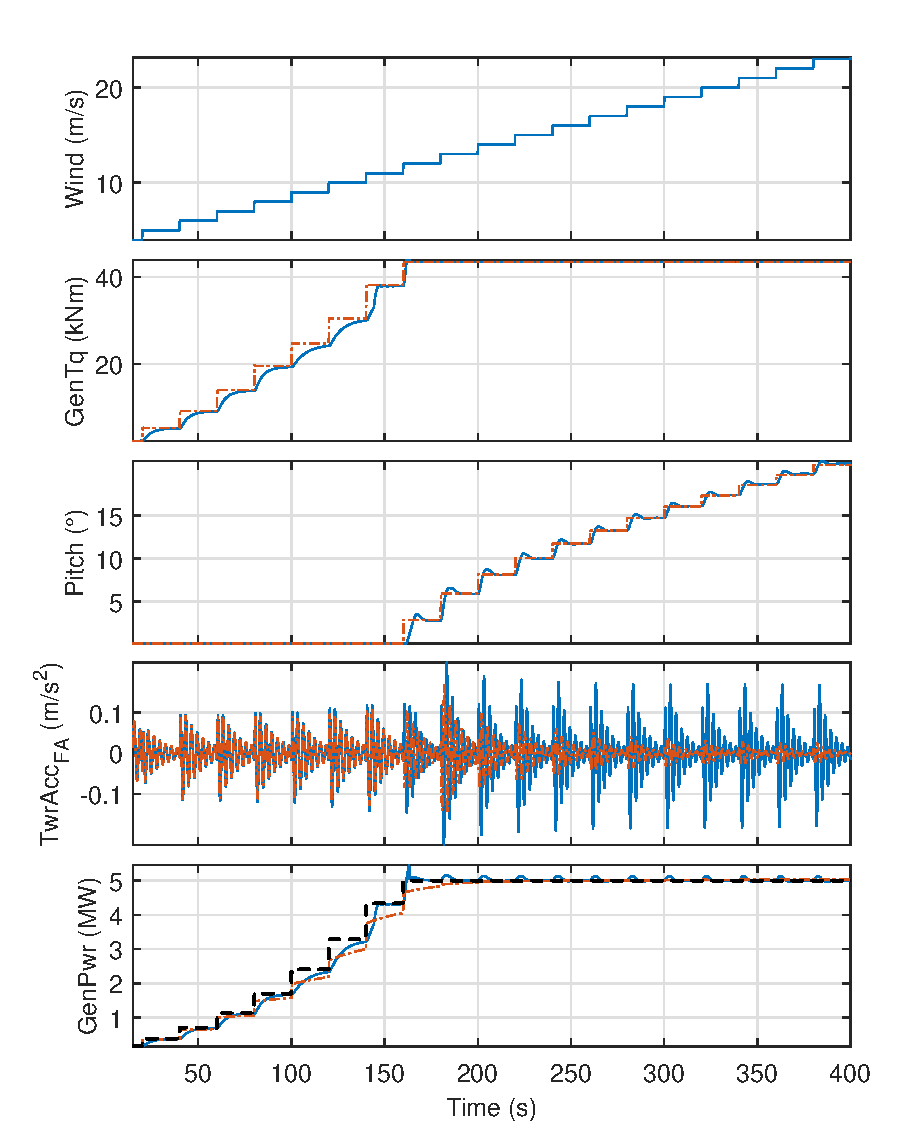
\includegraphics[width=0.495\textwidth, trim={0.cm 0cm 0cm 0.5cm}, clip]{figures/Figures_ADi/cmpCtrlTimeDomain_All_RefSimulinkClosedLoop_beta.eps}}\hfill
    \subfloat[Turbulent wind, mean CPU time MPC 9.88$\cdot 10^{-4}$\,s]{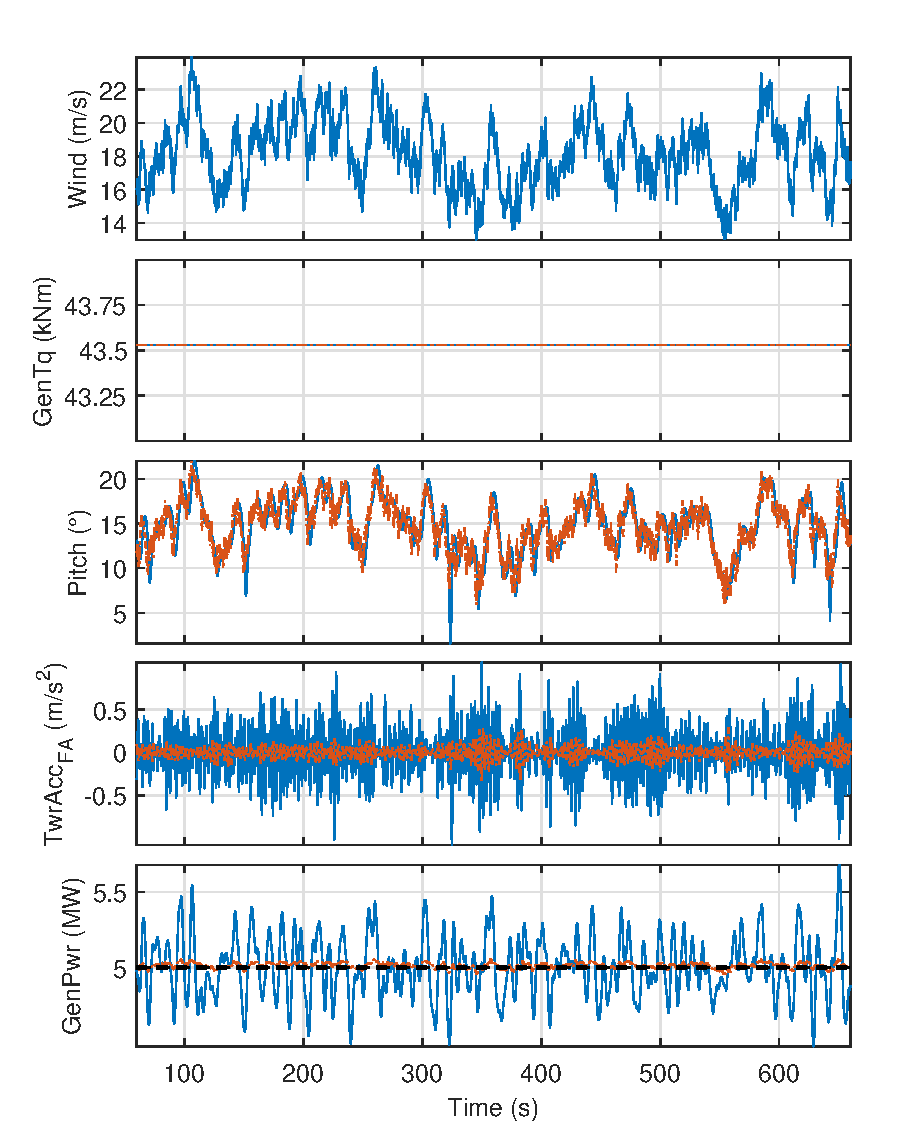
\includegraphics[width=0.495\textwidth,trim={0.cm 0cm 0cm 0.5cm}, clip]{figures/Figures_ADi/cmpCtrlTimeDomain_All_RefSimulinkClosedLoopNTW18_beta.eps}}\hfill
    %\subfloat[blc blc]{\includegraphics[width=0.31\textwidth]{figures/twoTurbinesGreedyOpt_2d.eps}}
    \caption[Controller comparison on qLPV model Mdl2: baseline PI vs.\ qLMPC for stepped wind sweep and turbulent wind.]{Controller comparison on qLPV model Mdl2: baseline PI (\mlBlue) vs.\ qLMPC (\mlOrange) for stepped wind sweep and turbulent wind (18~m/s mean, turbulence class B) with power reference~(\mlBlackDashed). Displayed signals: freestream wind speed, control inputs, tower fore-aft
        accelerations, and power output.}
    \label{fig:CtrlCmpMdlSweep}
\end{figure}
%
In the first test case, the wind speed is increased stepwise from 4\,m/s to 23\,m/s in steps with a duration of 20\,s, resulting in a simulation time of 400\,s, with the first 15\,s discarded as a transient. In the second scenario, 660\,s of turbulent wind with a mean speed of 18\,m/s and turbulence class B of the International Electrotechnical Commission (IEC) is used to assess controller performance under realistic wind conditions, and the first 60\,s are left out of the analysis. The results are shown in Figure~\ref{fig:CtrlCmpMdlSweep}.
%

Figure~\ref{fig:CtrlCmpMdlSweep}(a) shows the controller comparison for the stepped wind sweep covering nearly the entire operating range. In below-rated wind conditions, the two controllers achieve comparable performance. In above-rated wind conditions, however, predictive pitch control considerably reduces tower fore-aft acceleration and power variance. Overall, the standard deviation ratios for the tower fore-aft acceleration and power tracking error are 1.74 and 1.14 (corresponding to variance reduction factors of 3.04 and 1.29), as shown in Table~\ref{tab:ControllerComparisonMerged}.
%
Figure~\ref{fig:CtrlCmpMdlSweep}(b) shows results for the turbulent wind. The improvements over the baseline PI are even more pronounced than in the stepped sweep case. For the tower fore-aft acceleration and power tracking error, the qLMPC yields standard deviation ratios of 4.14 and 11.35 (equivalent to variance reduction factors of 17.14 and 128.88), see Table~\ref{tab:ControllerComparisonMerged}.

The QP is solved using a linear complementarity problem formulation with Lemke's algorithm \cite{cisneros2020velocity}, warm-started with the solution of the previous sample, which enables fast computation, as real-time capability is a critical requirement for online optimization-based control. Of the 50001 controller cycles at a sampling time of 8\,ms needed for the 400\,s simulation time of the stepped wind sweep, only one cycle exceeded the sampling time and only 13 exceeded 2\,ms. The mean CPU time was approximately 1\,ms, as shown in the subplot captions of Figure~\ref{fig:CtrlCmpMdlSweep}. These measurements were obtained in MATLAB R2023a on an Intel Core i7-11850H (2.5\,GHz, 8 cores) running Windows 10. Note that for deployment on a physical turbine, a fallback strategy would be required to handle the rare cases where the solver exceeds the sampling time. This was not implemented in this proof-of-concept, but several options exist, such as blending the last available qLMPC solution with the output of the PI feedback controller.

The improvements regarding the reduction of tower acceleration and power variance come at the price of higher pitch activity. As summarized in Table~\ref{tab:ControllerComparisonMerged}, the standard deviation of the blade pitch rate increases by a factor of approximately 3.6 in the stepped wind sweep and 3.7 in the turbulent wind case, and that of the generator torque rate by a factor of approximately 2.6 in the stepped wind sweep. In the turbulent wind case, both controllers operate at rated generator torque throughout, resulting in zero torque rate standard deviation.

\begin{table}[t]
    \centering
    \caption[Standard deviation comparison with qLPV model Mdl2: Baseline PI vs.\ qLMPC for stepped wind sweep and turbulent wind.]%
    {Standard deviation comparison with qLPV model Mdl2: Baseline PI vs.\ qLMPC for stepped wind sweep and turbulent wind (18\,m/s mean, IEC class B).
        The standard deviations obtained with the PI controller are divided by those obtained with the qLMPC;
        quotients above~1 indicate improvement. Ratios are computed from unrounded values.}
    \label{tab:ControllerComparisonMerged}
    \begin{tabular}{l rr}
        \toprule
        {Standard Deviation of} & {Stepped wind sweep} & {Turbulent wind} \\
        {Signal (unit)} & \multicolumn{2}{c}{std PI / std qLMPC = ratio} \\
        \midrule
        Tower fore-aft acc. (m/s$^2$)  & $0.0597 / 0.0342 \approx 1.74$ & $0.3110 / 0.0751 \approx 4.14$  \\
        Power tracking error (kW)& $176.01 / 154.95 \approx 1.14$ & $201.12 / 17.72 \approx 11.35$  \\
        Generator torque rate (kNm/s)  & $0.56 / 1.47 \approx 0.38$     & $0.00 / 0.00 = {-}$     \\
        Blade pitch rate (\textdegree/s)  & $0.21 / 0.76 \approx 0.28$     & $1.21 / 4.44 \approx 0.27$   \\
        \bottomrule
    \end{tabular}
\end{table}

As more improvement in power variance was observed for the above-rated turbulent wind, the following discussion focuses on this case. In the results above, the pitch command increments are penalized, but the pitch rate state is not, and the pitch rate limit of 13\textdegree/s is relatively high compared to the 8\textdegree/s of the NREL 5MW reference turbine \cite{jonkman2009definition}. Figure~\ref{fig:CtrlCmpRates} shows the results of six test runs with different pitch rate limits on the plant without the wind filters: three with the baseline PI controller and three with the qLMPC algorithm.
\begin{figure}[h]
    \subfloat[Baseline PI controller]{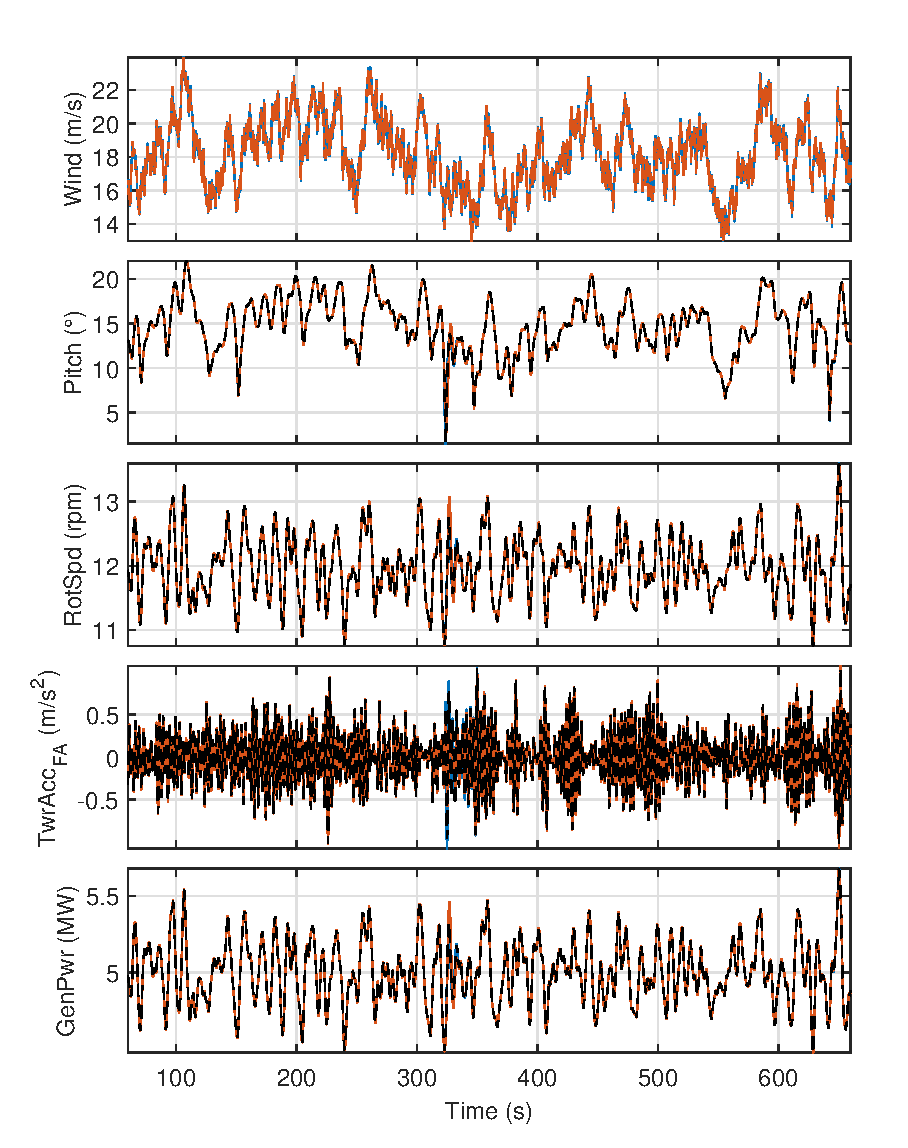
\includegraphics[width=0.495\textwidth,trim={0.cm 0cm 0cm 0.65cm}, clip]{figures/figDirConstr1/cmpTimeDomain_All5PINewLim_NoFilt.eps}}\hfill
    \subfloat[qLMPC algorithm]{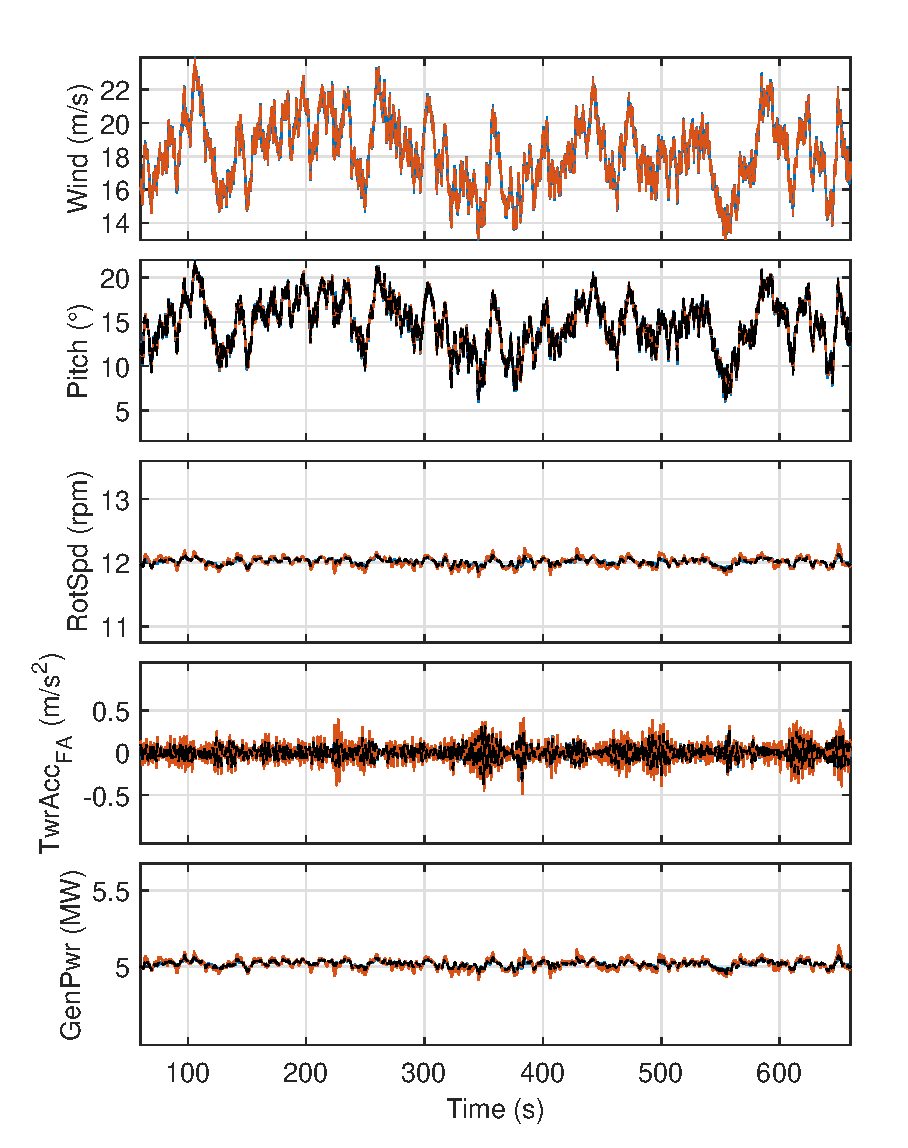
\includegraphics[width=0.495\textwidth,trim={0.cm 0cm 0cm 0.65cm}, clip]{figures/figDirConstr1/cmpTimeDomain_All5MPCNewLim.eps}}\hfill
    \caption[Controller comparison on qLPV model Mdl2: baseline PI and qLMPC with different pitch rate limits.]{Controller comparison on qLPV model Mdl2: baseline PI and qLMPC with different pitch rate limits for turbulent wind (18\,m/s mean, turbulence  class B), both controllers on the plant without the wind filters. Rate limits: Standard 8\textdegree/s~(\mBlack), high 13\textdegree/s~(\mlBlue), and low 4\textdegree/s~(\mlOrange). Displayed signals: freestream wind speed, pitch, states, and power.}
    \label{fig:CtrlCmpRates}
\end{figure}
The effect of different pitch rate limits on the PI controller is depicted in Figure~\ref{fig:CtrlCmpRates}(a), and on the qLMPC design in Figure~\ref{fig:CtrlCmpRates}(b). The selected pitch rate limits of 4\textdegree/s, 8\textdegree/s, and 13\textdegree/s represent a range from conservative to highly responsive actuator capabilities. They were chosen to explore both realistic hardware limitations and the potential performance gains of faster actuation. The signals shown for both control algorithms are the wind speed, collective blade pitch angle, rotor speed, fore-aft tower acceleration, and generator power. The generator torque does not change in this above-rated test case and is hence not shown. Under baseline PI control, the pitch rate limit has almost no effect: the standard deviations of the tower fore-aft acceleration, the rotor speed and the power tracking error change by at most about 1\,\% between 4\textdegree/s and 13\textdegree/s. The PI controller reaches the respective rate limit only occasionally and exceeds 4\textdegree/s during less than 1\,\% of the time, as the rotor acts as a filter in this pure feedback design. In contrast, the qLMPC exceeds 4\textdegree/s during more than a third of the time if allowed, and shows a considerable difference between the 4\textdegree/s rate limit and the two higher rates. Allowing a pitch rate of 8\textdegree/s or faster improves rotor speed regulation and reduces the standard deviations of rotor speed and power by a factor of about 1.6 compared to the 4\textdegree/s limit. However, it also leads to higher pitch activity. The qLMPC reduces the variance of rotor speed, tower fore-aft movement, and power output compared to the PI controller for all rate limits, even at a 4\textdegree/s rate limit, where the standard deviations of the tower fore-aft acceleration and of the power tracking error are still reduced by factors of 2.58 and 6.42. The qLMPC benefits from higher pitch rates, as a faster pitch response enables better disturbance rejection, e.g.\ of gusts. The trade-off between actuator activity on the one hand and load reduction and smoother power output on the other is a design decision, which may also vary over the turbine's lifetime as the pitch bearings age. 
%
Figure~\ref{fig:CtrlCmpFilt2} shows both controllers on the plant with the wind filters introduced in Section~\ref{sec:qLPVModelVerificationwithFAST0}, which imitate the averaging effect of a wind field acting on the whole rotor instead of a single-point wind speed. 
\begin{figure}[h]
    \centering
    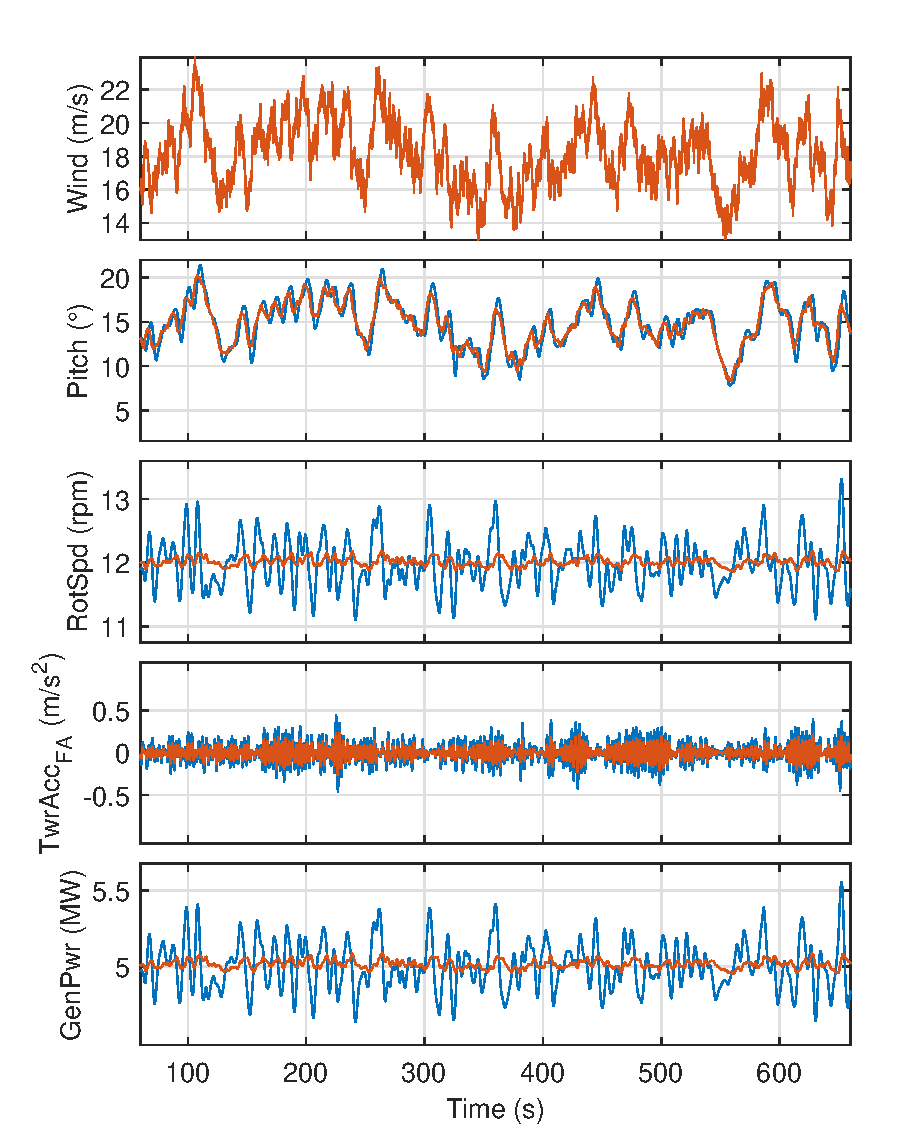
\includegraphics[width=0.495\textwidth,trim={0.cm 0cm 0cm 0.7cm}, clip]{figures/figDirConstr1/cmpTimeDomain_All5PIvsMPC_Filt.eps}
    \caption[Controller comparison on qLPV model Mdl2 with filtered wind: baseline PI and qLMPC.]{Controller comparison on qLPV model Mdl2 with filtered wind: baseline PI (\mlBlue) and qLMPC (\mlOrange), qLMPC and Mdl2 with rotor-effective wind filters for turbulent wind (18\,m/s mean, turbulence class B), pitch rate limit 13\textdegree/s. Displayed signals: freestream wind speed, pitch, states, and power.}
    \label{fig:CtrlCmpFilt2}
\end{figure}
The standard deviations of the pitch derivative, the rotor speed, the tower fore-aft acceleration and the power tracking error for Figures~\ref{fig:CtrlCmpRates} and~\ref{fig:CtrlCmpFilt2} are summarized in Table~\ref{tab:stddev_unified}.

\begin{table}[htbp]
    \centering
    \setlength{\tabcolsep}{4.5pt}
    \caption[Standard deviations: Baseline PI and qLMPC for turbulent wind and different pitch rate limits.]%
    {Standard deviations: Baseline PI and qLMPC for turbulent wind and different pitch rate limits
        (\textdegree/s). Columns 4, 8, 13: plant without rotor-effective wind filters. Last column: plant
        with filters, qLMPC scheduled with the filtered wind. Brackets: PI value at 8\textdegree/s without
        filters divided by the entry; for the filtered qLMPC, the filtered PI value is used instead.}
    \label{tab:stddev_unified}
    \begin{tabular}{ll rrrr}
        \toprule
        & & \multicolumn{4}{c}{Rate limit (\textdegree/s)} \\
        \cmidrule(lr){3-6}
        %Ctrl. & Signal & 4 & 8 & 13 & 13, filt. \\
        Ctrl. & Signal & low: 4 & standard: 8 & high: 13 & filt. wind: 13 \\
        \midrule
        \multirow{4}{*}{PI}
        & Tower acc.\ (m/s$^2$)      & 0.3076 (1.01) & 0.3108 (1.00) & 0.3110 (1.00) & 0.1300 (2.39) \\
        & Power error (kW)           & 202.04 (1.00) & 201.22 (1.00) & 201.12 (1.00) & 159.33 (1.26) \\
        & Rotor speed (rpm)          & 0.4830 (1.00) & 0.4810 (1.00) & 0.4808 (1.00) & 0.3812 (1.26) \\
        & Pitch rate (\textdegree/s) & 1.13 (1.04)   & 1.18 (1.00)   & 1.21 (0.98)   & 0.71 (1.66) \\
        \midrule
        \multirow{4}{*}{qLMPC}
        & Tower acc.\ (m/s$^2$)      & 0.1204 (2.58) & 0.0813 (3.82)  & 0.0751 (4.14)  & 0.0723 (1.80) \\
        & Power error (kW)           & 31.35 (6.42)  & 19.56 (10.29)  & 17.72 (11.35)  & 27.40 (5.82) \\
        & Rotor speed (rpm)          & 0.0743 (6.47) & 0.0464 (10.37) & 0.0422 (11.40) & 0.0655 (5.82) \\
        & Pitch rate (\textdegree/s) & 2.91 (0.41)   & 4.07 (0.29)    & 4.44 (0.27)    & 0.54 (1.31) \\
        \bottomrule
    \end{tabular}
\end{table}

The same axis limits as in Figure~\ref{fig:CtrlCmpRates}(a) are used in Figure~\ref{fig:CtrlCmpRates}(b) to highlight the improvements possible with the qLMPC and in Figure~\ref{fig:CtrlCmpFilt2} to visualize the smoothing effect of the filters on both PI and qLMPC. On the filtered plant, the largest pitch rate is 2.5\textdegree/s for the PI controller and 2.6\textdegree/s for the qLMPC, although the pitch rate limit is 13\textdegree/s, so all rate limits from 3\textdegree/s upwards are inactive and give identical results. The filters alone reduce the standard deviations of the PI controller by a factor of 2.39 for the tower fore-aft acceleration and 1.26 for the rotor speed and the power tracking error. On the filtered plant, the qLMPC still reduces the standard deviations of the tower fore-aft acceleration, the rotor speed and the power tracking error by factors of 1.80, 5.82 and 5.82 compared with the PI controller, but considerably less than without the filters. At the same time, the pitch activity changes fundamentally: with the filtered wind, the standard deviation of the qLMPC pitch rate is 0.54\textdegree/s, which is even below the 0.71\textdegree/s of the PI controller, whereas without the filters the qLMPC requires 4.44\textdegree/s, more than three times as much as the PI controller. A large part of both the pitch activity and the improvement of the qLMPC without the filters is therefore caused by the high-frequency fluctuations of the single-point wind speed. These fluctuations excite the plant strongly, so that the PI controller, which only reacts to the resulting rotor speed changes, leads to large oscillations, while the qLMPC, which knows the wind speed exactly, compensates them with fast pitch action. A real rotor averages these fluctuations out. The unfiltered case nevertheless shows the benefit of high pitch rates for fast disturbances and represents a worst case regarding the demanded pitch activity.
%
All ratios in this table relate the two controllers on the same plant, with one exception: the last column of the PI block relates the PI on the plant with the wind filters to the PI on the plant without the filters and thus shows the effect of the filters themselves.

\subsubsection{Results on FAST}\label{subsubsec:qLMPCFASTresults}

Figure~\ref{fig:CtrlCmpFAST} shows the baseline PI controller, the original qLMPC, and the notch filter and smooth designs of Section~\ref{sec:qLMPCFAST} on FAST for the stepped wind sweep and the turbulent 18\,m/s wind field of Section~\ref{quasiLPVMPCResults}, with a pitch rate limit of 13\textdegree/s. The standard deviations are summarized in Table~\ref{tab:CtrlComparisonFAST}, with the ratio of the baseline PI value to the value of the respective controller in parentheses.
%
\begin{figure}[htbp]
    \subfloat[Stepped wind sweep.]{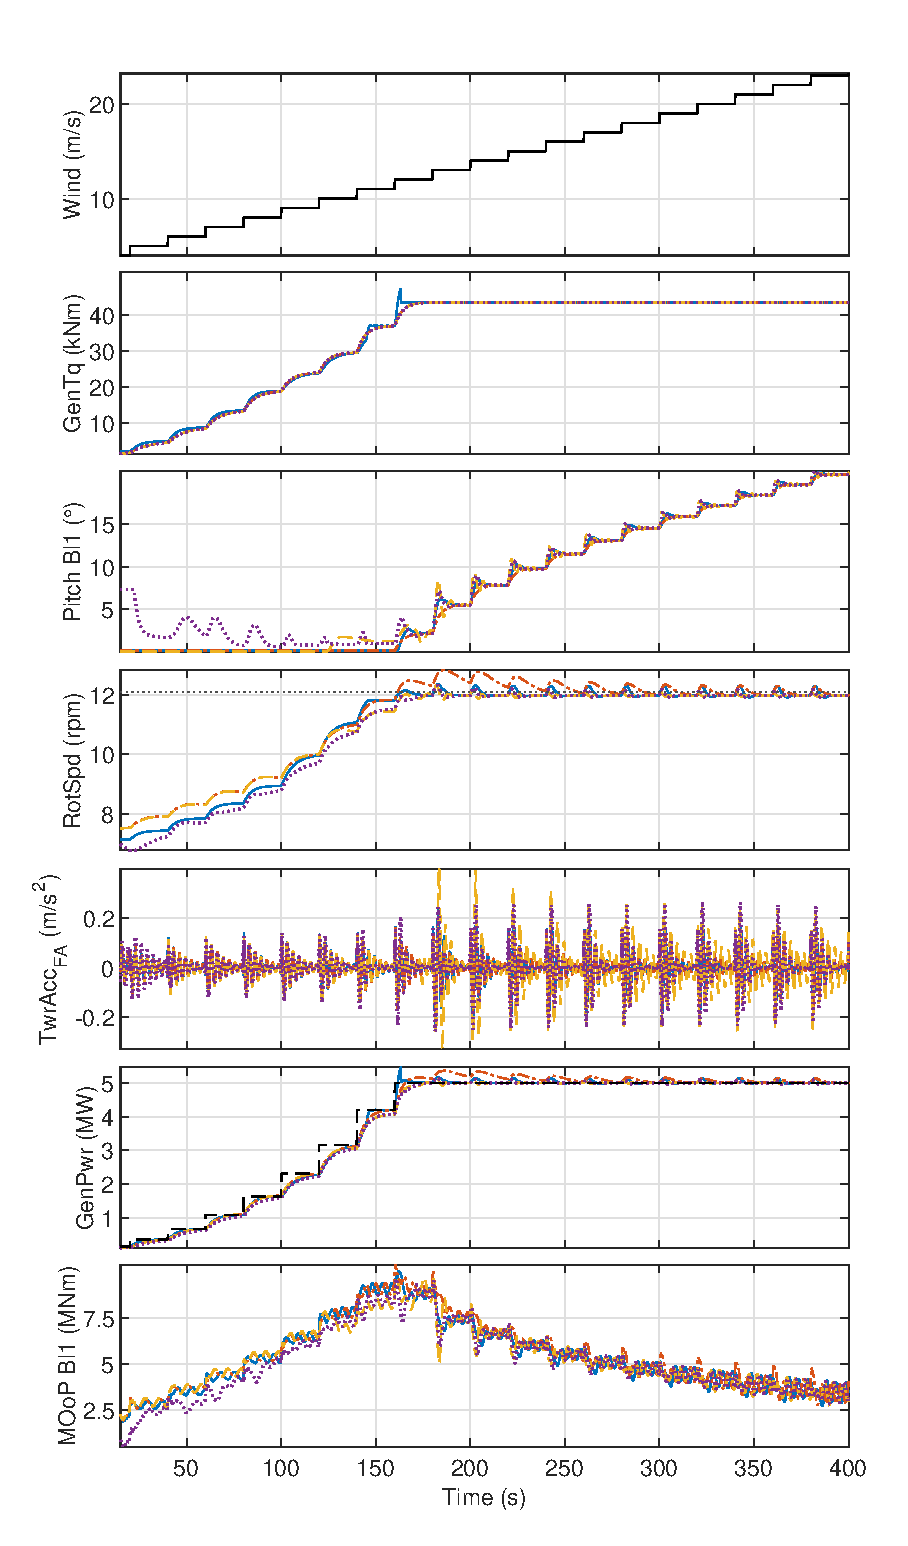
\includegraphics[width=0.495\textwidth,trim={0.cm 0cm 0cm 0.9cm}, clip]{figures/figDirFASTthesis/cmpCtrlFASTthesis_Sweep_PI_beta_flapNotch_flapNotchSmooth12.eps}}\hfill
    \subfloat[Turbulent wind, 18~m/s mean, turbulence class~B.]{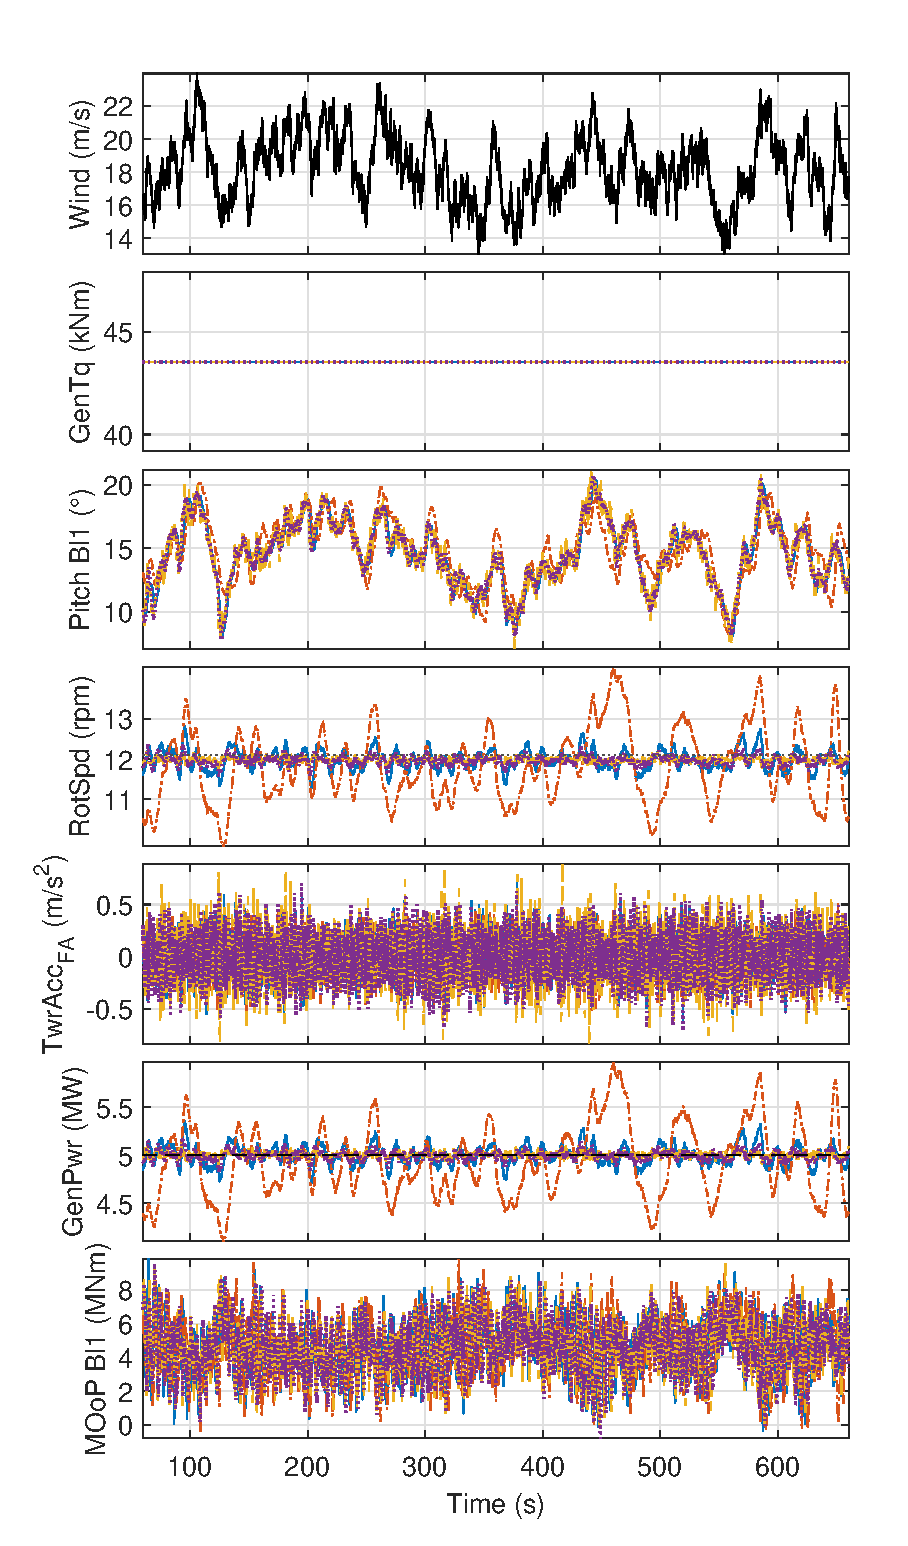
\includegraphics[width=0.495\textwidth, trim={0.cm 0cm 0cm 0.9cm}, clip]{figures/figDirFASTthesis/cmpCtrlFASTthesis_NTM18B_PI_beta_flapNotch_flapNotchSmooth12.eps}}
    \caption[Controller comparison on FAST: baseline PI, original qLMPC, and the qLMPC designs for FAST]{Controller comparison on FAST: baseline PI controller (\mlBlue), original qLMPC (\mlOrange), notch filter design (\mlYellow), and smooth design (\mlPurple) for the stepped wind sweep and turbulent wind (18\,m/s mean, turbulence class B), pitch rate limit 13\textdegree/s. Displayed signals: freestream wind speed, generator torque, blade 1 pitch angle, rotor speed, tower fore-aft acceleration, generator power with its reference (black dashed line), and blade 1 root out-of-plane moment.}
    \label{fig:CtrlCmpFAST}
\end{figure}
In the stepped wind sweep, shown in Figure~\ref{fig:CtrlCmpFAST}(a), the differences between the controllers are small. The original qLMPC, depicted in orange, slightly outperforms the baseline PI controller, shown in blue, with a decrease of 8\% in the standard deviation of the tower fore-aft acceleration and of 4\% in those of the power tracking error and the rotor speed. This is achieved with smoother pitching, so that all four values show an improvement. The two other qLMPC designs, which were developed to address the issues in turbulent wind, show no overall improvement for the stepped wind sweep. Only the standard deviation of the rotor speed of the notch filter design decreases slightly, but due to the much more aggressive pitching, this does not translate into a lower standard deviation of the power tracking error. Presumably, these performance decreases result from the rotor-effective wind filter, which delays the scheduling wind speed although the wind steps act on the whole rotor area at once. This is particularly noticeable for the smooth design, whose pitch angle deviates from zero below rated wind speed.

In the turbulent wind, the original qLMPC, which performs very well on Mdl2 for both test cases and reasonably well on FAST for the stepped wind sweep test case, fails on FAST: the rotor speed varies between 10\,rpm and 14.3\,rpm, and the standard deviations of the rotor speed and of the power tracking error are 3.7 and 3.6 times those of the baseline PI controller. The notch filter design reduces these standard deviations by factors of 3.8 and 3.3 compared with the baseline PI controller, and the smooth design by factors of 2.1 and 2.0. This is less than the factor of 11.4 on Mdl2 (Table~\ref{tab:stddev_unified}), but still a considerable smoothing of the power output. In contrast to Mdl2, however, the tower fore-aft acceleration is not reduced but increased, by 35\% for the notch filter design and 16\% for the smooth design, and the tower base DEL increases by 27\% and 12\%; for the wind of the second verification set and a pitch rate limit of 8\textdegree/s, the increases are 33\% and 16\%, see Section~\ref{subsec:ComparisonWindTurbineControlDesigns}. The pitch rate standard deviation is 5.9 times that of the baseline PI controller for the notch filter design and 2.4 times for the smooth design. The adaptations thus make the qLMPC applicable to FAST and retain a large part of the power smoothing in turbulent wind, but not the reduction of the tower loads achieved on Mdl2. The smooth design trades part of the power smoothing for considerably less pitch activity and a smaller increase of the tower loads.

\begin{table}[h]
    \centering
    \caption[Controller comparison on FAST for stepped wind sweep and turbulent wind.]{Controller comparison on FAST v8.16 for the stepped wind sweep and turbulent wind (18\,m/s mean, turbulence class B), pitch rate limit 13\textdegree/s: standard deviations of the tower fore-aft acceleration, the power tracking error, the rotor speed, and the (collective) pitch rate. In parentheses the ratio baseline PI/controller; values above 1 indicate an improvement.}
    \label{tab:CtrlComparisonFAST}
    \begin{tabular}{ll rrrr}
        \toprule
        & & & \multicolumn{3}{c}{qLMPC} \\
        \cmidrule(lr){4-6}
        Wind & Signal & Baseline PI & original & notch filter & smooth \\
        \midrule
        \multirow{4}{*}{Sweep}
        & Tower acc.\ (m/s$^2$)      & 0.0558 & 0.0516 (1.08) & 0.0826 (0.67) & 0.0684 (0.82) \\
        & Power error (kW)           & 141.85 & 136.15 (1.04) & 144.65 (0.98) & 156.66 (0.91) \\
        & Rotor speed (rpm)          & 1.6977 & 1.6264 (1.04) & 1.4993 (1.13) & 1.7719 (0.96) \\
        & Pitch rate (\textdegree/s) & 0.22   & 0.12 (1.76)   & 0.50 (0.44)   & 0.39 (0.55) \\
        \midrule
        \multirow{4}{*}{Turbulent}
        & Tower acc.\ (m/s$^2$)      & 0.1712 & 0.1689 (1.01) & 0.2310 (0.74) & 0.1990 (0.86) \\
        & Power error (kW)           & 59.60  & 214.42 (0.28) & 17.90 (3.33)  & 29.18 (2.04) \\
        & Rotor speed (rpm)          & 0.2460 & 0.9035 (0.27) & 0.0653 (3.77) & 0.1145 (2.15) \\
        & Pitch rate (\textdegree/s) & 0.49   & 0.68 (0.72)   & 2.87 (0.17)   & 1.18 (0.41) \\
        \bottomrule
    \end{tabular}
\end{table}

%\input{figures/figDirFASTthesis/resultsFASTthesis_NTM18B_PI_beta_flapNotch_flapNotchSmooth12}

The application of the proposed velocity-based qLMPC concept to the qLPV model considerably reduces tower movements and power output fluctuations. As noted at the start of this section, DEL reduction is not directly a qLMPC objective. On FAST, with the adaptations of Section~\ref{sec:qLMPCFAST}, the qLMPC still reduces the power fluctuations, but the tower loads increase, as shown above and in the comparison with the other controllers in Section~\ref{subsec:ComparisonWindTurbineControlDesigns}.

This study shows that considerable performance improvements are possible without model mismatch, and this best-case scenario underlines the potential of the algorithm. However, even the model mismatch between the carefully tuned qLPV model and FAST deteriorates the performance of the original qLMPC. With the adaptations for FAST, a large part of the power smoothing is retained, but the tower loads increase, which shows the sensitivity of the qLMPC to model mismatch. Moreover, the performance improvement comes at the cost of requiring accurate wind information, obtained either through expensive sensors such as lidars or through wind speed estimation. A purely feedback-based improvement over standard collective pitch control is individual pitch control, which uses blade root moments and the rotor azimuth position as additional feedback signals and is already widely deployed in commercial turbines. This approach has been extensively investigated in both theoretical studies and field tests and has proven to be an effective strategy to further reduce mechanical loads, either as an alternative or in addition to MPC. While its primary focus is on reducing blade loads, a slight reduction in tower loads is also possible, as will be discussed in the next section.

\section{Individual Pitch Control Design and Application}\label{section:Individal Pitch PI Control} 
IPC is a control technique designed to mitigate cyclic loads on wind turbine blades by independently adjusting the pitch angle of each blade. These cyclic loads primarily result from wind shear, i.e., the increase in wind speed with altitude due to reduced surface friction farther from the ground. Additional causes of load imbalances include yaw misalignment, rotor tilt, turbulence, gusts, and tower shadow effects. These effects lead to asymmetric aerodynamic loading, which induces bending moments perpendicular to the rotor plane at the blade roots, referred to as out-of-plane bending moments. They occur at specific multiples of the rotor's rotational frequency, commonly referred to as $n\text{P}$ frequencies, e.g., $1\text{P}$ and $2\text{P}$ correspond to once and twice per revolution, respectively. These periodic loads accumulate fatigue damage in the blades and, via the resulting tilt and yaw moments, in the hub, shaft and nacelle. In addition, they can excite the turbine's natural structural modes if an $n\text{P}$ frequency coincides with a natural frequency, which further accelerates fatigue and reduces component lifespan.

The turbine blade deformation can be decomposed into three primary directions relative to the blade itself: flapwise, which is perpendicular to the rotor plane if the blade is not pitched, edgewise within the rotor plane, and torsional twisting along the blade's axis. The flapwise and edgewise blade root bending moments are measured directly, for example via strain gauges, and transformed into moments within and perpendicular to the rotor plane using the current pitch angle. The out-of-plane moments serve as feedback for IPC. IPC suppresses these loads by transforming the blade root moments from the rotating into the non-rotating coordinate system, computing tilt and yaw pitch demands with a controller, and transforming these back into the rotating frame before adding them to the blade pitch signals.

The block diagram in Figure~\ref{fig:BlockIPC} illustrates the IPC architecture. It shows the main components of the system, including the controller, which is divided into the power controller and the IPC controller, highlighted in red. The figure also displays the NREL 5MW wind turbine, the pitch actuator, and the torque actuator.
\begin{figure}[ht]
    \centering
    \includegraphics[width=0.9\textwidth,trim={0 0cm 0cm 0.005cm},clip]{figures/Figures_ADi/turbineCtrlBetaIPCcl.pdf}
    \caption[Block diagram of IPC enhancing baseline power control.]{Block diagram of IPC enhancing baseline power control: the power control sets the collective pitch and generator torque references. In the IPC block (red), MBC transforms the blade root moments $M_{yci}$ into the tilt and yaw moments $M_c$ and $M_s$, which are scaled with $k_M$ and the PI gains $K_{\text{IPC}}$. Its outputs are transformed back into individual pitch demands $\beta_{i,\text{IPC}}$ added to $\beta_{0,\text{ref}}$.}
    \label{fig:BlockIPC}
\end{figure}
%
In this work, PI controllers are utilized rather than full PID architectures. This choice is consistent with the NREL 5MW baseline controller provided in FAST. Furthermore, a joint optimization including a derivative gain, see Section~\ref{subsection: IPCOptCriteria}, reduced the blade DEL by only 2.3 percentage points more, at almost twice the pitch activity, which would increase actuator wear.

The three blade pitch angles $\beta_1$, $\beta_2$, and $\beta_3$ are the outputs of the pitch actuators corresponding to the references $\beta_{1,\text{ref}}$, $\beta_{2,\text{ref}}$, and $\beta_{3,\text{ref}}$. These references are the sum of the collective reference signal $\beta_{0,\text{ref}}$ from the power controller and the respective IPC adjustments $\beta_{1,\text{IPC}}$, $\beta_{2,\text{IPC}}$, and $\beta_{3,\text{IPC}}$.
%
As before, the power control loop sets the collective pitch reference $\beta_{0,\text{ref}}$ as well as the generator torque reference $T_{g,\text{ref}}$, based on feedback from the generator speed $\omega_g$.
%
The IPC adjustments are derived from the out-of-plane blade root bending moments $M_{yc1}$, $M_{yc2}$, and $M_{yc3}$ and the position of the first blade $\theta_{r}$, also called the rotor position or rotor azimuth. The blade root moments are transformed from the rotating into the non-rotating coordinate system by a multiplication with the matrix $\frac{2}{3}V_{\theta_{r}}^{T}$. The back-transformation before applying the control signals to the rotating blades is done by a multiplication with the matrix $V_{\theta_{r}}$. The underlying method for these coordinate transformations, known as multiblade coordinate transformation, and the design of $V_{\theta_{r}}$ are explained in detail below.

% (\texttt{RootMyb1} and \texttt{RootMyc1} for the first blade)

\subsection{Multiblade Coordinate Transformation} \label{sec:MBC}
Multiblade coordinate transformation (MBC) enables the conversion of dynamic loads from the rotating coordinate system, defined by the azimuth angle $\theta_{r}$, to a fixed tower coordinate system. Specifically, load components at the rotation frequency are transformed via the MBC to quasi-static loads. Hence, MBC allows for a more accurate assessment of the loads acting on the turbine tower and other non-rotating components. 

Note that the blade root moments measured by strain gauges are expressed in the blade coordinate system, which rotates with the pitch angle: the flapwise moment $M_{ybi}$ acts perpendicular to the chord line and the edgewise moment $M_{xbi}$ along it. For IPC, the moments perpendicular to the rotor plane are required. These out-of-plane moments $M_{yci}$ are obtained by rotating the flapwise and edgewise moments by the pitch angle $\beta_i$ of the respective blade into the coned coordinate system, which does not rotate with the pitch \cite{jonkman2005fast}:
\begin{equation} \label{eq:MoopFAST}
    M_{yci} = M_{ybi} \cos(\beta_i) - M_{xbi} \sin(\beta_i), \quad i = 1, 2, 3.
\end{equation}
For zero pitch, the out-of-plane moment thus equals the flapwise moment, while with increasing pitch angle, an increasing part of the edgewise moment contributes to the out-of-plane moment. FAST provides both the moments in the blade coordinate system and the out-of-plane moments in the coned coordinate system as outputs. For convenience, the out-of-plane moments $M_{yci}$ provided by FAST are used directly as feedback signals for IPC in this work.

Applying MBC to convert the rotating blade root out-of-plane moments into a fixed coordinate system for a three-bladed wind turbine results in the matrix notation 

\begin{equation} \label{eq:MBC}
    \left[ \begin{array}{c}
        M_0\\
        M_c\\
        M_s
    \end{array} \right] = \frac{2}{3}
    \left[ \begin{array}{ccc}
        1/2 & 1/2 & 1/2\\
        \cos(\theta_{r}) & \cos(\theta_{r} + \frac{2\pi}{3}) & \cos(\theta_{r} + \frac{4\pi}{3})\\
        \sin(\theta_{r}) & \sin(\theta_{r} + \frac{2\pi}{3}) & \sin(\theta_{r} + \frac{4\pi}{3})
    \end{array} \right]
    \left[ \begin{array}{c}
        M_{yc1}\\
        M_{yc2}\\
        M_{yc3}
    \end{array} \right], 
\end{equation}
with $M_{yci}$ as the out-of-plane root moment of the $i$-th blade as inputs and the moments in the non-rotating system as outputs, with these moments being the symmetric load moment $M_0$, tilt moment $M_c$ and yaw moment $M_s$, as visualized in Figure~\ref{fig:BlockIPC}. The tilt and yaw moments are used to calculate two cyclic control signals $q_c$ and $q_s$, i.e., $\beta_c$ and $\beta_s$ for IPC. 
The control signal $q_i$ of the $i$-th blade is calculated via the second and third columns of the inverse MBC transformation, i.e., the inverse of the matrix from Equation~\eqref{eq:MBC} %, is then used to calculate 
\begin{equation} \label{eq:inverseMBC}
    \left[ \begin{array}{c}
        q_1\\
        q_2\\
        q_3
    \end{array} \right] = 
    \underbrace{\left[ \begin{array}{ccc}
            \cos(\theta_{r}) &  \sin(\theta_{r})\\
            \cos(\theta_{r} + \frac{2\pi}{3}) &  \sin(\theta_{r} + \frac{2\pi}{3})\\
            \cos(\theta_{r} + \frac{4\pi}{3}) &  \sin(\theta_{r} + \frac{4\pi}{3})
        \end{array} \right]}_{V_{\theta_{r}}}
    \left[ \begin{array}{c}
        q_c\\
        q_s
    \end{array} \right],
\end{equation}
where the signal $q_i$ denotes $\beta_{i,\text{IPC}}$ in IPC for the $i$-th blade. %In Section~\ref{sec:CombinedIPC-TrailingEdgeFlapControl} the same matrix multiplication is once again applied to the $i$-th flap.
Note that the transpose of the matrix $V_{\theta_{r}}$ from Equation~\eqref{eq:inverseMBC}, multiplied by $2/3$, is equal to the last two rows of the MBC matrix, see also \cite{ossmann2017load}. In the context of this work, and as is common in related literature, see, e.g.,~\cite{he2018combined}, the tilt and yaw moments $M_c$ and $M_s$ are controlled via $q_c$ and $q_s$ independently, i.e., any remaining coupling following the MBC transformation between $q_c$ and $M_s$ as well as $q_s$ and $M_c$ is neglected. As the wind turbine dynamics can be approximated as a Linear Time-Invariant (LTI) system after transforming rotor blade dynamics into a fixed coordinate system, using MBC from Equation~\eqref{eq:MBC}, a simple, intuitive control approach is adopted. Two separate SISO controllers, one for the tilt and one for the yaw moment, are designed to reduce the transformed moments $M_c$ and $M_s$. In this work, the same controller parameters are used, resulting in two parameters to be tuned for this PI controller. Note that the moment $M_0$, the collective out-of-plane moment caused by the rotor thrust, is determined by the collective pitch angle set by the baseline power controller and is not used in the IPC controls.

\subsection{IPC Parameter Optimization} \label{subsection: IPCOptCriteria}
The primary objective of wind turbine control is to minimize the Levelized Cost of Energy (LCoE) by balancing the conflicting goals of maximizing power output while minimizing mechanical loads, particularly DELs on the tower and blades. This work leverages controller optimization criteria similar to the ones originally used by \cite{hoffmann2018load}, where a standard baseline wind turbine controller, comprising a generator torque and a CPC PI pitch controller, is augmented with an IPC PI pitch controller and tower damping. The optimization criteria in a multi-objective optimization were the minimization of blade and tower DELs, actuator activity, power tracking error, and the standard deviation of the generated power. However, as in \cite{dittmer2024combined}, only the minimization of the blade DEL is implemented in this work, and the other criteria are used as evaluation criteria. In the following study, the optimization and simulation environment presented in \cite{dittmer2024combined} was used, which uses OpenFAST~v3.2.1. As before, this software is referred to as FAST.
%
The IPC PI controller optimization presented in this thesis consists of two optimization steps for each pitch rate limit:
\begin{enumerate}
    \item In the first step, the proportional and integral gains of the IPC are optimized with the Nelder-Mead simplex algorithm implemented in MATLAB's \textit{fminsearch.m} to reduce the blade DEL. A joint optimization including the derivative gain, tried for a pitch rate limit of 8\textdegree/s, resulted in $K_{\text{D,IPC}} = 0.15$ and a blade DEL reduction 2.3 percentage points higher, but almost twice the pitch activity; therefore only PI controllers are used.
    \item In the second step, the sequential quadratic programming algorithm of MATLAB's \textit{fmincon.m} is started from this result and minimizes the same cost function subject to the constraint that the tower base DEL must not exceed the value obtained with the baseline controller only, i.e., without IPC, at the same pitch rate limit.
\end{enumerate}
For all steps of the controller tuning, the quality of an IPC controller is quantified via the decrease in blade root DEL. The cost function $J$ to be minimized in the optimization is the maximum of the DELs of the three blades:
\begin{equation} \label{eq:costFunIPC}
    J = \max_{i \in \{1,2,3\}} \left(\text{DEL}_{b_i,\text{IPC}}/\text{DEL}_{b_i,\text{baseline}}\right)
\end{equation} %\underset{\Delta u}{\text{minimize }}
with $\text{DEL}_{b_i,\text{IPC}}$ the DEL of the out-of-plane root moment $M_{yci}$ of blade~$i$ over a simulation run with IPC and $\text{DEL}_{b_i,\text{baseline}}$ the corresponding DEL with only the baseline controller active. In the optimization, the DELs are calculated with the W\"ohler exponents of 8 for the blades and 3 for the tower base DEL of the constraint, the values set in MCrunch that were also used for the optimization in \cite{dittmer2024combined}. All evaluation criteria below are calculated with the W\"ohler exponents of 10 for the blades and 4 for the tower, the values used by NREL and in \cite{hoffmann2018load}, so that $C_{\text{DEL},b}$ differs slightly from $J$.
%\subsection{Optimization and evaluation criteria}
To evaluate and quantify the impact of an IPC controller's performance, five additional criteria are calculated, previously used in \cite{hoffmann2018load} as optimization criteria in a multi-objective optimization approach: the tower DELs derived from the fore-aft bending moments at the base and at the top of the tower, the mean and standard deviation of the generated power and the additional power requirements of the actuator due to individual pitch control. The evaluation criteria can be summarized as below.

\subsubsection*{Load Criteria: Blade DEL $C_{\text{DEL},b}$ and tower DEL $C_{\text{DEL},t}$}
Reducing the blade DEL is the main incentive for using IPC to decrease the Power Spectral Density (PSD) at 1P. A reduction at the 1P frequency does not directly influence the tower base DEL. However, finding a controller that decreases the peak at 1P tends to also result in a lower PSD for a wider frequency range including the peak at 2P. Thus, a small decrease in the tower top DEL is also achieved although this criterion is not included in the objective function. In Section~\ref{sec:CombinedIPC-TrailingEdgeFlapControl} it will be discussed that decreasing the PSD at the 2P frequency via the flaps decreases the tower top DEL further. In addition to the tower base DEL $C_{\text{DEL},t,\text{Base}}$, the DEL of the tower top fore-aft bending moment $C_{\text{DEL},t,\text{Top}}$ is evaluated, which is affected directly by the rotor tilt moment. Both tower DELs are calculated with the Wöhler exponent of steel. 

The damage of blade~$i$ is calculated from the rainflow counts of its out-of-plane root moment $M_{yci}$ as
\begin{align*}
    \Tilde{D}_{b_i} &= \sum_{j} l_{b_i,j}\, S_{b_i,j}^{m_{\text{GFRP}}}
\end{align*}
with $l_{b_i,j}$ the number of cycles of the moment range $S_{b_i,j}$ and the W\"ohler exponent $m_{\text{GFRP}} = 10$ of the Glass Fiber Reinforced Polymer (GFRP) blades. Unlike the cost function $J$, which minimizes the largest of the three blade DELs, the blade criterion uses the sum of the damages of the three blades:
\begin{align*}
    C_{\text{DEL},b} &= \left(\sum_{i=1}^{3}\Tilde{D}_{b_i,\text{IPC}} \Big/ \sum_{i=1}^{3}\Tilde{D}_{b_i,\text{baseline}}\right)^{1/m_{\text{GFRP}}}
\end{align*}
with the damage ratio of the summed blade damages recorded with the two controllers for the same test case. As the DEL is proportional to the $m$-th root of the damage, $C_{\text{DEL},b}$ is the ratio of the blade DELs.

The tower criteria are calculated in the same way from the fore-aft bending moments at the tower base and at the tower top:
\begin{align*}
    C_{\text{DEL},t,\text{Base}} &= \left(\Tilde{D}_{t,\text{Base},\text{IPC}}/\Tilde{D}_{t,\text{Base},\text{baseline}}\right)^{1/m_{\text{Steel}}}, \quad
    C_{\text{DEL},t,\text{Top}} = \left(\Tilde{D}_{t,\text{Top},\text{IPC}}/\Tilde{D}_{t,\text{Top},\text{baseline}}\right)^{1/m_{\text{Steel}}},
\end{align*}
with the damages $\Tilde{D}_{t} = \sum_{j} l_{t,j}\, S_{t,j}^{m_{\text{Steel}}}$ of the respective moment, recorded with the IPC and with the CPC-PI controller for the same test case, and the W\"ohler exponent $m_{\text{Steel}} = 4$ of steel.

\subsubsection*{Power Criteria: Mean $C_{\bar{P}}$ and Standard Deviation $C_{\delta P}$}
As the annual energy production should not suffer from IPC, the generated power is compared as well. The power variance is important for the network stability, especially in small networks. It was found that the power production loss is at most 0.6\% close to rated wind speed and that the variance increases only slightly, so that both effects are negligible. Similarly to the DEL criteria, the power criteria are normalized by the results obtained with the CPC-PI controller
\begin{align*} %\label{eq:CP}
    C_{\bar{P}} =  \bar{P}_{\text{g,\text{IPC}}}/ \bar{P}_{\text{g,\text{baseline}}}  \quad\text{and}\quad C_{\delta P} =  \delta P_{g,\text{IPC}}/ \delta P_{g,\text{baseline}}.
\end{align*} 

\subsubsection*{Actuator Power Criterion $C_{\text{Act}}$}
This is the only criterion for which an increase is unavoidable, due to the additional movement of the blades required by the IPC controller. The actuator power criterion is normalized as
\begin{equation} \label{eq:CAct}
    C_{\text{Act}} = P_{\text{Act}, \text{IPC}}/P_{\text{Act}, \text{baseline}},
\end{equation}
where \( P_{\text{Act}, \text{baseline}} \) is the reference actuator power of the baseline controller. The actuator power is defined as the mean absolute product of the blade pitch rate $\dot{\beta}_i$ and the pitch moment $M_{zbi}$ of the three blades:
\begin{equation} \label{eq:CAct_calc}
    P_{\text{Act}, \text{IPC}} = \frac{1}{3} \sum_{i=1}^3 \overline{|\dot{\beta}_i \cdot M_{zbi}|}.
\end{equation}
Only the pitch actuators are included in $P_{\text{Act}}$; for the IPC-TEFC in Section~\ref{sec:CombinedIPC-TrailingEdgeFlapControl}, the power of the flap actuators is not accounted for.
%
Note that, unlike the out-of-plane moments $M_{yci}$, the pitch moment about the blade pitch axis does not change under the rotation by the pitch angle, as the pitch axis $z_{bi}$ coincides with the axis $z_{ci}$ of the coned coordinate system, so that $M_{zbi} = M_{zci}$.
The controller parameters are optimized for different pitch rate limits, as the optimization objectives described above converge to different optima depending on the actuator constraints. As in the analysis of the qLMPC controller behavior, the rates are set to 4\textdegree/s, 8\textdegree/s, and 13\textdegree/s to investigate settings ranging from very conservative to highly agile. In the following results section, a comparative analysis in both the time and frequency domains is presented to illustrate how these trade-offs affect structural loads, power output, and actuator behavior, i.e., the quantitative controller objectives described in this section.

\subsection{Results} \label{subsection: IPCResults}
All simulations for tuning the IPC and evaluating it in closed loop in this section are run with the turbine modeled in OpenFAST~v3.2.1, the software used in \cite{dittmer2024combined}, in the following simply referred to as FAST. This differs from the qLMPC study in Section~\ref{quasiLPVMPCResults}, which used FAST~v8.16 as an S-function together with the two Simulink implementations Mdl1 and Mdl2. The newer version was chosen for the study in \cite{dittmer2024combined} as the most up-to-date version at that time. Moreover, the Simulink Wind Energy Conversion System (WECS) models cannot be used here, as all IPC simulations require a full-field turbulent wind, whereas the qLPV models only allow a single-point wind speed and therefore cannot represent the azimuth-dependent blade loads that IPC targets.

The IPC gains are tuned separately for each pitch rate limit with a single wind field, which is taken from the optimization dataset that is also used for training the combined IPC-TEFC controller in Section~\ref{sec:CombinedIPC-TrailingEdgeFlapControl}: the turbulent wind field with a mean wind speed of 18\,m/s and turbulence class~A. The simulations run for 660\,s. The IPC is faded in between 20\,s and 30\,s, and the cost function and the tower constraint, as well as the standard deviations in Table~\ref{tab:stddev_unified_IPC}, are evaluated from 66\,s onward, i.e., 36\,s after the end of the fade-in, so that the start-up of the simulation does not influence the results; the criteria of Tables~\ref{tab:IPC_summary} and~\ref{tabone} and of Section~\ref{subsec:ComparisonWindTurbineControlDesigns} are evaluated from 60\,s onward. 

The proportional and integral gains are optimized with \textit{fminsearch.m} followed by \textit{fmincon.m}, as described in Section~\ref{subsection: IPCOptCriteria}, minimizing the cost function in Equation~\eqref{eq:costFunIPC} subject to the constraint that the tower base DEL must not exceed that of the baseline controller:
\begin{enumerate}
    \item The gains resulting from the Nelder-Mead simplex optimization are $K_P = 0.591$, $K_I = 0.236$ for 4\textdegree/s, $K_P = 1.222$, $K_I = 0.370$ for 8\textdegree/s, and $K_P = 1.223$, $K_I = 0.365$ for 13\textdegree/s.
    \item At 8 and 13\textdegree/s, the results already satisfy the tower DEL constraint and are not changed by the subsequent constrained optimization.
    \item At 4\textdegree/s, the result of the simplex optimization increases the tower base DEL by 1.4\%. The constrained optimization moves to considerably lower gains, $K_P = 0.253$, $K_I = 0.103$, which satisfy the constraint at the cost of a smaller blade DEL reduction,~15\% instead of~18\%.
\end{enumerate}
%
Figure~\ref{fig:timeseriesIPC} visualizes the results of the baseline CPC and two IPC controllers, with parameters optimized for the 4\textdegree/s and 13\textdegree/s pitch rate limits. In all test cases, the turbine is excited with the same wind signal, i.e., the wind field used for the controller tuning. The first subplot shows the wind speed signal. The subsequent plots display pitch angles, pitch rates, rotor speed, tower fore-aft acceleration, generator power, and blade root out-of-plane moments. The generator torque is not shown, as it is constant at its rated value in this Region~III test case for all controllers. Rotor speed and generator power remain nearly unchanged between the two IPC configurations and the baseline PI CPC. This is expected, as the power control logic, which sets the generator torque and collective pitch demand, is identical across all controllers. Differences in tower fore-aft motion are also nearly imperceptible in this time series. The most notable differences appear in the pitch signals, which oscillate at the 1P frequency in both IPC cases, and in the resulting blade root out-of-plane moments. At the lower pitch rate limit of 4\textdegree/s, shown in the left column, the pitch rates of the IPC regularly reach the limit, during 2.2\% of the time in total, which limits the amplitude of the 1P pitch oscillations and thus also the effect of the IPC on the blade root out-of-plane moments. In contrast, the right column, corresponding to the very high pitch rate limit of 13\textdegree/s, shows larger pitch rates that exceed 8\textdegree/s only in short episodes, while the limit of 13\textdegree/s itself is never reached. Here the individual pitch actuators significantly reduce the variance of the out-of-plane moments, thereby improving load reduction on the blades.
As expected, increasing the allowable pitch rate enhances the effectiveness of the IPC controller in alleviating structural loads. Above 8\textdegree/s, however, a further increase of the rate limit brings hardly any additional benefit for this test case, as shown in Figure~\ref{fig:PSDIPC} and Table~\ref{tab:stddev_unified_IPC}.
\begin{figure} [htbp]
    \subfloat[Pitch rate limit 4\textdegree/s, $K_{\text{P,IPC}}= 0.253$, $K_{\text{I,IPC}}= 0.103$]{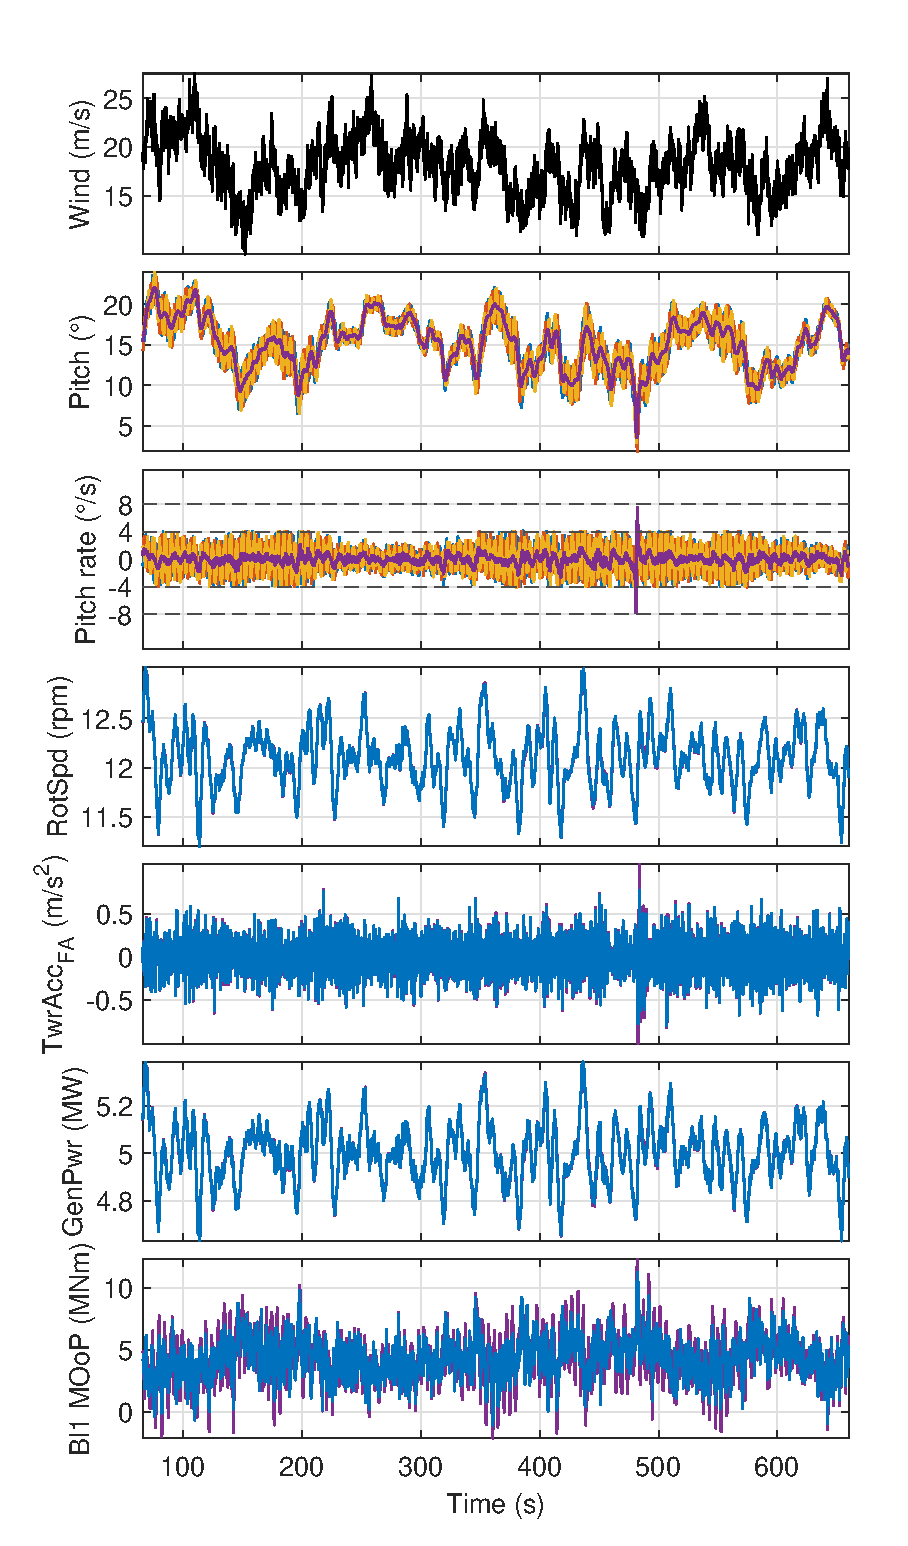
\includegraphics[width=0.495\textwidth,trim={0.cm 0cm 0cm 0.55cm}, clip]{figures/figIPCThesis/fig00a_Timeseries1.eps}}\hfill
    \subfloat[Pitch rate limit 13\textdegree/s, $K_{\text{P,IPC}}= 1.223$, $K_{\text{I,IPC}}= 0.365$]{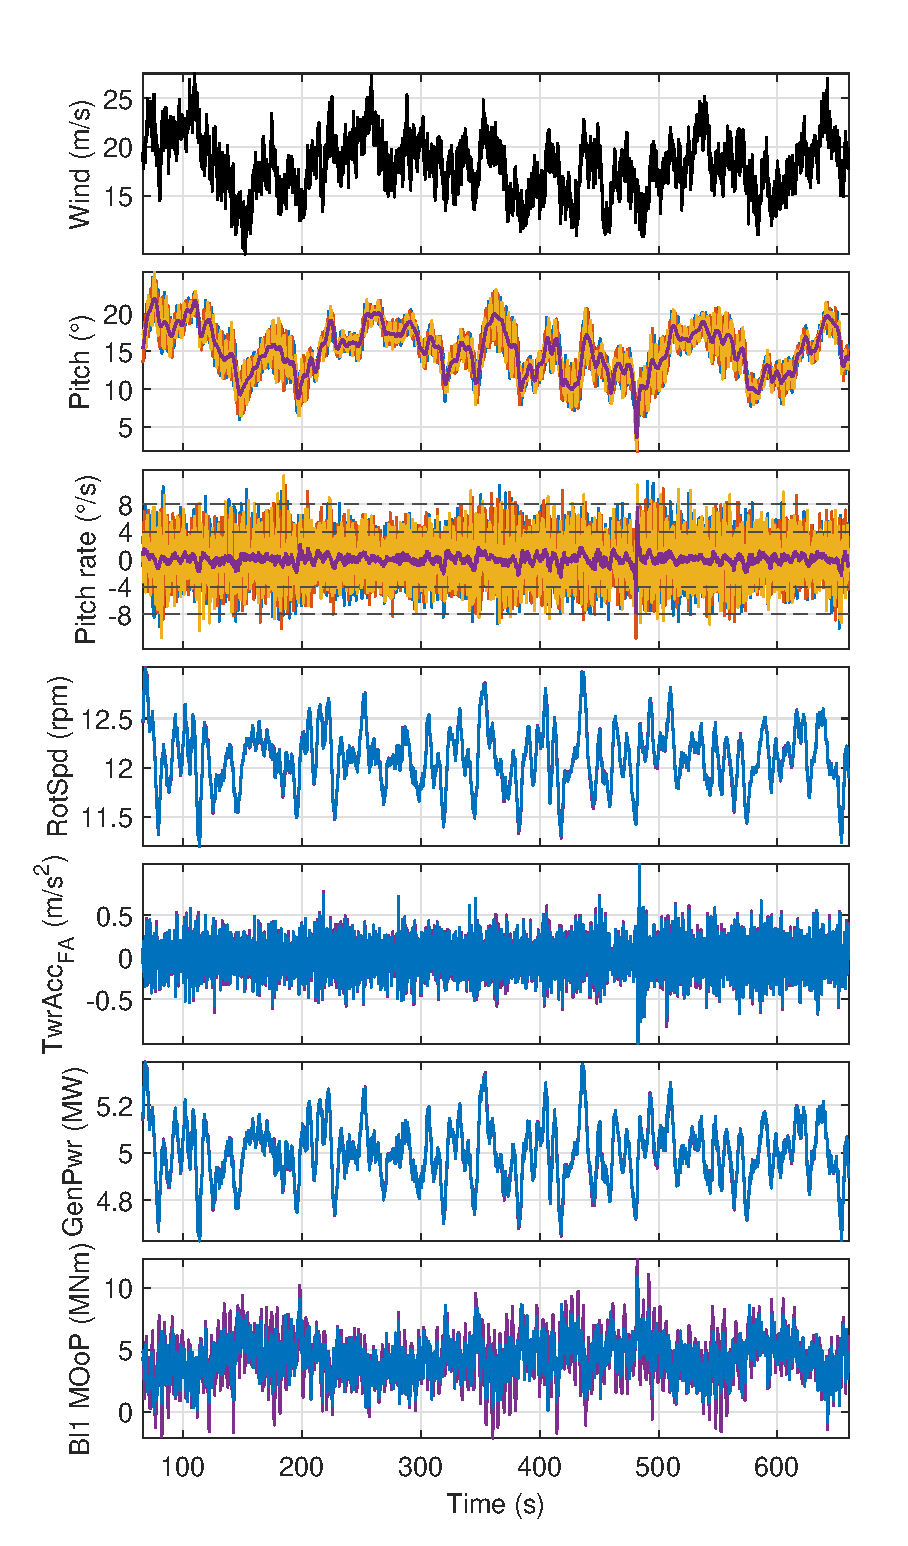
\includegraphics[width=0.495\textwidth,trim={0.cm 0cm 0cm 0.55cm}, clip]{figures/figIPCThesis/fig00a_Timeseries3.eps}}\hfill
    \caption[Controller comparison baseline CPC and IPC PI with different pitch rate limits.]{Controller comparison baseline CPC (\mlPurple) and IPC PI (\mlBlue, \mlOrange{} and \mlYellow{} pitch signals of blades 1 to 3, \mlBlue{} all other signals) with different pitch rate limits for turbulent wind (18\,m/s mean, turbulence class A, optimization dataset). Rate limits: Low (4\textdegree/s) and high (13\textdegree/s) for IPC, standard  (8\textdegree/s) for CPC PI. Dashed lines in the pitch rate plots: $\pm 4$\textdegree/s and $\pm 8$\textdegree/s. Displayed signals: freestream wind speed, pitch, pitch rate, states, power, and blade~1 root out-of-plane moment.}
    \label{fig:timeseriesIPC}
\end{figure}
%

%
Figure~\ref{fig:PSDIPC} shows the PSD of the blade root out-of-plane moment to visualize and explain the gradual improvement with increasing pitch rate for all three test cases. The black line represents the baseline CPC. The values given are the maxima of the PSD within 15\% of 1P and 2P. They represent the worst case in the vicinity of the rotor harmonics, which includes the spreading of the peaks due to the rotor speed variation and neighboring resonances. With IPC, the 1P peak is suppressed, so the value given is the largest PSD value in the 1P band rather than a distinct peak. The blue line, representing IPC with a 4\textdegree/s rate limit, reduces the 1P PSD peak by 91\%, while the orange line, representing IPC with an 8\textdegree/s rate limit, further lowers it, achieving a 96\% reduction. At the 2P frequency, the blue line shows only a small decrease of 11\% compared to the baseline, while the orange line lowers the 2P peak by 44\%. As expected, the 8\textdegree/s rate limit offers better load reduction across both 1P and 2P frequencies. The controller tuned with the rate limit set to 13\textdegree/s, depicted as a yellow dotted line, lies almost on top of the orange line, with 1P and 2P peak reductions of 96\% and 45\%, respectively.
\begin{figure}[h]
    \begin{center}
        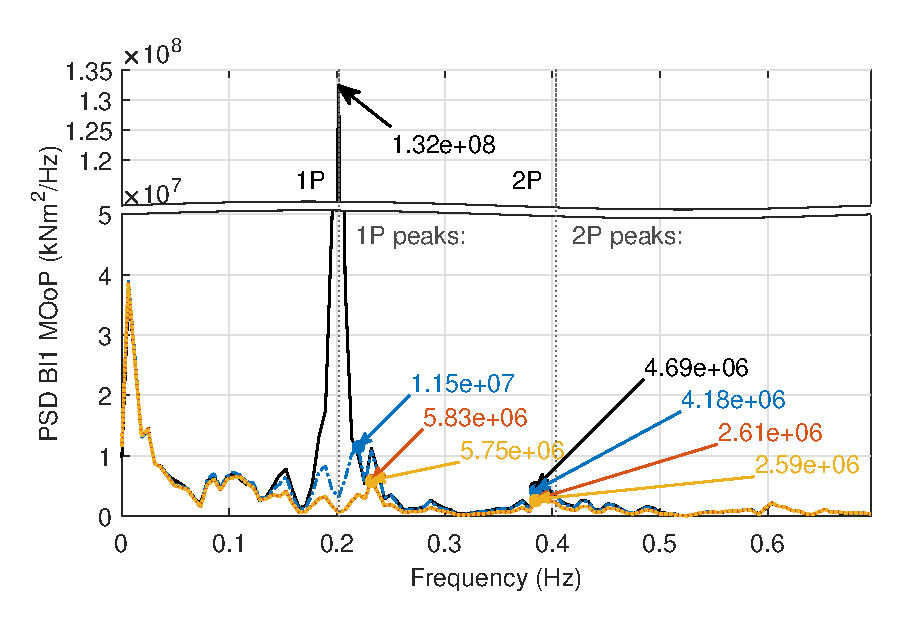
\includegraphics[width=0.6\textwidth]{figures/figIPCThesis/fig02_PSDroot_breaky_ratecomp.eps}
        \caption[Controller comparison: Power spectral density of the blade~1 root out-of-plane moment of baseline PI with 8\textdegree/s rate limit, IPC with 4\textdegree/s, 8\textdegree/s, and 13\textdegree/s rate limits]{Controller comparison: Power Spectral Density of the blade~1 root out-of-plane moment of baseline PI (\mBlack) with 8\textdegree/s rate limit, IPC with 4\textdegree/s rate limit (\mlBlueDashDot), 8\textdegree/s rate limit (\mlOrange), and 13\textdegree/s rate limit (\mlYellowDotted).}
        \label{fig:PSDIPC}
    \end{center}
\end{figure}
%
Table~\ref{tab:stddev_unified_IPC} summarizes the standard deviation of the signals shown in Figure~\ref{fig:timeseriesIPC} for IPC rate limits of 4\textdegree/s, 8\textdegree/s, and 13\textdegree/s. For all three cases, the baseline is the PI CPC with the standard rate limit of 8\textdegree/s. For the rotor speed and the power output, the introduction of IPC does not produce any observable effect, with ratios between 0.99 and 1.00. The tower fore-aft acceleration, whose differences are hardly visible in the time series, decreases slightly by 2\% to 3\%. The pitch rate standard deviation increases unavoidably for the IPC test cases: by a factor of 2.81 at the most restrictive limit of 4\textdegree/s, and by factors of 4.58 and 4.61 at 8\textdegree/s and 13\textdegree/s, respectively. In contrast, the blade root out-of-plane moment is reduced by 18\%, 25\%, and 25\% across the three limits, consistent with the spectral load reductions at 1P and 2P visible in Figure~\ref{fig:PSDIPC}.
\begin{table}[htbp]
    \centering
    \caption[Standard deviation of tower fore-aft acceleration, generated power, rotor speed, IPC blade pitch rate and blade root
    out-of-plane moment for turbulent wind.]{Standard deviation of tower fore-aft acceleration, generated power, rotor speed, IPC blade pitch rate and blade root
        out-of-plane (OoP) moment for turbulent wind (18\,m/s mean, turbulence class A) with different pitch rate limits, evaluated from 66\,s. Values in brackets show
        the ratio IPC/PI baseline (values below 1 indicate an improvement), with the PI baseline at the standard rate limit of 8\textdegree/s, whose standard deviations are 0.21\,m/s$^2$, 123.82\,kW, 0.30\,rpm, 0.65\textdegree/s, and 1986.63\,kNm, respectively.}
    \label{tab:stddev_unified_IPC}
    \begin{tabular}{l rrr}
        \toprule
        & \multicolumn{3}{c}{IPC rate limit (\textdegree/s)} \\
        \cmidrule(lr){2-4}
        Signal & low: 4 & standard: 8 & high: 13 \\
        \midrule
        Tower fore-aft acc.\ (m/s$^2$)  & 0.20 (0.98) & 0.20 (0.97) & 0.20 (0.98) \\
        Generated power (kW)             & 124.19 (1.00) & 123.30 (1.00) & 123.12 (0.99) \\
        Rotor speed (rpm)                & 0.30 (1.00) & 0.30 (1.00) & 0.30 (0.99) \\
        Blade pitch rate (\textdegree/s) & 1.83 (2.81) & 2.98 (4.58) & 3.00 (4.61) \\
        Blade 1 root OoP moment (kNm)    & 1624.02 (0.82) & 1483.35 (0.75) & 1481.16 (0.75) \\
        \bottomrule
    \end{tabular}
\end{table}
%
The IPC gains are optimized with a single wind field at 18\,m/s. To check whether they carry over to the whole of Region~III and to other wind fields, the IPC with the gains for 8\textdegree/s is simulated for all above rated wind speeds of the optimization dataset and of the two verification datasets, which are also used for the AALC in Section~\ref{subsec:ResultsTEF}. Table~\ref{tab:IPC_summary} contains the six evaluation criteria, normalized by simulations without IPC for the same wind test cases and averaged over three wind speed ranges: all wind speeds above rated, the wind speeds from 18\,m/s, and the optimization wind speed of 18\,m/s. As defined in Section~\ref{subsection: IPCOptCriteria}, the DELs are calculated with the W\"ohler exponents of 10 for the blades, summed over the three blades, and 4 for the tower, and all criteria are evaluated from 60\,s onward.
%
% Created by makeIPC_SummaryTable on 2026-10-26
\begin{table}[h]
    \centering
    \caption[Evaluation criteria for IPC: Mean values of the optimization and verification datasets over above-rated wind speed ranges]{\label{tab:IPC_summary} Evaluation criteria for IPC: Mean values of the optimization and verification datasets over above-rated wind speed ranges, normalized by the baseline PI without IPC; values below 1 indicate a reduction. IPC gains optimized at 18\,m/s with the pitch rate limit 8\textdegree/s: $K_{\text{P,IPC}} = 1.222$ and $K_{\text{I,IPC}} = 0.370$. Criteria are blade, tower
        base and tower top DELs, power mean and standard deviation, and pitch actuator power. The first verification set has no wind field for 13\,m/s.}
    
    %{ Evaluation criteria for IPC: Mean values of the optimization and verification datasets over the above rated wind speed ranges, normalized by the baseline without IPC. IPC gains optimized at 18\,m/s with the pitch rate limit 8\textdegree/s for all wind speeds: $K_{\text{P,IPC}} = 1.222$ and $K_{\text{I,IPC}} = 0.370$. Criteria are blade (sum of the three blades, W\"ohler exponent 10), tower base and tower top DELs (W\"ohler exponent 4, all evaluated from 60\,s), power mean and standard deviation (mean of the ratios of the single wind speeds), and actuator power (ratio of the mean actuator powers). The first verification set has no wind field for 13\,m/s.}
    \begin{tabular}{@{}l*{8}{c}@{}}
        \toprule
        Wind speeds & Dataset & Turb. class & $C_{\text{DEL},b}$ & $C_{\text{DEL},t,\text{Base}}$ & $C_{\text{DEL},t,\text{Top}}$ & $C_{\bar{P}}$ & $C_{\delta P}$ & $C_{\text{Act}}$ \\
        \midrule
        \multirow{3}{*}{\begin{tabular}[c]{@{}l@{}}Above rated\\(12--25\,m/s)\end{tabular}} & Optim. & A & 0.77 & 1.00 & 0.93 & 1.00 & 1.02 & 5.37 \\
        & Verif. 1 & A & 0.78 & 1.00 & 0.93 & 1.00 & 1.02 & 5.66 \\
        & Verif. 2 & B & 0.79 & 1.01 & 0.93 & 1.00 & 1.01 & 5.44 \\
        \midrule
        \multirow{3}{*}{18--25\,m/s} & Optim. & A & 0.75 & 1.01 & 0.94 & 1.00 & 1.01 & 5.84 \\
        & Verif. 1 & A & 0.76 & 1.01 & 0.95 & 1.00 & 1.01 & 5.97 \\
        & Verif. 2 & B & 0.75 & 1.02 & 0.93 & 1.00 & 1.01 & 5.89 \\
        \midrule
        \multirow{3}{*}{18\,m/s} & Optim. & A & 0.80 & 1.00 & 0.90 & 1.00 & 1.00 & 5.04 \\
        & Verif. 1 & A & 0.79 & 1.00 & 0.92 & 1.00 & 1.00 & 5.01 \\
        & Verif. 2 & B & 0.80 & 1.06 & 0.91 & 1.00 & 1.00 & 5.01 \\
        \bottomrule
    \end{tabular}
\end{table}


Above rated, the blade DEL decreases by 21\% to 23\%, and from 18\,m/s on by 24\% to 25\%, for all three datasets. The reduction grows with the wind speed: for the second verification set of turbulence class~B, it increases from 11\% to 16\% between 12 and 16\,m/s to 25\% to 27\% from 20\,m/s on. The gains optimized at a single wind speed hence carry over to the whole of Region~III and to both verification sets, so that no gain scheduling is required above rated. The tower base DEL is not changed considerably, with criteria between 1.00 and 1.01; the largest increase of a single wind speed is 6\% at 18\,m/s for turbulence class~B. The tower top DEL is reduced by about 7\% above rated and by 8\% to 10\% at 18\,m/s. Close to rated wind speed, the mean power decreases by up to 0.6\% and its standard deviation increases slightly, so that the power criteria above rated are 1.00 and 1.01 to 1.02. The pitch rate reaches the limit of 8\textdegree/s at all wind speeds, and the actuator power is increased by a factor of 5.4 to 5.7 above rated and of 5.8 to 6.0 from 18\,m/s on. Compared with the AALC (Table~\ref{tabone}), the IPC achieves about the same blade DEL reduction above rated (AALC: 22\% to 24\%), but at a clearly higher actuator power (AALC: factor 3.9 to 4.0); from 18\,m/s on, the AALC reduces the blade DEL slightly more (26\% to 27\%).


IPC was shown in this section to reduce blade loads, with the amount of reduction progressively increasing with higher pitch rate limits, at the cost of increased actuator energy. It was also shown to decrease tower loads to a certain degree. The IPC gains optimized at a single wind speed of 18\,m/s carry over to the whole of Region~III and to both verification datasets, with blade DEL reductions of 21\% to 23\% above rated at unchanged tower base DEL and power, but with an actuator power increased by a factor of 5.4 to 5.7. 
On the qLPV model without model mismatch, the qLMPC discussed in the previous section reduces the tower loads more effectively than IPC, as it directly controls the collective pitch to lower thrust fluctuations. On FAST, however, the adapted qLMPC designs increase the tower loads and do not reduce the blade loads, while IPC reduces the blade DEL without wind information. The performance of IPC also depends on the quality of the blade root out-of-plane moment measurements. Nevertheless, IPC PI controllers are currently more widely accepted as a relatively simple method for reducing blade loads on large turbines. A combination of qLMPC and IPC is investigated in Section~\ref{subsec:ComparisonWindTurbineControlDesigns}.

While this section focused on load mitigation through individual pitch control, further 
improvements can be achieved by including additional actuators. As blade sizes continue to 
increase, additional actuation devices integrated into the blade structure might become 
necessary. The following section introduces a turbine model enhanced 
with trailing edge flaps on the rotor blades, enabling combined IPC and flap control for 
more effective high-frequency load reduction.

\let\oldsectionmark\sectionmark
\renewcommand{\sectionmark}[1]{\oldsectionmark{Combined IPC-TEFC Design and Application}}
\section{Combined IPC and Trailing Edge Flap Control Design and Application}
\label{sec:CombinedIPC-TrailingEdgeFlapControl}
\let\sectionmark\oldsectionmark

Building on the previous investigations into IPC and qLMPC strategies, this section focuses on a combined control approach that incorporates both IPC and TEFs. By including TEFs in the rotor blades as supplementary actuation surfaces, additional degrees of freedom become available for targeted load mitigation, particularly at higher frequencies. This combination of individual pitch and trailing edge flap control is referred to as IPC-TEFC or AALC. AALC is defined as the integrated use of multiple aerodynamic actuators to actively reduce structural loads while preserving power output. By coordinating both individual blade pitch adjustments and trailing edge flap deflections, AALC can provide enhanced load mitigation compared to each method alone. This section presents the model formulation for incorporating TEFs into the wind turbine dynamics and evaluates a combined IPC-TEFC strategy across Regions~II and~III. The controller design is based on an optimization framework that considers multiple wind conditions and turbulence intensities to ensure good performance over the whole operating range. Several DLR studies have addressed TEFC optimization. In \cite{kumar2019load}, a first proof of concept is implemented. The TEFC scheme from that work is fine-tuned in \cite{adolph2022reglerparameteroptimierung}. In \cite{osterwinter2023load}, the parameters of a combined IPC-TEFC approach are optimized and validated using a comprehensive set of verification wind fields to assess load reduction, power preservation, and actuator demand. Results from this report are published in \cite{dittmer2024combined}.


\subsection{TEF Simulation Model} %bonnie_jonkman_openfastopenfast_2022 OpenFAST2023
As before, the OpenFAST simulation software is used to investigate the benefits of combining individual pitch and trailing edge flap control. The NREL 5MW wind turbine model is modified to implement controllable trailing edge flaps on the rotor blades. The original NREL 5MW model without TEF serves as a reference for analyzing the aerodynamic effects of these modifications on the simulated operation of the turbine. 
\subsubsection*{Rotor Blade Geometry and Aerodynamics}
The rotor blades of the NREL 5MW turbine are defined by eight distinct cross-sectional profiles distributed along the blade length, as illustrated in Figure~\ref{subfig:TEF1}, and comprise 19 nodes, each with specific geometric profile shapes. At the root, cylindrical profiles connect to the rotor hub, accommodating high bending moments and pitch adjustments. The profiles transition from the DU series, developed at Delft University of Technology, near the root to the NACA64 profile in the outer 29\% of the blade, characterized by decreasing thickness towards the tip. The blade's aerodynamic efficiency is further refined by varying the profile depth and orientation at each node.

The blade section with trailing edge flaps, which covers the whole NACA64 blade section, is marked in red. The flap-to-blade chord ratio amounts to 20\%. The aerodynamic model of the blade enhanced with TEF requires input data on lift, drag, and pitching moment coefficients for all profiles across various blade angles of attack and a variety of flap deflection angles. The three main factors influencing these aerodynamic properties are surface roughness, Mach number, and Reynolds number. The OpenFAST simulation neglects surface roughness variations due to contaminants. The airflow is assumed to be incompressible with a Mach number of 0.25 at the blade tip. OpenFAST can interpolate between polars based on either the Reynolds number or a user-defined parameter. In this work, the user-defined parameter is the flap angle, i.e., the interpolation is performed between the polars of the different flap angles. As only one interpolation parameter can be defined, the Reynolds number distribution depicted in Figure~\ref{subfig:TEF1} is used for all wind speeds. Reynolds numbers ranging from one to eight million are obtained from an OpenFAST simulation with turbulence class A at a mean wind speed of 12\,m/s. Care was taken to model the distribution of Reynolds numbers along the rotor blade at this wind speed as realistically as possible. The OpenFAST aerodynamic models of the rotor blades are extended with additional airfoil polars based on this distribution.  % with the numbers obtained via an OpenFAST simulation run with a wind file from the optimization dataset, with turbulence class A and the meand wind speed at 12\,m/s.
\begin{figure}[h]
    \centering
    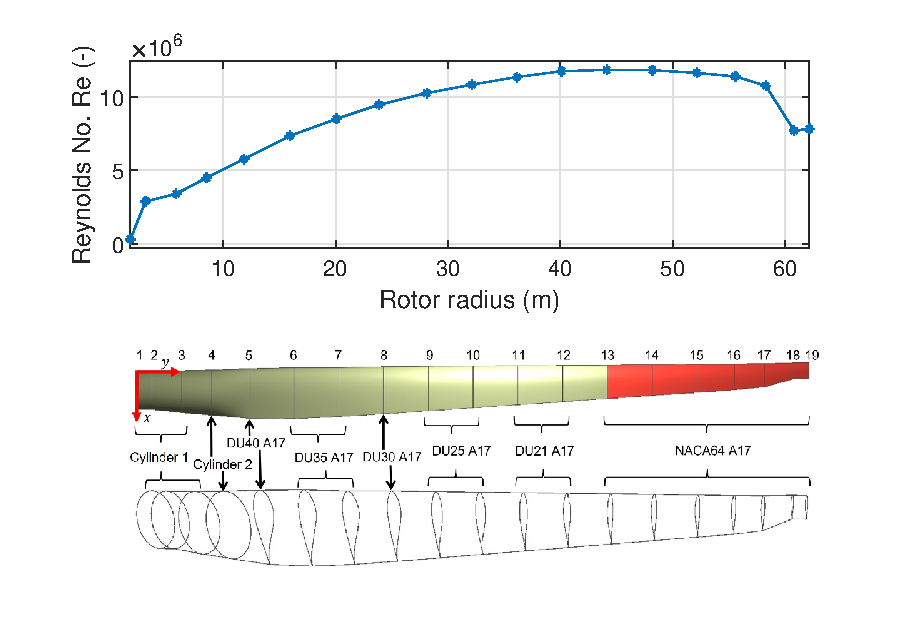
\includegraphics[width=0.6\textwidth]{figures/Images_Torque24/fig01_RE.eps}\hspace{0pc}%
    \begin{minipage}[b]{0.95\textwidth}\caption[ Span-wise distribution of Reynolds numbers Re at wind speed $V_{\infty} = 12$\,m/s]{\label{subfig:TEF1} Span-wise distribution of Reynolds numbers Re at wind speed $V_{\infty} = 12$\,m/s (from OpenFAST simulation) and blade geometry with cylinder, DU40, DU35, DU30, DU25, DU21 and NACA64 profiles with TEF location covering the NACA64 section marked in red.}
    \end{minipage}
\end{figure}

\subsubsection{Polar Calculation with xflr5 and XFOIL}
The aerodynamic coefficients of rotor blade profiles for the TEF-enhanced blades are calculated using the programs xflr5 and XFOIL, see \cite{drela1989xfoil}. XFOIL uses a higher-order panel method to analyze and design airfoil profiles, incorporating variables like Reynolds number, Mach number, and a transition criterion for calculating the shift from laminar to turbulent flow. The turbulence degree of the incoming flow determines the appropriate transition criterion value, with the default value set at 9, approximating a median turbulence level as per XFOIL's documentation. For fluid properties, standard sea-level values from the International Standard Atmosphere (ISA) are used. The aerodynamic coefficients for the respective profiles are calculated based on the Reynolds numbers selected from Figure \ref{subfig:TEF1}. The coefficients generated by xflr5 and XFOIL are not directly suitable for wind turbine simulation as AeroDyn15 requires coefficients over an angle of attack range from -180\textdegree{} to +180\textdegree. Since XFOIL's panel methods yield accurate results only up to the point of flow separation, the polars are extrapolated to cover the entire required angle range. This extrapolation is performed using the AirfoilPrep preprocessor developed by NREL, applying the Viterna method for extrapolating polars, see for details e.g.~\cite{gasch2011wind}. %on Viterna's calculation process 
Additionally, corrections are made to account for three-dimensional flow effects caused by the rotor blade's rotation. Factors like Coriolis and centrifugal forces increase the maximum lift coefficients in the inner rotor areas. These 3D effects are corrected using functions integrated into AirfoilPrep. Figure \ref{subfig:TEF2} illustrates the extrapolated and corrected lift and drag coefficients over the angle of attack for rotor blade profiles with different flap angles. 

Figure~\ref{subfig:TEF2}\,(a) shows that a positive flap deflection increases the lift coefficient $c_l$ and hence the lift. A positive flap deflection $\eta_{\text{TEF}}$ is defined as the trailing edge of the flap moving towards the pressure side, relative to the chord line of the local blade profile with undeflected flap. The maximum lift coefficient occurs at a smaller angle of attack than with a neutral flap position. A negative flap deflection has the opposite effect: the lift coefficients are reduced and the maximum lift coefficient shifts to higher angles of attack. This corresponds to the expected effect of trailing edge flap deflections on the lift. 
%
\begin{figure} [htbp]
    \centering
    \subfloat[Lift coefficient $c_{l}$]{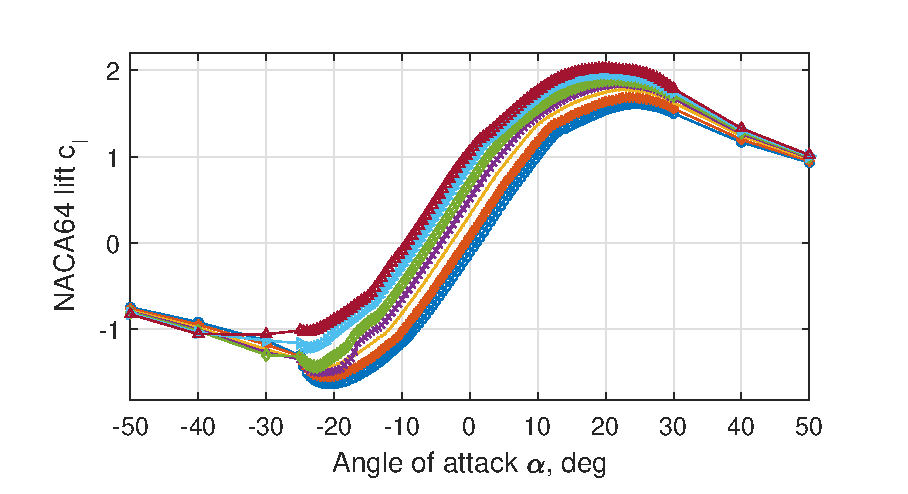
\includegraphics[width=0.495\textwidth,trim={0.cm 0cm 0cm 0.5cm}, clip]{figures/Images_Torque24/fig01_Cl1out.eps}}\hfill 
    \subfloat[Drag coefficient $c_{d}$]{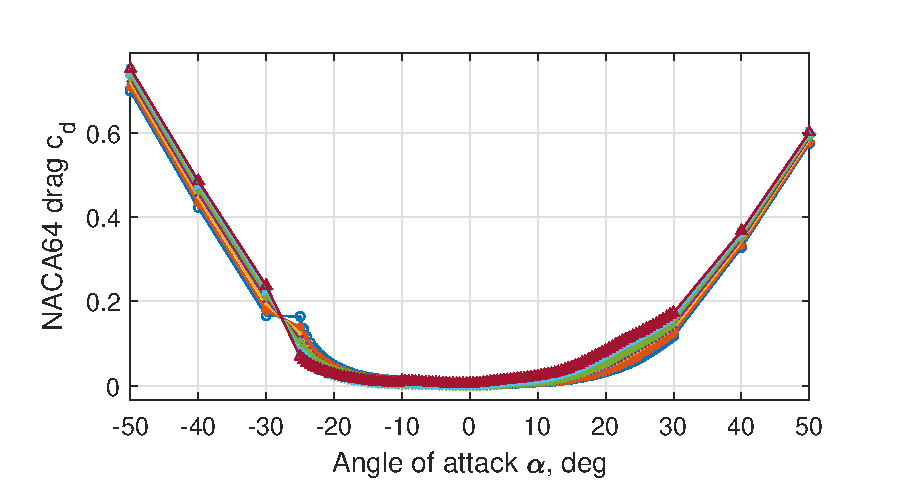
\includegraphics[width=0.495\textwidth,trim={0.cm 0cm 0cm 0.5cm}, clip]{figures/Images_Torque24/fig01_Cd1out.eps}}   
    \caption[Lift and drag coefficients at different trailing edge flap angles $\eta_{\text{TEF}}$ and blade angles of attack $\alpha$]{Lift and drag coefficients over the blade angle of attack $\alpha$ for the trailing edge flap angles $\eta_{\text{TEF}} = -10^\circ$ (\mlBlueCircle), $-7^\circ$ (\mlOrangeStar), $-3^\circ$ (\mlYellowLine), $0^\circ$ (\mlPurpleCross), $3^\circ$ (\mlGreenDiamond), $7^\circ$ (\mlCyanTriangle), and $10^\circ$ (\mlMaroonTriangle). The data are physically plausible for $-27^\circ \le \alpha \le 30^\circ$.}
    \label{subfig:TEF2}
\end{figure}
Figure~\ref{subfig:TEF2}\,(b) shows the drag coefficient. The curves of the drag coefficient $c_d$ are smooth and physically plausible for angles of attack above $-27^\circ$. Below this value, the vertical order of the polars suddenly reverses. There is no physical explanation for this effect, and no such discontinuity occurs for the rotor profile without trailing edge flap. Presumably, the extrapolation method does not work well for flapped profiles at these large negative angles of attack, where flow separation and stall occur. However, this can be disregarded, as the angles of attack in the outer region of the rotor blades do not fall below $-27^\circ$ during normal operation. As this study uses OpenFAST v3.2.1, no additional code is needed to include the TEF, unlike earlier studies based on previous FAST versions. The obtained coefficients are stored in an airfoil file, which is referenced in the Airfoil Information section of the AeroDyn15.dat file of the NREL 5MW model available in the Git repository~\cite{GitRepoCodeAALC}. %NACA64_A17_Flap.dat

%
\subsubsection*{Baseline Power Controller} %speed-controlled-pitch-controlled
In order to realistically simulate a modern turbine, a control system controlling rotor speed and generator torque is required, and the same baseline controller described and applied in the previous sections is utilized for that purpose. The aim of the IPC-TEFC is to further decrease the mechanical loads. Note that this load reduction controller using IPC together with TEF control is an add-on controller to the baseline control system. This is possible as cyclic pitch motions are induced, which are effectively decoupled from the collective pitch motion, ensuring rated power output above rated wind speed. As before, the implementation of the baseline controller is the power controller available within TU Delft's FASTTool, see \cite{mulders2020wind}. 
%
\subsubsection*{Open-Loop TEF Model Verification with FAST} % with TEF open loop control
The modified NREL 5MW turbine model presented in the previous section is tested in open-loop simulations with regard to the plausibility of the influence of the TEF position on the simulation results. The aerodynamic model of the trailing edge flap is included. Open-loop control inputs of the TEF deflection angle $\eta_{\text{ref}}$ are analyzed in order to investigate its suitability with regard to the desired DEL reduction. The effects of flap deflections on different parameters relevant to the operational quality of the wind turbine, such as forces and moments as well as power yield, are investigated. Figure \ref{fig:OLdiag} shows a block diagram to illustrate the control structure used for these verification tests, with the eight inputs, i.e., the seven control inputs and the wind of the selected test case $V_{\text{TC}}$ as a disturbance. The actuators for the pitch angle adjustment of the rotor blades are modeled as a first-order transfer function with position and rate limitations. The influences of different TEF positions for steady-state operating conditions are discussed in Section~\ref{subsec:ResultsTEF}. 
% For a sensitivity study of the flaps with regard to their influence on the blade root flapping moments, we refer to \cite{osterwinter2019load1}.
\begin{figure}[h]
    \centering
    \includegraphics[width=0.95\textwidth, trim=0 0 0 13, clip]{figures/Images_Torque24/blockdiagram_OL_latex_tau2.pdf}\hspace{2pc}%
    \begin{minipage}[b]{0.95\textwidth}
        \caption[Block diagram for open-loop TEF verification tests.]{\label{fig:OLdiag} Block diagram for open-loop TEF verification tests: the power control, consisting of the gain-scheduled PI pitch control and the $k\omega_g^2$ torque control, operates in closed loop on the generator speed $\omega_g$, while all three flaps receive the same constant reference $\eta_{\text{ref}}$ in open loop. The wind $V_{\text{TC}}$ of the respective test case acts as a disturbance.}    
        
        
        %\caption{\label{fig:OLdiag} Block diagram for open-loop TEF verification tests with baseline power control in closed loop and open-loop collective TEF control inputs.}
    \end{minipage} %BlockschaltbildopenLoop1.jpg
\end{figure}

%\caption[Block diagram for open-loop TEF verification tests]{\label{fig:OLdiag} Block diagram for open-loop TEF verification tests: the baseline power control, consisting of the gain-scheduled PI pitch control and the $k\omega_g^2$ torque control, operates in closed loop on the generator speed $\omega_g$, while all three flaps receive the same constant reference $\eta_{\text{ref}}$ in open loop. The wind $V_{\text{TC}}$ of the respective test case acts as a disturbance.}

\subsection{IPC-TEFC Implementation}
The main design objective of the presented AALC is the reduction of structural moments, focusing on the out-of-plane blade root bending moments. The overall controller layout is shown in Figure~\ref{fig:CLdiag}. The baseline controller, depicted in Figure~\ref{fig:OLdiag}, is enhanced with IPC, with the individual pitch demand added to the collective pitch reference, as well as TEFC which changes the TEF position. All six AALC control output signals are calculated via MBC, see Section \ref{sec:MBC}, based on the three out-of-plane blade root moments, $M_{yc1}$, $M_{yc2}$, and $M_{yc3}$, as well as the rotor azimuth $\theta_r$. This section reviews the allocation of IPC and TEFC signals and then discusses the design of these controllers. 
\begin{figure}[h]
    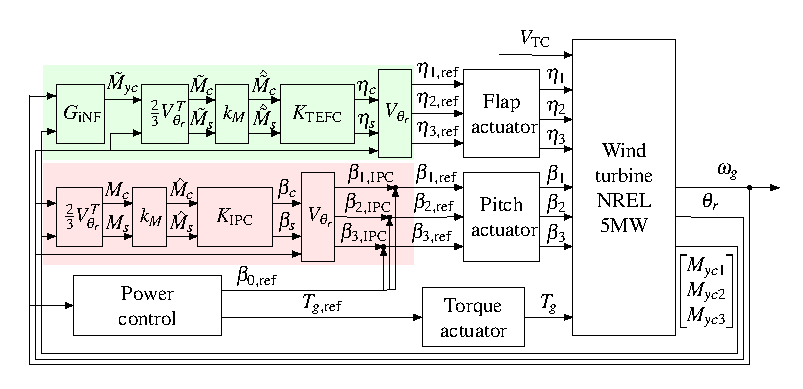
\includegraphics[width=0.95\textwidth]{figures/Images_Torque24/blockdiagram_CL_latex2.pdf}\hspace{2pc}%
    \begin{minipage}[b]{0.95\textwidth}  
        \caption[Block diagram of the closed-loop AALC with baseline power control, IPC, and TEFC]{\label{fig:CLdiag} Block diagram of the closed-loop AALC: the power control sets the collective pitch and generator torque references. The IPC (red) transforms the blade root moments $M_{yci}$ via MBC into the tilt and yaw moments, whose controller outputs are transformed back into individual pitch demands added to $\beta_{0,\text{ref}}$. The TEFC (green) has the same structure, but the inverse notch filter $G_{\text{iNF}}$ emphasizes the 2P loads, and the outputs are the flap references $\eta_{i,\text{ref}}$.}
        
    \end{minipage}
\end{figure}

%

%       \caption[Block diagram for closed-loop TEF verification tests with baseline power control, individual pitch and TEF closed loop control.]{\label{fig:CLdiag} Block diagram for closed-loop verification tests with baseline power control, individual pitch (highlighted in red) and TEF (highlighted in green) closed loop control.}

\subsubsection*{IPC and TEFC Control Allocation}
As for the IPC, the rotating blade root out-of-plane moments are transformed into the fixed coordinate system via MBC, see Section~\ref{sec:MBC} and Equation~\eqref{eq:MBC}.

Figure~\ref{fig:CLdiag} denotes $M_{yci}$ as the out-of-plane blade root moment of the $i$-th blade as inputs, and the rotor tilt moment $M_c$ and yaw moment $M_s$ in the non-rotating system as outputs. The moments $M_c$ and $M_s$ are used to calculate two cyclic control signals $q_c$ and $q_s$, i.e., $\beta_c$ and $\beta_s$ for IPC, and $\eta_c$ and $\eta_s$ for TEFC. The control signal $q_i$ of the $i$-th blade is calculated via the inverse MBC transformation in Equation~\eqref{eq:inverseMBC},
where the signal $q_i$ denotes $\beta_{i,\text{IPC}}$ and $\eta_{i,\text{ref}}$ in IPC and TEFC, for the $i$-th blade or flap, respectively. As for the IPC scheme, the tilt and yaw moments $M_c$ and $M_s$ are controlled via $q_c$ and $q_s$ independently, i.e., any remaining coupling following the MBC transformation between $q_c$ and $M_s$ as well as $q_s$ and $M_c$ is neglected. As the wind turbine dynamics can be approximated as an LTI system after transforming rotor blade dynamics into a fixed coordinate system, using MBC from Equation~\eqref{eq:MBC}, a simple, intuitive control approach is adopted. Four separate SISO controllers, two each for IPC and TEFC, are designed to reduce the transformed moments $M_c$ and $M_s$. The system is now over-actuated, i.e., two moments, $M_c$ and $M_s$, need to be mitigated, but four control inputs, $\eta_c$, $\eta_s$, $\beta_c$, and $\beta_s$, are available. This offers the possibility of a frequency separation as a form of control allocation. To achieve this frequency separation of IPC and TEFC, inverse notch filters are implemented in the AALC controller. The 1P loads in the frequency spectrum of the blade root bending moments are addressed with the IPC control loop. The 2P loads are addressed with the trailing edge flap controller making use of the fast flap dynamics. While modern MIMO controllers, e.g., AALC extension of the $H_\infty$ control \cite{ossmann2021field,ossmann2017load} or MPC \cite{dittmer2021velocity}, have the potential to optimize the available control inputs regarding the criteria listed in Section~\ref{sec:ControllerParameterOptimization} more efficiently, this simple, intuitive control allocation is selected as the resulting controller does not employ an observer-based structure and hence does not require the design of an explicit mathematical plant model.%via strategies such as MPC, LQG or $H_\infty$ control. %Details are elaborated below.

\subsubsection*{Individual Pitch Control for 1P Load Reduction}
The IPC controller $K_{\text{IPC}}$, illustrated in the red part of Figure \ref{fig:CLdiag}, receives the blade root out-of-plane moments $M_{yc1}$, $M_{yc2}$, and $M_{yc3}$ from the rotating coordinate systems, transforming them into fixed coordinate system moments $M_c$ and $M_s$ via MBC without additional filtering. This approach obviates the need for low-pass filtering within the IPC loops, as the actuator models already provide inherent low-pass filtering characteristics. The transformed moments are scaled with $k_M = 10^{-5}$, a value chosen due to the order-of-magnitude difference between the moments and the control angles in units of radians. The scaled moments $\hat{M}_s$ and $\hat{M}_c$ are passed to two identical SISO controllers. These controllers are based on the assumption that the transformed moments become largely independent after the transformation. The LTI nature of the transformed system allows for the potential use of PI controllers. Moreover, for IPC, which focuses on mitigating low-frequency load changes, particularly the 1P loads caused mainly by wind shear, a controller with an integral gain is first tuned manually. The integral component adequately addresses the control requirements by minimizing the steady-state error of the transformed moments and thus effectively targets the minimization of the 1P loads in the rotating coordinate system. This aids in decoupling the IPC from the TEFC controller, with the TEFC used for controlling higher frequencies. The calculated control signals $\beta_c$ and $\beta_s$ are converted back to the rotating blade coordinate systems via the inverse MBC given in Equation~\eqref{eq:inverseMBC}, resulting in the three signals $\beta_{i,\text{IPC}}$. The IPC exclusively calculates individual pitch angle components, avoiding interference with collective pitch angles calculated by the baseline power controller. The pitch angle commands, passed to the pitch actuators, $\beta_{i,\text{ref}}$ are calculated by adding the collective pitch angle command $\beta_{0,\text{ref}}$ to these individual pitch reference signals. The actuator model is implemented as a first-order transfer function with time constant $\tau_{\beta}=0.1$\,s with the angle limited from -2\textdegree{} to 90\textdegree{} and the rate limited from -8\textdegree{}/s to 8\textdegree{}/s. The pitch actuator angles $\beta_i$ are then applied to the OpenFAST NREL 5MW wind turbine model.

\subsubsection*{Trailing Edge Flap Control and Inverse Notch Filter for 2P Load Reduction}
The controller for the individual trailing edge flap control $K_{\text{TEFC}}$ is constructed similarly to the IPC: the MBC and inverse MBC enclose two identical SISO controllers for the transformed moments.

A key difference is that the blade root out-of-plane moment signals are filtered through an inverse notch filter before MBC processing, amplifying selected frequencies
\begin{equation*}
    G_{\text{iNF}}(s) = (s^2 +2k_{\text{iNF}}D\omega_{\text{iNF}}s +\omega_{\text{iNF}}^2)/ (s^2 +2D\omega_{\text{iNF}}s +\omega_{\text{iNF}}^2),\quad k_{\text{iNF}}=10,\quad D = 0.1
\end{equation*}
with the frequency $\omega_{\text{iNF}} = 2 \cdot 2\pi f_r$, i.e., twice the current rotor frequency $f_r$, and $s$ being the Laplace variable. This enhances 2P load amplitudes in the signals, enabling the TEFC to predominantly respond to these loads, thus minimizing mutual influence with the IPC. Post-filtering, the three blade root out-of-plane moments $\tilde{M}_{yci}$ are transformed into the fixed coordinate system via a multiplication with $2/3 V^T_{\theta_r}$, with the resulting moments $\tilde{M}_{c}$ and $\tilde{M}_{s}$. These are both scaled with $k_M$ to $\hat{\tilde{M}}_c$ and $\hat{\tilde{M}}_s$. Initially, two proportional controllers are used, with the manually tuned proportional parameter used as a starting point for the optimization of the controller parameters. The transformed control outputs are then converted back for flap angle adjustments, with flap actuators modeled for a more rapid response than the pitch actuators, aiding in 2P load reduction. The TEF actuator is modeled as a first-order transfer function with time constant $\tau_{\eta}=0.05$\,s, with the angle limited from -10\textdegree{} to 10\textdegree{}, and the rate limited from -20\textdegree{}/s to 20\textdegree{}/s.

\subsection{IPC-TEFC Parameter Optimization} \label{sec:ControllerParameterOptimization}
As for IPC, the AALC gains at 18\,m/s are optimized with \textit{fminsearch} followed by \textit{fmincon} with the tower constraint, for the pitch rate limit of 8\textdegree/s and with the fade-in of the IPC and TEF inputs. The procedure is as follows:
\begin{enumerate}
    \item A preliminary optimization of the proportional TEFC gain $K_{\text{P,TEFC}}$ is run with fixed IPC gains ($K_{\text{P,IPC}} = 0.62$, $K_{\text{I,IPC}} = 0.32$, from an IPC optimization before the fade-in was introduced). The integral and derivative gains of the TEFC, $K_{\text{I,TEFC}}$ and $K_{\text{D,TEFC}}$, are set to zero; a joint optimization of $K_{\text{D,TEFC}}$ resulted in a value close to zero ($K_{\text{D,TEFC}} = 0.002$) without a noticeable decrease of the cost. A TEF integral gain would shift the low-frequency control effort at 1P from the pitch to the flaps. It would lower the pitch activity but raise the flap activity, for a negligible blade DEL gain. It was therefore not used. For this optimization step, only \textit{fminsearch} is used to optimize the proportional gain, resulting in $K_{\text{P,TEFC}} = 0.24$.
    \item The proportional and integral gains of the IPC and the proportional gain of the TEFC are optimized jointly at 18\,m/s, starting from the IPC gains optimized for 8\textdegree/s ($K_{\text{P,IPC}} = 1.22$, $K_{\text{I,IPC}} = 0.37$) and $K_{\text{P,TEFC}} = 0.24$ from the preliminary optimization. In this step, \textit{fminsearch} is followed by \textit{fmincon}. As the result of \textit{fminsearch} already satisfies the tower constraint, \textit{fmincon} does not change it.
\end{enumerate}
Below rated, the three gains are optimized jointly for each of the wind speeds 4, 6 and 8\,m/s, with \textit{fminsearch} only, since the tower DEL decreases below rated anyway and the tower constraint is not needed. The optimization is started from the initial gains of \cite{dittmer2024combined}, i.e., a purely integral IPC and a purely proportional TEFC, each with a gain of one.


As for the IPC, the quality of an AALC controller is quantified via the decrease in blade root DEL. The cost function $J$ to be minimized by the AALC is the maximum of the DEL of the three blades, i.e., the same cost function as provided in Equation~\eqref{eq:costFunIPC}.
To evaluate and quantify the impact of an AALC controller's performance, the same criteria as before are used, which can be summarized as follows:

\begin{itemize}
    \item \textbf{Blade DEL $C_{\text{DEL},b}$ and tower DEL $C_{\text{DEL,t}}$:} Reducing the blade DEL is the main incentive for using
    IPC to decrease the PSD at 1P. Load reductions at the 1P frequency do
    not directly influence the tower base DEL, while decreasing the PSD at the 2P frequency via the
    flaps also decreases the tower top DEL. Therefore, a decrease in tower top DEL is observed although this criterion is not included in the objective function.  
    \item \textbf{Power mean $C_{\bar{P}}$ and standard deviation $C_{\delta P}$:} The power criteria were also not included in the
    optimization. As the annual energy production is typically not allowed to decrease from AALC,
    the generated power was compared for all test cases above rated and it was found
    that the power production loss and variance increase are negligible. % The power
    %variance is important for the stability in small networks. The effect of the AALC controller was found to be nearly negligible.
    \item \textbf{Actuator power $C_{\text{Act}}$:} This is the only criterion for which an increase is
    unavoidable, due to the additional movement of the blade that
    the IPC requires; the flap actuators are not included in this criterion. %With the activation of individual pitch control, the pitch actuator power tripled to approximately 4.5 kW for all pitch actuators.
\end{itemize}
As for the IPC, the optimization dataset with wind of turbulence class~A is used to optimize the parameters at 18\,m/s above rated and, in addition, at 4, 6, and 8\,m/s below rated. As before, the pitch rate limit is fixed at 8\textdegree/s. The AALC's effect is analyzed by incorporating five wind speeds in Region~II, from 4\,m/s to 11\,m/s, and nine wind speeds in Region~III, ranging from 12\,m/s to 25\,m/s. Two verification sets are created for the 14 wind speeds, with the wind fields for 11 and 13\,m/s missing in the first one: one with turbulence class~A using a different seed, and one with turbulence class~B. The vertical wind speed distribution is modeled with a power law wind profile to represent wind shear, using an exponent of 0.2. All wind fields are available in the Git repository \cite{GitRepoCodeAALC}, which also includes the code to reproduce all results presented here. 

\subsection{Results} \label{subsec:ResultsTEF}
This section discusses both open-loop results, obtained with the simulation setup depicted in Figure~\ref{fig:OLdiag}, and closed-loop results, simulated with the control loop from Figure~\ref{fig:CLdiag}. 

\subsubsection{Open-Loop Results}
Figure~\ref{fig:OLval} shows the steady-state values, at three different TEF angles, of power $P_g$, rotor speed $\omega_r$, rotor thrust $F_{T_r}$, and blade pitch angle $\beta_{0}$ for all 14 wind speeds. Simulations at constant wind speeds are run for 660\,s to confirm the plausibility of the TEF model. Data from the initial 60\,s are excluded to avoid non-physical initialization artifacts and the mean values are calculated for each wind speed.
\begin{figure} [htbp]\centering
    \centering
    % \subfloat[Power and rotor speed]{\includegraphics[width=0.65\textwidth]{figures/Images_Torque24/fig06_TEFOL_1.eps}}\\
    % \subfloat[Rotor thrust and blade pitch]{\includegraphics[width=0.65\textwidth]{figures/Images_Torque24/fig06_TEFOL_2.eps}}
    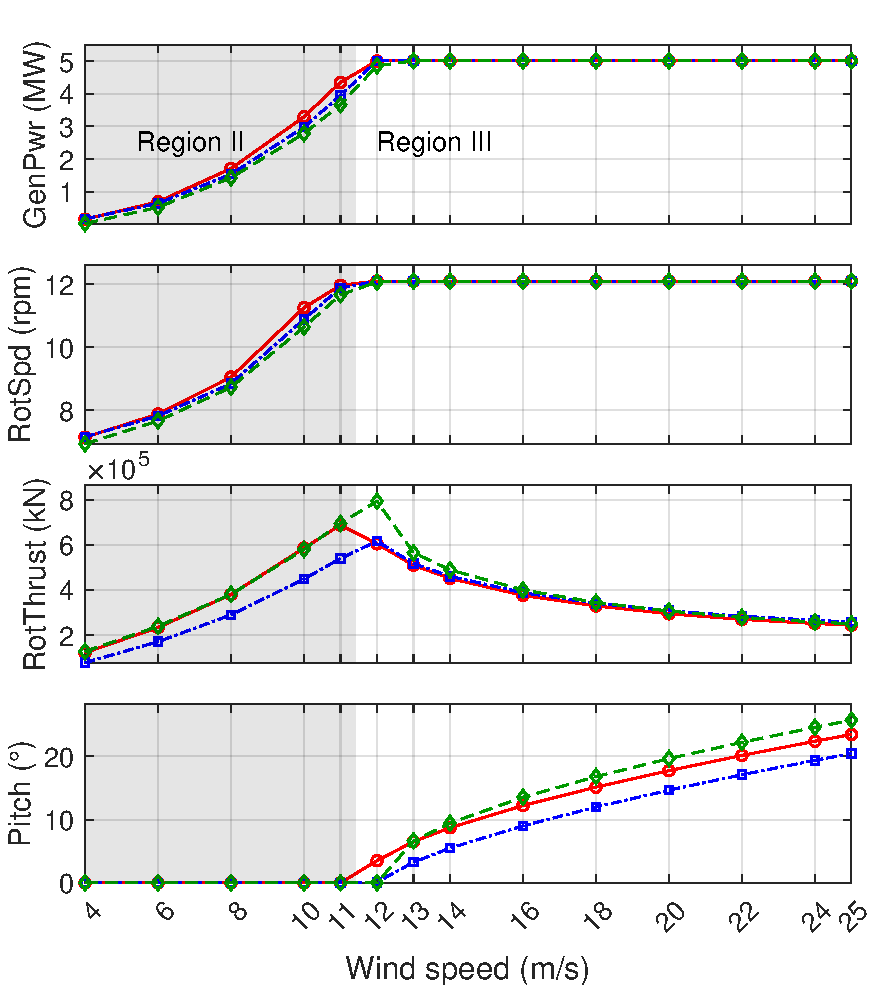
\includegraphics[width=0.6\textwidth]{figures/Images_Torque24/fig06_TEFOL.pdf}
    \caption[TEF open-loop verification: Mean values for TEF deflections of -10\textdegree{}, 0\textdegree{}, and 10\textdegree{} for constant wind.]{TEF open-loop verification: Mean values for TEF deflections of -10\textdegree{}\,(\mlBlueDashDotSquare), 0\textdegree{}\,(\mlRedCircle), and 10\textdegree{}\,(\mlDarkGreenDashedDiamond) for constant wind. Region~II and Region~III marked with gray and white backgrounds, respectively. Displayed signals: Power, rotor speed, rotor thrust, and blade pitch.}
    \label{fig:OLval}
\end{figure}

%
The simulated power with and without TEF deflections shows the expected power characteristic curve of a wind turbine: In Region~II, both positive and negative flap deflections reduce power \(P_g\) due to decreased aerodynamic efficiency, unlike in Region~III, where the same power output is observed, as the power controller controls the pitch angle once rated wind speed is reached. Adjusting the pitch changes the aerodynamic forces. The control system can therefore maintain nominal power. This is also reflected in the rotor speed \(\omega_r\), depicted in the second plot, which is slightly lower in Region~II but unchanged in Region~III. The thrust \(F_{T_r}\) in Region~II is decreased by a negative flap angle, while the influence of a positive flap angle on the thrust is negligible: The higher lift is offset by the lower rotor speed and hence lower relative inflow velocity. The fourth plot in Figure~\ref{fig:OLval} shows the blade pitch \(\beta_{0}\), which is lower for a negative and higher for a positive TEF angle, corresponding to the lower and higher thrust force.

\subsubsection{Closed-Loop Results}
Figure~\ref{fig:PSDTEF} shows the PSD of the blade root bending moment in closed loop for the optimization dataset with a mean wind speed of 18\,m/s, the wind speed at which the AALC parameters are optimized.
\begin{figure}[htbp]
    \centering
    \subfloat[Baseline (\mBlack), IPC (\mlOldBlue), and TEFC (\mlDarkGreen)]{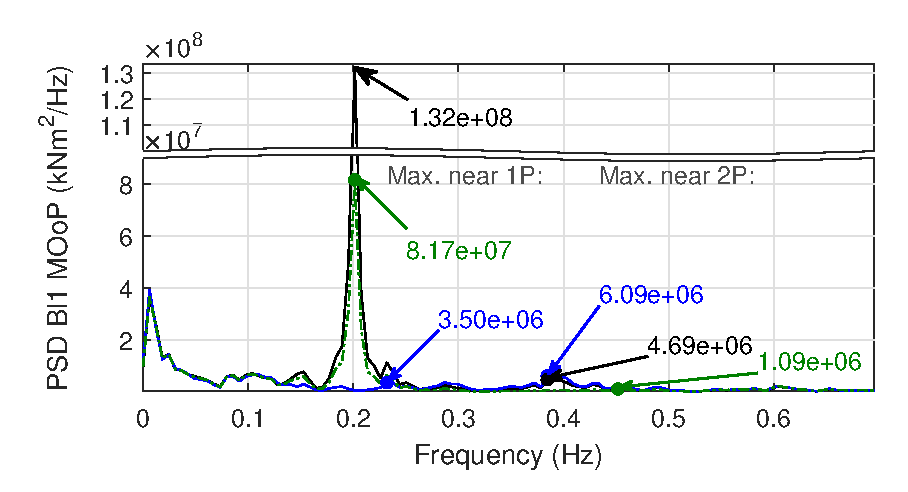
\includegraphics[width=0.65\textwidth]{figures/figIPCThesis/fig02_PSDroot_breaky_AALCinit.eps}}\\
    \subfloat[Baseline (\mBlack), AALC (\mlRed), and AALC optimized (\mlPink)]{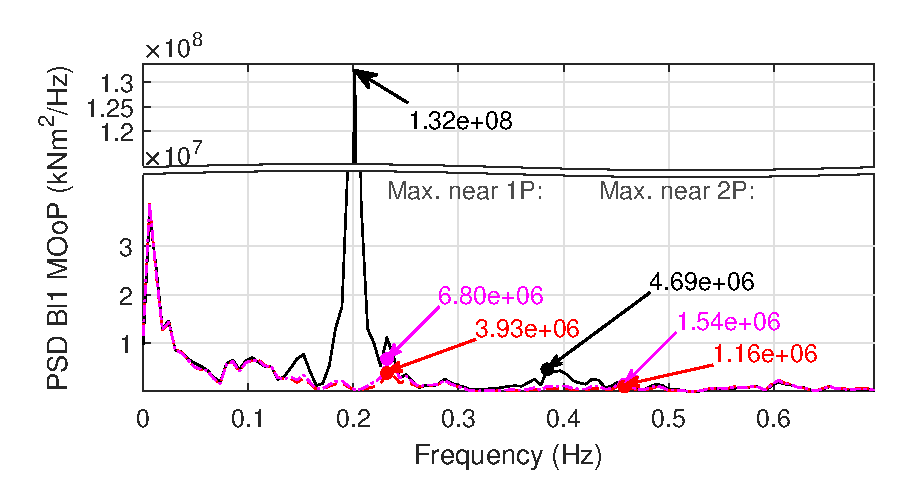
\includegraphics[width=0.65\textwidth]{figures/figIPCThesis/fig02_PSDroot_breaky1c_AALC.eps}}
    \caption[Controller comparison: Power Spectral Density of the blade~1 root out-of-plane moment of baseline PI, IPC, TEFC, AALC, and AALC with optimized parameters.]{Controller comparison: Power Spectral Density of the blade~1 root out-of-plane moment of baseline PI, IPC with $K_{\text{I,IPC}} = 1$, TEFC with $K_{\text{P,TEFC}} = 1$, AALC with $K_{\text{I,IPC}} = 1$ and $K_{\text{P,TEFC}} = 1$, and AALC with optimized parameters \(K_{\text{P,IPC}}\), \(K_{\text{I,IPC}}\), and \(K_{\text{P,TEFC}}\), see Table~\ref{tabone}. Results for turbulent wind (18 m/s mean, turbulence class A, optimization dataset).}
    \label{fig:PSDTEF}
\end{figure}
%
IPC (blue line) and TEFC (green line) reduce the PSD of the 1P and 2P loads, respectively, compared to the baseline (black line): IPC alone reduces the 1P peak by 97.4\%, but increases the 2P peak by 29.8\%, while TEFC alone reduces the 2P peak by 76.8\% and the 1P peak by 38.3\%. These PSDs are obtained with the initially used AALC parameters with the original setting of a purely integral IPC and a purely proportional TEFC feedback, both set to values of one. In a second step, the three parameters \(K_{\text{P,IPC}}\), \(K_{\text{I,IPC}}\), and \(K_{\text{P,TEFC}}\) are optimized at 18\,m/s, subject to the constraint that the tower base DEL does not exceed that of the baseline, resulting in an IPC PI controller with $K_{\text{P,IPC}} = 0.082$ and $K_{\text{I,IPC}} = 0.669$ and a TEFC P controller with $K_{\text{P,TEFC}} = 0.641$. An optimization started from the initial parameters instead of the optimized IPC parameters converges to the same cost.

Figure~\ref{fig:PSDTEF}\,(b) demonstrates that considerable improvement with respect to the baseline controller is possible using the suggested AALC design: The combined IPC-TEFC with the original setting of a purely integral IPC and proportional TEFC feedback reduces the PSD at 1P by 97.0\%, and at 2P by 75.3\%. With the optimized parameters, the reduction with respect to the baseline is 94.9\% at 1P and 67.3\% at 2P, i.e., the residual peaks are larger than with the initial setting. The cost function, the largest of the three blade DELs, is nevertheless decreased from $J = 0.778$ for the initial controller to $J = 0.773$ for the optimized one, as the optimized controller reduces the DELs of the three blades more evenly (by 22.7\% to 23.3\%, compared to 22.2\% to 25.1\% with the initial setting). At the same time, the optimized AALC requires less pitch activity than the optimized IPC without TEF: the standard deviation of the pitch rate is 2.14\textdegree/s compared to 2.98\textdegree/s.
From this study, it seems unlikely that a parameter optimization of the suggested, carefully designed controller can decrease the blade damage equivalent loads considerably further. Further investigations might be made with respect to how much improvement is achievable with a more sophisticated MIMO controller.

%
Table~\ref{tabone} contains six evaluation criteria to quantify the effect of the AALC: blade, tower base, and tower top DEL, mean of generated power $\bar{P}_{g}$, its standard deviation $\delta P$, and actuator power $C_{\text{Act}}$, Equation~\eqref{eq:CAct}, normalized by simulations without AALC for the same wind test cases. These are the criteria provided in Section~\ref{sec:ControllerParameterOptimization}, which are the same objectives shown for IPC without TEFs in Table~\ref{tab:IPC_summary} for wind speed ranges for above rated wind. For that table, the parameters are fixed. Here they vary as follows:
\begin{itemize}
    \item For wind speeds of 10\,m/s and above, the parameters optimized at 18\,m/s ($K_{\text{P,IPC}} = 0.082$, $K_{\text{I,IPC}} = 0.669$, and $K_{\text{P,TEFC}} = 0.641$) are used.
    \item For the datasets with wind speeds of 4\,m/s, 6\,m/s, and 8\,m/s, the AALC parameters are scheduled with the parameters optimized separately. The parameters were set to
    \begin{itemize}
        \item for  4\,m/s to $K_{\text{P,IPC}} = 0.422$,  $K_{\text{I,IPC}} = 0.959$,  $K_{\text{P,TEFC}} =  2.028$,
        \item for  6\,m/s to $K_{\text{P,IPC}} =2.038$,  $K_{\text{I,IPC}} = 1.437$,  $K_{\text{P,TEFC}} = 2.970$, and
        \item for  8\,m/s to $K_{\text{P,IPC}} =-0.043$,  $K_{\text{I,IPC}} = 0.826 $,  $K_{\text{P,TEFC}} = 4.939$.
    \end{itemize}
\end{itemize}
These controllers are applied on FAST and the criteria are calculated from the obtained closed-loop data. Averages over five wind speed ranges are derived: all wind speeds, the wind speeds below and above rated, the wind speeds from 18\,m/s, and the optimization wind speed of 18\,m/s. Unlike in \cite{dittmer2024combined}, where W\"ohler exponents of 8 and 3 were used, the DELs are calculated with the exponents of 10 and 4 used throughout this thesis and evaluated from 60\,s onward, so that the values differ from those published there.
% \caption[Evaluation criteria for IPC: Mean values of the optimization and verification datasets over above rated wind speed ranges]{\label{tab:IPC_summary} Evaluation criteria for IPC: Mean values of the optimization and verification datasets over above rated wind speed ranges, normalized by the baseline PI without IPC; values below 1 indicate a reduction. IPC gains optimized at 18\,m/s with the pitch rate limit 8\textdegree/s for all wind speeds: $K_{\text{P,IPC}} = 1.222$ and $K_{\text{I,IPC}} = 0.370$. Criteria are blade, tower base and tower top DELs, power mean and standard deviation, and pitch actuator power. The first verification set has no wind field for 13\,m/s.}

% Created by makeAALC_SummaryTable on 2026-10-26
\begin{table}[h]
    \centering
    
    \caption[Evaluation criteria for AALC: Mean values of the optimization and verification datasets over different wind speed ranges.]{Evaluation criteria for AALC: Mean values of the optimization and verification datasets over different wind speed ranges, normalized by the baseline PI; values below 1 indicate a reduction. From 10\,m/s on, the AALC gains optimized at 18\,m/s are used: $K_{\text{P,IPC}} = 0.082$, $K_{\text{I,IPC}} = 0.669$ and $K_{\text{P,TEFC}} = 0.641$; below, the gains are scheduled with the gains optimized at 4, 6 and 8\,m/s. Criteria are blade, tower base and tower top DELs, power mean and standard deviation, and pitch actuator power (not given below rated, where the baseline actuator power is close to zero). The first verification set has no wind fields for 11 and 13\,m/s.}
    \begin{tabular}{@{}l*{8}{c}@{}}
        \toprule
        Wind speeds & Dataset & Turb. class & $C_{\text{DEL},b}$ & $C_{\text{DEL},t,\text{Base}}$ & $C_{\text{DEL},t,\text{Top}}$ & $C_{\bar{P}}$ & $C_{\delta P}$ & $C_{\text{Act}}$ \\
        \midrule
        \multirow{3}{*}{All (4--25\,m/s)} & Optim. & A & 0.77 & 0.98 & 0.89 & 0.99 & 1.02 & 4.54 \\
        & Verif. 1 & A & 0.84 & 0.98 & 0.91 & 0.99 & 1.00 & 4.60 \\
        & Verif. 2 & B & 0.80 & 0.99 & 0.89 & 0.99 & 1.00 & 4.73 \\
        \midrule
        \multirow{3}{*}{\begin{tabular}[c]{@{}l@{}}Below rated\\(4--11\,m/s)\end{tabular}}& Optim. & A & 0.80 & 0.94 & 0.89 & 0.98 & 1.00 & -- \\
        & Verif. 1 & A & 0.98 & 0.93 & 0.93 & 0.97 & 0.98 & -- \\
        & Verif. 2 & B & 0.84 & 0.96 & 0.89 & 0.98 & 0.98 & -- \\
        \midrule
        \multirow{3}{*}{\begin{tabular}[c]{@{}l@{}}Above rated\\(12--25\,m/s)\end{tabular}} & Optim. & A & 0.76 & 1.00 & 0.89 & 1.00 & 1.02 & 3.86 \\
        & Verif. 1 & A & 0.77 & 1.00 & 0.90 & 1.00 & 1.01 & 3.85 \\
        & Verif. 2 & B & 0.78 & 1.01 & 0.89 & 1.00 & 1.02 & 4.02 \\
        \midrule
        \multirow{3}{*}{18--25\,m/s} & Optim. & A & 0.74 & 1.00 & 0.90 & 1.00 & 1.00 & 3.99 \\
        & Verif. 1 & A & 0.74 & 1.00 & 0.92 & 1.00 & 1.00 & 3.89 \\
        & Verif. 2 & B & 0.73 & 1.02 & 0.91 & 1.00 & 1.00 & 4.19 \\
        \midrule
        \multirow{3}{*}{18\,m/s} & Optim. & A & 0.79 & 1.00 & 0.86 & 1.00 & 0.99 & 3.64 \\
        & Verif. 1 & A & 0.79 & 1.00 & 0.90 & 1.00 & 1.00 & 3.49 \\
        & Verif. 2 & B & 0.78 & 1.06 & 0.87 & 1.00 & 1.00 & 3.77 \\
        \bottomrule
    \end{tabular}
    \label{tabone}
\end{table}

While load reduction is also achievable below rated wind speed, Table~\ref{tabone} shows that the control parameters that worked well on the optimization set reduced the loads on the first verification set only marginally: the blade DEL is reduced by 20\% for the optimization set and by 16\% for the second verification set, but only by 2\% for the first verification set, i.e., the parameters optimized below rated do not carry over reliably to other wind fields. As the baseline pitch angle is almost constant for below rated wind speeds, the baseline actuator power is close to zero and no meaningful ratio is obtained for the actuator criterion. Nevertheless, some improvements can be seen: the tower base DEL is reduced by 4\% to 7\% and the tower top DEL by 7\% to 11\%. For all datasets, a decrease in power is observed: the mean power is decreased by 2\% to 3\%, as the flap and pitch deflections reduce the aerodynamic efficiency, see Figure~\ref{fig:OLval}. This makes the application of TEFs during periods with below rated wind speeds economically non-viable. No further investigation of finding suitable controller parameters for this range is hence conducted.

The following analysis focuses on the above rated wind speed ranges. The reduction values achieved with IPC without TEFs from Table~\ref{tab:IPC_summary} are also provided here for direct comparison. The blade root out-of-plane moments, quantified with the criterion $C_{\text{DEL},b}$, the sum of the blade DELs, decrease as follows:
\begin{itemize}
    \item For the mean value of all above rated wind speeds, compared to the baseline PI, the blade DEL criterion $C_{\text{DEL},b}$ decreases by 22\% (on the second verification set) to 24\% (on the optimization set). The corresponding reductions achieved by IPC are 21\% to 23\%. 
    \item If only wind speeds from 18\,m/s on are considered, the loads are decreased by 26\% (on the two sets with turbulence class A) to 27\% (on the set with turbulence class~B), with the corresponding reduction range for IPC being 24\% to 25\%.
    \item Finally, if only the runs with a wind speed of 18~m/s are considered, which includes the optimization set that was used to derive the controller parameters, the reduction amounts to 21\% to 22\%, with the largest reduction again observed for the second verification set of turbulence class~B. 
\end{itemize} 
Including all wind speeds, the blade DEL is reduced by 16\% to 23\%. The parameters optimized at a single wind speed carry over to the whole of Region~III and to both verification sets, so that no gain scheduling is required above rated. Compared to the load reduction achieved with IPC, a small further improvement of up to 2 percentage points is observed for the objective $C_{\text{DEL},b}$.
%
Regarding the tower DELs, quantified with the objectives $C_{\text{DEL},t,\text{Base}}$ and $C_{\text{DEL},t,\text{Top}}$, the following influence of the AALC is observed:
\begin{itemize}
    \item The tower base DEL is not changed considerably above rated, with criteria between 1.00 and 1.01; the largest increase of a single wind speed is 6\% at 18\,m/s for turbulence class~B. Above rated and at 18\,m/s, the IPC values in Table~\ref{tab:IPC_summary} happen to be identical to the AALC ones in Table~\ref{tabone} for this objective.
    \item The tower top DEL, in contrast, is reduced by 10\% to 11\% on average above rated, 8\% to 10\% for the wind speed range above 18\,m/s, and by 10\% to 14\% at 18\,m/s. This is noticeably more than by the IPC alone, where the corresponding numbers are 7\% above rated, 5\% to 7\% and 8\% to 10\%. 
\end{itemize}
%
The evaluation of the power criteria confirms that the AALC leads only to negligible changes in both power mean and variance above rated. The additional movement of the blade demanded by the IPC component of the AALC is the only criterion leading to an unavoidable increase, similar to the IPC scheme discussed in the previous sections. However, the objective $C_{\text{Act}}$ is another criterion where AALC outperforms IPC: 
\begin{itemize}
    \item Above rated, the actuator power is increased by a factor of 3.9 to 4.0, and from 18\,m/s on by a factor of 3.9 to 4.2. The corresponding values for IPC are 5.4 to 5.7, and 5.8 to 6.0.
    \item If only the simulations at a wind speed of 18\,m/s are considered, these values are lower as the additional actuator demand increases with higher wind speeds: They are 3.5 to 3.8 for AALC and 5.0 for IPC.
\end{itemize}
In summary, when considering above-rated wind speeds, AALC outperforms IPC: it provides an additional reduction in blade DELs of up to 2 percentage points and in tower top DELs of up to 4 percentage points, and it decreases the actuator criterion $C_{\text{Act}}$ by about 30\%. To assess the overall performance of AALC and IPC with regard to the qLMPC CPC scheme, the following section presents a comparison of all three investigated algorithms on load reduction and power standard deviation at different pitch rate limits.


%The resulting closed loop simulation results are referred to in this chapter as qLMPC (Mdl2), qLMPC (FAST) and qLMPC smooth (FAST). All of them were tested with three different pitch rate limits,  4\textdegree/s, 8\textdegree/s, and 13\textdegree/s.
%\item 

\section{Comparison of Wind Turbine Control Designs}
\label{subsec:ComparisonWindTurbineControlDesigns}

Three different control approaches were discussed in this chapter: In Section~\ref{sec:quasiLPVMPCDesign} a qLMPC algorithm was presented and applied to a qLPV model without any model mismatch as well as to FAST. Tested on the qLPV model, it resulted in considerable reduction of the standard deviation of the tower fore-aft acceleration, rotor speed and power. It was shown that there is a trade-off between these objectives and pitch actuation by testing the qLMPC with three different pitch rate limits, but that the qLMPC outperformed the baseline PI at all three rate limits. However, when tested on FAST, the original design performed considerably worse regarding rotor speed and power. Some of the performance improvement could be recovered by adapting and enhancing the MPC. 

Section~\ref{section:Individal Pitch PI Control} presented the optimization of an IPC PI controller that was run in addition to the baseline PI controller. Its performance was also tested with the three pitch rate limits. In Section~\ref{sec:CombinedIPC-TrailingEdgeFlapControl} the addition of TEFs was shown. Optimization of a proportional gain for these additional control surfaces was discussed and the resulting AALC was shown to slightly outperform the IPC with regard to DEL reduction and considerably with regard to actuator activity. The decision was made to only tune the AALC scheme for the standard pitch rate of 8\textdegree/s, which is widely used in the literature, as the IPC exceeds this rate limit only rarely.

This section presents the combination of the qLMPC designs from Section~\ref{sec:quasiLPVMPCDesign} with the IPC implementation from Section~\ref{section:Individal Pitch PI Control} as another approach to alleviate the blade loads as well as reduce power standard deviation at an acceptable increase in actuator activity.
%\end{itemize}
The results achieved with the qLMPC can be summarized as follows. In a first simulative analysis, the qLMPC was evaluated on the simplified qLPV turbine model that is also
used as its prediction model, for turbulent wind with a mean of 18\,m/s. Without any model
mismatch, this qLMPC (Mdl2) data showed large improvements over the PI baseline across all evaluated pitch rate limits.
As presented in Table~\ref{tab:stddev_unified}, 
\begin{list}
    {-}{\setlength{\topsep}{5pt}\setlength{\partopsep}{5pt}\setlength{\itemsep}{0pt}\setlength{\parsep}{0pt}}
    \item the standard deviation of the tower fore-aft acceleration was reduced
    by factors of 2.58, 3.82, and 4.14 for the pitch rate limits of 4\textdegree/s, 8\textdegree/s, and
    13\textdegree/s, respectively.
    %\item  This corresponds  corresponding to reductions of 61\%, 74\%, and 76\% relative to the PI baseline at 8\textdegree/s). 
    \item Similarly, the power error standard deviation dropped dramatically
    by factors of 6.42, 10.29, and 11.35 (reductions between 84\% and 91\%), 
    \item and the rotor speed
    standard deviation showed matching improvements with reductions up to a factor of 11.40 at the
    13\textdegree/s rate limit. 
\end{list}
These improvements did not hold up when the controller was applied to the FAST model of the NREL 5MW
turbine. The original qLMPC design increased the power tracking error instead of reducing it, mainly due to the single-point hub height wind speed used for scheduling, while the FAST rotor averages the fluctuations of a full wind field, and additionally due to the modes of FAST, which are not contained in the prediction model.
%
The improvements were partly recovered with several modifications, namely rotor speed tracking, a prediction model extended by the tower fore-aft and blade flap dynamics, a controller sample time of 0.04\,s, scheduling with the rotor-effective wind speed, notch filters in the measured speeds at the 3P frequency and the drivetrain mode, as well as, for the smooth design, a controller sample time of 0.12\,s and a ramped pitch reference.
%
The smooth design, enhanced with these extensions, reduces the power variance on FAST again. However, the increase in tower
loads was only partially reduced, and the tower DELs remained higher than those obtained with the baseline PI controller. Note that on the simplified model implemented in Simulink, the
rotor-effective wind filters shown in Table~\ref{tab:stddev_unified} have a similar effect: they
remove a large part of the wind excitation. With this, the pitch activity was reduced below that of the baseline PI, but there was a decrease in improvement of the
qLMPC regarding tower acceleration and power standard deviation reduction. 
%
Therefore, the notch filter and smooth designs are combined with the IPC of Section~\ref{section:Individal Pitch PI Control}, with the gains scaled as described in Section~\ref{sec:qLMPCFAST}. Figure~\ref{fig:CtrlCmpFASTIPC} and Table~\ref{tab:CtrlComparisonFASTNTM18B_PI_flapNotch_flapNotchIPC} show the effect of the IPC on the qLMPC notch filter and smooth designs in the time domain. The turbulent wind field of Section~\ref{quasiLPVMPCResults} and a pitch rate limit of 13\textdegree/s are used. Note that the bar and Pareto plots below are based on the second verification set and a pitch rate limit of 8\textdegree/s.
The following can be observed from Figure~\ref{fig:CtrlCmpFASTIPC} where the baseline PI is depicted as a blue line, the qLMPC design as an orange line, and the combination of qLMPC and IPC as a yellow line. Table~\ref{tab:CtrlComparisonFASTNTM18B_PI_flapNotch_flapNotchIPC} summarizes the findings from the comparison of the five controller setups:
\begin{itemize}
    \item All four qLMPC algorithms show a considerable decrease in the standard deviation of rotor speed and power tracking error: Compared to the baseline PI, the standard deviations of the rotor speed and of the power tracking error are reduced by factors of 3.8 and 3.3 without IPC and of 3.7 and 3.3 with IPC. For the smooth design, the factors are 2.1 and 2.0 without and 2.2 and 2.0 with IPC. Regarding these criteria, adding the IPC has little influence on the already good improvement.
    \item  The tower acceleration and the tower base DEL increase slightly further by 4\%: without IPC, they are increased by 35\% and 27\%, with IPC by 40\% and 31\%. For the smooth design, the increases are smaller, 16\% and 12\% without and 20\% and 15\% with IPC.
    \item  However, the qLMPC-IPC, like the PI IPC, reduces the standard deviation of the blade root out-of-plane moment by 23\% and the blade DEL by 18\%, i.e.\ to 14\% below that of the baseline PI controller. For the smooth design, the reductions are 23\% and 19\%, i.e.\ to 19\% below the baseline. 
    \item The trade-off is that adding the IPC increases the blade 1 pitch rate by 15\%, to 6.2 times that of the baseline PI (5.4 without IPC). For the smooth design, the pitch rate is considerably lower, 2.3 times that of the baseline without and 3.9 times with IPC.  
\end{itemize}
Both combined qLMPC-IPC designs are thus able to reduce the power standard deviation and the blade DEL. The latter was not achieved with the qLMPC with collective pitch control. However, these improvements come at the price of a further, albeit small, increase in tower DEL and a considerable increase in pitch rate, both of which are smaller for the smooth design.
%
\begin{figure} [htbp]
    \subfloat[Notch filter design]{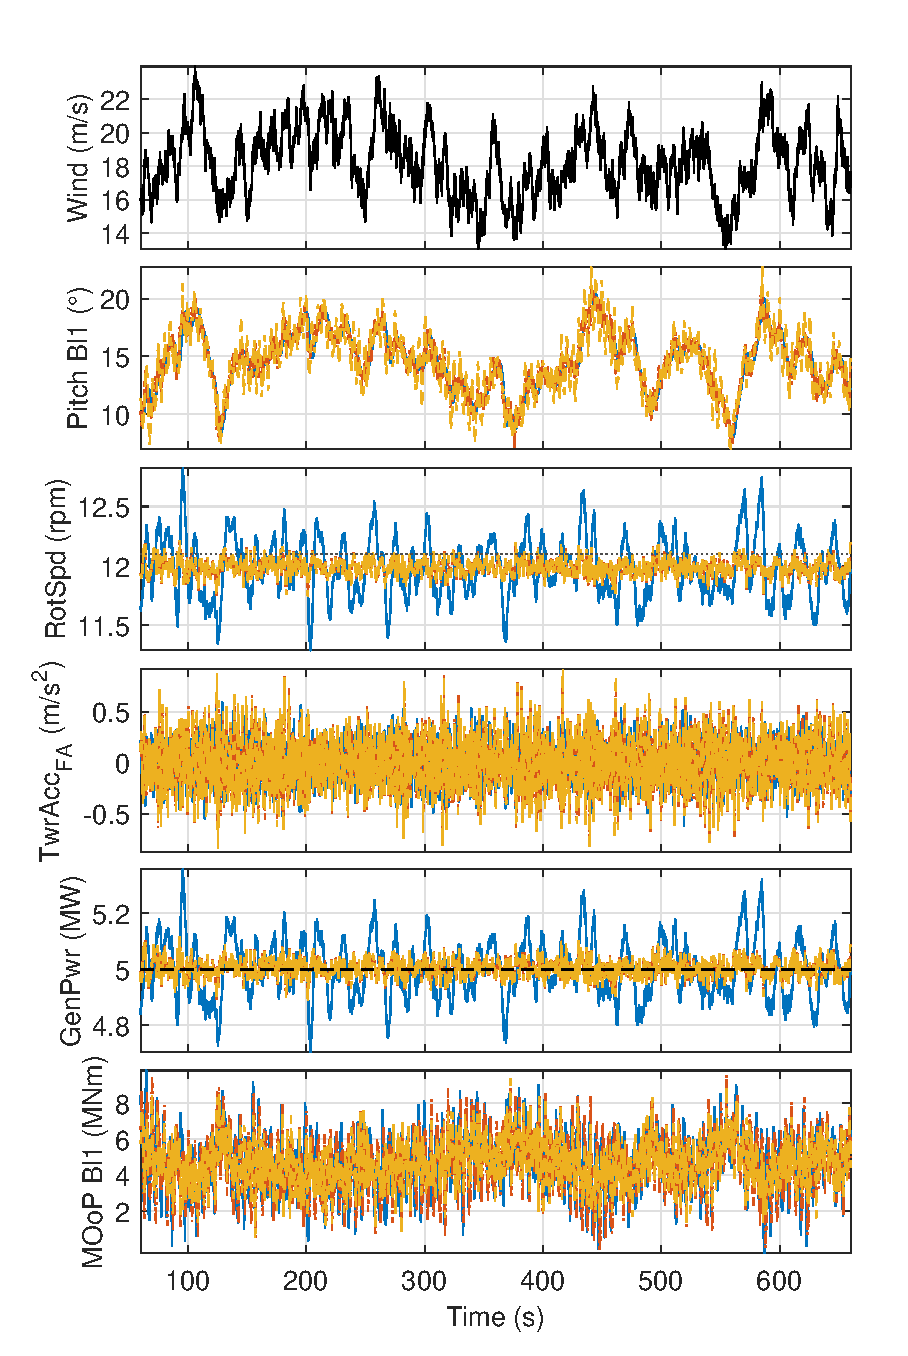
\includegraphics[width=0.495\textwidth,trim={0.cm 0cm 0cm 0.5cm}, clip]{figures/figDirFASTthesis/cmpCtrlFASTthesis_NTM18B_PI_flapNotch_flapNotchIPC.eps}}\hfill
    \subfloat[Smooth design]{\includegraphics[width=0.495\textwidth,,trim={0.cm 0cm 0cm 0.5cm}, clip]{figures/figDirFASTthesis/cmpCtrlFASTthesis_NTM18B_PI_flapNotchSmooth12_flapNotchSmooth12IPC.eps}}\hfill
    \caption[Controller comparison on FAST: baseline PI vs. qLMPC designs without and with IPC for turbulent wind (18\,m/s mean, turbulence class B).]
    {Controller comparison on FAST: baseline PI (\mlBlue) vs. qLMPC designs without (\mlOrange) and with IPC (\mlYellow) for turbulent wind (18\,m/s mean, turbulence class B), pitch rate limit 13\textdegree/s. Displayed signals: freestream wind speed, generator torque, blade 1 pitch angle, rotor speed, tower fore-aft acceleration, generator power with its reference (\mlBlackDashed), and blade 1 root out-of-plane moment.}
    \label{fig:CtrlCmpFASTIPC}
\end{figure}
%
\begin{table}[htbp]
    \centering
    \small
    \setlength{\tabcolsep}{4pt}
    \caption[Controller comparison on FAST, 18\,m/s turbulent (class B): notch filter design and smooth design, each without and with IPC.]{Controller comparison on FAST v8.16, 18\,m/s turbulent (class B), pitch rate limit 13\textdegree/s, notch filter design and smooth design, each without and with IPC. Top: standard deviations of the tower fore-aft acceleration, the power tracking error, the rotor speed, the blade 1 pitch rate (differenced over 0.04\,s), and the blade root out-of-plane (OoP) moment (mean of the blades). Bottom: damage equivalent loads of the tower base (W\"ohler exponent 4) and the blade root (exponent 10, maximum of the blades). Values in parentheses: ratio of the baseline PI value to the controller value; values above 1 indicate an improvement. Best values are marked in bold.}
    \label{tab:CtrlComparisonFASTNTM18B_PI_flapNotch_flapNotchIPC}
    \begin{tabular}{l rrrrr}
        \toprule
        &  & \multicolumn{2}{c}{Notch filter design} & \multicolumn{2}{c}{Smooth design} \\
        \cmidrule(lr){3-4} \cmidrule(lr){5-6}
        Signal & Baseline PI & w/o IPC & w/ IPC & w/o IPC & w/ IPC \\
        \midrule
        Tower acc.\ (m/s$^2$) & \textbf{0.1712} & 0.2310 (0.74) & 0.2393 (0.72) & 0.1990 (0.86) & 0.2046 (0.84) \\
        Power error (kW) & 59.60 & \textbf{17.90 (3.33)} & 18.08 (3.30) & 29.18 (2.04) & 29.08 (2.05) \\
        Rotor speed (rpm) & 0.2460 & \textbf{0.0653 (3.77)} & 0.0660 (3.73) & 0.1145 (2.15) & 0.1141 (2.16) \\
        Blade 1 pitch rate (\textdegree/s) & \textbf{0.50} & 2.71 (0.18) & 3.11 (0.16) & 1.16 (0.43) & 1.93 (0.26) \\
        Blade root OoP moment (kNm) & 1574 & 1559 (1.01) & 1207 (1.30) & 1548 (1.02) & \textbf{1188 (1.32)} \\
        \midrule
        Tower base DEL (kNm) & \textbf{15394} & 19493 (0.79) & 20232 (0.76) & 17172 (0.90) & 17728 (0.87) \\
        Blade root DEL (kNm) & 6002 & 6249 (0.96) & 5145 (1.17) & 6019 (1.00) & \textbf{4871 (1.23)} \\
        \bottomrule
    \end{tabular}
\end{table}
%
All seven designs are compared for the same wind, the turbulent 18\,m/s wind of the
second verification set (IEC turbulence class~B), with the pitch rate limits 4\textdegree/s,
8\textdegree/s, and 13\textdegree/s. The qLMPC is evaluated on the simplified model Mdl2 as the
ideal case without model mismatch, and on FAST with the filter designs, both on their own
and combined with the individual pitch controller of Section~\ref{section:Individal Pitch PI Control}.
IPC and AALC are evaluated on OpenFAST with the optimized gains for each rate limit and the
AALC gains of Section~\ref{subsec:ResultsTEF} at 8\textdegree/s. All criteria are normalized by the
PI baseline on the same plant and with the same pitch rate limit, so values below unity
indicate an improvement. The blade DEL and the DELs of the tower base and the tower top fore-aft moments are computed by
rainflow counting with W\"ohler exponents of 10 for the blades, summed over the three blades, and
4 for the steel tower; all criteria are evaluated from 60\,s onwards to exclude the start-up. Mdl2 contains neither blade loads nor a pitch moment.


For the qLMPC on Mdl2, the standard deviation of the
tower top fore-aft acceleration replaces the tower base DEL, no blade and tower top DELs are given, and $C_\text{Act}$ is calculated with a pitch moment estimated from the pitch angle, its derivatives, and the wind speed, fitted by least squares to the pitch moment of blade~1 in the FAST runs of the PI and the notch filter design at 8\textdegree/s. The fit explains only a quarter of the variance of the pitch moment ($R^2 = 0.25$); most of the remaining variance lies around the rotational frequency 1P, which depends on the blade azimuth and cannot be represented by the collective signals of Mdl2. The actuator power is nevertheless reproduced within 0.3\% for the qLMPC designs on FAST, as the pitch moment is dominated by its nearly constant mean value of about $-86$\,kNm, which is the same for all controllers. $C_\text{Act}$ is therefore essentially the ratio of the mean absolute pitch rates: on FAST, the two differ by less than 2\%, and for the qLMPC on Mdl2 by less than 0.5\%.

Figure~\ref{fig:CtrlCompBarPareto}(a) shows the evaluation criteria of all controllers at the standard
pitch rate limit of 8\textdegree/s, grouped by controller. It is important to note that no controller changes the mean power
$C_{\bar{P}}$ depicted in gray as the fourth bar; all values are within 0.5\% of the baseline and hence, with only the first two digits displayed, the bar appears to be exactly at the value of one for all seven algorithms. Figure~\ref{fig:CtrlCompBarPareto}(b) disregards the mean power criterion and visualizes the three DEL criteria and the power standard deviation as functions of the actuator power for all three pitch rate limits. Each line connects the
results of one controller for the rate limits of 4\textdegree/s, 8\textdegree/s, and 13\textdegree/s,
indicated by white, gray, and black marker fill. The AALC was optimized for 8\textdegree/s only and
is therefore represented by a single point per criterion. Results closer to the lower left corner
are better, as they combine lower loads or power variance with less actuator activity. Each panel
highlights one group of controllers and shows the others pale for reference.

\begin{figure}[htbp]
    \centering
    \subfloat[Bar plot at a pitch rate limit 8\textdegree/s\label{fig:EvalCrit1}]{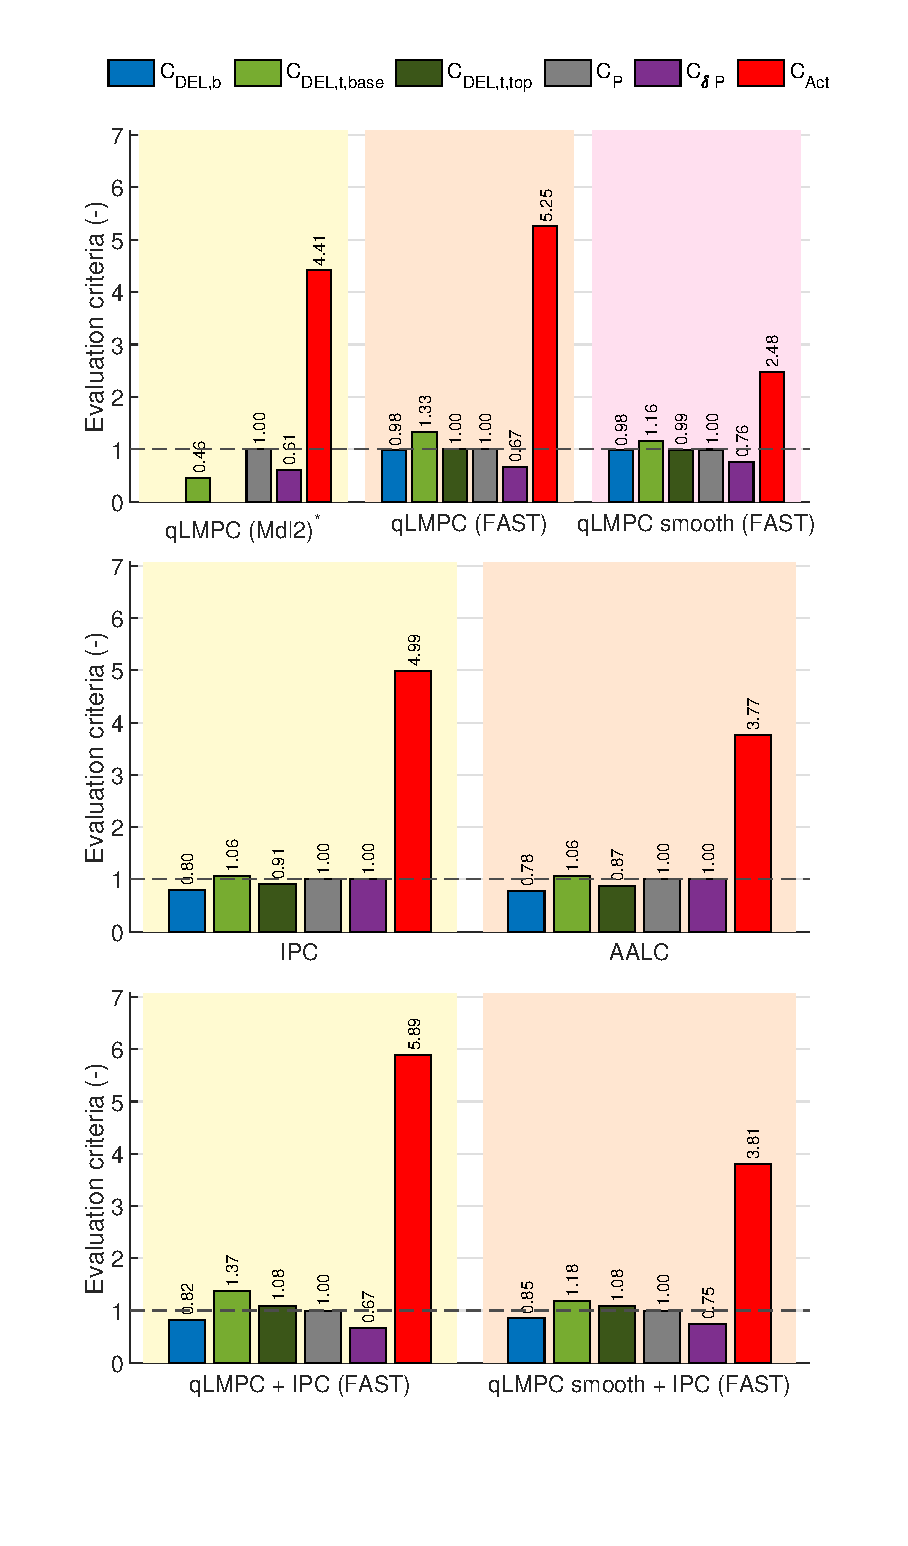
\includegraphics[width=0.499\textwidth]{figures/figures_WESC25/afig01_IPCMPCbar.eps}}\hfill
    \subfloat[Pareto plot\label{fig:CtrlCompAll}]{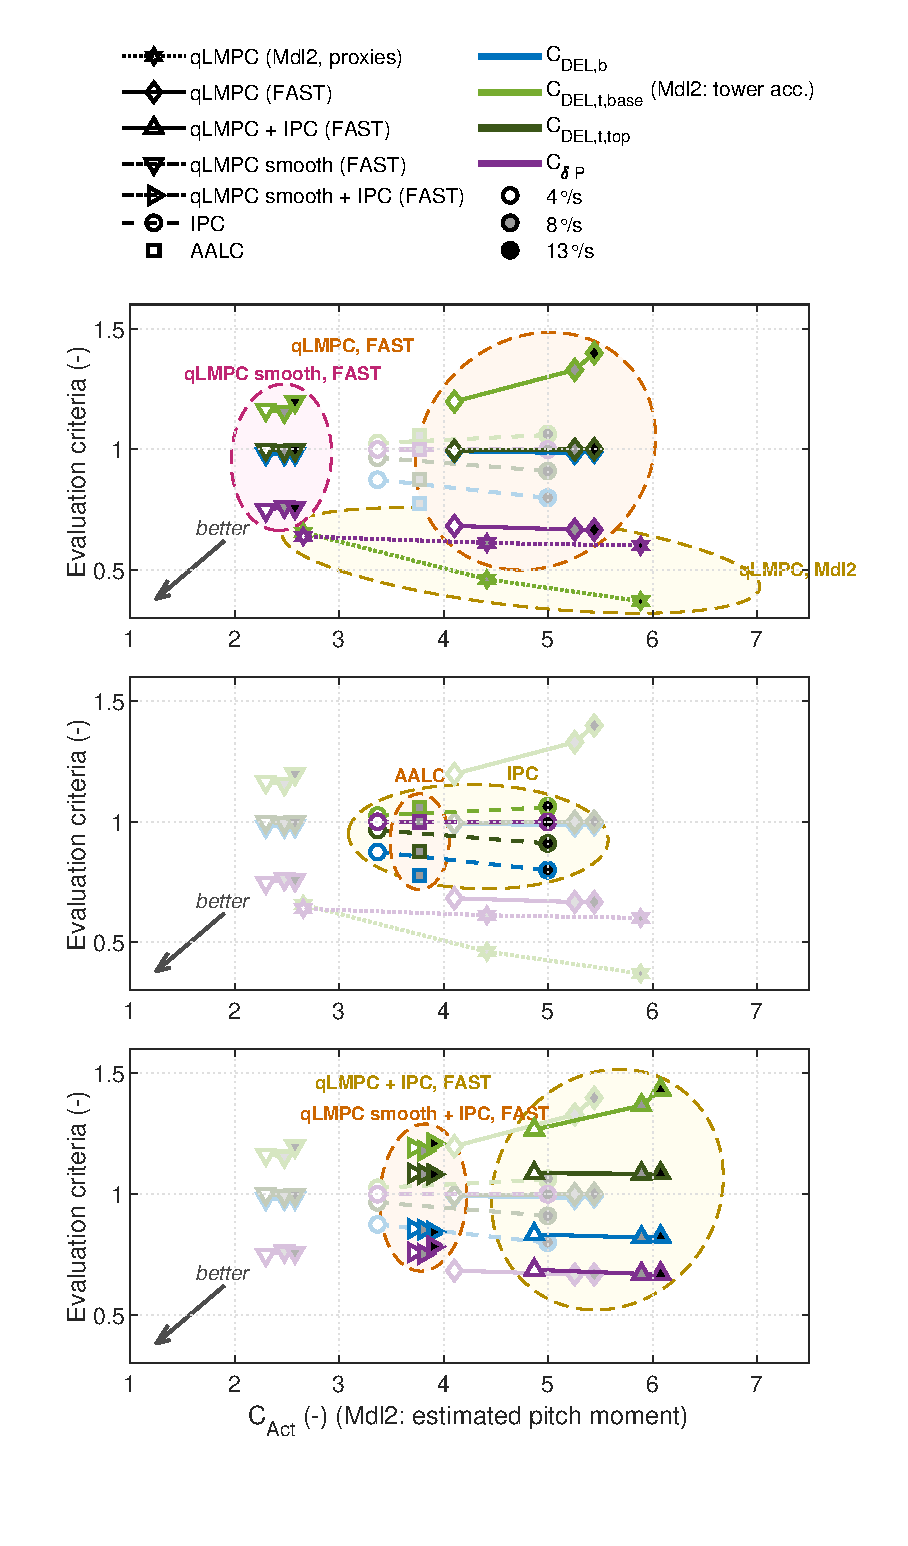
\includegraphics[width=0.499\textwidth]{figures/figures_WESC25/afig01_IPCMPCpareto.eps}}
    \caption[Evaluation criteria of qLMPC, IPC, and AALC for turbulent wind]{Evaluation criteria of the controllers for turbulent wind (18\,m/s mean, IEC turbulence class~B, second verification set), normalized by the PI baseline with the same pitch rate limit. Panels: qLMPC (top), IPC and AALC (middle), qLMPC combined with IPC (bottom). (a)~Bar plots: blade DEL $C_{\mathrm{DEL},b}$, tower base and top DELs $C_{\mathrm{DEL},t,\mathrm{Base}}$ and $C_{\mathrm{DEL},t,\mathrm{Top}}$, mean power $C_{\bar{P}}$, power standard deviation $C_{\delta P}$, and actuator power $C_\text{Act}$. (b)~Pareto plot: $C_{\mathrm{DEL},b}$ (blue), $C_{\mathrm{DEL},t,\mathrm{Base}}$ (green), $C_{\mathrm{DEL},t,\mathrm{Top}}$ (dark green), and $C_{\delta P}$ (purple) over $C_\text{Act}$ for the pitch rate limits 4\textdegree/s (white markers), 8\textdegree/s (gray), and 13\textdegree/s (black); the controllers of the other panels are shown pale. The dashed ovals enclose all points of one controller; their color matches the background of the same controller in the same panel of the bar plot. The qLMPC on Mdl2 (no model mismatch): tower top fore-aft acceleration instead of the tower base DEL, no blade and tower top DELs, $C_\text{Act}$ with the pitch moment estimated from a model fitted to FAST. The arrow points towards better results.}
    \label{fig:CtrlCompBarPareto}
\end{figure}
The two top panels show the qLMPC schemes. On Mdl2, i.e.\ without model mismatch (yellow background), the power standard deviation is reduced by 39\% and the standard deviation of the tower fore-aft acceleration by 54\%. This is the setup used in \cite{dittmer2021velocity} to investigate the potential of the velocity-based qLMPC. The Verif.~2 wind field differs from the test case of Section~\ref{quasiLPVMPCResults} and falls below rated wind speed several times, so the improvements are smaller than the 74\% and 90\% reported there at 8\textdegree/s. The actuator power increases by a factor of 4.4, as the qLMPC compensates the wind fluctuations with fast pitch action, which might well be worth the additional actuator usage. These improvements, however, could not be replicated on FAST (orange background): the qLMPC with notch filters still reduces the power standard deviation by 33\%, but increases the tower DEL by 33\% and requires the highest actuator power of all controllers without IPC, 5.3 times that of the PI baseline. The smooth design (pink), which uses a longer controller sample time and a ramped pitch reference to make the qLMPC less aggressive, trades part of the power smoothing, a reduction by 24\%, for considerably less pitch activity: its actuator power of 2.5 is the lowest of all controllers, and the tower DEL increase is halved to 16\%.

The middle panels visualize the IPC and the AALC, which act on the blade loads. The IPC, highlighted with a wider, yellowish oval as it was optimized for each rate limit, reduces the blade DEL from 0.87 at 4\textdegree/s to 0.80 at 8\textdegree/s; 13\textdegree/s brings no further benefit, as the gains optimized for 13\textdegree/s and 8\textdegree/s are almost identical. The tower DEL increases slightly with the rate limit, from 1.03 to 1.06, and the power standard deviation remains at unity. The AALC lies below the IPC curve, i.e., it achieves the larger blade load reduction at a lower pitch actuator power, 3.8 compared with 5.0, as the trailing edge flaps take over part of the load reduction. This is its main advantage, as the further reduction is only 2\% for the blade DEL and 4\% for the tower top DEL.

The bottom panels depict the combination of qLMPC and IPC. Compared with the pale qLMPC curves, adding IPC mainly shifts the blade DEL downwards and the actuator power to the right, while the tower base DEL and the power standard deviation hardly change and the tower top DEL increases by about 8\%. The smooth design combined with IPC lies at about the actuator power of the AALC, 3.8, and below that of the IPC, 5.0. Its blade DEL of 0.85 comes close to the 0.80 of the IPC alone, and it additionally reduces the power standard deviation by about 25\%, which neither IPC nor AALC achieve. As the IPC gains were only scaled by hand on the notch filter design and not retuned for the smooth design (Section~\ref{sec:qLMPCFAST}), part of the remaining blade DEL difference may be due to the tuning. Its tower DEL, however, is about 11\% higher than with IPC.

These summary plots show that IPC and AALC are the two investigated approaches suitable for blade load reduction, with AALC achieving the best blade DEL at a moderate actuator power by offloading part of the pitch action onto the trailing edge flaps. The qLMPC is the only approach that reduces the power variance, and it keeps this property in the presence of model mismatch, with a reduction of about a third on FAST compared with about 40\% on Mdl2. Its tower load reduction without model mismatch, however, is lost on FAST, where all qLMPC designs increase the tower DEL. The smooth qLMPC combined with IPC is the most balanced qLMPC variant, reducing both the blade DEL and the power standard deviation at an actuator power comparable to IPC and AALC.
%
These results show that the qLMPC depends on an accurate representation of the wind acting on the rotor and of the turbine dynamics: despite careful tuning and additional filters, the tower DEL reduction could not be transferred to FAST. A relatively low-hanging fruit would be to stitch a qLPV model from linearized FAST models to investigate whether the additional modes reduce the model mismatch and at least partly recover the tower DEL reduction. Furthermore, all qLMPC designs use the hub height wind speed of the wind field, filtered on FAST, i.e., the wind is assumed to be known exactly. Replacing it with an estimate is a necessary next step, while a wind preview, e.g., from a lidar, combined with a better fitting model might further reduce the loads.
%
IPC, in contrast, reduces the loads without wind measurements or additional actuation hardware. The IPC and AALC controllers were tuned to reduce the blade loads and achieved considerable reductions for both the optimization and the verification datasets. The tower DEL, so far only a constraint and evaluation criterion, could additionally be included as an optimization objective. As the AALC reduces the blade DEL only 2\% more than IPC alone, its main benefit is the lower pitch actuator power, although the power of the flap actuators is not included in this comparison, and it is questionable whether the additional TEF hardware is justified for current turbine sizes. With increasing turbine size, however, reducing the loads without further increasing the actuator power might become more attractive.

The presented qLMPC exploits that individual wind turbine dynamics are well understood and can be described in closed form as low-dimensional nonlinear ODEs. The following chapter discusses data-driven MPC for wind farms, where wake dynamics are time- and location-dependent and cannot be described by closed-form ODEs, yet must be accounted for in any MPC formulation.
    \chapter{Wind Farm Control} \label{sec:ApplicationtoWindFarmControl}

Wind turbines are grouped into farms to efficiently use locations suitable for wind energy harvesting. Within a wind farm, as many turbines as economically viable are installed, with their number limited by wake interactions. A higher turbine density per area reduces the cost of grid connection per turbine and lowers operation and maintenance costs. However, closely spaced turbines experience wake interactions, causing power losses due to reduced energy availability and increased mechanical loads on downstream turbines.
In \cite{houck2022review} wind farm control methods are surveyed, including Axial Induction Control (AIC), Wake Redirection Control (WRC), their combination, and active wake control. These methods have shown advantages in simulations of varying fidelity, and WRC has also demonstrated benefits in field tests. MPC schemes have been proposed in various studies, such as \cite{spudic2014distMPC_https://doi.org/10.1002/oca.2136, zhao2016coordinated, bay2018active, vali2019adjoint}. Unlike individual turbine dynamics, wake interactions in a wind farm cannot be accurately captured by low-order ODEs. Therefore, the approach applied to wind turbine control in Chapter~\ref{sec:Application to Wind Turbine Control4}, i.e., deriving nonlinear differential equations, creating a qLPV model, and using it for qLMPC control, is not applicable to wind farms. But MPC can be utilized by leveraging data-driven models. Recently, Koopman operator-based methods have proven successful \cite{castillo2020wind, cassamo2021model}. By applying Koopman lifting functions to open-loop simulation data and performing Dynamic Mode Decomposition (DMD), state-space models suitable for MPC algorithms can be obtained. AIC strategies have been developed to handle stationary \cite{sharan2022Koopman} and non-stationary inflow conditions \cite{dittmer2022data}, and a combined WRC-AIC scheme has shown potential for tracking high power demands \cite{dittmer2023koopman}.
%
Section~\ref{sec:WindFarmSimulationWFSim} revisits the design of WFSim, the wind farm simulation tool used in this thesis, describing the modifications and enhancements necessary to model wind speed variations and to represent thrust and power output for turbines with intentional yaw misalignment. Section~\ref{sec:AdaptiveWindFarmqLMPCforAIC} presents an adaptive AIC algorithm capable of handling changes in freestream wind speed. Section \ref{sec:WindFarmLinearMPCforWRC-AIC} first demonstrates wind farm power increases achieved with WRC, followed by a combined WRC-AIC algorithm for grid reference tracking under high power demands. The adaptive AIC scheme, originally published in \cite{dittmer2022data}, and the combined WRC-AIC algorithm, presented in \cite{dittmer2023koopman}, have both been modified to employ predictive models based on control inputs and current power measurements. These modifications eliminate the need for wind measurements for the Koopman MPC during closed-loop simulations of wind farm operation. Furthermore, the lifting functions of the WRC-AIC have been extended to account for the nonlinear influence of the thrust and yaw inputs.

\section{Wind Farm Simulation with WFSim} \label{sec:WindFarmSimulationWFSim}
The wind farm simulation environment WFSim \cite{boersma2017tutorial} is employed both for generating open-loop data and for closed-loop controller testing. A short introduction to WFSim is provided in Section~\ref{sec:WakeModels}, which outlines the background on wind farm models and control. The 2D Navier–Stokes equations (NSE) are described in Section~\ref{Subsection:WindFarmSimulationModels}, and the actuator-disk turbine model is introduced in Section~\ref{Subsection:Windfarmcontrol}. WFSim allows the user to either choose from pre-existing layout definitions and sets of control signals, which may be used in open loop, or introduce new sets. A pre-existing layout of a two-turbine farm was selected, but several excitation signal sets were specifically designed for the studies on which this thesis is based as foundations for Koopman system identification. Similar to the easily interchangeable layout and control signal settings, the environment facilitates the integration of custom controller designs. While the flow and pressure calculations are utilized as intended, the applications in this thesis require significant modifications to the internal signal flow of the original MATLAB code.
In its publicly available release, WFSim does not allow variation in wind speed or direction, as the boundary conditions of the 2D wind field are fixed. To overcome this limitation, the code in \cite{dittmer2022data} is adapted to permit time-varying boundary conditions, a prerequisite for demonstrating an adaptive AIC algorithm. Similarly, modifications were introduced in \cite{dittmer2023koopman} to capture more realistic effects of intentional yaw misalignment within the WRC-AIC scheme. By default, the thrust and power coefficients in WFSim are constant. However, since the power coefficient in reality decreases with increasing yaw misalignment \cite{hulsman2022turbine}, the actuator logic was extended with a lookup table. This modification ensures that the controller accurately accounts for the power-loss trade-offs inherent in wake redirection. An overview of the modified program structure, followed by a discussion of the physical concepts represented in the implementation, is provided in the following section. Note that the latter is based on the spatio-temporal discretization and detailed derivation of the 2D NSE found in \cite{boersma2018control}.

\subsection{WFSim Program Structure and Code Modifications} \label{sec:WFSim Program Structure and Code Modifications}
Figure~\ref{fig:WFSimMesh2} illustrates the wind farm layout used for all studies described in this thesis, showing the positions of the two turbines within the simulated wind farm area.
\begin{figure}[htp]
    \centering
    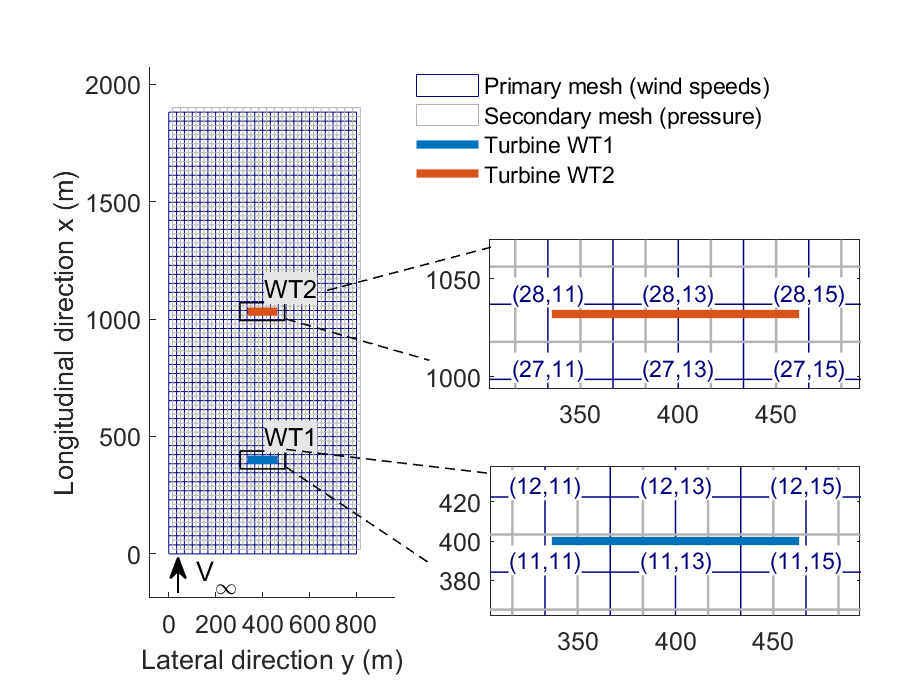
\includegraphics[width=0.65\textwidth]{figures/figures_IFAC23/gridmesh2_tex.eps}
    \caption[WFSim mesh setup for the two-turbine wind farm.]{WFSim mesh setup for the two-turbine wind farm with upstream turbine WT1 (\mlBlue) and downstream turbine WT2 (\mlOrange). The primary mesh (\mlPrimaryMesh) is used for wind speed calculations, and the secondary mesh (\mlSecondaryMesh) for pressure. Zoomed-in areas show primary grid point indices.}
    \label{fig:WFSimMesh2}
\end{figure}
The simulation domain spans~1882\,m in the longitudinal direction and~800\,m in the lateral direction. The primary grid, in blue, is used to compute the longitudinal and lateral wind speeds, and the secondary grid, in gray, is utilized for pressure calculations. Both grids have identical dimensions with a total of 1250 nodes, consisting of 50 nodes in the longitudinal and 25 nodes in the lateral direction. This results in a spatial resolution of $\Delta x = 37.64\,\mathrm{m}$ and $\Delta y = 32\,\mathrm{m}$, with a 1:1 ratio between the primary and secondary grids. The grids are shifted so that the corner nodes of the secondary grid coincide with the center of the mesh cells of the primary grid. The upstream turbine WT1 is represented by a blue bar, and the downstream turbine WT2 by a red bar. The areas around the turbines are shown as zoomed-in plots to clarify which grid points are used in the calculation of the effective wind speeds. For WT1, these are five grid points located in the 11$^{\text{th}}$ row in the longitudinal direction, from the 11$^{\text{th}}$ to the 15$^{\text{th}}$ points in the lateral direction. For WT2, positioned downstream of WT1, the corresponding five points lie in the 27$^{\text{th}}$ longitudinal grid row. 

A considerable speed-up of the WFSim closed-loop simulation is achieved by reformulating the MPC objective function as a QP and avoiding unnecessarily re-initializing constant parameters in each call to the controller. This reformulation of the MPC algorithm results in a speed-up of the controller function execution by a factor of roughly 30 from 152.57\,s to 5.04\,s, and a reduction of the overall simulation time by a factor of nearly 7 from 177.2\,s to 26.2\,s, see Appendix~\ref{appendixC} for further details on the runtimes. Notably, the qLMPC algorithm achieves a mean execution time of 4.2\,ms per simulation step, rendering it potentially real-time capable, whereas the original NMPC requires a mean time of 127.14\,ms. The Koopman MPC algorithms discussed in this thesis are based on this QP formulation of the nonlinear MPC. 

Figure~\ref{fig:WFSimFlow}(a) presents the WFSim program structure diagram for a closed-loop simulation of the original nine-turbine setup. Figure~\ref{fig:WFSimFlow}(b) shows the function used for simulation of Koopman MPC schemes for the two-turbine setup presented in this thesis. While the general program flow and underlying NSE calculations of WFSim are preserved, considerable code modifications and enhancements are necessary in the initialization, the model and the MPC part of the code. These functions are highlighted in Figure~\ref{fig:WFSimFlow}(b) and functions introduced for the Koopman MPC are furthermore written in bold letters. The diagrams are generated using the MATLAB profiler during a closed-loop run with the nonlinear MPC controller integrated into WFSim and the Koopman MPC published in \cite{sharan2022Koopman}. The functions are reordered based on their dependencies to visualize the sequence of function calls.
%\begin{figure}[h]
%    \centering
%    \includegraphics[width=0.65\textwidth, trim=0mm 5mm 7mm 0.1mm, clip]{figuresBlockDiagram_IFAC23/FlowchartInitCtrlPlant_1.eps}
%    \caption{WFSim program structure diagram. Initialization, wind farm model, and controller functions are enclosed in black, blue, and red boxes, respectively. The modified functions \textit{Actuator} and \textit{BoundaryConditions} are highlighted in blue.}
%    \label{fig:WFSimFlow}
%\end{figure}
\begin{figure}[ht]
    \centering
    \subfloat[Original program structure]{
        \begin{minipage}[b]{0.495\textwidth}
            \includegraphics[width=\textwidth, trim=0mm 5mm 29.5mm 0.1mm, clip]{figures/figuresBlockDiagram_IFAC23/FlowchartInitCtrlPlant_1.eps}
        \end{minipage}
    } %\hfill 
    \subfloat[Modified program structure]{
        \begin{minipage}[b]{0.495\textwidth}
            \includegraphics[width=\textwidth, trim=0mm 5mm 29.5mm 0.1mm, clip]{figures/figuresBlockDiagram_IFAC23/FlowchartInitCtrlPlant_2.eps}
        \end{minipage}
    }
    \caption[WFSim program structure diagram.]{WFSim program structure diagram. Initialization, wind farm model, and controller functions are enclosed in black, blue, and red boxes, respectively. Modified functions in (b) are highlighted in black, blue, and red within their respective sections, and functions added for Koopman MPC are indicated in bold.}
    \label{fig:WFSimFlow}
\end{figure}
The entry point to the simulation is the script \textit{WFSim\_demo.m}. Prior to the simulation loop, several initialization functions are called to define the environment and controller parameters as shown in Figure~\ref{fig:WFSimFlow}:

\begin{itemize}\item The script initializes the wind farm layout, setting the number of turbines and their positions, using functions with the naming pattern \textit{layoutSet\_sowfa\_...m}. It specifies the thrust and yaw control signals in \textit{controlSet\_sowfa\_...m}. For the open-loop data generation used to derive the Koopman models presented in \cite{sharan2022Koopman} and \cite{dittmer2022data}, custom signal sets are generated. On the other hand, for closed-loop studies, where only the initial control signal value is selected from the provided vectors and all consecutive control decisions are derived with the control algorithm, the existing files are selected for convenience.
    
    \item The simulation path is set via \textit{WFSim\_addpaths.m} and the solver settings are defined in \textit{solverSet\_default.m}. In the modified structure (Figure~\ref{fig:WFSimFlow}b), the path initialization is the first function to be called, as all commands handling the addition of functions to the executable MATLAB path are moved into this function for a cleaner program structure. It is also modified to ensure that all custom Koopman and QP-based functions can be executed.
    
    \item The function \textit{InitWFSim.m} initializes the wind field, while \textit{meshing.m} defines the computational grid and prepares the MATLAB structures for the simulation.
    
    \item The function \textit{Compute\_B1\_B2\_bc.m} computes the boundary conditions $\bm{b}^\mathrm{BC}$ and the associated matrices $B_1$ and $B_2$. The original implementation calls this function only once, resulting in static boundaries. The modified version calls it whenever the freestream wind changes, enabling non-stationary simulation runs \cite{dittmer2022data}.
    
    \item In the modified program flow, two new functions are added to the initialization phase: \textit{MPCinitK.m} and \textit{koopmanstateextensionWFSim.m}. These functions load the state space model containing the finite-dimensional representation of the Koopman operator, which are used for the subsequent MPC execution.
\end{itemize}
The changes to the turbine states, such as thrust and power, and the wind field at each mesh point are calculated within the simulation loop in \textit{WFSim\_timestepping.m}. The function \textit{Make\_Ax\_b.m} is the core of the WFSim simulation, assembling the system matrices through the following subfunctions:

\begin{itemize}\item In \textit{SpatialDiscr\_Hybrid.m}, a hybrid differencing scheme discretizes the convection terms of the NSE on the 2D mesh. It computes the convection coefficients in both the longitudinal and lateral directions, which are essential for solving the discretized fluid flow equations.
    
    \item The function \textit{Dynamical.m} adds the time-dependent terms of the NSE. It updates the discretization coefficients with unsteady contributions and builds the dynamic source terms representing mass and momentum storage effects based on the velocity field from the previous timestep.
    
    \item The function \textit{Actuator.m} models the actuator-disk representation of the wind turbines within the flow solver. It computes the thrust forces, wake deflection, and power extraction for each turbine. It inserts these forces into the momentum equations and updates turbine data, including power $P$, thrust $F_{T,r}$, yaw $\gamma$, and the coefficients $c_P$ and $c_F$. In \cite{dittmer2023koopman}, a lookup table is integrated into this function to dynamically adjust the power and thrust coefficients based on the yaw angle.
    
    \item In \textit{BoundaryConditions.m}, the boundary conditions for the discretized momentum equations are assigned, enforcing zero-gradient outflow and specific inflow conditions. As shown in the modified structure, this function is adapted in \cite{dittmer2022data} to account for a time-varying freestream wind.
    
    \item The function \textit{MakingSparseMatrix.m} creates the sparse matrix representation of the finite-volume discretization. It is called twice, once for the longitudinal and once for the lateral wind speed components, to construct the system matrices $A_x$ and $A_y$.
\end{itemize}
%
Following the matrix assembly, \textit{Computesol.m} solves the resulting system of equations to obtain the current wind speeds and pressure at the nodes as a vectorized solution. Finally, \textit{MapSolution.m} maps this vector back onto the 2D flow field and updates the boundary conditions for the subsequent simulation iteration. Figure~\ref{fig:WFSimFlow} illustrates the program structure diagram of the controller call within the red box, situated below the wind farm model functions (blue box). In the original code (Figure~\ref{fig:WFSimFlow}a), all controller information, including constant parameters, was re-initialized at every timestep using \textit{MPCinit.m}. In the versions developed in \cite{sharan2022Koopman}, \cite{dittmer2022data}, and \cite{dittmer2023koopman}, only the wind-dependent input matrices are updated, while all constant values are established during the initial setup. In the original implementation, the MATLAB-based modeling framework YALMIP \cite{lofberg2004yalmip} is then initialized to parse the optimization problem. 
%
The thrust commands $C^{\prime}_T$ are calculated in the \textit{NMPCcontroller.m} function through three steps, while the yaw angles $\gamma$ are set to zero:
\begin{itemize}
    \item In \textit{wfmodel.m}, the wind turbine matrices are used to form the wind farm system and input matrices, which are block-diagonal matrices with the turbine matrices on their diagonal.
    \item Based on these, \textit{matsys.m} builds the prediction matrices over the horizon.
    \item The optimal control signals are obtained by solving the resulting MPC problem via the YALMIP function \textit{optimize.m}, with CPLEX as the solver.
\end{itemize}
%
In the modified structure (Figure~\ref{fig:WFSimFlow}b), this workflow is replaced by the \textit{qLPVMPCcontroller\_dU\_\allowbreak quadprog.m} function. This new controller utilizes matrices initialized in \textit{koopmanstateextensionWFSim.m} and initializes wind-dependent input matrices from \textit{MPCinit\_ctrl.m}. The functions \textit{wfmodel.m} and \textit{matsys.m} are modified to accommodate these changes and to construct the parameter-dependent Toeplitz-like matrices and boundary conditions for the QP formulation. These are passed to \textit{quadprog\_sol.m}, which calls the MATLAB solver \textit{quadprog.m}. While the original implementation performed two iterations to refine wind speed predictions, no clear benefit regarding tracking error minimization was observed in the studies forming the basis of this thesis when running the optimization twice. The loop with two iterations is retained in the code. However, as the predicted effective wind speeds do not depend on the decision variables, the second iteration yields the same solution as the first one, so that effectively the farm control signal is calculated only once at each sample.

The following section outlines the calculation of the wind field using the signals $C^{\prime}_T$ and $\gamma$ from \textit{Actuator.m}, the matrices $A_x$ and $A_y$ from \textit{MakingSparseMatrix.m}, and the boundary terms $B_1$, $B_2$, and $\bm{b}^\mathrm{BC}$ from \textit{Compute\_B1\_B2\_bc.m}.

\subsection{Physical Modeling Concepts in WFSim}
In WFSim, wake effects on air pressure and wind speed are modeled using the 2D NSE, which are defined in Equation~\eqref{eq:NSE2d} in Section~\ref{Subsection:WindFarmSimulationModels} and implemented in \textit{Make\_Ax\_b.m} and its subfunctions. For clarity, the NSE are restated here to directly link the physical concepts to their numerical implementation:  
\begin{align*} 
    \frac{\partial \bm{v}}{\partial t}+ (\bm{v}\cdot \nabla_H)\bm{v} + \nabla_H p + \nabla_H\cdot\bm{\tau}_h  - \bm{f} = \bm{0}_{2\times1},\quad  
    \nabla_H\cdot \bm{v} =  -\frac{\partial v_y}{\partial y}
\end{align*}
where $\bm{v} =[v_x\;\;v_y]^T$ consists of the wind components in the $x$- and $y$-directions, respectively. The horizontal gradient operator is $\nabla_H =[\partial/\partial x \;\; \partial/\partial y]^T$, and $p = p(x,y,z_h)$ is the normalized pressure at hub height $z_h$, scaled by air density $\rho_a$. The subgrid stress tensor for horizontal turbulence is denoted by $\bm{\tau}_h$, and $\bm{f}$ represents the turbine-induced forces acting on the flow. These terms are detailed in Section~\ref{Subsection:WindFarmSimulationModels}, which provides the physical background for the wind farm models.

The resulting two-dimensional aerodynamic force vector $\bm{f}_n$, which is applied to the flow field by turbine $n$, is calculated as:
\begin{align}\label{eq:forceNdim2}
    \bm{f}_n =  
    \begin{bmatrix}
        f_{x,n} \\
        f_{y,n}
    \end{bmatrix} 
    = \frac{1}{2} c_f C_{Tn}' \left(V_n \cos(\gamma_n)\right)^2
    \begin{bmatrix}
        \cos(\gamma_n + \phi) \\
        \sin(\gamma_n + \phi)
    \end{bmatrix} \in \mathbb{R}^{2\times 1},
\end{align}
where $C_{Tn}^{\prime}$ is the thrust control signal of turbine $n$ used to regulate axial induction. The variable $\gamma_n$ is the turbine yaw angle, and $\phi$ is the inflow wind direction. The scalar $V_n$ represents the magnitude of the effective wind speed at the rotor center of turbine $n$, and $c_f$ (kg/m) is a model calibration constant used to scale the applied thrust to match high-fidelity simulation or measurement data.

For the numerical implementation, the domain is discretized into an $n_p = n_x \cdot n_y$ grid of pressure cells. WFSim utilizes a staggered grid configuration: the longitudinal wind speed $v_x$ is stored on horizontal cell edges (normal to the vertical x-axis), and the lateral wind speed $v_y$ is stored on the vertical cell edges (normal to the horizontal y-axis). Note that in the WFSim matrix convention, the $x$-axis corresponds to the row index, i.e., the longitudinal direction, and the $y$-axis to the column index, the lateral direction.

This discretization yields $n_{v_x} = n_x \cdot (n_y+1)$ unknowns for the longitudinal velocity and $n_{v_y} = (n_x+1) \cdot n_y$ unknowns for the lateral velocity. Therefore, the 2D force components from Equation~\eqref{eq:forceNdim2} are mapped to the grid and assembled into the vector $\bm{f}$:
\begin{align}\label{eq:forceWFSim}
    \bm{f}_n \;\mapsto\; \bm{f} =
    \begin{bmatrix}
        \bm{f}_{x} \\[1mm]
        \bm{f}_{y}
    \end{bmatrix} \in \mathbb{R}^{(n_{v_x}+n_{v_y}) \times 1}, 
    \qquad 
    \bm{f}_{x} \in \mathbb{R}^{n_{v_x} \times 1}, \quad
    \bm{f}_{y} \in \mathbb{R}^{n_{v_y} \times 1}.
\end{align}
For the example utilized in this thesis, with $n_x = 50$ and $n_y = 25$, the dimensions are:
\begin{align*}
    n_{v_x} = 1300,\;  n_{v_y} = 1275, \;\text{and}\; n_{p} = 1250,
\end{align*}
which results in a total state dimension of $n_q = n_{v_x} + n_{v_y} + n_p = 3825$.

After spatial and temporal discretization, the system dynamics are described by the following difference equation:
\begin{align} \label{eq:WfsinGrid}
    E(q_k)q_{k+1} = Aq_k + \bm{b}(q_k, w_k)
\end{align}
where the system state vector $q_k \in \mathbb{R}^{\,n_q}$ contains the wind speed components and pressure at sample time $k$:
\[
q_k = 
\begin{bmatrix} 
    \bm{v}_x^T   & \bm{v}_y^T   & p^T   
\end{bmatrix}^T \in \mathbb{R}^{\,n_{q} \times 1}.
\]
The control input vector is defined as:
\[
w_k = 
\begin{bmatrix} 
    (\bm{C}_{T,k}^{\prime})^T   & \bm{\gamma}_k^T   
\end{bmatrix}^T   
\in \mathbb{R}^{\,2n_{\mathrm{WT}}\times 1},
\]
where $\bm{C}_{T,k}^{\prime}, \bm{\gamma}_k \in \mathbb{R}^{\,n_{\mathrm{WT}}}$ correspond to the thrust control signals and yaw angles of the $n_{\mathrm{WT}}$ turbines.

The matrices $E(q_k) \in \mathbb{R}^{\,n_{q} \times n_{q}}$ and $A \in \mathbb{R}^{\,n_{q} \times n_{q}}$ describe the interaction between the interior grid points, while $\bm{b}$ is the forcing vector combining boundary conditions and control inputs. Specifically, $E(q_k)$ and  $A$ are structured as
\begin{align} \label{eq:AGrid}
    E(q_k) =
    \begin{bmatrix}
        A_x(\bm{v_{x,k}},\bm{v_{y,k}}) & 0   & B_1 \\
        0   & A_y(\bm{v_{x,k}},\bm{v_{y,k}}) & B_2 \\
        B_1^T   & (2 B_2)^T   & 0
    \end{bmatrix} \text{ and } 
    A =
    \begin{bmatrix}
        A_{11} & 0   & 0 \\
        0   & A_{22} &0 \\
        0   & 0   & 0
    \end{bmatrix},
\end{align}
where $A_x \in \mathbb{R}^{\,n_{v_x} \times n_{v_x}}$ and $A_y \in \mathbb{R}^{\,n_{v_y} \times n_{v_y}}$ are the sparse discretization matrices for the longitudinal and lateral momentum equations.  The matrices $B_1 \in \mathbb{R}^{\,n_{v_x} \times n_p}$ and $B_2 \in \mathbb{R}^{\,n_{v_y} \times n_p}$ couple the pressure field to the momentum equations, while $B_1^T$ and $(2 B_2)^T$ represent the discrete continuity equation acting on the pressure term. The factor of 2 in the $(2B_2)^T$ term arises from a modeling heuristic used to approximate 3D flow effects within a 2D framework. By assuming the vertical flow divergence $\partial w / \partial z$ is approximately equal to the lateral divergence $\partial v / \partial y$, the continuity equation is modified to $\partial u / \partial x + 2\partial v / \partial y = 0$. This adaptation allows the model to simulate mass leakage into the third dimension, preventing the unphysical flow accelerations often seen in standard 2D wake models and providing a better fit to high-fidelity LES data. The diagonal blocks $A_{11} \in \mathbb{R}^{\,n_{v_x} \times n_{v_x}}$ and $A_{22} \in \mathbb{R}^{\,n_{v_y} \times n_{v_y}}$ describe the influence of the longitudinal and lateral velocities at the current time step on those in the next sample.

The forcing vector $\bm{b}(q_k, w_k) \in \mathbb{R}^{n_q\times 1}$ in Equation~\eqref{eq:WfsinGrid} is defined as:
\begin{align} \label{eq:bGrid}\bm{b}(q_k, w_k) =\begin{bmatrix}\bm{f}_x(q_k, w_k) + \bm{b}_x^\mathrm{BC} \\ \bm{f}_y(q_k, w_k) + \bm{b}_y^\mathrm{BC} \\ \bm{0}\end{bmatrix},\end{align}
where $\bm{f}_x$ and $\bm{f}_y$ are the discrete aerodynamic force contributions from the turbines—calculated via the actuator disk model—and $\bm{b}_x^\mathrm{BC}, \bm{b}_y^\mathrm{BC}$ represent the contributions from the velocity boundary conditions. The zero block corresponds to the continuity equation, which remains unforced as it represents the mass conservation constraint. Thus, $\bm{b}(q_k, w_k)$ encompasses all external inputs and boundary constraints driving the state evolution. Although the system state dimension $n_q$ is large, even for the two-turbine case, the matrices are highly sparse and structured due to the finite-volume discretization on the staggered grid. This sparsity allows Equation~\eqref{eq:WfsinGrid} to be solved efficiently using sparse linear algebra techniques.

In the following subsection, the specific wind farm layout and simulation parameters utilized for the studies in this thesis are detailed.
\subsection{WFSim Simulation Setup and Wind Farm Layout}
The simulation studies presented in this thesis, the adaptive AIC \cite{dittmer2022data} and the WRC-AIC \cite{dittmer2023koopman}, utilize an identical wind farm layout. This setup corresponds to the default two-turbine configuration in WFSim, which is also employed in the earlier study \cite{sharan2022Koopman}. The simulation parameters are summarized in Table~\ref{table:WfSim}. 
%
\begin{table}[ht]
    \centering
    \caption{WFSim simulation parameters for the two NREL 5MW turbine setup.}
    \label{table:WfSim}
    \begin{tabular}{l l l l} 
        \toprule
        Description & Symbol & Value & Unit\\
        \midrule
        Domain size &$L_x\times L_y$ & $1882\times 800$& $\text{m}^2$ \\
        Grid size  &$n_x\times n_y$ & $50\times 25$ & -\\
        Number of turbines& $n_{\text{WT}}$ & 2 & - \\
        Rotor diameter & $D$  & $126.4$& m \\
        Turbine spacing & $5D$ & 632 & m\\
        Sample time &$\Delta t$ & $1$ & s \\
        Longitudinal freestream wind &$v_{x,\infty}$&  $7 - 9$ & m/s \\
        Lateral freestream wind &$v_{y,\infty}$  & $0$ & m/s \\         
        Thrust controls & $C^{\prime}_{T,\text{min}}$, $C^{\prime}_{T,\text{max}}$ & 0.2, 2 & -\\
        Yaw angles &$\gamma_1$, $\gamma_2$ &  $0 - 22$, $0$ & deg\\
        \bottomrule
    \end{tabular}
\end{table}
%
The turbines are modeled after the NREL 5MW turbine, featuring a rotor diameter of $D = 126.4\,\text{m}$. They are spaced~$632\,\text{m}$ apart, corresponding to a streamwise distance of five rotor diameters downstream~($5D$). The discrete simulation sample time is set to $1\,\text{s}$. Regarding wind conditions, the lateral freestream component is set to $0\,\text{m/s}$ for both studies. However, the longitudinal freestream wind speed $v_{x,\infty}$ differs: in the adaptive AIC study \cite{dittmer2022data}, it varies between $7\,\text{m/s}$ and $9\,\text{m/s}$, whereas in the WRC-AIC study \cite{dittmer2023koopman}, it is held constant at $8\,\text{m/s}$.

The thrust control inputs $C_T'$ are constrained within the range $[0.2, 2]$.  Both turbines face the wind directly ($\gamma = 0^{\circ}$) in the AIC algorithm. In the WRC-AIC application, the upstream turbine is permitted a maximum yaw misalignment of $22^{\circ}$.

With this simulation setup and the code modifications described in Section~\ref{sec:WFSim Program Structure and Code Modifications}, the adaptive qLMPC algorithm can be applied to the wind farm. The following section discusses the design and implementation of the AIC algorithm.

\section{Adaptive Wind Farm qLMPC with Thrust Control} \label{sec:AdaptiveWindFarmqLMPCforAIC}
Accurately describing the complex turbulence evolution caused by wakes using closed-form low-order ODEs is infeasible. Therefore, the standard MPC controller available in the open-source WFSim environment explicitly models only the turbine dynamics. Wake interactions are accounted for implicitly by utilizing the effective wind speeds at the turbines as inputs to the model. This architecture is illustrated in the block diagram in Figure~\ref{figBlockDiagramFarm}, presented in Section~\ref{Subsection:Windfarmcontrol}, which provides an overview of the WFSim MPC framework.

In this section, an MPC design is presented that does not require measurements of these effective wind speeds and that adapts its model online to learn dynamics that were not present in the initial training data. The data generation process for open-loop training and closed-loop controller testing is described. This is followed by a discussion of the data handling procedures required to derive an Extended Dynamic Mode Decomposition (EDMD) model, along with a review of the resulting wind farm model and the MPC algorithm itself. Finally, simulation results for both open-loop wind estimation and closed-loop adaptive control are presented. 

\subsection{Simulation Setup for Thrust Control}
Figure~\ref{fig:WFSimFlowAIC} visualizes the data flow of the qLMPC scheme for the two-turbine wind farm. The upstream turbine is denoted WT1 and the downstream turbine WT2. A  distinction from the original WFSim implementation is that the effective wind speeds of the turbines are not fed back directly to the controller. Instead, their trajectories over the prediction horizon are predicted using the EDMD-based model introduced in~\cite{sharan2022Koopman}, and the current effective wind speeds, which initialize these predictions, are estimated from the measured turbine powers, see Equation~\eqref{eq:VrFromPower} below. While the freestream wind speed was held constant in that study, in \cite{dittmer2022data} the longitudinal component $V_\infty = v_{x,\infty}$ is varied, while the lateral component $v_{y,\infty}$ remains zero.
%
\begin{figure}[htp]
    \centering
    \includegraphics[width=1\textwidth,trim={0 0cm 0cm 0.3cm},clip]{figures/figuresBlockDiagram_IFAC23/farmCtrl16_P_multVthesis_EDMD.pdf}
    \caption[Block diagram of WFSim for AIC]{Block diagram of WFSim for AIC with farm control input signals $P_{\text{ref}}$, $P_1$, $P_2$, thrust control signals $C_{T1}^{\prime}$ and $C_{T2}^{\prime}$, freestream wind $V_\infty$ and wind $V_1 = V_{1_m}$. Wind speeds directly in front and behind the $i$-th turbine are $V_{i_1}$ to $V_{i_{n_r}}$ and $V_{i\text{out}_1}$ to $V_{i\text{out}_{n_r}}$. The input to the EDMD model (\mlOldBlue) are $C_{T1}^{\prime}$ and $C_{T2}^{\prime}$, its output are the effective wind speeds $V_{r1}$ and $V_{r2}$.}
    \label{fig:WFSimFlowAIC}
\end{figure}
%
The visualization in Figure~\ref{fig:WFSimFlowAIC} is adapted from the general WFSim diagram (Figure~\ref{figBlockDiagramFarm}) to explicitly distinguish between the local wind speed $V_{1_m}$ and the effective wind speed $V_{r1}$. To achieve this without overcrowding the diagram, the following modifications regarding signals and their visual representation as arrows are made:
\begin{itemize}
    \item In contrast to Figure~\ref{figBlockDiagramFarm}, where local wind speeds were summarized into vectors denoted $\bm{V}_{o1}$ and $\bm{V}_{o2}$, Figure~\ref{fig:WFSimFlowAIC} explicitly displays the individual wind speed signals $V_{1\text{out}_1}$ to $V_{1\text{out}_{n_r}}$ behind WT1. This visualization highlights the spatial signals involved in the wake interaction, while the corresponding signals behind WT2 are omitted, as they do not contribute to the MPC algorithm. Similarly to the rotor outflow, the rotor inflow velocities $V_{1_1}$ to $V_{1_{n_r}}$ and  $V_{2_1}$ to $V_{2_{n_r}}$ are visualized as arrows in Figure~\ref{fig:WFSimFlowAIC}.
    \item The turbine forces resulting from the effective wind speeds and control inputs are calculated within the standard WFSim MPC and are retained as states in the turbine model, see Equation~\eqref{eqPowerWT} in Chapter~\ref{Subsection:Windfarmcontrol} or Equation~\eqref{eqPowerWTAIC_vector}. However, since they are not used in the cost function of either MPC scheme and do not affect the control inputs, they are omitted from Figure~\ref{fig:WFSimFlowAIC} to reduce visual clutter.
\end{itemize}
%
The signals depicted in Figure~\ref{fig:WFSimFlowAIC} are:
\begin{itemize}
    \item Freestream wind $V_\infty$: the freestream wind condition, consisting of a varying longitudinal component $v_{x,\infty}$ and a zero lateral component.
    \item Farm power reference $P_{\text{ref}}$: the reference power output for the entire wind farm.
    \item Wind $V_1$: the local wind speed at the rotor center of the upstream turbine (labeled $V_{1_m}$ in the figure). It is not used by the controllers in this thesis.
    \item Rotor inflow $V_{1_1}$ to $V_{1_{n_r}}$: the array of local wind speeds at the $n_r$ grid points directly in front of the rotor of WT1.
    \item Effective wind $V_{r1}$: the mean of the inflow velocities $V_{1_1}$ to $V_{1_{n_r}}$ acting on WT1. In closed loop, it is estimated from $P_1$ with Equation~\eqref{eq:VrFromPower}.
    \item Control signal $C_{T1}^{\prime}$: the thrust control signal applied to WT1.
    \item Power $P_1$: the electrical power generated by WT1.
    \item Rotor outflow $V_{1\text{out}_1}$ to $V_{1\text{out}_{n_r}}$: the local wind speeds at the grid points directly behind WT1.
    \item Rotor inflow $V_{2_1}$ to $V_{2_{n_r}}$: the array of local wind speeds directly in front of the rotor of WT2, which are affected by the wake of WT1.
    \item Effective wind $V_{r2}$: the mean of the inflow velocities $V_{2_1}$ to $V_{2_{n_r}}$ acting on WT2.
    \item Control $C_{T2}^{\prime}$: the thrust control signal applied to WT2.
    \item Power $P_2$: the electrical power generated by WT2.
\end{itemize}
Specific signals from this set are recorded during open-loop simulations to construct the linear EDMD models. The identified model utilizes  the thrust control signals $C_{T1}^{\prime}$ and $C_{T2}^{\prime}$, to estimate two outputs, the effective wind speeds $V_{r1}$ and $V_{r2}$.


Given that the yaw angle of both turbines is fixed at $0^\circ$ for the AIC algorithm, the effective wind speed of Equation~\eqref{eqEffWindSpdWT}, i.e., the mean of the wind speed components normal to the rotor, reduces to the mean of the longitudinal wind speed components:
\begin{align} \label{eqEffWindSpdWTAIC}
    V_{ri} &=  \frac{1}{n_r} \sum_{j = 1}^{n_r} V_{i_j},  
    \quad  V_{i_j} = \cos(\phi_{i_j}) \sqrt{v_{x,i_j}^2 + v_{y,i_j}^2} = v_{x,i_j},
    \quad \phi_{i_j} = \arctan\left(\frac{v_{y,i_j}}{v_{x,i_j}}\right),
\end{align}
where $v_{x,i_j}$ and $v_{y,i_j}$ represent the wind speed components in the $x$- and $y$-direction at the $j$-th of $n_r$ mesh points in front of the $i$-th turbine rotor.

In the closed-loop simulations of this thesis, the controllers do not use the effective wind speeds of Equation~\eqref{eqEffWindSpdWTAIC}, which would require measuring the inflow over the rotor. Instead, the effective wind speeds are estimated from the measured powers $P_i$ by inverting the power model of the actuator disk in WFSim:

\begin{align} \label{eq:VrFromPower}
    \tilde{V}_{ri} = \left( \frac{P_i}{c_{P,i}(\gamma_i)\, \tfrac{1}{2}\rho_a A_r \, C_{Ti}^\prime} \right)^{1/3},
\end{align}
where $c_{P,i}(\gamma_i)$ is the power scaling factor of WFSim including the yaw-dependent lookup table described in Section~\ref{sec:WindFarmSimulationWFSim}, so that the same estimate is used for the AIC and the WRC-AIC. Since WFSim computes the power from the mean of the cubed wind speeds over the rotor, $\tilde{V}_{ri}$ is the cubic mean of the rotor inflow. For the AIC with zero yaw, it deviates from the effective wind speed by at most 0.003\,m/s; for the WRC-AIC with yaw misalignment and a partially waked downstream rotor, it is on average 0.02\,m/s, i.e., 0.3\%, larger. The effect on the closed-loop results is discussed in Sections~\ref{section:AICWindFarmControl} and~\ref{SimResults}.


\subsection{Koopman-Based Identification of qLPV Models}
To derive a Koopman-based linear model for predicting the effective wind speeds, open-loop simulations are first performed to generate training data. Before applying EDMD, this data is lifted using nonlinear functions, following the fundamental principles of Koopman operator theory. This section summarizes the model identification procedure using EDMD and its adaptation for data-driven adaptive control. While the Koopman operator and its matrix representation are described in detail in Sections~\ref{KoopmanOperator} and~\ref{KoopmanIdentification},  concepts are revisited here to establish the connection to the qLPV model utilized in the wind farm MPC algorithm.

\subsubsection{Koopman Matrix Creation}

Consider a linear system in the lifted space of the form:
\begin{align}
    \bm{\varphi}(k+1) &= \bm{A} \bm{\varphi}(k) + \bm{B} \bm{w}(k), 
    \quad \hat{\bm{x}}(k) = \bm{C} \bm{\varphi}(k), 
    \label{eq:linearPredictor}
\end{align}
where $\bm{\varphi} \in \mathbb{R}^{n_\varphi \times 1}$ is the lifted state vector containing $n_\varphi$ lifted states, and $\bm{w} \in \mathbb{R}^{n_w \times 1}$ denotes the input vector, which may include both control signals and measured disturbances. The vector $\hat{\bm{x}} \in \mathbb{R}^{n_x \times 1}$ represents the predicted output. The system dynamics are defined by the state matrix $\bm{A} \in \mathbb{R}^{n_\varphi \times n_\varphi}$, the input matrix $\bm{B} \in \mathbb{R}^{n_\varphi \times n_w}$, and the output matrix $\bm{C} \in \mathbb{R}^{n_x \times n_\varphi}$. The initial lifted state is given by $\bm{\varphi}(\bm{x}_0) = [g_{1}(\bm{x}_0)\;\; g_{2}(\bm{x}_0) \;\; \ldots\;\;g_{n_\varphi}(\bm{x}_0)]^T$.

In the proposed framework, the lifted state vector $\bm{\varphi}$ is structured such that its first $n_x$ elements correspond directly to the predicted output $\hat{\bm{x}}$, which are the effective wind speeds, followed by their quadratic and cubic terms:
\begin{align*}
    \bm{\varphi} &= [V_{r1} \quad V_{r2} \quad V^2_{r1} \quad V^2_{r2} \quad  V^3_{r1} \quad V^3_{r2}]^T   \in \mathbb{R}^{n_\varphi \times 1}, \\
    \hat{\bm{x}} &=  [V_{r1} \quad V_{r2}] ^T   \in \mathbb{R}^{n_x \times 1},
\end{align*}
with dimensions $n_\varphi = 6$ and $n_x = 2$. The input vector $\bm{w}$ used in this thesis consists of the thrust control signals of the two wind turbines in the wind farm:
\begin{align} \label{eq:wOnlyCt}
    \bm{w} = \bm{u}_{\text{WF}} = [C^{\prime}_{T1} \quad C^{\prime}_{T2}]^T \in \mathbb{R}^{n_w \times 1},
\end{align}
with $n_w = n_u = 2$, as in \cite{sharan2022Koopman}. In \cite{dittmer2022data}, the input vector additionally contained the measured wind speed in front of the upstream turbine. With an improved selection of the identification signals, the models identified without this input reach an acceptable performance level, see the discussion of simulation results in Section~\ref{section:AICWindFarmControl}. This removes the need to measure the freestream wind upstream of the wind farm; the effective wind speeds at the turbines, which initialize the lifted state, are still required; in this thesis, they are estimated from the measured turbine powers with Equation~\eqref{eq:VrFromPower}. Changes of the freestream wind are then captured by the online model update rather than by a disturbance input.

EDMD is employed to calculate the Koopman matrix, which approximates the infinite-dimensional Koopman operator $\mathcal{K}$ \cite{arbabi2018data}. To facilitate this, the extended lifted states, which combine the nonlinear state lifted states and the inputs, are defined as:
\begin{align}\label{eq:extLiftObs}
    \bm{\varphi}_w(\bm{x},\bm{w}) = 
    \begin{bmatrix}
        \bm{ \varphi}\\ \bm{w}
    \end{bmatrix} \in \mathbb{R}^{(n_\varphi + n_w) \times 1}.
\end{align}
For the considered setup, this results in a total dimension of $n_\varphi + n_w = 8$. Here, $\bm{\varphi} = \bm{g}(\bm{x}) \in \mathbb{R}^{n_\varphi \times 1}$ denotes the vector of nonlinear state lifted states, and $\bm{w} \in \mathbb{R}^{n_w \times 1}$ is the input vector, which appears linearly in the lifted dynamics.

Given $n_o$ samples of state and input data collected in simulation runs, the data snapshot matrices are defined:
\begin{align} \label{eq:DataCollAIC}
    \bm{X} &= \bigl[ [\bm{x}(k)^T \quad \bm{w}(k)^T]^T \bigr]_{k=1}^{n_o-1} \in \mathbb{R}^{(n_x+n_w)\times (n_o-1)}, \\
    \bm{X}_{+} &= \bigl[ [\bm{x}(k+1)^T\quad \bm{w}(k+1)^T]^T \bigr]_{k=1}^{n_o-1} \in \mathbb{R}^{(n_x+n_w)\times (n_o-1)},
\end{align}
where the dimension of the combined state and input vector is $n_x + n_w = 4$. To ensure an accurate approximation of the system dynamics, the number of samples must be significantly larger than the dimension of the extended lifted space ($n_\varphi + n_w$). The data must be sufficiently rich, i.e., excite all relevant frequencies and cover the operating range of interest. For the study presented in \cite{dittmer2022data}, a dataset of $n_o = 32987$ samples, first used in \cite{sharan2022Koopman}, was utilized for identification. While this dataset resulted in satisfying performance for the non-adaptive case at constant wind speed discussed in that earlier study, later investigations showed that for changing wind speeds and an adaptive controller, a newly designed excitation signal exciting a wider range of frequency is beneficial. For the slightly modified study presented here, a dataset of $n_o = 29999$ samples is used. In this dataset, the thrust control signals of both turbines jump independently between random levels in the range 0.5 to 2, each held for 150\,s to 300\,s, i.e., longer than the wake travel time from WT1 to WT2 of roughly 100\,s. Piecewise-constant noise with a standard deviation of 0.05, held for 10\,s, is added, the signals are limited to the range from 0.2 to 2, and their rate is limited to 0.05\,s$^{-1}$. Note that the full thrust signal range of 0.2 to 2 is not used, as the limited range of 0.5 to 2 was found to be sufficient for the selected closed-loop test. If other test cases are added, a training set covering the whole range could be designed. The model for the estimation of the effective wind speeds used in the AIC model is identified from the second sample onwards, so that the start-up of the wake, which also occurs at the beginning of the closed-loop simulations, is included in the data. The farm power prediction model, discussed in Section~\ref{sec:WindFarmLinearMPCforWRC-AIC} is identified from sample 240 onwards, i.e., after 240\,s at the sampling time of 1\,s, when the initial wake development has settled. This start-up phase, which also occurs at the beginning of the closed-loop simulations, is thus excluded from the identification data of the power prediction.

The extended Koopman matrix $\tilde{\bm{K}}$ is obtained by solving the least-squares problem:
\begin{align}
    \min_{\tilde{\bm{K}}} \sum_{k=1}^{n_o-1} 
    \left\|  
    \begin{bmatrix} 
        \bm{g}(\bm{x}(k+1)) \\[1mm] 
        \bm{w}(k+1) 
    \end{bmatrix}   
    - \tilde{\bm{K}} 
    \begin{bmatrix} 
        \bm{g}(\bm{x}(k)) \\[1mm]
        \bm{w}(k) 
    \end{bmatrix} \right\|_2^2.
    \label{eq:ExtendedKoopmanMinimizationProblem}
\end{align}
This matrix possesses the block structure:
\begin{align}
    \tilde{\bm{K}} = \begin{bmatrix} 
        \bm{A}_{\hat{K}} & \bm{B}_{\hat{K}} \\ 
        \bm{A}_{w,\hat{K}} & \bm{B}_{w,\hat{K}} 
    \end{bmatrix},
\end{align}
where 
$\bm{A}_{\hat{K}} \in \mathbb{R}^{n_\varphi \times n_\varphi}$, 
$\bm{B}_{\hat{K}} \in \mathbb{R}^{n_\varphi \times n_w}$, 
$\bm{A}_{w,\hat{K}} \in \mathbb{R}^{n_w \times n_\varphi}$, 
and $\bm{B}_{w,\hat{K}} \in \mathbb{R}^{n_w \times n_w}$.

For controller design, only the system and input matrices $\bm{A}_{\hat{K}}$ and $\bm{B}_{\hat{K}}$ are required. Thus, problem~\eqref{eq:ExtendedKoopmanMinimizationProblem} simplifies to:
\begin{align}
    \min_{\bm{A}_{\hat{K}}, \bm{B}_{\hat{K}}} 
    \sum_{k=1}^{n_o-1} 
    \left\| \bm{g}(\bm{x}(k+1)) - \bm{A}_{\hat{K}} \bm{g}(\bm{x}(k)) - \bm{B}_{\hat{K}} \bm{w}(k) \right\|_2^2.
    \label{eq:ApproxKoopman}
\end{align}
%
With the data matrices defined as
\begin{align}\label{eq:G_Gplus_datamatrices}
    \bm{G} &= \bigl[ \bm{g}(\bm{x}(1)) \;\; \cdots \;\; \bm{g}(\bm{x}(n_o-1)) \bigr] \in \mathbb{R}^{n_\varphi \times (n_o-1)}, \\
    \bm{G}_{+} &= \bigl[ \bm{g}(\bm{x}(2)) \;\; \cdots \;\; \bm{g}(\bm{x}(n_o)) \bigr] \in \mathbb{R}^{n_\varphi \times (n_o-1)}, \\
    \bm{W} &= \bigl[ \bm{w}(1) \;\; \cdots \;\; \bm{w}(n_o-1) \bigr] \in \mathbb{R}^{n_w \times (n_o-1)},
\end{align}
the optimization problem can be equivalently rewritten in matrix form using the Frobenius norm:
\begin{align}
    \min_{\bm{A}_{\hat{K}}, \bm{B}_{\hat{K}}} 
    \left\| \bm{G}_{+} - \bm{A}_{\hat{K}} \bm{G} - \bm{B}_{\hat{K}} \bm{W} \right\|_F^2.
\end{align}
Defining the combined data matrix of lifted states and inputs as:
\begin{align}
    \bm{G}_w = \begin{bmatrix} \bm{G} \\ \bm{W} \end{bmatrix} \in \mathbb{R}^{(n_\varphi + n_w)\times (n_o-1)},
\end{align}
the analytical least-squares solution is given by:
\begin{align}\label{eq:Koop_G_Gplus_datamatrices}
    \hat{\bm{K}} = \begin{bmatrix} \bm{A}_{\hat{K}} & \bm{B}_{\hat{K}} \end{bmatrix} 
    = \bm{G}_{+}  \bm{G}_w^{\dagger}
    \in \mathbb{R}^{n_\varphi \times (n_\varphi + n_w)},
\end{align}
where ${}^\dagger$ denotes the Moore–Penrose pseudoinverse.  The number of samples $n_o$ is typically, as well as in the discussed simulation cases in this thesis, significantly larger than the number of lifted states, i.e., $n_o \gg n_\varphi + n_w$. Provided that the data are sufficiently rich,  $\bm{G}_w$ has full row rank, and the pseudoinverse can be explicitly computed as:
\begin{align*}
    \bm{G}_w^{\dagger} = \bm{G}_w^T (\bm{G}_w \bm{G}_w^T)^{-1} \in \mathbb{R}^{(n_o-1) \times (n_\varphi + n_w)}.
\end{align*}
Substituting this into Equation~\eqref{eq:Koop_G_Gplus_datamatrices} confirms the dimensions:
\[
\underbrace{\hat{\bm{K}}}_{n_\varphi \times (n_\varphi + n_w)} =
\underbrace{\bm{G}_{+}}_{n_\varphi \times (n_o-1)} \cdot
\underbrace{\bm{G}_w^T}_{(n_o-1) \times (n_\varphi + n_w)} \cdot
\underbrace{(\bm{G}_w \bm{G}_w^T)^{-1}}_{(n_\varphi + n_w) \times (n_\varphi + n_w)}.
\]
Equivalently, the identified matrix can be written as $\hat{\bm{K}}_0 = \mathbf{L}_0\,\mathbf{L}_{u,0}^{-1}$ with the initial auto- and cross-correlation matrices
\begin{align*}
    \mathbf{L}_{u,0} = \bm{G}_w \bm{G}_w^T, \quad \mathbf{L}_0 = \bm{G}_{+} \bm{G}_w^T,
\end{align*}
which serve as initial values for the online update explained below.
%
To utilize the identified matrix $\hat{\bm{K}}$ for linear model predictive control, it is partitioned into the system matrix $\bm{A}_{\hat{K}} \in \mathbb{R}^{n_\varphi \times n_\varphi}$ and the input matrix $\bm{B}_{\hat{K}} \in \mathbb{R}^{n_\varphi \times n_w}$. The system matrix consist of the first $n_\varphi$ columns of $\hat{\bm{K}}$, the input matrix of the remaining  $n_w$ columns, see Equation~\eqref{eq:Koop_G_Gplus_datamatrices}.

In \cite{dittmer2022data}, the measured disturbance $V_1$ is part of the input vector, i.e., $n_w = 3$, and needs to be accounted for as an autonomous state within the prediction horizon. In this case, the input matrix is further split into $\bm{B}_{\hat{K},d} \in \mathbb{R}^{n_\varphi \times n_d}$ for the $n_d$ disturbances and $\bm{B}_{\hat{K},u} \in \mathbb{R}^{n_\varphi \times (n_w-n_d)}$ for the control inputs $[C'_{T1} \;\; C'_{T2}]^T$. The final augmented Koopman matrix $\hat{\bm{K}}_{\text{aug}}$ is then constructed to include the disturbance dynamics. Assuming the disturbance remains constant over the prediction horizon, the augmentation is performed as follows:
\begin{align}\label{eq:AugmentedKoopmanMPC}
    \hat{\bm{K}}_{\text{aug}} = \left[\begin{array}{cc|c}
        \bm{A}_{\hat{K}} & \bm{B}_{\hat{K},d} & \bm{B}_{\hat{K},u}\\
        \bm{0}_{n_d \times n_\varphi} & \bm{I}_{n_d} & \bm{0}_{n_d \times (n_w-n_d)}
    \end{array}\right] \in \mathbb{R}^{(n_\varphi+n_d) \times (n_\varphi+n_w)},
\end{align}
where the second block row ensures the persistence of the measured wind speed disturbance throughout the prediction, with $n_d = 1$ in this case. This structure allows the MPC to treat the disturbance as a known, constant state during the optimization of the control sequence. If the vector $\bm{w}$ consists only of control inputs, see Equation~\eqref{eq:wOnlyCt}, then $n_d = 0$ and hence $\hat{\bm{K}}_{\text{aug}} = \hat{\bm{K}}$.


\subsubsection{Koopman Matrix Update}\label{subsec:koopmanOnlineUpdate}

The online update strategy employed here is based on the recursive least squares method proposed in \cite{cisneros2020data}. To minimize computational overhead and memory usage, the model is not updated continuously. Instead, an update is triggered only when the deviation between the measured outputs and the model predictions over a window of length $h$ exceeds a defined threshold $\nu$.

Let $\mathcal{X}_{\nu}$ denote the buffer containing the state and input vectors of the last $h+1$ time instants:
\[
\mathcal{X}_{\nu} = \begin{bmatrix} x_{k}^T & w_{k}^T & \dots & x_{k-h}^T & w_{k-h}^T \end{bmatrix} \in \mathbb{R}^{1 \times (n_x + n_w)(h+1)}.
\]
The triggering condition is formulated using the infinity norm, which allows the threshold $\nu$ to be interpreted in physical units independent of the window length $h$:
\begin{equation} \label{eq:add_data}
    \left\|
    \begin{bmatrix}
        x_{k-h+1} - \hat{x}_{k-h+1} \\
        \vdots \\
        x_{k} - \hat{x}_{k}
    \end{bmatrix}
    \right\|_\infty \geq \nu,
\end{equation}
where $\hat{x}_j = \bm{C}\hat{\bm{\varphi}}(j)$ are the estimates of the running estimator, i.e., the predictions of the current model $\hat{\bm{K}}$ propagated from the lifted state of the previous sample with the applied inputs.

When this condition is met, the Koopman matrix is updated using the data matrices $\mathbf{L}_u^+$ and $\mathbf{L}^+$. At initialization, $\mathbf{L}_u$ and $\mathbf{L}$ are the offline correlation matrices defined above. While \cite{cisneros2020data} utilizes only the current measurement, this work incorporates a batch of the last five measurement samples to provide low-pass filtering and reduced sensitivity to noise. The batch data matrices are defined as
\[
z_{k,5} = [z_{k-5} \;\; z_{k-4} \;\; \dots \;\; z_{k-1}] \in \mathbb{R}^{(n_x + n_w)\times 5}, \quad
x_{k,5}^+ = [x_{k-4} \;\; x_{k-3} \;\; \dots \;\; x_{k}] \in \mathbb{R}^{n_x \times 5},
\]
where $x_{k,5}^+$ contains the successor states of the samples in $z_{k,5}$.
The recursive updates are computed as a weighted sum of the existing correlation matrices $\mathbf{L}_u$ and $\mathbf{L}$ and the new data:
\begin{equation} \label{eq:GA_online}
    \begin{split}
        n_{\text{upd}}^+ &= n_{\text{upd}} + 1,\\
        \mathbf{L}_u^+ &= \frac{1}{n_{\text{upd}}^+} \Big( (n_{\text{upd}}^+-1)\mathbf{L}_u + \bm{\varphi}_w(z_{k,5}) \bm{\varphi}_w(z_{k,5})^T \Big),\\
        \mathbf{L}^+ &= \frac{1}{n_{\text{upd}}^+} \Big( (n_{\text{upd}}^+-1)\mathbf{L} + \bm{\varphi}(x_{k,5}^+) \bm{\varphi}_w(z_{k,5})^T \Big).
    \end{split}
\end{equation}
The updated Koopman matrix is then obtained as $\hat{\bm{K}}^+ = \mathbf{L}^+ (\mathbf{L}_u^+)^{-1}$ and partitioned as in Equation~\eqref{eq:Koop_G_Gplus_datamatrices}. In \cite{dittmer2022data}, this is the augmented Koopman matrix which is split up according to Equation~\eqref{eq:AugmentedKoopmanMPC}.
The counter $n_{\text{upd}}$ acts as a weighting factor. In \cite{cisneros2020data}, this counter monotonically increases. In contrast, here the counter $n_{\text{upd}}$ is reset to $1$ whenever the error norm falls below the threshold. This allows the model to adapt to changing dynamics rather than becoming rigid due to a large historical weight. During active updates, the counter is incremented to integrate the new information.

Finally, accurate online identification requires sufficient spectral content in the input. Since standard control signals may not excite all dynamic modes, an excitation signal is added to the control input during consecutive updates, see Section~\ref{section:AICWindFarmControl}.

In the implementation used in this thesis, the window and batch length is $h = 5$ and the threshold is $\nu = 0.15$\,m/s. Only the effective wind speed $V_{r1}$ of the upstream turbine enters the criterion in Equation~\eqref{eq:add_data}: it reacts first to a change of the freestream wind, whereas the estimation error of $V_{r2}$ in the wake is large also at constant freestream wind and would trigger updates that contain no new information. The estimates are those of the running estimator, see Equation~\eqref{eq:add_data}. After each update, the lifted state of the estimator is re-initialized with the current effective wind speeds; without this reset, the free-running estimate diverges after a change of the freestream wind.
%More details on the implementation of this excitation signal are provided in the results section.
%Future improvements may include explicit limits on $n_{\text{upd}}$ and the introduction of forgetting factors to balance recent and historical data, as suggested in \cite{zhang2019online}.
%Based on the theory in \cite{cisneros2020data}, a brief review on online update of koopman model is provided in this section. To avoid the memory management issues, we can only store $G$, $G_+$ and $U$ vectors at time $k$ ToDo: Make clear that Psi might be a matrix not a vector if more than one sample is included. Aso use our formulation  Phi*Phi' and X1 *Phi' where Phi= [x0;u0] 
% To do: Forgetting factors, weights between previous model and new data, 
% 'keep alert', find balance between new information
% add quotes (Zhang, Princeton, adaptive DMD) ,added several samples
% Differences to Pable: P initialized as 1, so offline identified model is used
% P is reset to 1 when no update is necessary (tuning knob -> future work to 
\subsection{qLMPC Design for Thrust Control} 
The aim of wind farm control considered here is accurate tracking of a power reference with minimal changes in the control inputs, as discussed, e.g., in \cite{vali2019adjoint, boersma2019constrained}.
\subsubsection{Model Derivation and Cost Function}
As mentioned in Section~\ref{Subsection:Windfarmcontrol}, the main difference to the NMPC that ships with WFSim is that the effective wind speeds over the prediction horizon are predicted with a data-driven Koopman model instead of being kept constant. This turns the wind farm model into a qLPV model, as its input matrices depend on the predicted effective wind speeds. The Koopman model is identified with EDMD from data acquired in open-loop WFSim simulations. It uses the two thrust control signals $C_{T1}^{\prime}$ and $C_{T2}^{\prime}$ as inputs and the resulting effective wind speeds as states; the wind speed $V_1$ in front of the first turbine, an additional input in \cite{dittmer2022data}, is not used. Before applying EDMD, the data is extended with nonlinear lifting functions, following the Koopman approach discussed in detail in Section~\ref{KoopmanIdentification}.

For the qLMPC design for adaptive AIC, the same discrete-time wind farm model is used as in the original WFSim NMPC algorithm described in Section~\ref{Subsection:Windfarmcontrol} in Equations~\eqref{eqPowerWT} to~\eqref{eqLinWF}. The procedure used to calculate the evolution of the wind farm power over a prediction horizon is repeated here for ease of understanding, with the only difference being that the yaw angle is fixed to zero. The state-space model of the $i$-th turbine, assuming no yaw control or misalignment, is given by:
\begin{align} \label{eqPowerWTAIC_vector}
    \underbrace{
        \begin{bmatrix}
            P_i(k+1) \\[0.8mm]
            F_{T,ri}(k+1) \\[0.8mm]
            \hat{C}_{Ti}^\prime(k+1)
    \end{bmatrix}}_{\bm{x}_{\text{WT},i}(k+1) \in {\mathbb{R}}^{3\times 1}}
    &=
    \underbrace{(1-\tau)\,\bm{I}_{3\times3}}_{\bm{A}_{\text{WT},i} \in {\mathbb{R}}^{3\times 3}}
    \begin{bmatrix}
        P_i(k) \\[0.8mm]
        F_{T,ri}(k) \\[0.8mm]
        \hat{C}_{Ti}^\prime(k)
    \end{bmatrix}
    +
    \underbrace{\tau
        \begin{bmatrix}
            \tfrac{1}{2}\rho_a A_r \hat{V}_{ri}^3 \\[0.8mm]
            \tfrac{1}{2}\rho_a A_r \hat{V}_{ri}^2 \\[0.8mm]
            1
    \end{bmatrix}}_{\bm{B}_{\text{WT},i}(\hat{V}_{ri}) \in {\mathbb{R}}^{3\times 1}} \, C_{Ti}^\prime(k),
\end{align}
where $k$ is the discrete sample time index and the constant $\tau$ is the discrete-time filter coefficient. The coefficient $\tau$ determines the weighting between the current state and the new input at each time step, thereby controlling the response speed of the turbine states. In contrast to the original WFSim NMPC, the input matrix depends on the predicted effective wind speed $\hat{V}_{ri}$.

In the state vector $\bm{x}_{\text{WT},i}$, $P_i$ denotes the power, $F_{T,ri}$ the thrust force of the $i$-th turbine, and $\hat{C}_{Ti}^\prime$ the filtered thrust control signal:
\begin{align*}
    \bm{x}_{\text{WT},i} = [P_i \quad F_{T,ri} \quad \hat{C}_{Ti}^\prime]^T.
\end{align*}
The thrust force $F_{T,ri}$ is retained in the state vector to remain consistent with the original WFSim implementation, in which it is computed as part of the turbine model. However, since $\bm{A}_{\text{WT},i}$ is diagonal, $F_{T,ri}$ does not influence the other states, and it is not penalized in the cost function. It therefore has no effect on the control inputs computed by the MPC.

The individual turbine models are concatenated into a qLPV system with the vector of all predicted effective wind speeds $\hat{\bm{V}}_r$ as the scheduling parameter vector:
\begin{align} \label{eqLinWFAIC}
    \bm{x}_{\text{WF}}(k+1) &= \bm{A}_{\text{WF}} \bm{x}_{\text{WF}}(k) + \bm{B}_{\text{WF}}(\hat{\bm{V}}_r(k)) \, \bm{C}_{T}^\prime(k),\\
    P_{\text{WF}}(k) & = \underbrace{\bm{1}_{1 \times n_{\text{WT}} } \otimes [1 \quad 0 \quad 0]}_{\bm{C}_{\text{WF}} \in {\mathbb{R}}^{1 \times 3n_\text{WT}}} \, \bm{x}_{\text{WF}}(k), \label{eqLinWFAIC2}
\end{align}
where $\bm{A}_{\text{WF}} \in {\mathbb{R}}^{3n_\text{WT} \times 3n_\text{WT}}$ and $\bm{B}_{\text{WF}}(\hat{\bm{V}}_r) \in {\mathbb{R}}^{3n_\text{WT} \times n_\text{WT}}$ are block-diagonal matrices composed of the turbine matrices $\bm{A}_{\text{WT},i}$ and $\bm{B}_{\text{WT},i}(\hat{V}_{ri})$. The wind farm power $P_{\text{WF}}$ is the sum of all individual turbine powers, $P_{\text{WF}} = \sum_{i=1}^{n_{\text{WT}}} P_i$.

The farm-level state vector, the control input vector, and the vector containing the estimated effective wind speeds of all turbines are defined as:
\begin{align*}
    \bm{x}_{\text{WF}} &= [\bm{x}_{\text{WT},1}^T \quad \bm{x}_{\text{WT},2}^T \quad \dots \quad \bm{x}_{\text{WT},n_{\text{WT}}}^T ]^T \in {\mathbb{R}}^{3n_\text{WT} \times 1},\\
    \bm{C}_{T}^\prime &= [C_{T1}^\prime \quad C_{T2}^\prime \quad \dots \quad C_{T n_{\text{WT}}}^\prime ]^T \in {\mathbb{R}}^{n_\text{WT} \times 1},\\
    \hat{\bm{V}}_r &= [\hat{V}_{r1} \quad \hat{V}_{r2} \quad \dots \quad \hat{V}_{r n_\text{WT}}]^T \in {\mathbb{R}}^{n_\text{WT}\times 1}.
\end{align*}
The vector $\hat{\bm{V}}_r$ is the scheduling parameter vector $\bm{\rho}_{\Rho,\text{WF}}$ introduced in Equation~\eqref{eq:rhoWF}. Over the prediction horizon, it forms the scheduling trajectory
\begin{align*}
    \bm{\Rho}_{\Rho} = [ \hat{\bm{V}}_r^T(k) \quad \hat{\bm{V}}_r^T(k+1) \quad \ldots \quad \hat{\bm{V}}_r^T(k+n_h-1)]^T \in \mathbb{R}^{n_{\text{WT}} n_h \times 1}.
\end{align*}
%
These vectors are used in combination with the parameter-dependent Toeplitz-like matrices built from $\bm{A}_{\text{WF}}$, $\bm{B}_{\text{WF}}$, and $\bm{C}_{\text{WF}}$ to predict the farm power trajectory, similarly to the approach discussed in Section~\ref{sec:qLMPCOptimizationAlgo} and Equation~\eqref{eq:nearlyToeplitzMat}.
% \bm{\varphi}_w
The cost function $J(\bm{U})$ is formulated to minimize the tracking error $\bm{E}$ and control increments $\Delta \bm{U}$:
\begin{align} \label{eq:NMPCcostAIC}
    J(\bm{U}) = \underbrace{\bm{E}^T Q \bm{E}}_{J_Q (\bm{U})} + \underbrace{\Delta \bm{U}^T R \Delta \bm{U} }_{J_R ( \bm{U})},
\end{align}
with weighting matrices $Q = q \cdot \bm{I}_{n_h \times n_h}$ and $R = r \cdot \bm{I}_{n_{hu}\times n_{hu}}$. The tracking error trajectory $\bm{E}(k)$ is defined as:
\begin{equation}\label{eq:errortraject}
    \begin{aligned}
        \bm{E}(k) &= \bm{P}_{\text{ref}}(k) - \hat{\bm{P}}_{\text{WF}}(k) \\
        &= [ e(k+1) \quad e(k+2) \quad \dots \quad e(k + n_h) ]^T \in \mathbb{R}^{n_h \times 1},
    \end{aligned}
\end{equation}
where $e = P_{\text{ref}} - \hat{P}_{\text{WF}}$, i.e., the difference between the reference farm-level power $P_{\text{ref}}$ and the predicted power $\hat{P}_{\text{WF}}$. The reference, predicted power, and control trajectories are given by:
\begin{equation} \label{eq:UandDUAIC}
    \begin{aligned}
        \bm{P}_{\text{ref}}(k) &= [ P_{\text{ref}}(k+1) \quad P_{\text{ref}}(k+2) \quad \dots \quad P_{\text{ref}}(k + n_h)]^T \in \mathbb{R}^{n_h \times 1}, \\
        \hat{\bm{P}}_{\text{WF}}(k) &= [ \hat{P}_{\text{WF}}(k+1) \quad \hat{P}_{\text{WF}}(k+2) \quad \dots \quad \hat{P}_{\text{WF}}(k + n_h)]^T \in \mathbb{R}^{n_h \times 1}, \\
        \bm{U}(k) &= [ \bm{C}_T^{\prime T}(k) \quad \bm{C}_T^{\prime T}(k+1) \quad \dots \quad \bm{C}_T^{\prime T}(k+n_h-1) ]^T \in \mathbb{R}^{n_{hu}\times 1},
    \end{aligned}
\end{equation}
with the length of the control trajectory $n_{hu} = n_h n_{\text{WT}}$, as each turbine has a single control input, its thrust coefficient $C'_{Ti}$. The first element $\bm{C}_T^\prime(k)$ of $\bm{U}(k)$ is the input applied at the current sample, which affects the power from sample $k+1$ onward. The reference trajectory $\bm{P}_{\text{ref}}(k)$ is assumed to be known over the prediction horizon. The trajectory of the control increments contains the changes of the thrust control vector between consecutive time steps:
\begin{align} \label{eq:DUAIC}
    \Delta \bm{U}(k) = [ \Delta\bm{C}_T^{\prime T}(k) \quad \Delta\bm{C}_T^{\prime T}(k+1) \quad \dots \quad \Delta\bm{C}_T^{\prime T}(k+n_h-1) ]^T \in \mathbb{R}^{n_{hu}\times 1},
\end{align}
with $\Delta\bm{C}_T^\prime(k) = \bm{C}_T^\prime(k) - \bm{C}_T^\prime(k-1)$, where $\bm{C}_T^\prime(k-1)$ is the input applied at the previous sample. For the two-turbine case with $n_h = 10$, this yields $\bm{E} \in \mathbb{R}^{10\times 1}$ and $\bm{U}, \Delta \bm{U} \in \mathbb{R}^{20\times 1}$. Finally, the constrained optimization problem is stated as:
\begin{align} \label{eq:ObjFunAIC}
    \begin{array}{ll}
        \underset{\bm{U}(k)}{\text{minimize }} & J(\bm{U}(k)) = \bm{E}^T(k) Q \bm{E}(k) + \Delta \bm{U}^T(k) R \Delta \bm{U}(k) = J_Q(\bm{U}) + J_R(\bm{U}) \\[10pt]
        \text{subject to} & \bm{x}_{\text{WF}}(k+j+1) = \bm{A}_{\text{WF}} \bm{x}_{\text{WF}}(k+j) + \bm{B}_{\text{WF}}(\hat{\bm{V}}_r(k+j)) \bm{C}_{T}^\prime(k+j), \\[10pt]
        & \hat{P}_{\text{WF}}(k+j+1) = \bm{C}_{\text{WF}} \bm{x}_{\text{WF}}(k+j+1), \\[10pt]
        & \bm{C}_{T,\text{min}}^\prime \leq \bm{C}_{T}^\prime(k+j) \leq \bm{C}_{T,\text{max}}^\prime, \quad j = 0, \dots, n_h-1,
    \end{array}
\end{align}
with the current turbine states $\bm{x}_{\text{WF}}(k)$ as initial condition and the limits $\bm{C}_{T,\text{min}}^\prime$ and $\bm{C}_{T,\text{max}}^\prime$ of the thrust control signals.

\subsubsection{Power Prediction, Control Increments and Cost Terms for QP Formulation}
Note that the decision variables in the wind farm optimization problem in Equation~\eqref{eq:ObjFunAIC} are the elements of $\bm{U}$, not of $\Delta \bm{U}$. This is a difference to the velocity-based wind turbine qLMPC in Equation~\eqref{eq:ObjFunWT}. There, the underlying state-space model is velocity-based, so both the error term $\bm{e}$ and the control term depend directly on the decision variable increment $\Delta\bm{u}_{\text{Mdl}^\prime}$. Here, for wind farm control, the error term $\bm{E}$ depends on $\bm{U}$, while the control term depends on $\Delta\bm{U}$. To obtain a QP in $\bm{U}$, both terms are therefore expressed in terms of $\bm{U}$, as shown in the following.

The predicted power trajectory follows from the state-space model in Equation~\eqref{eqLinWFAIC}:
\begin{align*}
    %\hat{\bm{P}}_{\text{WF}}(k) = \tilde{L}\, \bm{x}_{\text{WF}}(k) + \tilde{S}(\hat{\bm{V}}_r)\, \bm{U}(k),
    \hat{\bm{P}}_{\text{WF}}(k) = \tilde{L}\, \bm{x}_{\text{WF}}(k) + \tilde{S}(\bm{\Rho}_k)\, \bm{U}(k),
\end{align*}
with the matrices $\tilde{L} \in \mathbb{R}^{n_h \times 3n_{\text{WT}}}$ and $\tilde{S} \in \mathbb{R}^{n_h \times n_{hu}}$:
\begin{equation} \label{eq:ltildeWF}
    \begin{aligned}
        \tilde{L} &=
        \begin{bmatrix}
            \bm{C}_{\text{WF}} \bm{A}_{\text{WF}} \\ \bm{C}_{\text{WF}} \bm{A}_{\text{WF}}^2 \\ \vdots \\ \bm{C}_{\text{WF}} \bm{A}_{\text{WF}}^{n_h}
        \end{bmatrix}, \\
        \tilde{S}(\hat{\bm{V}}_r) &=
        \begin{bmatrix}
            \bm{C}_{\text{WF}} \bm{B}_{\text{WF},0} & \bm{0} & \cdots & \bm{0} \\
            \bm{C}_{\text{WF}} \bm{A}_{\text{WF}} \bm{B}_{\text{WF},0} & \bm{C}_{\text{WF}} \bm{B}_{\text{WF},1} & \cdots & \bm{0} \\
            \vdots & \vdots & \ddots & \vdots \\
            \bm{C}_{\text{WF}} \bm{A}_{\text{WF}}^{n_h-1} \bm{B}_{\text{WF},0} & \bm{C}_{\text{WF}} \bm{A}_{\text{WF}}^{n_h-2} \bm{B}_{\text{WF},1} & \cdots & \bm{C}_{\text{WF}} \bm{B}_{\text{WF},n_h-1}
        \end{bmatrix},
    \end{aligned}
\end{equation}
where $\bm{B}_{\text{WF},j} = \bm{B}_{\text{WF}}(\hat{\bm{V}}_r(k+j))$ is the input matrix evaluated with the predicted effective wind speeds at step $k+j$. Only $\tilde{S}$ depends on the predicted wind speeds, since $\bm{A}_{\text{WF}}$ and $\bm{C}_{\text{WF}}$ are constant. The current state $\bm{x}_{\text{WF}}(k)$ initializes the prediction and is calculated from the state and input at the previous sample $k-1$.

To evaluate the qLPV wind farm model over the prediction horizon, the estimated effective wind speeds $\hat{V}_{ri}(k+j)$, $j = 1, \dots, n_h$, are required. In \cite{dittmer2022data}, they are predicted with the identified Koopman model in its augmented form, see Equation~\eqref{eq:AugmentedKoopmanMPC}. 
The prediction starts from the estimated lifted state $\hat{\bm{\varphi}}(k)\approx \bm{\varphi}(k)$ predicted at the previous time step. After a model update, it is re-initialized with the lifting of the effective wind speeds $\tilde{\bm{V}}_r(k)$ estimated with Equation~\eqref{eq:VrFromPower}. The inputs, i.e., the thrust coefficients $\bm{C}_T^\prime(k-1)$ applied at the previous sample and, formerly, the measured upstream wind speed $V_1(k)$, are held constant over the horizon. As the matrices $\bm{A}_{\hat{K}}$ and $\bm{B}_{\hat{K}}$ are identified without the wind input and from different open-loop data, they differ from those of \cite{dittmer2022data}. With no wind measurement for the prediction of the effective wind speeds and with matrices $\bm{A}_{\hat{K}}$ and $\bm{B}_{\hat{K}}$ as defined in Equation~\eqref{eq:Koop_G_Gplus_datamatrices} the lifted state trajectories are:
\begin{align*}
    \hat{\bm{\varphi}}(k+j) &= \bm{A}_{\hat{K}}\, \hat{\bm{\varphi}}(k+j-1) + \underbrace{\bm{B}_{\hat{K},u}}_{\bm{B}_{\hat{K}}}\, \bm{C}_T^\prime(k-1) + \cancel{\bm{B}_{\hat{K},d}\, V_1(k)}, \\
    \hat{\bm{V}}_r(k+j) &= \bm{C}\, \hat{\bm{\varphi}}(k+j),\end{align*}
Therefore, the trajectory of the extended lifted state depends at each trajectory sample $k+j$ on the effective wind speed at that sample and the control input applied at the previous control step $k-1$:
\begin{align*}    
    \bm{\varphi}_w(k+j) &= \bm{\varphi}_w\big([\hat{\bm{V}}_r^T(k+j) \;\; \bm{C}_T^{\prime T}(k-1) \;\; \cancel{V_1(k)}]^T\big),
\end{align*}

where $\hat{\bm{V}}_r = [\hat{V}_{r1} \;\; \hat{V}_{r2}]^T$ contains the predicted effective wind speeds and $\bm{C} = [\bm{I}_{2} \;\; \bm{0}_{2 \times 4}]$ selects them from the lifted state.   After each prediction step, the lifted states are recomputed from the predicted wind speeds with the lifting functions from Equation~\eqref{eq:extLiftObs}, so that the nonlinear lifted states remain consistent with the predicted states. The predicted effective wind speeds are then inserted into the input matrices $\bm{B}_{\text{WT},i}(\hat{V}_{ri}(k+j))$ of the turbine models in Equation~\eqref{eqPowerWTAIC_vector}, which yields the time-varying matrices $\bm{B}_{\text{WF},j}$ in $\tilde{S}$. The one-step prediction $\hat{\bm{\varphi}}(k+1)$ is stored as the initial lifted state for the next time step. The predicted effective wind speeds are limited to the physically plausible range from 2 to 12\,m/s. Since the predicted wind speeds do not depend on $\bm{U}(k)$, the matrix $\tilde{S}$ is independent of the decision variables.

The control increments are a linear function of the control trajectory:
\begin{align*}
    \Delta \bm{U}(k) = \bm{\mathcal{D}}\, \bm{U}(k) + \bm{\mathcal{C}}\, \bm{C}_T^\prime(k-1),
\end{align*}
with
\begin{align*}
    \bm{\mathcal{D}} &= \bm{I}_{n_{hu}} -
    \begin{bmatrix}
        \bm{0}_{n_{\text{WT}} \times n_{\text{WT}}(n_h-1)} & \bm{0}_{n_{\text{WT}} \times n_{\text{WT}}} \\
        \bm{I}_{n_{\text{WT}}(n_h-1)} & \bm{0}_{n_{\text{WT}}(n_h-1) \times n_{\text{WT}}}
    \end{bmatrix}, \quad
    \bm{\mathcal{C}} = -\begin{bmatrix} \bm{I}_{n_{\text{WT}}} \\ \bm{0}_{n_{\text{WT}}(n_h-1) \times n_{\text{WT}}} \end{bmatrix}.
\end{align*}
The matrix $\bm{\mathcal{D}}$ subtracts from each input the input of the same turbine at the previous step. For the first step of the horizon, this previous input is the last applied input $\bm{C}_T^\prime(k-1)$, which enters through $\bm{\mathcal{C}}$. For $n_{\text{WT}} = 2$ and $n_h = 10$, the matrices $\bm{\mathcal{D}} \in \mathbb{R}^{20 \times 20}$ and $\bm{\mathcal{C}} \in \mathbb{R}^{20 \times 2}$ are
\begin{align*}
    \bm{\mathcal{D}} &= \begin{bmatrix}
        1 & 0 & 0 & 0 & \cdots & 0 \\
        0 & 1 & 0 & 0 & \cdots & 0 \\
        -1 & 0 & 1 & 0 & \cdots & 0 \\
        0 & -1 & 0 & 1 & \cdots & 0 \\
        \vdots & \vdots & \ddots & \ddots & \ddots & \vdots \\
        0 & 0 & \cdots & -1 & 0 & 1
    \end{bmatrix}, \quad
    \bm{\mathcal{C}} = \begin{bmatrix}
        -1 & 0 \\
        0 & -1 \\
        0 & 0 \\
        0 & 0 \\
        \vdots & \vdots \\
        0 & 0
    \end{bmatrix}.
\end{align*}

Inserting the power prediction and the control increments into Equation~\eqref{eq:NMPCcostAIC} gives both cost terms as functions of $\bm{U}(k)$:
\begin{equation} \label{eq:cost_termsAIC}
    \begin{aligned}
        J_Q(\bm{U}(k)) &= \big(\bm{P}_{\text{ref}}(k) - \tilde{L} \bm{x}_{\text{WF}}(k) - \tilde{S} \bm{U}(k)\big)^T Q \big(\bm{P}_{\text{ref}}(k) - \tilde{L} \bm{x}_{\text{WF}}(k) - \tilde{S} \bm{U}(k)\big), \\[1ex]
        J_R(\bm{U}(k)) &= \big(\bm{\mathcal{D}} \bm{U}(k) + \bm{\mathcal{C}} \bm{C}_T^\prime(k-1)\big)^T R \big(\bm{\mathcal{D}} \bm{U}(k) + \bm{\mathcal{C}} \bm{C}_T^\prime(k-1)\big).
    \end{aligned}
\end{equation}
Both terms are quadratic in $\bm{U}(k)$. The optimal control trajectory is therefore found by solving a QP, similar to the one used for the individual wind turbine in Section~\ref{sec:qLMPCOptimizationAlgo}.

The cost function from Equation~\eqref{eq:ObjFunAIC} is reformulated as a sequence of quadratic sub-problems, following the approach in \cite{gonzalez2020nonlinear}. For a cost $J(\bm{U})$ subject to constraints $g(\bm{U}) \leq 0$, the quadratic sub-problem at the $l$-th iteration is:
\begin{equation} \label{eq:ObjFunAICapprox}
    \begin{aligned}
        \underset{ \tilde{\bm{U}}} {\text{minimize}} \quad & \frac{1}{2}\tilde{\bm{U}}^T \nabla^2 J(\bm{U}^l) \tilde{\bm{U}} + \nabla J(\bm{U}^l)^T \tilde{\bm{U}} \\
        \text{subject to} \quad & \nabla g(\bm{U}^l) \tilde{\bm{U}} + g(\bm{U}^l) \leq 0,
    \end{aligned}
\end{equation}
where $\bm{U}^l$ is the current estimate and $\tilde{\bm{U}} = \bm{U} - \bm{U}^l$ is the optimization variable. The gradients of the cost terms are:
\begin{align*}
    \nabla J_Q (\bm{U}) &= 2 \tilde{S}^T Q \left( \tilde{L} \bm{x}_{\text{WF}}(k) + \tilde{S} \bm{U}^l - \bm{P}_{\text{ref}}(k) \right), \\
    \nabla J_R(\bm{U}) &= 2 \bm{\mathcal{D}}^T R \left(\bm{\mathcal{D}} \bm{U}^l + \bm{\mathcal{C}} \bm{C}_T^\prime(k-1)\right),
\end{align*}
and the corresponding Hessians are constant:
\begin{equation*}
    \nabla^2 J_Q = 2 \tilde{S}^T Q \tilde{S}, \quad \nabla^2 J_R = 2 \bm{\mathcal{D}}^T R \bm{\mathcal{D}}.
\end{equation*}
Since $\tilde{S}$ does not depend on $\bm{U}$, the cost is exactly quadratic, and a single sub-problem yields the exact solution; a second iteration, as executed in the code, returns the same solution.
%
The control trajectory is subject to the constraints $\bm{U}_{\min} \leq \bm{U} \leq \bm{U}_{\max}$, with $\bm{U}_{\min} = \bm{1}_{n_h \times 1} \otimes \bm{C}_{T,\text{min}}^\prime$ and $\bm{U}_{\max} = \bm{1}_{n_h \times 1} \otimes \bm{C}_{T,\text{max}}^\prime$, where all elements of $\bm{C}_{T,\text{min}}^\prime$ and $\bm{C}_{T,\text{max}}^\prime$ are set to the limits $u_{\min} = 0.2$ and $u_{\max} = 2$ from Table~\ref{table:WfSim}. In standard QP form, these are expressed as $A_{\text{const}} \bm{U} \leq b_{\text{const}}$, with:
\[
A_{\text{const}} = \begin{bmatrix} \bm{I}_{n_{hu}} \\ -\bm{I}_{n_{hu}} \end{bmatrix}, \qquad b_{\text{const}} = \begin{bmatrix} \bm{U}_{\max} \\ -\bm{U}_{\min} \end{bmatrix}.
\]
For the sub-problem in $\tilde{\bm{U}}$, the constraints are shifted relative to the current estimate $\bm{U}^l$:
\[
A_{\text{const}} \tilde{\bm{U}} \le \underbrace{b_{\text{const}} - A_{\text{const}} \bm{U}^l}_{\bm{b}_{\text{shifted}}}.
\]
%
The implementation of the controller is summarized in Algorithm~\ref{algo:qLPVMPCAIC}.
\begin{algorithm}[H]\caption{Adaptive qLMPC for AIC}\label{algo:qLPVMPCAIC}
    \begin{algorithmic}[1]
        \Procedure{qLMPC\_AIC}{$\bm{P}_{\text{ref}}(k), \cancel{V_1(k)}, \bm{x}_{\text{WF}}(k), \bm{C}_T^\prime(k-1), \mathcal{X}_{\nu}$}
        \State Initialize farm model, weighting matrices $Q, R$, and horizon $n_h$
        \State Initialize $\mathbf{L}_u \gets \mathbf{L}_{u,0}$, $\mathbf{L} \gets \mathbf{L}_0$, and $\hat{\bm{K}} \gets \hat{\bm{K}}_0$ from the offline data
        \State $k \gets 0$
        \While{$k < T_{k,\text{end}}$}
        \State \textbf{Adaptive model update:}
        \If{$k > h$ \textbf{and} criterion \eqref{eq:add_data} is met for buffer $\mathcal{X}_{\nu}$}
        \State Update $\mathbf{L}_u$ and $\mathbf{L}$ with \eqref{eq:GA_online}
        \State $\hat{\bm{K}} \gets \mathbf{L}\,\mathbf{L}_u^{-1}$ \Comment{recalculate Koopman matrix}
        \State $\hat{\bm{\varphi}}(k) \gets \bm{g}(\tilde{\bm{V}}_r(k))$ \Comment{re-initialize the estimator}
        \EndIf
        \State $l \gets 0$
        \While{stop criterion not met} \Comment{successive QP iterations}
        \State Predict $\hat{\bm{V}}_r(k+1), \dots, \hat{\bm{V}}_r(k+n_h)$ with $\hat{\bm{K}}$, $\hat{\bm{\varphi}}(k)$, $\bm{C}_T^\prime(k-1)$, and $\cancel{V_1(k)}$
        \State Compute $\tilde{L}$ and $\tilde{S}(\hat{\bm{V}}_r)$ with \eqref{eq:ltildeWF}
        \State Solve QP \eqref{eq:ObjFunAICapprox} to obtain $\bm{U}^l(k)$
        \State $l \gets l + 1$
        \EndWhile
        \State Apply first element $\bm{C}_T^\prime(k)$ of $\bm{U}^l(k)$ to the system
        \State Store $\hat{\bm{\varphi}}(k+1)$ as initial lifted state for the next sample
        \State \textbf{Update buffer:}
        \State $\mathcal{X}_{\nu} \gets$ add $\{\tilde{\bm{V}}_r(k), \bm{C}_T^\prime(k)\}$ and slide window \Comment{$\tilde{\bm{V}}_r$ from Eq.~\eqref{eq:VrFromPower}}
        \State $k \gets k + 1$
        \EndWhile
        \EndProcedure
    \end{algorithmic}
\end{algorithm}
%
The primary distinction between this approach and the individual turbine control in Algorithm~\ref{algo:qLPVMPC} is the integration of the data-driven wind speed predictor. The Koopman model is updated online whenever the discrepancy between the predicted and the measured effective wind speeds over the last $h$ samples, defined by the criterion in Equation~\eqref{eq:add_data}, exceeds the threshold $\nu$.
%
At each sample time $k$, the controller requires a set of external signals and internally stored variables to compute the optimal control sequence:
\begin{enumerate}
    \item The reference power trajectory $\bm{P}_{\text{ref}}(k)$. Unlike in \cite{dittmer2022data}, the current measured wind speed $V_{1}(k)$ in front of the upstream turbine does not have to be provided.
    
    \item The algorithm utilizes the current state vector $\bm{x}_{\text{WF}}(k)$, the previously applied control input $\bm{C}_T^\prime(k-1)$, and the lifted state $\hat{\bm{\varphi}}(k)$ predicted at the previous sample. Additionally, it maintains the buffer $\mathcal{X}_{\nu}$ containing the most recent $h+1$ pairs of effective wind speeds and thrust coefficients, which are mapped through the extended lifted states $\bm{\varphi}_w$ to evaluate the discrepancy criterion in Equation~\eqref{eq:add_data}. The effective wind speeds $\tilde{\bm{V}}_r(k)$ are estimated from the measured turbine powers with Equation~\eqref{eq:VrFromPower}.
\end{enumerate}

\subsection{Results} \label{section:AICWindFarmControl}
The qLMPC described in the previous section is applied to a wind farm of two turbines implemented in WFSim as discussed above. Open-loop simulations are run to obtain data with and without a change in wind speed. In closed-loop simulation, a non-adaptive version of the algorithm and the described adaptive version are compared.

\subsubsection{Open-Loop Results}

For the data acquisition phase of \cite{dittmer2022data}, two simulations were performed to excite the turbines using open-loop thrust control signals provided in WFSim. Each simulation generated $n_o = 32,987$ samples. The first simulation was conducted under a constant freestream wind speed of $V_\infty = 7\,\mathrm{m/s}$ and with the thrust control signals from \cite{sharan2022Koopman}. In the second simulation, the thrust controls were same as in the first one, but the wind speed was initially set to $7\,\mathrm{m/s}$ and then subjected to a step increase to $9\,\mathrm{m/s}$ at $t = 5000\,\mathrm{s}$. For the analysis presented here, four new datasets with the random thrust levels described above are used.
Figure~\ref{fig:IDdataAIC}(a) shows the first dataset with $n_o = 29,999$ samples at a constant freestream wind speed of 7\,m/s, which is used for the identification. The second dataset, with $n_o = 9,999$ samples and another random sequence of thrust levels, serves for verification. Its freestream wind speed is 7\,m/s up to $t = 5000$\,s and is then increased to 9\,m/s within 20\,s, i.e., with a ramp of 0.1\,m/s per sample. Figure~\ref{fig:IDdataAIC}(b) shows its first part up to the wind speed change, i.e., at constant freestream wind. Both subfigures show the non-adaptive model.
\begin{figure}[ht]
    \centering
    \subfloat[Identification dataset, VAF: $V_{r1}= 100\%,\;V_{r2}=49\%$.]{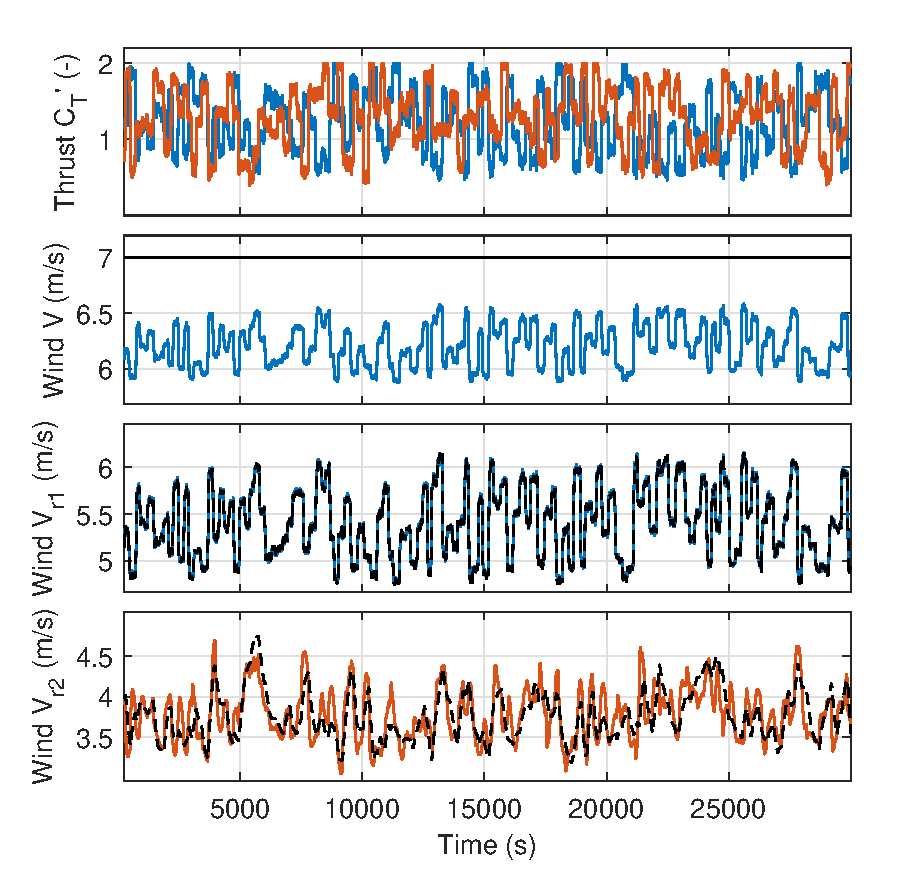
\includegraphics[width=0.485\textwidth]{figures/figures_CDC22/Fig00_AIC7mpers_OL_id.eps}}\hfill
    \subfloat[Verification dataset up to the wind speed change at $t = 5000$\,s, VAF: $V_{r1}= 100\%,\;V_{r2}=51\%$.]{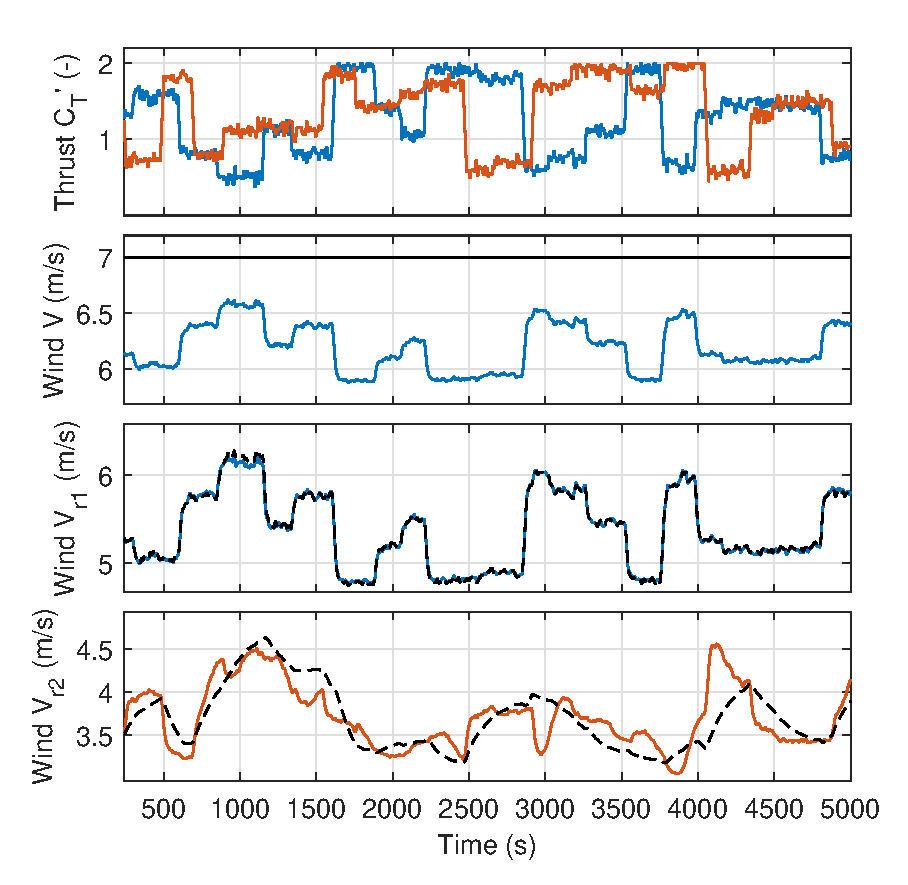
\includegraphics[width=0.485\textwidth]{figures/figures_CDC22/Fig00_AIC7mpers_OL_val.eps}}
    
    \caption[Identification and verification datasets at $V_\infty = 7$\,m/s for the Koopman model identification of the adaptive AIC algorithm]{Identification and verification datasets at $V_\infty = 7$\,m/s for the Koopman model identification of the adaptive AIC algorithm. Subplots (top to bottom): thrust $C_T^\prime$; constant wind speed $V_\infty$ (\mBlack) and $V_1$ (\mlBlue); real vs.estimated (\mlBlackDashed) effective wind $V_{r1}, V_{r2}$. WT1/WT2 signals are \mlBlue/\mlOrange.}
    \label{fig:IDdataAIC}
\end{figure}
To quantify the model's accuracy, the Variance Accounted For (VAF) value is utilized to measure the similarity between the simulated and estimated effective wind speeds. This measure of how well the output signal variation is explained by the model is also used in previous studies on Koopman DMD, e.g., \cite{Cassamo.2020}, and is defined as:
\begin{equation}
    \text{VAF} = \max \left(0, \left( 1 - \frac{\operatorname{var}(\bm{X} - \hat{\bm{X}})}{\operatorname{var}(\bm{X})} \right) \right)  \cdot 100\%
\end{equation}
where $\bm{X}$ is the simulated or real signal, $\hat{\bm{X}}$ is the estimated signal, and $\operatorname{var}(\cdot)$ denotes the variance. 

The VAF values of the two effective wind speeds differ considerably: 99.9\% for $V_{r1}$ and 49.5\% for $V_{r2}$ in the identification dataset, and 99.8\% and 51.4\% in the verification dataset. The first turbine WT1 experiences constant freestream wind and its behavior can be predicted almost exactly from the change in its thrust control signal. The second turbine is much harder to predict, as it experiences the wake of the first turbine. However, the VAF value is nearly the same for the identification and the verification dataset, i.e., the model is not overfitted to the identification data.

The third dataset, with $n_o = 29,999$ samples, and the fourth dataset, with $n_o = 9,999$ samples, are recorded at a constant freestream wind speed of 9\,m/s with the thrust levels of the first and the second dataset, respectively. The third dataset is used to identify a reference model at 9\,m/s, the fourth to verify it.


The offline-identified model, trained on the first dataset depicted in Figure~\ref{fig:IDdataAIC}(a), i.e., at a constant freestream wind speed of $7\,\mathrm{m/s}$, is validated against the entire second dataset, which includes a wind speed change. As illustrated in Figure~\ref{fig:ValComp}(a), the offline-identified model fails to track the system states once the freestream wind speed deviates from the training condition. This discrepancy occurs because the Koopman operator identified at the lower wind speed cannot capture the changes in aerodynamic sensitivity and wake dynamics at the higher wind speed. However, with the adaptive AIC algorithm, the effective wind speeds are successfully tracked again after the wind speed change. In~\cite{sharan2022Koopman}, VAF values between 86\% and 90\% were reported for the effective wind speed $V_{r2}$ using a model based solely on the two thrust inputs and evaluated under constant freestream wind conditions. However, this non-adaptive model failed to provide accurate tracking when evaluated on a dataset with varying wind speed. In~\cite{dittmer2022data}, a VAF value of 90\% was only achieved after introducing the presented update rule and including $V_1$ as an additional measurement input.

In the present study, the richer identification dataset results in a better initial Koopman matrix, such that this additional measurement is no longer required. A VAF value of approximately 80\% for $V_{r2}$ is achieved on the dataset with the wind speed change. Note that the $V_{r2}$ VAF value is higher than under constant wind speed conditions, as the wind speed change increases the variance of the signal.

\begin{figure}[ht]
    \subfloat[Non-adaptive model ($V_\infty = 7$\,m/s), VAF: $V_{r1}= 23\%,\;V_{r1}=8\%$.]{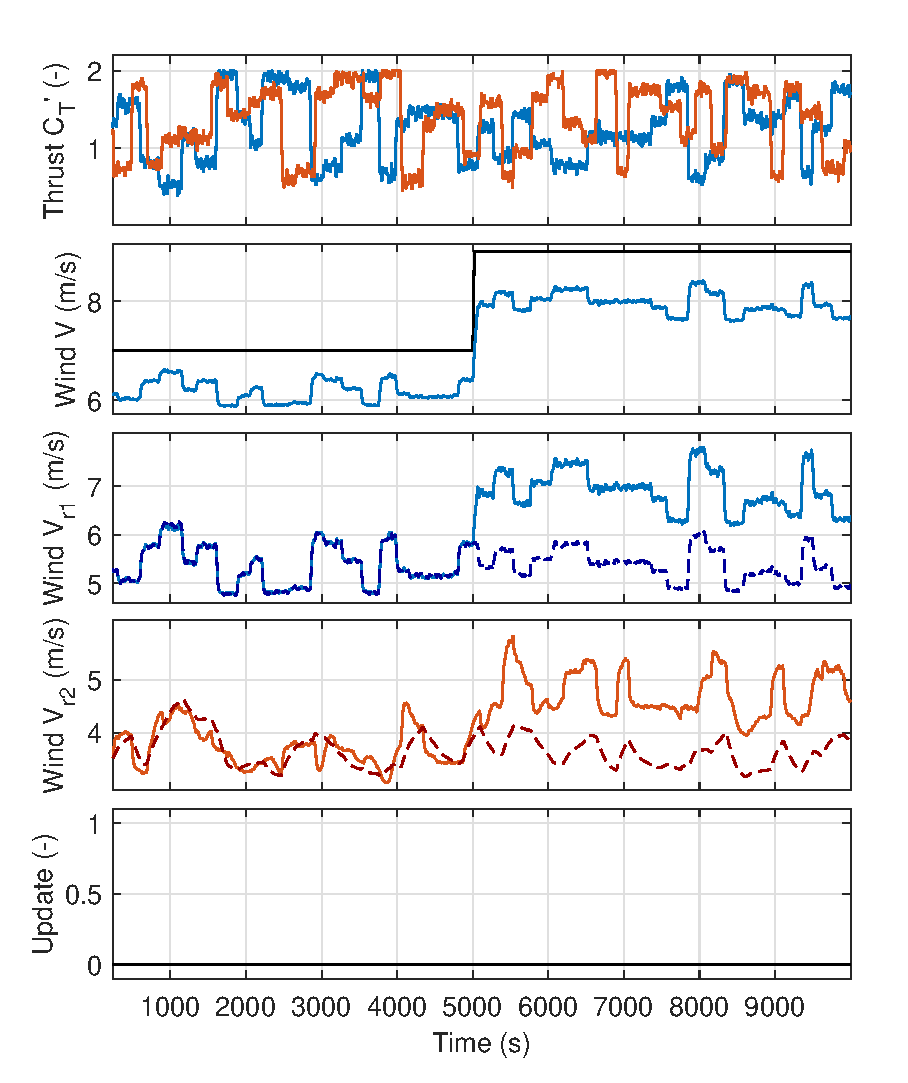
\includegraphics[width=0.485\textwidth]{figures/figures_CDC22/Fig01_OL_Update0_tex.eps}}\hfill
    \subfloat[Online-updated model,, VAF: $V_{r1}= 100\%,\;V_{r1}=80\%$]{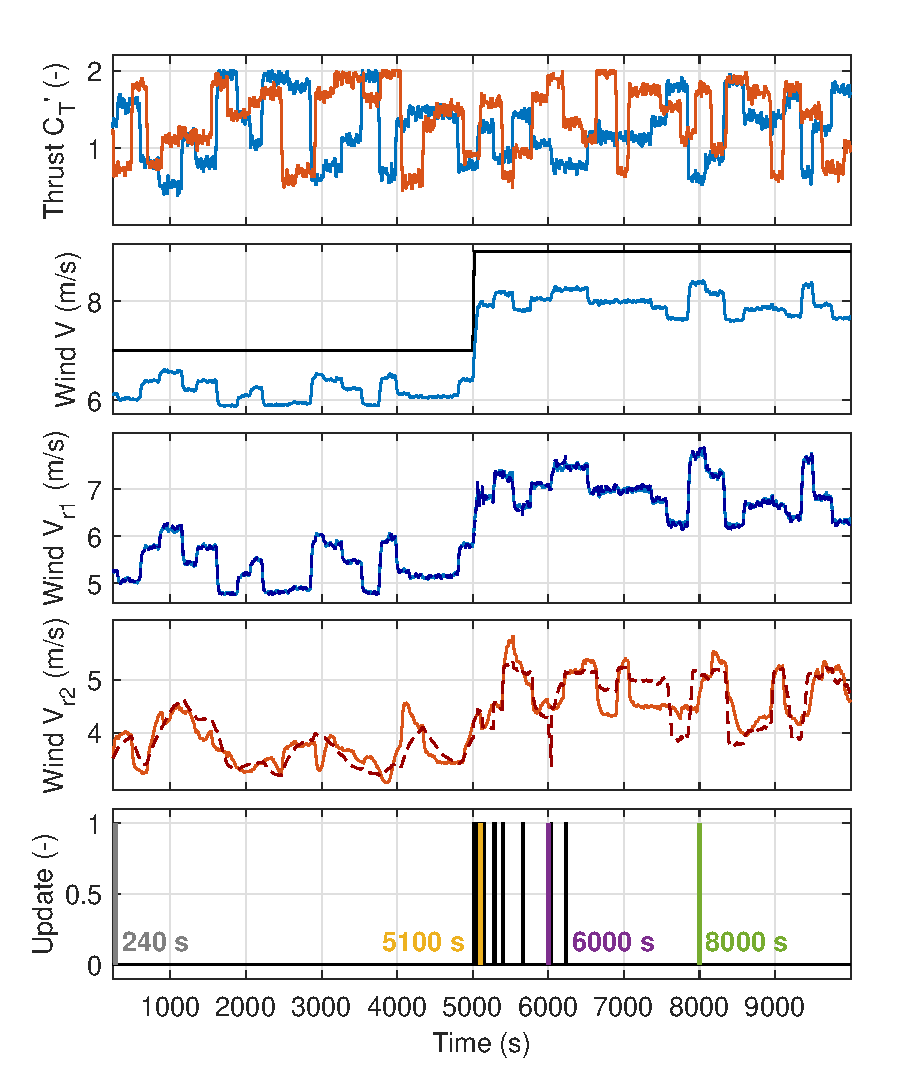
\includegraphics[width=0.485\textwidth]{figures/figures_CDC22/Fig02_OL_Update1_tex.eps}}
    \caption[Open-loop identification comparison during a wind speed step]{Open-loop identification comparison during a wind speed step at $t=5000$\,s. Subplots (top to bottom): thrust $C_T^\prime$; wind speeds $V_\infty$ (\mBlack) and $V_1$ (\mlBlue); real vs.estimated effective wind $V_{r1}$(\mlDarkBlueDashed), $V_{r2}$(\mlDarkRedDashed); and the update signal (\mBlack). WT1/WT2 signals are \mlBlue/\mlOrange.}
    \label{fig:ValComp}
\end{figure}


The first subplot in Figure~\ref{fig:ValComp}(a) shows the thrust control signals (blue for Turbine WT1, red for Turbine WT2). The second plot shows the freestream wind speed in black and the wind measured directly in front of the first turbine in blue. The third and fourth plots display the simulated effective wind speeds as solid lines and the estimated values as dashed lines. Up to the wind speed change at $t = 5000\,\mathrm{s}$, the estimates follow the real data accurately. However, after the step, the model fails to predict the effective wind speed, resulting in a significant offset and an overall VAF value of 23\% for $V_{r1}$ and 8\% for $V_{r2}$. In contrast, Figure~\ref{fig:ValComp}(b) presents the results from the online update scheme applied to the same dataset. With adaptation enabled, the estimated effective wind speeds $V_{r1}$ and $V_{r2}$ achieve VAF values of 99.8\% and 79.6\%, respectively. While the first four subplots display the same categories of signals as Figure~\ref{fig:ValComp}(a), the fifth subplot explicitly illustrates the update trigger logic. This plot indicates the instances where the model is updated because the discrepancy between the most recent five real and estimated values of $V_{r1}$ exceeded the threshold $\nu$. The 65 updates all occur between $t = 5010$\,s and $t = 6235$\,s, i.e., shortly after the wind speed change; before the change and after the adaptation, the model is not updated.

Figure~\ref{fig:SingVal} depicts the maximum and minimum singular values of four linear Koopman models at different stages of the online update process. The black dashed line represents the result of a system identification performed offline using the third dataset, recorded at a constant freestream wind speed of 9\,m/s. The colored solid lines correspond to the singular values of specific update instances at sample index $k$, which are highlighted using matching colors in the fifth subplot of Figure~\ref{fig:ValComp}(b). The initial model (grey line) is calculated on the dataset of the first open-loop simulation that does not contain the wind speed step. Note that with a sampling interval of $t_k = 1$\,s, the index $k$ corresponds directly to the simulation time in seconds. Singular values represent the gain of a system over a frequency range, with the maximum and minimum singular values defining the bounds of the system's amplification of input signals. Investigating these trajectories allows for an assessment of how the identified dynamics evolve, as shifts in the singular values indicate that the model is successfully capturing the underlying system's frequency response under varying operating conditions.
\begin{figure}[ht]
    \centering
    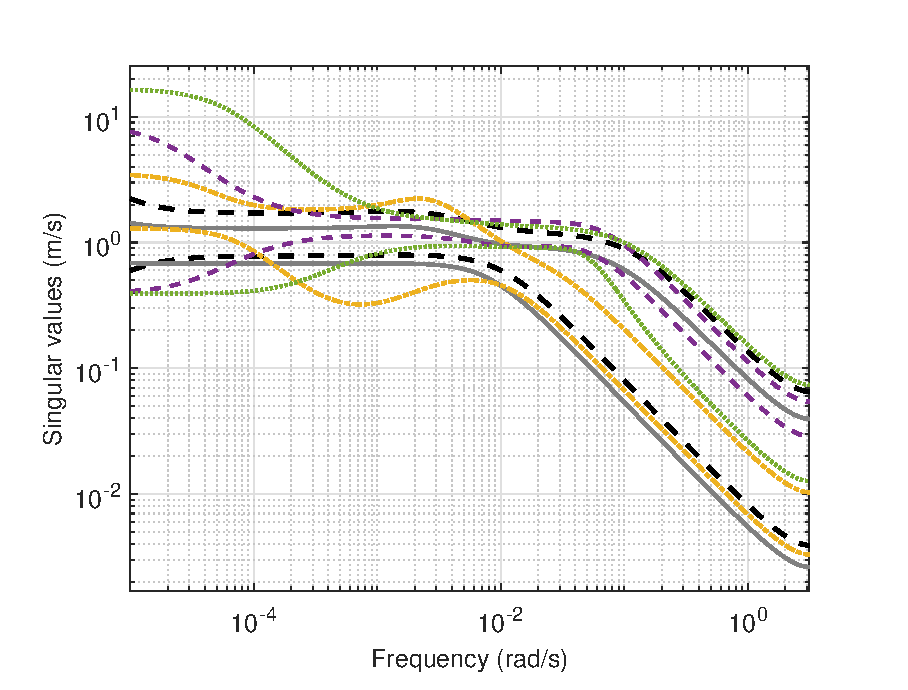
\includegraphics[width=0.65\textwidth]{figures/figures_CDC22/Fig03_OL_Bode_tex.eps}
  %  \caption[Maximum and minimum singular values of the Koopman models at various sample steps $k$ during online identification]{Maximum and minimum singular values of the Koopman models at four sample steps $k$ during online identification. Shift from the initial model ($k = 240$, \mlGray), equal to the offline identified model at a wind speed of 7\,m/s, via the models at $k= 5100$ (\mlYellowDashDot) and $k = 6000$ (\mlPurpleDashed) to the final adapted model ($k= 8000$, \mlGreenDotted), as well as the reference offline identification model (\mlBlackDashed), identified at 9\,m/s.}
    

    \caption[Maximum and minimum singular values of the Koopman models at various sample steps $k$ during online identification]{Maximum and minimum singular values of the Koopman models at four sample steps $k$ during online identification. Shift from the initial model ($k = 240$, \mlGray, the offline-identified model at 7\,m/s), through the intermediate models ($k = 5100$, \mlYellowDashDot; $k = 6000$, \mlPurpleDashed) to the final adapted model ($k = 8000$, \mlGreenDotted) is shown with the reference offline-identified model at 9\,m/s (\mlBlackDashed).}

    \label{fig:SingVal}
\end{figure}
%
\begin{itemize}
    \item The grey line ($k = 240$) represents the initial Koopman model identified at $V_{\infty} = 7\,\mathrm{m/s}$. Its frequency response differs significantly from the reference offline model (black dashed line) identified with the third dataset, obtained at $V_{\infty} = 9\,\mathrm{m/s}$: both black dashed lines show that the largest and the smallest singular values are higher by a factor of two over the depicted frequency range. However, all four lines, which are identified based on a large dataset, show nearly constant amplifications for frequencies below $0.4\,\mathrm{rad/s}$.
    \item The yellow line ($k = 5100$) shows the model after the first 25 updates following the wind speed step at $5000\,\mathrm{s}$. Its singular values have changed considerably compared with the initial model, but do not yet match those of the reference model. It can also be seen that the singular values behave reasonably as a low-pass for frequencies higher than $0.03\,\mathrm{rad/s}$. For lower frequencies, a slight 'hump' develops.
    \item The purple line ($k = 6000$) illustrates the model during the transition as more data from the $9\,\mathrm{m/s}$ regime is incorporated after 55 updates.
    \item The green line ($k = 8000$) represents the final adapted model, i.e., the model after the last of the 65 updates at $6235\,\mathrm{s}$, showing a high degree of correlation with the reference offline model for frequencies above about $10^{-3}\,\mathrm{rad/s}$. Below, the singular values of the adapted model are considerably larger than those of the reference model, as short batches of updates contain hardly any information on the static gain.
\end{itemize}
%
However, because the singular values of the adapted model match the reference model (identified at $9\,\mathrm{m/s}$) well in the relevant frequency range in which the controls influence the wind speed, the adapted model yields acceptable VAF values in open-loop, and will be shown to yield good VAF values in closed-loop tests.
The subsequent section presents closed-loop results obtained from WFSim using the adaptive Koopman model to provide effective wind speed estimates to the qLMPC controller. The value for the triggering condition $\nu$ was set to 0.15\,m/s which was found to be a good compromise between the number of updates and the accuracy of the estimation. A sensitivity study with $\nu \in \{0.02, 0.05, 0.1, 0.15, 0.3\}$\,m/s and $h \in \{5, 10, 20\}$ in the closed-loop test case described below confirms this choice: only $\nu = 0.02$\,m/s with $h = 5$ or $h = 10$ reaches a slightly lower tracking error of 13.7 and 14.0\,kW instead of 17.2\,kW, but with three times as many updates (237 and 270 instead of 80), while all other combinations shown result in tracking errors between 20 and 62\,kW. The results of the sensitivity study are listed in Table~\ref{tab:sensitivityAdaptiveAIC} at the end of this section; for $\nu = 0.10$ and $\nu = 0.05$, only the batch length $h = 5$ is shown.



\subsubsection{Closed Loop Results}
A test case is implemented to demonstrate the benefits of the adaptive Koopman MPC algorithm versus the non-adaptive scheme. The simulation is run for $5000$\,s, resulting in a dataset of $5000$ samples. At sample $k = 2000$, the freestream wind $V_\infty$ increases from $7$\,m/s to $9$\,m/s with a ramp of $0.1$\,m/s per sample. The farm power reference $P_{\text{ref}}$ is increased in a step change from $1.72$\,MW to $2.58$\,MW at sample $k = 2500$. These values were selected to ensure the wind farm is physically capable of meeting the power demand at the given wind speeds. During consecutive updates, i.e., from the second update in a row on until the error falls below the threshold again, a random signal, uniformly distributed in the range of the thrust control signals (i.e., between $0.2$ and $2$) and renewed every five samples, is added to the control signal to keep the data informative for the online identification. The control signal is not applied directly as calculated by the controller. Instead, a weighted sum is calculated, consisting of the calculated control signal multiplied by $0.99$ and the excitation signal multiplied by $0.01$. This augmented signal ensures that power tracking quality is maintained while satisfying the requirements for efficient online adaptation.

Figure~\ref{fig:CL_Comparison} compares the performance of the non-adaptive (a) and adaptive (b) Koopman MPC schemes with the update value $\nu$ set to 0.15 and the batch length $h$ set to 5. Table~\ref{tab:sensitivityAdaptiveAIC} provides a sensitivity analysis that was used as a basis to decide on these values.
%
\begin{figure}[htbp]
    \centering
    % Subfigure (a): No online update
    \subfloat[Non-adaptive AIC; TE~456.0\,kW, 1000$\cdot$AA~3.8, \;\; VAF~$V_{r1}\,/\,V_{r2}$: 0\,/\,93.7\%.] {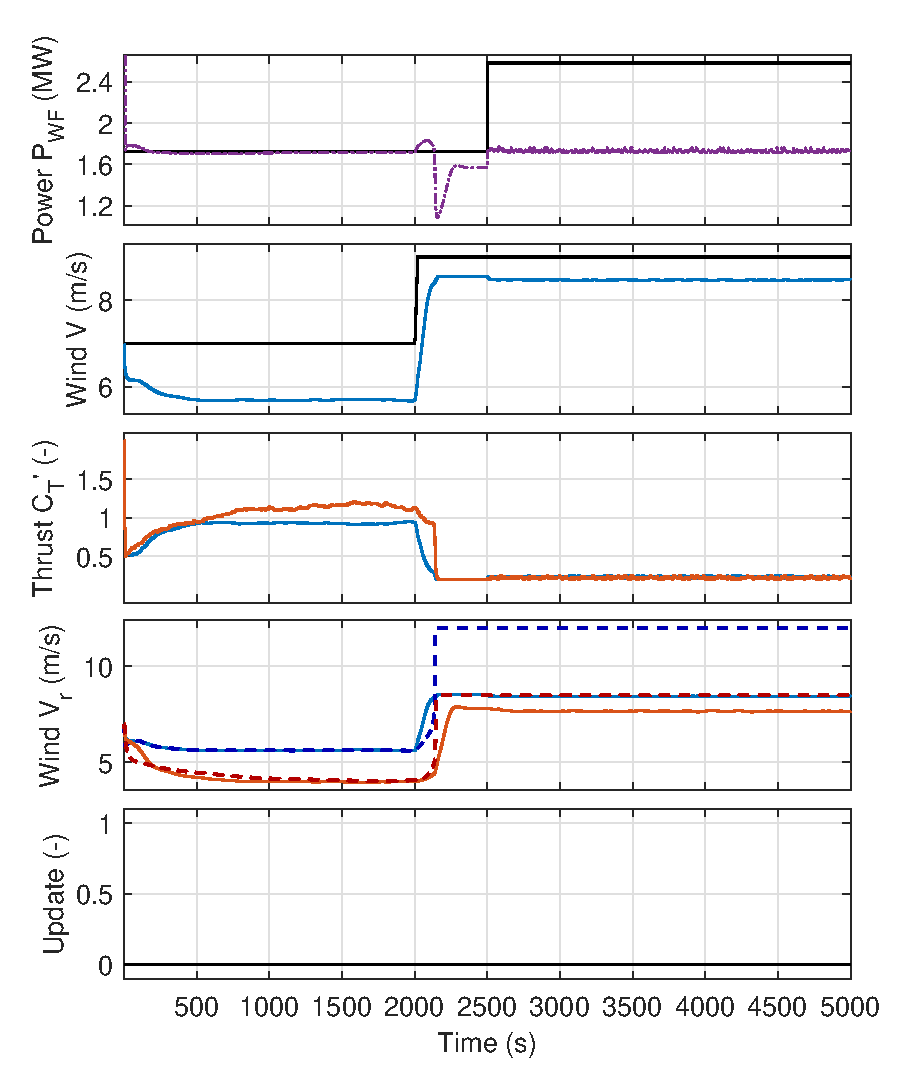
\includegraphics[width=0.495\textwidth]{figures/figures_CDC22/Fig04_CL_Update0_tex.eps}}\hfill
    \subfloat[Adaptive AIC with online updates; TE~17.2\,kW, 1000$\cdot$AA~7.6, VAF~$V_{r1}\,/\,V_{r2}$: 99.9\,/\,97.8\%.]{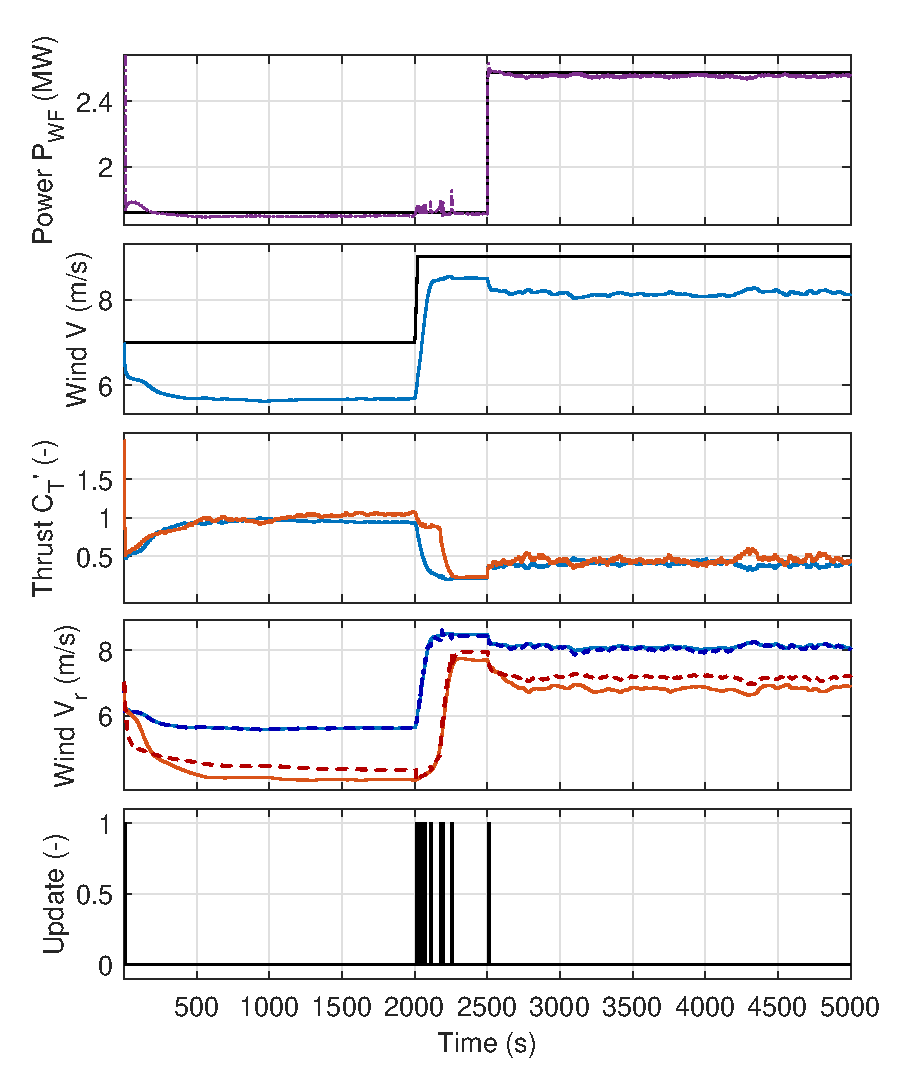
\includegraphics[width=0.495\textwidth]{figures/figures_CDC22/Fig05_CL_Update1_tex.eps}}
    \caption[Controller comparison non-adaptive and adaptive Koopman MPC AIC during a wind speed ramp and power reference step.]{Controller comparison non-adaptive and adaptive Koopman MPC AIC during a wind speed ramp and power reference step; objective mean tracking error (TE) and actuator activity (AA). Subplots (top to bottom): reference $P_{\text{ref}}$ (\mBlack) and farm power $P_{\text{WF}}$ (\mlPurpleDashed); wind speeds $V_\infty$ (\mBlack) and $V_1$ (\mlBlue); thrust $C_T^\prime$; real vs. estimated effective wind $V_{r1}$ (\mlDarkBlueDashed), $V_{r2}$ (\mlDarkRedDashed); and the update signal (\mBlack), which is zero in (a). WT1/WT2 signals are \mlBlue/\mlOrange.}
    \label{fig:CL_Comparison}
\end{figure}
%
The closed-loop performance is quantitatively evaluated using the Tracking Error (TE) and Actuator Activity (AA) criteria. While the VAF value was previously used to validate the model's open-loop predictive accuracy, it is less suited for evaluating control success. In closed-loop operation, the primary objectives are to minimize the deviation from the power reference and reduce mechanical wear. Therefore, TE and AA are used as they directly correspond to the cost function terms minimized by the controller, as defined in Equation~\eqref{eq:NMPCcostAIC}. Specifically, the TE is the mean absolute difference between $P_{\text{ref}}$ and $P_{\text{WF}}$, and the AA is the sum of the mean absolute thrust increments $|\Delta C_{Ti}^\prime|$ of the two turbines. Both TE and AA values are evaluated from $k = 240$ onward, so that the start-up of the simulation is excluded. The weighting matrices $Q = 10^{-4}$ and $R = 10^{-6}$ used in the MPC cost function, the default values of WFSim, are used as in all WFSim simulations shown in this thesis.

The top subplots in Figure~\ref{fig:CL_Comparison} illustrate the farm-level power yield $P_{\text{WF}}$ (purple) relative to the reference signal $P_{\text{ref}}$ (black). The subsequent subplots display the freestream wind speed $V_{\infty}$ alongside the local wind speed $V_1$ measured at turbine WT1, followed by the thrust control inputs $C_{T1}^\prime$ and $C_{T2}^\prime$. Consistent with the previous identification plots, signals for WT1 are shown in blue and WT2 in red. The fourth row compares the true effective wind speeds $V_{r1}$ and  $V_{r2}$ with their estimates, while the bottom row indicates the instances where the Koopman model was updated online, which occur only in Figure~\ref{fig:CL_Comparison}(b). As shown in the fourth subplot of Figure~\ref{fig:CL_Comparison}(a), the non-adaptive scheme significantly overestimates the effective wind speeds following the wind speed change: the estimate of $V_{r1}$ reaches the upper limit of 12\,m/s, and that of $V_{r2}$ is about 0.8\,m/s too high. This leads to insufficient thrust coefficients $C_{T1}^\prime$ and $C_{T2}^\prime$ of about 0.24, so that the farm power remains at about 1.73\,MW after the reference step to 2.58\,MW, resulting in a TE of 456.0\,kW. In contrast, the online-updated model in Figure~\ref{fig:CL_Comparison}(b) reduces the TE to 17.2\,kW, with VAF values of 99.9\% and 97.9\% for the estimated effective wind speeds. The model is updated 80 times: at the start of the simulation, during the wind speed change, and once after the reference step at $k = 2584$. The adaptive scheme successfully tracks the effective wind speed despite changes in both the disturbance signal ($V_{\infty}$) and the power reference ($P_{\text{ref}}$). 
%
However, the actuator activity in the adaptive case is about twice as high, $7.6\cdot 10^{-3}$ instead of $3.8\cdot 10^{-3}$. Part of this difference results from the failed tracking of the non-adaptive scheme, which keeps the thrust control signals nearly constant after the wind speed change.

Table~\ref{tab:sensitivityAdaptiveAIC} shows the sensitivity analysis used to determine the update threshold $\nu$ and the batch length $h$. The value $\nu = 0.15$ was selected because it represents a lower bound that did not trigger updates when tested with constant wind speed, unlike smaller bounds. The open-loop VAF value of the effective wind speed of the first turbine is not shown, as it is at least 99.5\% for all adaptive cases, compared with 23.2\% for the non-adaptive case, see Figure\ref{fig:ValComp}(a). When $\nu$ was doubled to $0.30$, the closed-loop tracking error increased by roughly 17\% (from $17.2\,\mathrm{kW}$ to $20.2\,\mathrm{kW}$) because the update algorithm triggered too late. It was also tested whether $\nu$ could be further decreased; however, values of $0.10$ and $0.05$ increased rather than decreased the tracking error compared with the selected setting. The trigger value had to be lowered to $0.02$ to decrease the tracking error below that of the selected value of $0.15$. It is assumed that the advantage of acquiring fresh information on a model that already fits well during constant wind speed is offset by the disadvantages of triggering updates unnecessarily and by the more frequent injection of the excitation signal into the controls during consecutive updates. This problem can apparently be mitigated by setting the value of $\nu$ to $0.02$, which enforces the predictions to be close to the current trajectory. But setting $\nu$ to $0.02$ increases the closed-loop number of updates nearly threefold, from $80$ to $237$. Therefore, the trigger threshold was set to $0.15$ as a compromise between tracking error and update frequency.

It was also investigated whether using more samples per update would be advantageous. Increasing the batch length $h$ was disadvantageous for the three threshold values 0.02, 0.15 and 0.3: the closed-loop tracking error increased with $h$, and $h = 20$ combined with $\nu = 0.15$ led to an open-loop VAF value of $V_{r2}$ of 0\%. This is attributed to the update mechanism: as the trigger evaluates the errors of the last $h$ samples, estimated with the model before the update, a single large error triggers up to $h$ consecutive updates with overlapping batches, and the normalization by the number of consecutive updates reduces the weight of the previous data. The model is then dominated by few, repeatedly weighted samples with nearly constant effective wind speeds, for which the lifted states $V_{ri}$, $V_{ri}^2$, and $V_{ri}^3$ are nearly linearly dependent. The correlation matrix $\mathbf{L}_u$ inverted in the update becomes ill-conditioned, so that small errors in the data cause large changes of the Koopman matrix and can deteriorate the predictions considerably.

It should be also noted that, while all combinations of threshold and batch length resulted in smaller tracking errors than the non-adaptive algorithm, they increased the actuator activity. A similar sensitivity analysis regarding the weighting factors of the excitation signal and the calculated control signal, which are currently set to 0.01 and 0.99, is future work.

\begin{table}[htbp]
    \centering
    \caption[Sensitivity of the adaptive AIC to the update settings]{Sensitivity of the adaptive AIC to the trigger threshold $\nu$ and the batch length $h$ of the online update; selected setting in bold. The number of model updates is $N_\text{upd}$. Open loop: VAF values of the validation data with the wind ramp from 7 to 9\,m/s at $k = 5000$ (evaluated from $k = 240$; VAF values below 0 are set to 0). Closed loop: qLMPC with the wind ramp from 7 to 9\,m/s at $k = 2000$; TE: tracking error, AA: actuator activity.}
    \label{tab:sensitivityAdaptiveAIC}
    \begin{tabular}{rr cc cccc}
        \toprule
        & & \multicolumn{2}{c}{Open loop} & \multicolumn{4}{c}{Closed loop} \\
        \cmidrule(lr){3-4} \cmidrule(lr){5-8}
        $\nu$ (m/s) & $h$ & $N_\text{upd}$ & VAF $V_{r2}$ (\%) & $N_\text{upd}$ & TE (kW) & AA ($10^{-3}$) & VAF $V_{r2}$ (\%) \\
        \midrule
        \multicolumn{2}{l}{non-adaptive} & 0 & 8.0 & 0 & 456.0 & 3.82 & 93.7 \\
        \midrule
        0.30 & 5 & 60 & 76.4 & 55 & 20.2 & 7.11 & 93.7 \\
        0.30 & 10 & 130 & 75.4 & 90 & 32.6 & 7.79 & 91.6 \\
        0.30 & 20 & 200 & 73.2 & 113 & 46.7 & 8.10 & 91.3 \\
        \midrule
        $\bm{0.15}$ & $\bm{5}$ & \textbf{65} & \textbf{79.6} & \textbf{80} & \textbf{17.2} & \textbf{7.58} & \textbf{97.9} \\
        0.15 & 10 & 160 & 74.4 & 100 & 25.5 & 7.87 & 96.4 \\
        0.15 & 20 & 200 & 0.0 & 120 & 61.7 & 8.08 & 93.0 \\
        \midrule
        0.10 & 5 & 95 & 60.9 & 85 & 41.8 & 6.89 & 84.8 \\
       % 0.10 & 10 & 150 & 77.8 & 110 & 22.1 & 7.41 & 94.5 \\
        %0.10 & 20 & 360 & 0.0 & 160 & 31.1 & 8.06 & 88.3 \\
        %\midrule
        0.05 & 5 & 290 & 82.9 & 131 & 42.5 & 8.63 & 86.8 \\
        %0.05 & 10 & 460 & 79.4 & 168 & 55.7 & 8.60 & 89.7 \\
        %0.05 & 20 & 360 & 71.3 & 180 & 99.6 & 5.83 & 4.1 \\
        \midrule
        0.02 & 5 & 615 & 88.2 & 237 & 13.7 & 7.37 & 96.7 \\
        0.02 & 10 & 1000 & 86.2 & 270 & 14.0 & 7.40 & 98.8 \\
        0.02 & 20 & 1580 & 88.1 & 364 & 26.8 & 6.81 & 85.6 \\
        \bottomrule
    \end{tabular}
\end{table}

All closed-loop results are obtained with the effective wind speeds estimated from the measured turbine powers with Equation~\eqref{eq:VrFromPower}. With the effective wind speeds of the WFSim flow field instead, which were used in \cite{dittmer2022data}, the adaptive scheme reaches a TE of 13.3\,kW with an AA of $7.55\cdot 10^{-3}$, while the TE of the non-adaptive scheme is unchanged at 456.0\,kW. As the estimates deviate by at most 0.003\,m/s, this difference of 4\,kW is mainly caused by slightly shifted update times, which change the subsequent closed-loop trajectory, rather than by the estimation error itself.

It should be noted that the precise and fast power tracking achieved by the adaptive Koopman MPC is partly attributable to the simplified turbine modeling in WFSim. The turbines are represented as actuator disks with a first-order filter on the thrust control signal, see Equation~\eqref{eqPowerWTAIC_vector}, while rotor inertia, drive-train and structural dynamics, and the turbine controllers are not modeled. In a higher-fidelity setup, the tracking response would likely be limited by mechanical time constants and structural load constraints. Therefore, while these results show the advantage of the adaptive over the non-adaptive Koopman approach, further validation with aeroelastic tools is necessary to assess the performance under realistic mechanical constraints.

The adaptive Koopman approach shows that effective wind speeds in waked wind farms can be predicted online with a data-driven model, even if the operating conditions are not covered by the training data. Since the model is only updated when the prediction error exceeds the threshold $\nu$, the computational effort remains low, while the prediction accuracy is maintained, with VAF values of nearly 100\% for the upstream turbine and of 80\% in open loop and 98\% in closed loop for the downstream turbine. In the closed-loop case, the adaptive strategy reduces the power tracking error by about 96\% compared to the non-adaptive scheme, at the cost of an actuator activity that is about twice as high. These results indicate that adaptive Koopman models are a suitable basis for wind farm control under varying freestream conditions. The following section builds upon this framework by integrating yaw control, exploring how WRC can be used alongside thrust control to further optimize total farm yield.
% Created by runSensitivityAdaptiveAIC on 2026-10-29
% Adaptive AIC without V1: trigger threshold nu and window/batch length h of the online update


\section{Wind Farm MPC with Combined Yaw and Thrust Control} 
\label{sec:WindFarmLinearMPCforWRC-AIC}

The control design presented in Section~\ref{sec:AdaptiveWindFarmqLMPCforAIC} is extended to include yaw control in addition to thrust control. Two data-driven WRC-AIC wind farm control approaches based on Koopman model predictive control are proposed and compared to a baseline AIC scheme. These WRC-AIC algorithms combine thrust and yaw control for power reference tracking and yield optimization:
\begin{enumerate}
    \item \textbf{Prescribed yaw (Gaussian wake model):}  
    The upstream turbine's yaw angle is computed to maximize power yield, while the thrust control signals of both turbines are determined via MPC to minimize power tracking error and thrust variations. In \cite{dittmer2023koopman}, both control actions are based on estimated effective wind speeds obtained from a Koopman model with the control signals as inputs and the two effective wind speeds as outputs, as described in Section~\ref{sec:AdaptiveWindFarmqLMPCforAIC}, and the thrust signals are determined via qLMPC. In this thesis, the farm power is predicted with the Koopman model of the second approach.
    
    \item \textbf{Joint yaw and thrust optimization:}  
    The upstream turbine's yaw angle and thrust coefficients are optimized simultaneously via linear MPC to minimize power tracking error as well as variations in thrust and yaw. In this case, the controller operates directly on the estimated total farm power, which is derived from a separate Koopman model identified with the same inputs as the first model but with the total wind farm power as the output. In this thesis, this Koopman model is also used for the first approach and for the baseline AIC, see Section~\ref{qLMPCDesign}.
\end{enumerate}
The first approach follows the concept introduced in \cite{boersma2017tutorial}. It verifies whether the power reference exceeds the so-called greedy power of the wind farm, defined as the power obtained when both turbines operate without yaw misalignment and at maximum thrust. If this condition is met, the yaw angle is gradually increased to an offline-calculated value that maximizes the overall wind farm yield. The second approach investigates whether smoother control signals can be achieved by jointly optimizing all available control inputs.

The test case corresponds to the same wind farm setup consisting of two turbines introduced in Section~\ref{sec:WindFarmSimulationWFSim} and used in Section~\ref{sec:AdaptiveWindFarmqLMPCforAIC}, with the wind direction aligned with the main axis of the farm. The two Koopman MPC designs leveraging combined WRC-AIC significantly reduce the tracking error compared to the previously presented baseline AIC algorithm. It is also demonstrated that this improvement can be achieved with relatively small yaw angles, thereby avoiding excessive mechanical loads on turbines operating with yaw misalignment. This makes the proposed approach a promising candidate for further investigation in three-dimensional medium- and high-fidelity simulation environments.

\subsection{Simulation Setup for Combined Yaw and Thrust Control} \label{WakeModel} 
As before, WFSim is used to obtain open-loop data and for closed-loop controller testing. This section provides an overview of the WFSim environment and describes the specific test cases utilized for Koopman system identification in this context.

Figure~\ref{fig:BlockDiagramFarm} illustrates the underlying concept for the WRC-AIC strategies applied to the two-turbine wind farm. Note that the primary difference from the setup in Section~\ref{sec:AdaptiveWindFarmqLMPCforAIC} is that the yaw control signal of the upstream turbine WT1, $\gamma_1$, is now an active control variable.
%
\begin{figure}[h]
    \centering
    \includegraphics[width=0.9\textwidth]{figures/figuresBlockDiagram_IFAC23/farmCtrl17_P_multVthesis_WRCAIC_EIODMD.pdf}
    \caption[Block diagram of WFSim for WRC-AIC]{Block diagram of WFSim for WRC-AIC with farm control inputs $P_{\text{ref}}$, $P_1$, $P_2$, control signals $C_{T1}^{\prime}$, $C_{T2}^{\prime}$, $\gamma_1$, freestream wind $V_\infty$, and wind $V_1 = V_{1_m}$. Wind speeds directly in front and behind the $i$-th turbine are $V_{i_1}$ to $V_{i_{n_r}}$ and $V_{i\text{out}_1}$ to $V_{i\text{out}_{n_r}}$. The input to the EDMD model (\mlOldBlue) are $C_{T1}^{\prime}$ and  $C_{T2}^{\prime}$, its outputs are the effective wind outputs $V_{r1}$ and $V_{r2}$. The input to the EIODMD model (\mlRed) are $C_{T1}^{\prime}, C_{T2}^{\prime}$, and $\gamma_1$, its output is the farm power $P_{\text{WF}} = P_1 + P_2$.}
    \label{fig:BlockDiagramFarm}
\end{figure}
%
The signals are defined as in previous sections. Notable differences are that the freestream wind speed is kept constant and $\gamma_1$ is commanded by the farm controller. This results in the following simulation setup and signals:
\begin{itemize}
    \item[-] The freestream wind $V_\infty$ is constant at $8$\,m/s and aligned with the main axis of the farm for all simulations in this section.
    \item[-] The farm power reference $P_{\text{ref}}$.
    \item[-] The measured wind $V_1$ at WT1, which was a controller input in \cite{dittmer2022data} and \cite{dittmer2023koopman}; in this thesis, it is only recorded and displayed.
    \item[-] The thrust control signal $C_{T1}^{\prime}$ and yaw $\gamma_1$ of WT1, with the latter being a variable here, while it was fixed at 0\textdegree~in Section~\ref{sec:AdaptiveWindFarmqLMPCforAIC}.
    \item[-] The effective wind speed $V_{r1}$ (mean wind speed over the rotor disk) and power $P_1$ of WT1, with $V_{r1}$ estimated from $P_1$ with Equation~\eqref{eq:VrFromPower} in closed loop.
    \item[-] Corresponding input and output signals for turbine WT2.
\end{itemize}
The farm layout and turbine parameters follow Table~\ref{table:WfSim}. As for the AIC, the controllers use the effective wind speeds $\tilde{V}_{ri}$ estimated from the powers $P_i$ with Equation~\eqref{eq:VrFromPower}, i.e., with the known, yaw-dependent power coefficient.

Previous publications utilizing WFSim~\cite{boersma2017tutorial,doekemeijer2018online, sharan2022Koopman, dittmer2022data} focused on thrust control $C_T^{\prime}$ for AIC, resulting in $n_u = n_{\text{WT}}$ control inputs. However, WFSim also supports yaw control $\gamma$ for wake redirection. In a two-turbine scenario, this could result in $2n_{\text{WT}}$ inputs; however, for this proof of concept, only the yaw of the first turbine is varied. Since the second turbine has no downstream neighbors, its optimal orientation remains $\gamma_2 = 0$\textdegree{}, resulting in $n_u = 3$ control inputs for this study.

Open-loop WFSim simulations are used to generate data for system identification, where, as before, one sample $k$ corresponds to $1$\,s. As in Section~\ref{sec:AdaptiveWindFarmqLMPCforAIC}, new signals were created for that purpose:
\begin{itemize}
    \item In \cite{dittmer2023koopman}, a signal with $n_o = 31,499$ samples was created. Up to sample 28,000, the thrust signals $C_{T1}^{\prime}$ and $C_{T2}^{\prime}$ are constructed from white noise (mean 1.7, variance 0.3, lower and upper limits 0.1 and 2.0, respectively) held constant for $5$\,samples, and the yaw signal $\gamma_1$ is stepped by $5$\textdegree{} every $4000$\,samples from $0$\textdegree{} to $30$\textdegree{} and augmented with zero-mean band-limited noise (variance $0.5$\textdegree{}); afterwards, the thrust signals are set to 2 and the yaw angle is reduced in steps of 5\textdegree{} every 500 samples back to 0\textdegree{}. 
    \item The signal designed for this thesis has $n_o = 29,999$ samples: the thrust signals of both turbines and the yaw angle of WT1 jump independently between random levels, as for the AIC in Section~\ref{sec:AdaptiveWindFarmqLMPCforAIC}, with thrust levels between 0.5 and 2, yaw levels between 0\textdegree{} and 30\textdegree{}, hold times of 150 to 300\,s, small additive noise (standard deviations 0.05 and 0.5\textdegree{}), and rate limits of 0.05\,s$^{-1}$ and 1\textdegree/s.
\end{itemize}
Both datasets are used from sample 240 on, after the wake is established, and are appended for the identification. These signals ensure data excitation across all relevant frequencies and control input combinations.

%
\subsection{Lifting Functions for Combined Yaw and Thrust Control}\label{sec:lifting functions for Combined Yaw and Thrust Control}
The power of an actuator disk depends nonlinearly on the thrust control signal and the yaw angle. To keep the Koopman model linear in the control signals $\bm{u} = [C_{T1}' \;\; C_{T2}' \;\; \gamma_1]^T$, the nonlinear functions are not applied to the control signals themselves but to the filtered control signals $\hat{\bm{u}} = [\hat{C}_{T1}' \;\; \hat{C}_{T2}' \;\; \hat{\gamma}_1]^T$, which are additional states of the model:

\begin{equation} \label{eq:FiltInputs}
    \hat{\bm{u}}(k+1) = (1-\tau)\,\hat{\bm{u}}(k) + \tau\,\bm{u}(k),
\end{equation}
with the filter coefficient $\tau$ of the turbine model in Equation~\eqref{eqPowerWTAIC_vector}, i.e., $\tau = 0.18$ for the time constant of 5\,s at the sampling time of 1\,s. The MPC applies its decision variables with this filter, see Section~\ref{qLMPCDesign}, so that $\hat{\bm{u}}(k)$ are the control signals applied to the turbines in the previous sample. Accordingly, in the open-loop identification data, $\hat{\bm{u}}(k)$ is the applied control signal of the previous sample, and $\bm{u}(k)$ is obtained by inverting the filter. From the filtered control signals, the features

\begin{equation} \label{eq:InputFeatures}
    g_1 = \frac{\hat{C}_{T1}'\cos^3\hat{\gamma}_1}{(1 + \hat{C}_{T1}'/4)^3}, \quad g_2 = \frac{\hat{C}_{T2}'}{(1 + \hat{C}_{T2}'/4)^3}, \quad a_1 = \frac{\hat{C}_{T1}'/4}{1 + \hat{C}_{T1}'/4}, \quad a_c = a_1\cos^2\hat{\gamma}_1
\end{equation}
are calculated.
%
These are used to include wake dynamics into the Koopman model. The rationale behind these features is that the features $g_1$ and $g_2$ are proportional to the power coefficients of the two actuator disks:
\begin{itemize}
    \item The axial induction of turbine $i$ is $a_i = (C_{Ti}'/4)/(1+C_{Ti}'/4)$.
    \item The power of turbine $i$ in a uniform freestream inflow $V$ is $\frac{1}{2}\rho_a A_r C_{Ti}' (1-a_i)^3 V^3 = \frac{1}{2}\rho_a A_r\, C_{Ti}'/(1+C_{Ti}'/4)^3\, V^3$.
    \item This is reduced by $\cos^3\gamma_1$ for the yawed turbine.
\end{itemize}
From $\hat{C}_{T1}'$, $\hat{\gamma}_1$, and the features $a_1$ and $a_c$ in Equation~\eqref{eq:InputFeatures}, moving means are calculated. They are included directly in the feature vector as well as in products with the feature $g_2$ at sample $k$:
\begin{itemize}
    \item The signals $M_{C}$, $M_{\gamma}$, $M_{a}$, and $M_{ac}$ are exponential moving means of $\hat{C}_{T1}'$, $\hat{\gamma}_1$ (in degrees), $a_1$, and $a_c$ with a time constant of 100\,s, i.e., the filter coefficient $\tau_M = 0.01$:
    \begin{equation} \label{eq:MovingMeans}
        \bm{M}_{\text{mean}}(k+1) = (1 - \tau_M)\, \bm{M}_{\text{mean}}(k) + \tau_M\,\bm{h}(k), \quad \bm{h} = [\hat{C}_{T1}' \;\; \hat{\gamma}_1 \;\; a_1 \;\; a_c]^T.
    \end{equation}
    They represent the delayed effect of the induction and the wake deflection of the upstream turbine on the downstream turbine.
    \item The products of $g_2$ with $M_{a}$, $M_{\gamma}$, and $M_{ac}$ represent the interaction of these effects with the thrust of the downstream turbine.
\end{itemize}
%
The feature vector
\begin{equation} \label{eq:wFeatWRC}
    \bm{w}(k) = [\underbrace{\hat{C}_{T1}' \;\; \hat{C}_{T2}' \;\; \hat{\gamma}_1}_{\hat{\bm{u}}^T} \;\; \underbrace{g_1 \;\; g_2\;\; a_1\;\; a_c}_{\bm{g}^T} \;\; \underbrace{M_{C} \;\; M_{\gamma} \;\; M_{a} \;\; M_{ac}}_{\bm{M}_{\text{mean}}^T} \;\; \underbrace{g_2 M_{a} \;\; g_2 M_{\gamma} \;\; g_2 M_{ac}}_{\bm{M}_{g,\text{mean}}^T}]^T \in \mathbb{R}^{14},
\end{equation}
together with the lifted state used for EDMD,
\begin{equation}
    \bm{\varphi}_{\text{EDMD}} = [\bm{x}^T \;\; (\bm{x}^2)^T \;\; (\bm{x}^3)^T]^T \in \mathbb{R}^{6}, \quad \text{with} \quad \bm{x} = [V_{r1} \;\; V_{r2}]^T,
\end{equation}
forms a new, extended lifted state. The lifted state and the output for EIODMD are
%
\begin{equation}
    \bm{\varphi}_{\text{EIODMD}}= [\bm{w}^T \quad  \bm{\varphi}_{\text{EDMD}}^T \quad d_{\text{bias}}]^T \in \mathbb{R}^{21}, \quad \text{and} \quad \bm{y}(k) = P_{\text{WF}}(k).
\end{equation}
%
The bias state $d_{\text{bias}} = 1$ adds a constant offset to the state and output equations, corresponding to the intercept in linear regression. For simplicity, the new lifted state is named $\bm{\varphi} = \bm{\varphi}_{\text{EIODMD}}$ in this chapter.

The model is built in two steps. First, a control-affine model is identified with EIODMD, with the lifted effective wind speeds $\bm{\varphi}_{\text{EDMD}}$ as states, the farm power as output, and the feature vector $\bm{w}$, the bias, and the control signals $\bm{u}$ as inputs. Its rows for the lifted effective wind speeds and for the output are linear in $\bm{w}$ and $\bm{u}$ and are therefore taken over unchanged into the linear model, in which the features become states. Second, the rows of the additional states are set up: the rows of the filtered control signals, Equation~\eqref{eq:FiltInputs}, of the moving means, Equation~\eqref{eq:MovingMeans}, and of the bias state are known and set to their filter dynamics. Only the propagation of the nonlinear features $g_1$, $g_2$, $a_1$, $a_c$ and of the products $\bm{M}_{g,\text{mean}}$ is approximated linearly; these rows are identified by least squares from the identification data, with the feature states and the control signals as regressors. The resulting linear model
\begin{align}\label{eq:Koop2}
    \hat{K}_{2} = \left[\begin{array}{c|c} \bm{A}_{\hat{K}2}  & \bm{B}_{\hat{K}2}\\ \hline \bm{C}_{\hat{K}2}  & \bm{D}_{\hat{K}2} \end{array}\right] \in \mathbb{R}^{22\times24},
\end{align}
with
\begin{align*}
    \bm{A}_{\hat{K}2} \in \mathbb{R}^{21\times21},\; \bm{B}_{\hat{K}2}\in \mathbb{R}^{21\times3},\; \bm{C}_{\hat{K}2} \in \mathbb{R}^{1\times21},\;\; \bm{D}_{\hat{K}2}\in \mathbb{R}^{1\times3},
\end{align*}
provides predictions of the effective wind speeds $V_{r1}$ and $V_{r2}$ as well as of the farm power $P_{\text{WF}}$. The row of the bias state in $\bm{A}_{\hat{K}2}$ consists of zeros except for the value 1 in its 21st element, and the corresponding row of $\bm{B}_{\hat{K}2}$ is zero. Hence, the bias state stays at one and contributes the eigenvalue 1, which only represents the constant offset. The largest magnitude of the remaining eigenvalues of $\bm{A}_{\hat{K}2}$ is 0.9985, i.e., the identified model is stable.
The matrices of Equation~\eqref{eq:Koop2} are used in the QP solved at each sample of the MPC as follows.



%

\subsection{MPC Design for Combined Yaw and Thrust Control} \label{qLMPCDesign} 
Similar to the previously discussed AIC algorithm, the objective of the WRC-AIC wind farm controllers is to achieve accurate power reference tracking while minimizing changes in the control inputs. The WRC-AIC extends the previous approach by including the yaw of the first turbine as an additional control input, alongside the already used thrust control signals, which requires adjustments to the objective function and control algorithm. The main benefit of incorporating yaw, which is an increase in the achievable wind farm power output, will be demonstrated in the results presented in Section~\ref{SimResults}. In this section, the cost function to be optimized is defined, and the two MPC designs, both based on the Koopman matrix $\hat{K}_2$, are discussed.

The cost function $J(\bm{U})$ for both WRC-AIC schemes is formulated identically to the AIC algorithm, as given in Equation~\eqref{eq:errortraject}. It is based on the trajectories of the tracking error $\bm{E}$ and the changes in the control input $\Delta \bm{U}$:
\begin{align*} 
    J(\bm{U}) = \underbrace{\bm{E}^T \bm{Q} \bm{E}}_{J_Q (\bm{U})} + \underbrace{\Delta \bm{U}^T \bm{R} \Delta \bm{U}}_{J_R (\bm{U})},
\end{align*}
over a prediction horizon of $n_h$ sample steps. The weighting matrices are based on the scalar weights $Q$ and $R$, with the weight on the power error derived as $\bm{Q} = Q \bm{I}_{n_h}$, as before. The weight on the control input changes is defined as
\begin{align*}
    \bm{R} = R \, \bm{I}_{n_h} \otimes \mathrm{diag}(R_{u1}, R_{u2}, R_{u3}),
\end{align*}
allowing differentiation of the penalty on changes in the different control inputs.

Correspondingly, the future error trajectory is $\bm{E}_k = \bm{P}_{\text{ref},k} - \bm{P}_{\text{WF},k}$, which is based on the total wind farm power. The change in control inputs is calculated as in Equation~\eqref{eq:DUAIC}.
%
For the two-turbine wind farm controlled with three control inputs and the default WFSim setting $n_h = 10$, the control trajectory is defined as the vector
\begin{align*} 
    \bm{U}_{K2}(k) &= \begin{bmatrix} 
        C_{T1}^\prime(k) & C_{T2}^\prime(k) & \gamma_1(k) & \dots & \gamma_1(k+n_h-1) 
    \end{bmatrix}^T \in \mathbb{R}^{n_{hu} \times 1}.
\end{align*}
with $n_{hu} = n_h\cdot n_u = 30$. The cost function summands can be written with $\bm{U} = \bm{U}_{K2}$ as:
\begin{align*} 
    J_Q (\bm{U}) &= \big(\bm{P}_{\text{ref}} - (\tilde{\bm{L}} \bm{x}_0 + \tilde{\bm{S}} \bm{U})\big)^T \bm{Q} \big(\bm{P}_{\text{ref}} - (\tilde{\bm{L}} \bm{x}_0 + \tilde{\bm{S}} \bm{U})\big),\\
    J_R (\bm{U}) &= \Delta \bm{U}^T \bm{R} \Delta \bm{U},
\end{align*}
where the initial state $\bm{x}_0 = \bm{\varphi}(k) \in \mathbb{R}^{21}$ is the lifted state at the current sample, and the matrices $\tilde{\bm{L}} \in \mathbb{R}^{n_h \times 21}$ and $\tilde{\bm{S}} \in \mathbb{R}^{n_h \times n_{hu}}$ are used to calculate the expected future trajectory of the wind farm power $\bm{P}_{\text{WF}}$.

In the first WRC-AIC approach, the optimal yaw angle $\gamma_1^*$ is computed using the Gaussian wake model from~\cite{bastankhah2016experimental}, ensuring comparability with~\cite{boersma2019constrained}. Whenever the power reference exceeds the greedy power, the yaw angle is moved toward $\gamma_1^*$; otherwise, it is moved toward 0\textdegree. During the transition from 0\textdegree~to $\gamma_1^*$, the reference yaw is smoothed with the first-order filter of the turbine model and a rate limit of 1\textdegree/s. The resulting yaw trajectory is prescribed over the prediction horizon, and only the thrust signals are optimized. In \cite{dittmer2023koopman}, the thrust signals for the baseline AIC and the AIC with static optimal yaw were calculated via the qLMPC AIC algorithm described in Section~\ref{sec:AdaptiveWindFarmqLMPCforAIC}, using the intermediate step of predicting the effective wind speeds and calculating the wind farm power from them. In this thesis, the farm power is instead predicted using $\hat{K}_2$ for all three MPC schemes, such that the baseline AIC and the two WRC-AIC approaches differ only in their treatment of the yaw angle. The baseline AIC uses the same MPC formulation, with the yaw angle fixed at $0^\circ$. The designs differ only in the bounds imposed on the yaw angle:
\begin{itemize}
    \item For the baseline AIC and the first WRC-AIC approach, the lower and upper bounds of $\gamma_1$ are set to an equal target at every prediction step, thereby prescribing a constant yaw trajectory as described above. As the decision variables are the control signals before the filter of Equation~\eqref{eq:FiltInputs}, the bounds are set to the yaw values that result in the prescribed trajectory after the filter; the rate limit of the yaw decision variable is not applied in this case. The target is $0^\circ$ for the baseline AIC and either $0^\circ$ or $\gamma_1^*$ for the first WRC-AIC approach. This was differently addressed in \cite{dittmer2023koopman}, where the constant yaw angle was handled as a state, resulting in $n_{hu} = 20$ for two turbines and a prediction horizon of $n_h = 10$. 
    \item In the second WRC-AIC approach, $\gamma_1$ is bounded between $0^\circ$ and $22^\circ$ and optimized jointly with the thrust signals.
\end{itemize}
Thus, the yaw angle is not treated as a disturbance state but remains an input to the prediction model. For the baseline AIC and the WRC-AIC approach using the constant yaw angle  $\gamma_1^*$, the fixed bounds leave the QP no freedom to optimize $\gamma_1$, making it equivalent to the formulation with $n_u = 2$ described above. Nevertheless, the predicted effect of the prescribed, constant yaw trajectory on farm power, including its effect on the moving means, is accounted for when optimizing the thrust signals.

In the joint optimization of the thrust and yaw controls, the wind farm power $\bm{P}_{\text{WF}}$ is predicted directly with the Koopman model, without the effective wind speeds as scheduling parameters of the WFSim farm model. This is a linear model, and the stacked Toeplitz matrices $\bm{\Lambda}_{\hat{K}2}$ and $\bm{S}_{\hat{K}2}$ are constructed from the matrices $\bm{A}_{\hat{K}2}, \bm{B}_{\hat{K}2}, \bm{C}_{\hat{K}2}, \bm{D}_{\hat{K}2}$, presented in Equation~\eqref{eq:Koop2}, as:
\begin{align*}
    \bm{\Lambda}_{\hat{K}2} &= \begin{bmatrix}
        \bm{C}_{\hat{K}2} \\
        \bm{C}_{\hat{K}2} \bm{A}_{\hat{K}2} \\
        \vdots \\
        \bm{C}_{\hat{K}2} \bm{A}_{\hat{K}2}^{n_h-1}
    \end{bmatrix}, \quad
    \bm{S}_{\hat{K}2} =
    \begin{bmatrix}
        \bm{D}_{\hat{K}2} & \bm{0} & \dots & \bm{0}\\
        \bm{C}_{\hat{K}2} \bm{B}_{\hat{K}2} & \bm{D}_{\hat{K}2} & \dots & \bm{0}\\
        \vdots & \vdots & \ddots & \vdots \\
        \bm{C}_{\hat{K}2} \bm{A}_{\hat{K}2}^{n_h-2} \bm{B}_{\hat{K}2} & \dots & \dots & \bm{D}_{\hat{K}2}
    \end{bmatrix}.
\end{align*}


Since $\bm{P}_{\text{WF}}$ is the direct output of the EIODMD model, $\tilde{\bm{L}}_{\hat{K}2} = \bm{\Lambda}_{\hat{K}2}$ and $\tilde{\bm{S}}_{\hat{K}2} = \bm{S}_{\hat{K}2}$. Note that the non-zero elements in the $\bm{D}_{\hat{K}2}$ matrix are a direct consequence of the simplified modeling approach used in WFSim: EIODMD maps the control signals directly to the farm power without the intermediate scheduling parameter effective wind speed, and the non-zero direct feedthrough reflects the absence of explicit turbine dynamics in the turbine power extraction model. The first element of the optimal trajectory $\bm{U}$ is applied with the filter of Equation~\eqref{eq:FiltInputs}, i.e., as the filter state $\hat{\bm{u}}(k+1)$, as in the model. The initial lifted state consists of the lifting of the effective wind speeds $\tilde{\bm{V}}_r(k)$ estimated with Equation~\eqref{eq:VrFromPower}, the filtered control signals $\hat{\bm{u}}(k)$, i.e., the control signals applied in the previous sample, the features calculated from them, the moving means $\bm{M}_{\text{mean}}(k)$, which are continued with the applied control signals, and the bias state.


The next section presents simulation results obtained in WFSim both in open-loop and in closed-loop, using an AIC MPC as a baseline controller as well as the two WRC-AIC controller designs presented above.

\subsection{Results} \label{SimResults}
Open-loop simulations are used to create signals that can be used to identify the Koopman model $\hat{K}_2$. Furthermore, an additional open loop simulation is run to investigate the potential power increase from WRC and to confirm the consistency between the results from the 2D NSE and the Gaussian wake model. Subsequently, closed-loop simulations are performed to evaluate power reference tracking performance.


\subsubsection{Open-Loop Results}
As in Section~\ref{sec:AdaptiveWindFarmqLMPCforAIC}, new datasets that differ from the one used for system identification in the original publication \cite{dittmer2023koopman} are designed: the identification dataset with $n_o = 29,999$ samples and the verification dataset with $n_o = 9,999$ samples comprise random combinations of levels of the two thrust control signals and the yaw angle, see Section~\ref{WakeModel}.

Figure~\ref{fig:WRCAICOL_EDMD} shows the new identification dataset in panels~(a) and~(c) and the new verification dataset in panels~(b) and~(d). Estimates of the effective wind speeds are shown in panels~(a) and~(b), while estimates of the farm power are shown in panels~(c) and~(d).
%
\begin{figure}[htbp]
    \centering
    \subfloat[Identification~dataset~with~estimate $V_{r1}$~and~$V_{r2}$;\; \;\; VAF~$V_{r1}/\,V_{r2}$:~$n_{\varphi}=21$: 96/\,92\%; $n_{\varphi}=6$: 0/0\%.]{
        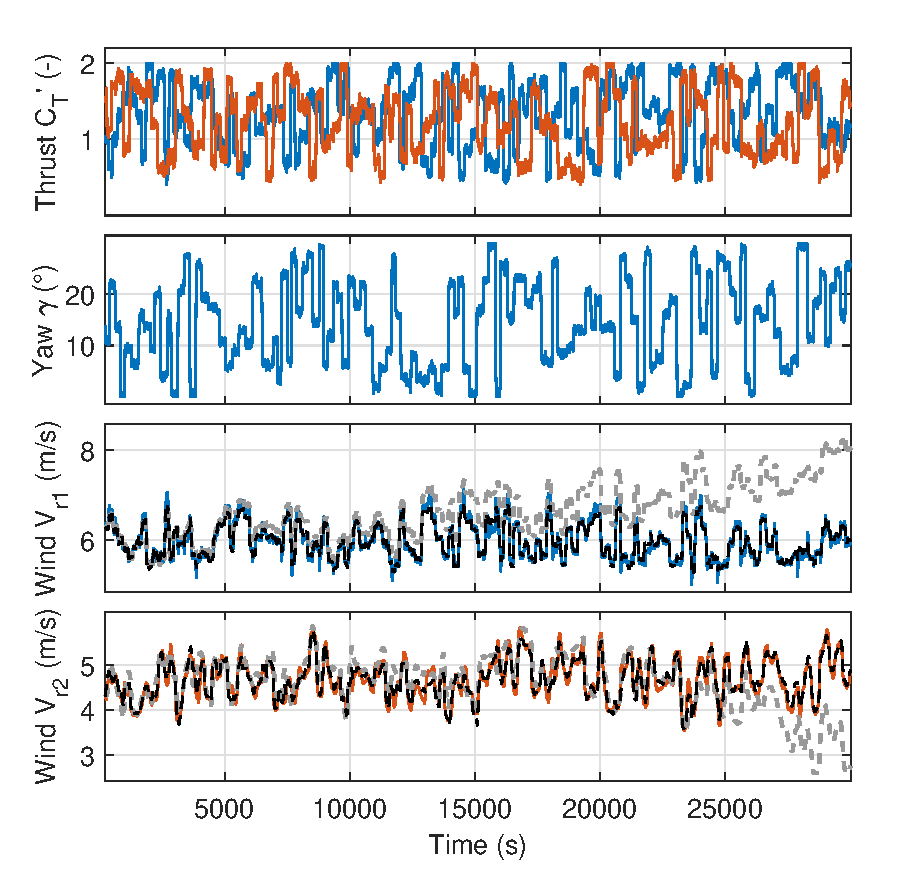
\includegraphics[width=0.485\textwidth]{figures/figures_IFAC23/03aFig_WRC_Id_Vr.eps}
        %\label{fig:WFSimgamma0}
    }
    \hfill
    \subfloat[Verification dataset with estimates $V_{r1}$ and $V_{r2}$;\; \;\; VAF~$V_{r1}/\,V_{r2}$:~$n_{\varphi}=21$: 93/\,85\%; $n_{\varphi}=6$: 90/18\%.]{
        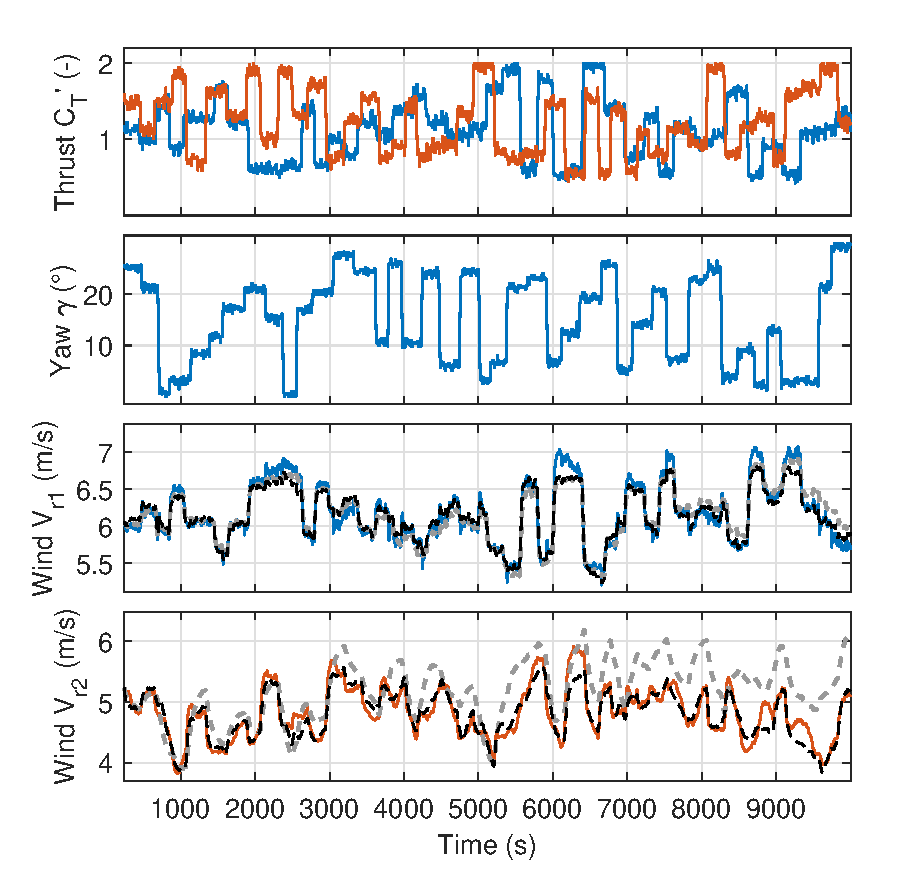
\includegraphics[width=0.485\textwidth]{figures/figures_IFAC23/03aFig_WRC_Val_Vr.eps}
        % \label{fig:PowerPerYaw}
    }\\
    \subfloat[Identification dataset with estimates $P_{\text{WF}}$;\; \;\;
    VAF~$P_{\text{WF}}$:~$n_{\varphi}=21$: 87\%; $n_{\varphi}=6$: 0\%.]{
        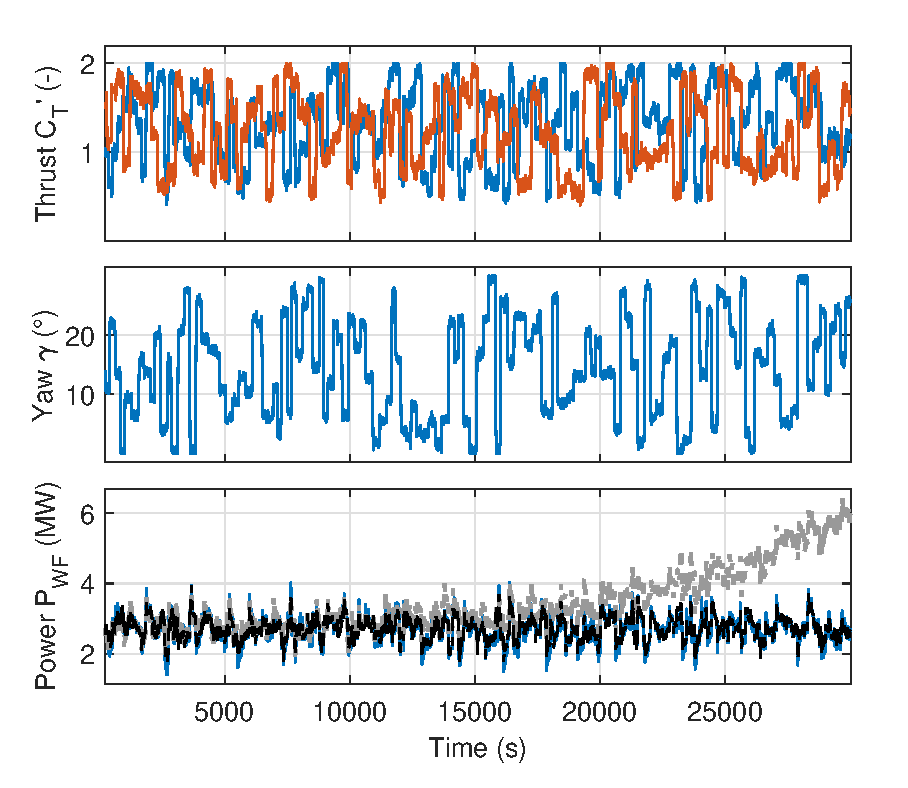
\includegraphics[width=0.485\textwidth]{figures/figures_IFAC23/03aFig_WRC_Id_P.eps}
        %\label{fig:WFSimgamma0}
    }
    \hfill
    \subfloat[Verification dataset with estimates $P_{\text{WF}}$;\; \;\; VAF~$P_{\text{WF}}$:~$n_{\varphi}=21$: 85\%; $n_{\varphi}=6$: 61\%.]{
        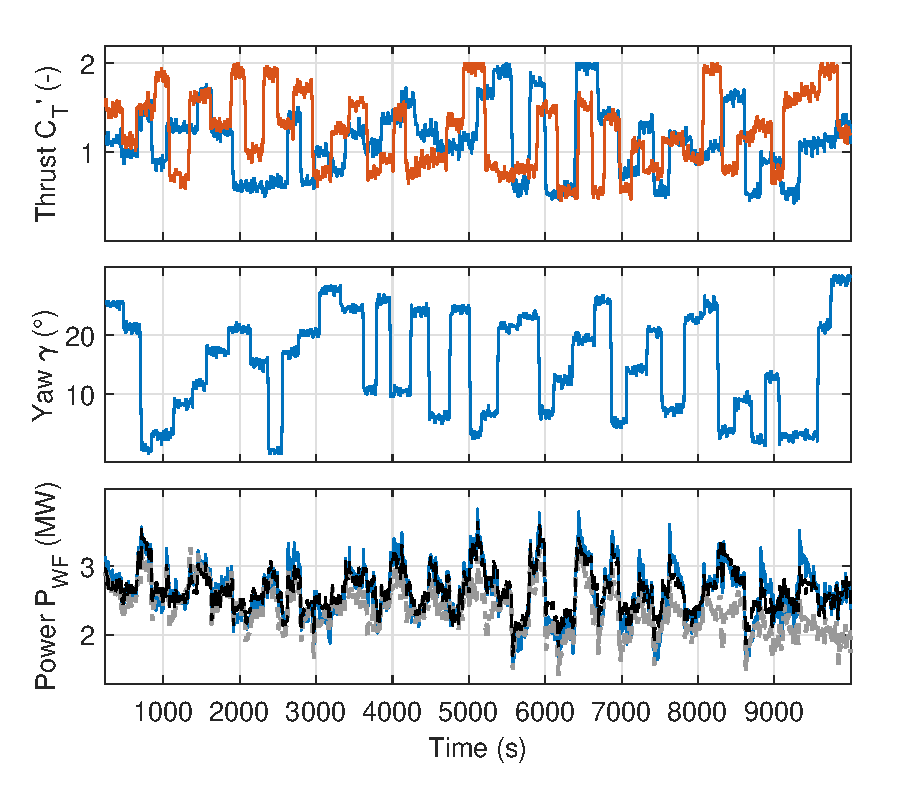
\includegraphics[width=0.485\textwidth]{figures/figures_IFAC23/03aFig_WRC_Val_P.eps}
        % \label{fig:PowerPerYaw}
    }
    \caption[Identification and verification datasets of the Koopman model for the WRC-AIC algorithm]{Identification (a, c) and verification (b, d) datasets of Koopman model $\hat{K}_2$ for the WRC-AIC algorithm: estimated effective wind speeds $V_{r1}$ and $V_{r2}$ (a, b) and farm power $P_{\text{WF}}$ (c, d). Subplots (top to bottom): thrust $C_T^\prime$; yaw $\gamma_1$; real vs. estimated $V_{r1}, V_{r2}$ (a, b) or $P_{\text{WF}}$ (c, d). WT1/WT2 signals are \mlBlue/\mlOrange, 21-state ($n_\varphi = 21$) and six-state  ($n_\varphi = 6$) model estimates are~\mlBlackDashed/\mlGrayDashed.}
    \label{fig:WRCAICOL_EDMD}
    
    % black and grey dashed lines denote the
\end{figure}
Note that the effective wind speed estimates are not used in the presented WRC-AIC design. However, they are included to demonstrate that, with the carefully designed new datasets, power predictions are as good as or even better than those of the effective wind speeds. Thus, the need for physics-based wind turbine models is eliminated in the presented design. The plots also illustrate the advantage of using the new set of lifted states. As before, the signals of the first and second turbines are depicted in blue and red, respectively, and the wind farm power is also shown in blue. Estimates obtained with the new linear Koopman model with 21 states are shown as black dashed lines, while those obtained with the old model are shown as grey dashed lines. With the new Koopman matrix, VAF values above 85\% are achieved for both datasets and all estimates. The black dashed lines closely follow the blue and red reference signals. However, when the new datasets are used with the old Koopman matrix from~\cite{dittmer2023koopman}, which includes only six states, considerable discrepancies develop over time between the reference signals and the estimates. This is attributed to the design of the six-state model, which includes the effective wind speeds and their quadratic and cubic terms but no temporal states to capture the evolution of the moving means, unlike the 21-state model, which includes the filtered control signals and the moving means as additional states. This also explains why, somewhat counterintuitively, the VAF values for the shorter verification datasets are higher than those of the identification sets. For the six-state model, apart from the least challenging case, the effective wind speed of the first turbine, for which a VAF value of 90.3\% is achieved, the verification VAF values remain low: 17.7\% for the effective wind speed of the second turbine and 60.6\% for the wind farm power. The VAF values for this comparison are summarized in Table~\ref{tab:WRCModelComparison}, which also includes the closed-loop results and is therefore placed in the section presenting the simulation results obtained with the MPC algorithms in closed loop.

Apart from the above described datasets, open-loop WFSim simulation results to quantify the effect of wake misalignment are obtained for a step-sweep of the yaw angle $\gamma_1$ from 0\textdegree{} to 35\textdegree{} with consecutive increases of 5\textdegree{} every 500 samples, resulting in a total of 4000 samples. During this sweep, the thrust control signals are set to their maximum value of 2 and the freestream wind is held constant at 8\,m/s. Figure~\ref{fig:OpenLoopResultsCombined} shows the resulting longitudinal wind field and the power output of the turbines and farm.
\begin{figure}[htb]
    \centering
    \subfloat[Longitudinal wind field for $\gamma_1$ at 0\textdegree{} and 20\textdegree{}.]{
        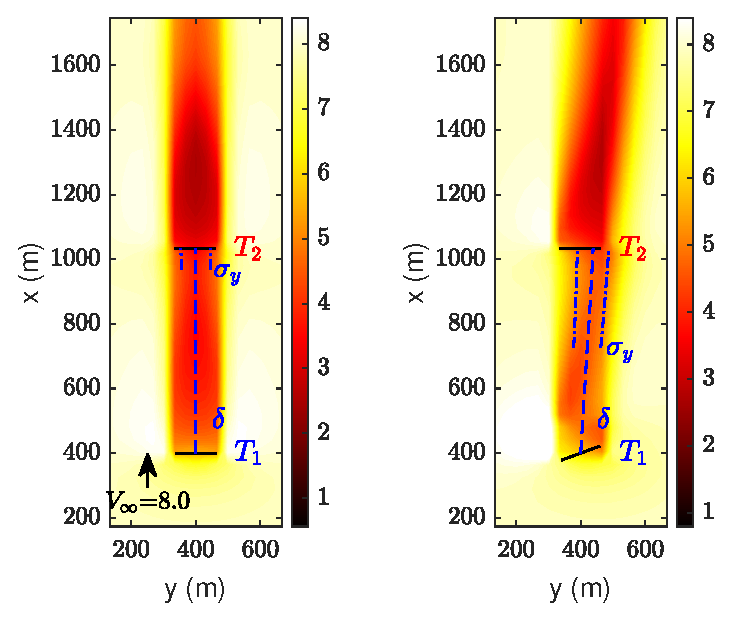
\includegraphics[width=0.48\textwidth]{figures/figures_IFAC23/03FigAngle0_20_tex.eps}
        \label{fig:WFSimgamma0}
    }
    \hfill
    \subfloat[Power $P_{\text{WF}}$ as a function of yaw angle $\gamma_1$.]{
        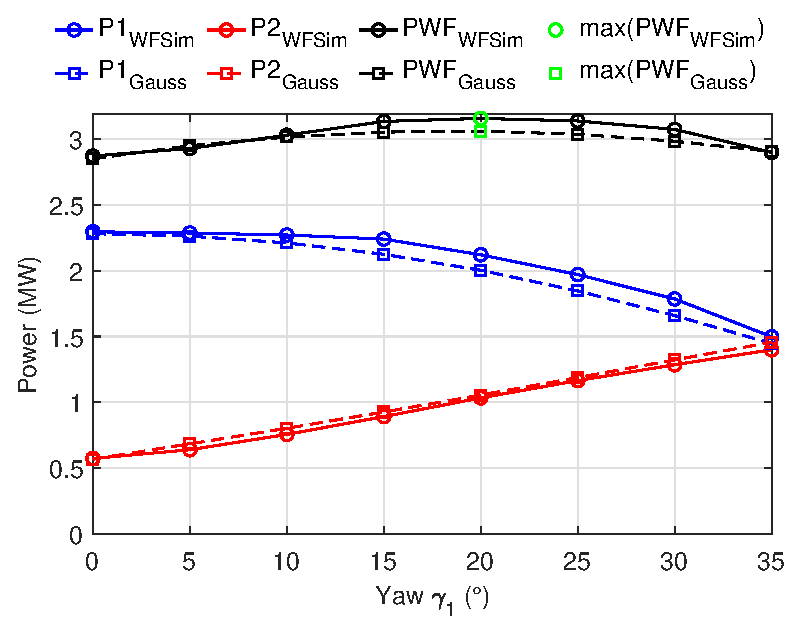
\includegraphics[width=0.48\textwidth]{figures/figures_IFAC23/01FigPwrVsYaw_tex.eps}
        \label{fig:PowerPerYaw}
    }
    \caption[Open-loop validation of the Gaussian wake model against WFSim.]{Open-loop validation of the Gaussian wake model against WFSim: (a) steady-state longitudinal wind field with Gaussian wake centerline $\delta$~(\mlOldBlueDashed) and expansion $\sigma_y$~(\mlOldBlueeDashDot); (b) power output comparison where WFSim results are marked with circles and the Gaussian model with squares: WT1 (\mlOldBlue), WT2 (\mlRed), total wind farm (\mBlack), and maximum power point (\mlOldGreen)}
    \label{fig:OpenLoopResultsCombined}
\end{figure}

Figure~\ref{fig:WFSimgamma0} visualizes the simulated longitudinal wind in steady state. The WFSim results, obtained by solving the 2D NSE \cite{boersma2018control}, are overlaid with the Gaussian wake model from \cite{bastankhah2016experimental}, with the centerline plotted as a blue dashed line and the far-field wake expansion as a blue dash-dotted line. The match of the wake expansion at the downstream rotor is reasonable. While the deflection angle of the Gaussian wake model in the far-wake region is slightly smaller than that of WFSim, the main area of speed deficit is nearly identical between the two. It should be noted that the wake centerline of a yawed turbine is curled in the near-wake region; therefore, modeling the centerline as a straight line in this region necessarily leads to discrepancies. This effect is addressed in more recent models such as the curled wake model \cite{martinez2019aerodynamics} or the Gaussian-Curl-Hybrid model \cite{king2020controls}, which have been shown to yield a better fit to large-eddy simulations and also report that the Gaussian model underestimates the power gain from wake steering. The standard Gaussian wake model is nevertheless used here for its simplicity, as it provides the optimal yaw angle with negligible computational effort.

Figure~\ref{fig:PowerPerYaw} shows the steady-state power at the end of each yaw step as a function of the yaw angle $\gamma_1$ for both WFSim and the Gaussian wake model. The power of the upstream turbine (blue) decreases as the yaw angle increases. This reduction is attributed to the reduced effective rotor area facing the wind and the inherent decrease in aerodynamic efficiency during yawed operation. These effects are analyzed in a comparative study of various yaw models \cite{sant2016comparing} and are further supported by recent field evaluations \cite{hulsman2022turbine}. Between 10\textdegree{} and 30\textdegree{}, the WFSim power of the first turbine slightly exceeds the Gaussian wake model prediction.

At farm level, the power increase due to WRC is 10\% in WFSim, compared to 6\% predicted by the Gaussian model. While this difference is non-negligible, the curves remain in close agreement, and both models identify the maximum farm power (green marker) at approximately 20\textdegree{} yaw, within the 5\textdegree{} resolution of the sweep. The matching location of the maximum and the similar curve shapes indicate that the Gaussian wake model is a computationally efficient and reasonable approximation of WFSim for determining the yaw angle in the combined controller, while the effective wind speeds for the thrust control are predicted with the Koopman model.

%\cite{boersma2019constrained}
% the deduction from the simulated wind fields

\subsubsection{Closed-Loop Results}
Figure~\ref{fig:ClosedLoopComparison} compares the closed-loop performance of the baseline AIC controller with the two WRC-AIC designs from Section~\ref{qLMPCDesign}, which combine yaw and thrust control.
\begin{figure}[!tbp]
    \centering
    \subfloat[Baseline AIC with fixed yaw ($\gamma_1 = 0^\circ$): TE 118.0\,kW, $1000\cdot$AA 6.2, VAF $P_{\text{WF}}$ 99.1\%.]{
        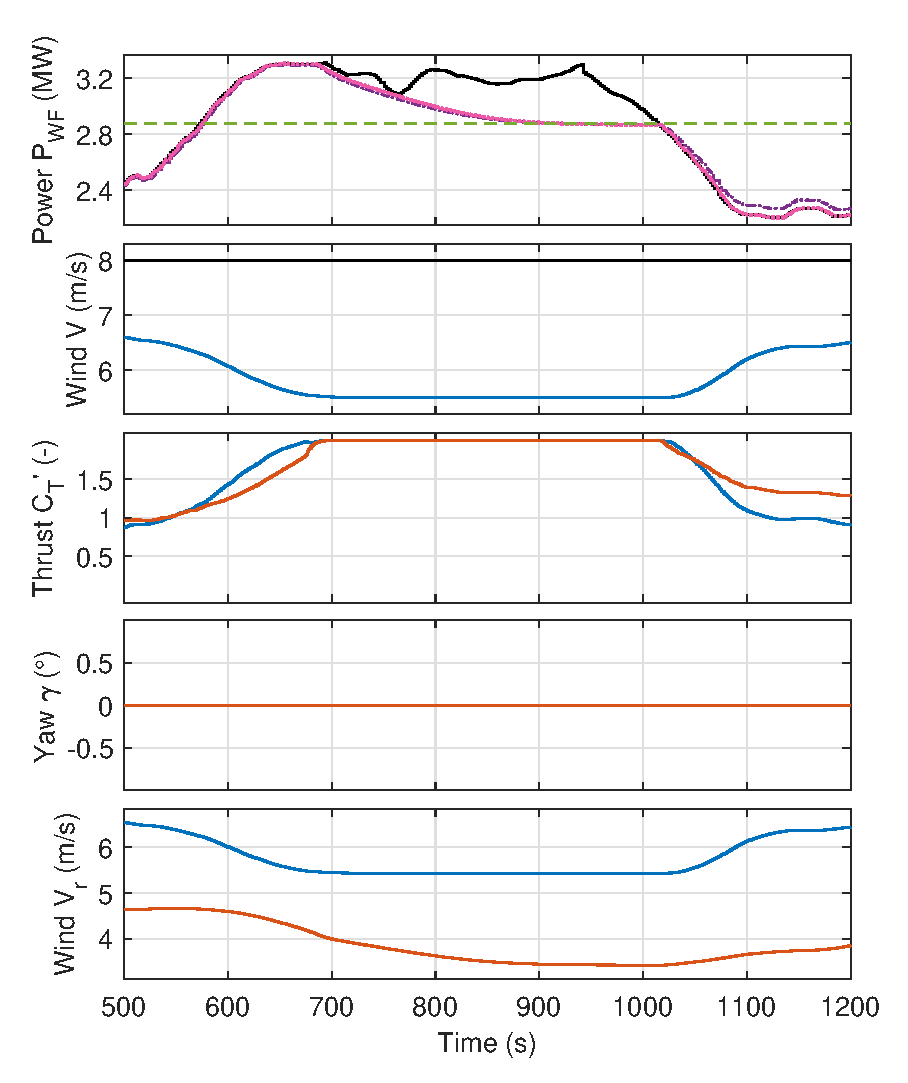
\includegraphics[width=0.48\textwidth]{figures/figures_IFAC23/04FigTimeSeries0_tex.eps}
        \label{fig:CLbaseline}
    }
    \hfill
    \subfloat[AIC with yaw set to the Gaussian-model optimum $\gamma_1^* = 18^\circ$ when $P_{\text{ref}} > P_{\text{greedy}}$:TE 65.3\,kW, $1000\cdot$AA 16.9, VAF $P_{\text{WF}}$ 99.1\%.]{
        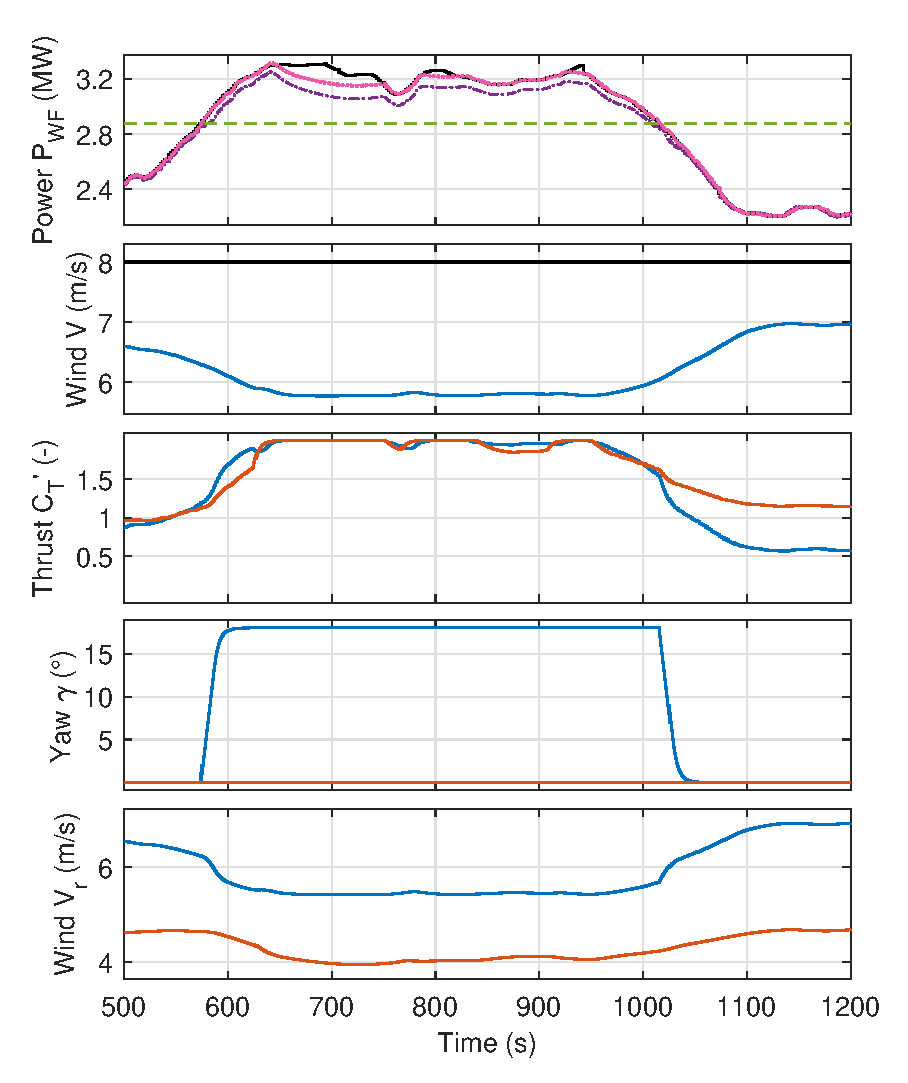
\includegraphics[width=0.48\textwidth]{figures/figures_IFAC23/05FigTimeSeriesQLMPC_tex.eps}
        \label{fig:CLMPC1}
    }
    
    \vspace{0.5cm}
    
    \subfloat[WRC-AIC, thrust and yaw controls optimized simultaneously: TE 27.8\,kW, $1000\cdot$AA 15.6, VAF $P_{\text{WF}}$ 99.9\%.]{
        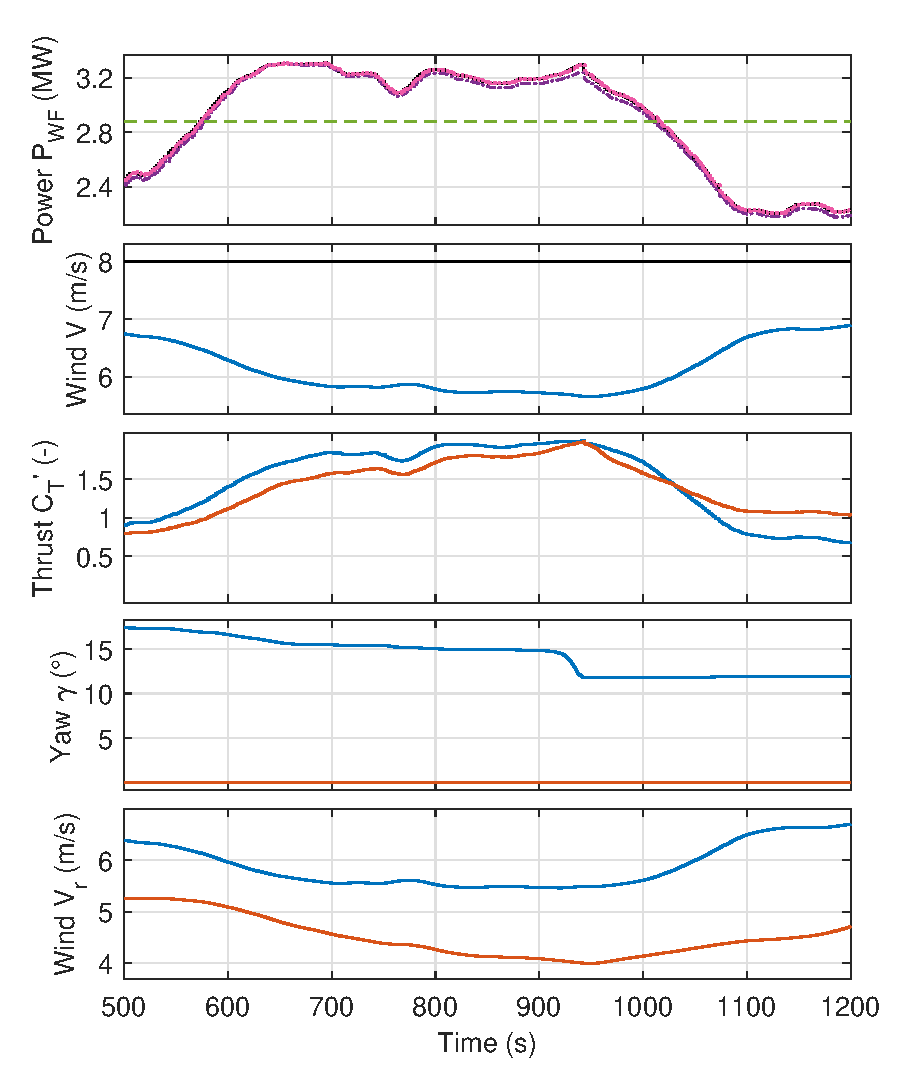
\includegraphics[width=0.48\textwidth]{figures/figures_IFAC23/06FigTimeSeriesLinMPC_tex.eps}
        \label{fig:CLMPC2}
    }
    
    \caption[Controller comparison Koopman MPC: baseline AIC and the two WRC-AIC algorithms]{Controller comparison Koopman MPC: baseline AIC and the two WRC-AIC algorithms; objectives mean tracking error (TE) and actuator activity (AA). Subplots (top to bottom): reference $P_{\text{ref}}$ (\mBlack), farm power $P_{\text{WF}}$ (\mlPurpleDashDot), predicted farm power $P_{\text{WF,est}}$ (\mlPinkDotted), and greedy power $P_{\text{greedy}}$ (\mlGreenDashed); wind speeds $V_\infty$ (\mBlack) and $V_1$ (\mlBlue); thrust $C'_T$; yaw $\gamma$; and effective wind speeds $V_{r1}, V_{r2}$. WT1/WT2 signals are \mlBlue/\mlOrange.}
    \label{fig:ClosedLoopComparison}
\end{figure}

The predicted farm power $P_{\text{WF,est}}$ is the estimate from $\hat{K}_2$ for the optimal inputs of the respective sample. It is the first element of the prediction trajectory, shown at the sample of the resulting farm power. The effective wind speeds are not estimated, as they are not used by the controller. The titles give tracking error (TE), the actuator activity multiplied by 1000 for easier readability ($1000\cdot$AA), and the VAF value of $P_{\text{WF,est}}$ for the plotted interval from $k = 500$ on. The weighting parameters are for all algorithms set to $Q = 10^{-4}$ and $R = 10^{-6}$. The weights on the changes of the control inputs are $R_{u1} = R_{u2} = 1$ for the thrust control signals and $R_{u3} = 0.1$ for the yaw angle in degrees, to keep the yaw changes roughly in the same order of magnitude as the thrust changes. Both TE and AA are computed as mean values over the evaluation period, with the AA including the respective weighting factors and a small penalty of $10^{-3}$ on the yaw angle. This penalty is not included in the QP for now, but is meant to indicate that less yaw misalignment is preferred.
%
The controllers are tasked with tracking a power reference signal, defined as:
\begin{align*}
    P_{\text{ref},k} = \big(a_{\text{const}} + a_{\delta} \, \delta P_k \big) P_{\text{greedy}},
\end{align*}
where $\delta P_k$ is a random sequence as in \cite{sharan2022Koopman}, and $P_{\text{greedy}}$ represents the maximum power production of the farm when both turbines operate at maximum thrust ($C_T' = 2$) and zero yaw ($\gamma = 0^\circ$). While the parameters in \cite{sharan2022Koopman} were set to $a_{\text{const}} = 0.8$ and $a_{\delta} = 0.35$, the present work uses $a_{\text{const}} = 0.9$ and $a_{\delta} = 0.25$, and the vector $\delta P$ has been resampled to update only every second time step. These modifications yield a reference trajectory that exceeds the greedy power for longer durations, thereby increasing the importance of wake steering for successful tracking. TE and AA are evaluated from $k = 500$ to the end of the simulation at $k = 1200$, the interval shown in Figure~\ref{fig:ClosedLoopComparison}, and from $k = 240$, i.e., after the start-up of the wake, so that initialization artifacts do not affect the performance metrics. The second interval additionally contains the samples from 240 to 500, in which the reference is below the greedy power. In the following, the values from $k = 240$ are given in brackets.

Figure~\ref{fig:CLbaseline} shows the performance of the baseline AIC scheme with the yaw angle fixed at zero. Figure~\ref{fig:CLMPC1} shows the results of the first WRC-AIC Koopman MPC algorithm with prescribed yaw, which sets the yaw angle to the optimum of the Gaussian wake model whenever the reference exceeds the greedy power. For the considered case, the optimum of the Gaussian model was found to be roughly $\gamma_1^* = 18^\circ$. Finally, Figure~\ref{fig:CLMPC2} shows the results of the second WRC-AIC Koopman MPC algorithm, which optimizes thrust and yaw simultaneously. The first plot in each subfigure shows the wind farm power $P_{\text{WF}}$, the power reference $P_{\text{ref}}$, and the greedy power $P_{\text{greedy}}$.

In Figure~\ref{fig:CLbaseline}, with the thrust coefficient as the only actuator, the farm power initially exceeds the greedy power when the reference demands it. However, it falls back to the greedy power once the increased wind speed deficit from the first turbine's higher thrust reaches the second turbine. In Figure~\ref{fig:CLMPC1}, the yaw angle is increased when the reference exceeds the greedy power, which reduces the tracking error by a factor of 1.8, from 118\,kW to 65.3\,kW, for the time samples from 500 to 1200. 
In Figure~\ref{fig:CLMPC2}, the tracking error is further reduced to 27.8\,kW by including the yaw angle as a third control input, i.e., by a factor of 2.3 compared with the prescribed yaw.

Similar to the adaptive AIC, the improved tracking performance comes at the cost of higher actuator activity: from sample 500 on, the AA of both WRC-AIC designs is more than twice that of the baseline AIC. This is expected, as the AA includes the yaw rate and, with a small weight of $10^{-3}$, the yaw angle itself, since yaw misalignment adds strain on the turbine. The AIC with static yaw changes the thrust less than the joint WRC-AIC, but operates at a larger yaw angle; with the yaw angle term, the joint WRC-AIC therefore also has the lower AA.

To assess the effect of the input features and the moving means, the analysis is repeated with a Koopman model with only the six lifted states used in \cite{dittmer2023koopman}, i.e., the effective wind speeds, their squares and cubes.


Table~\ref{tab:WRCModelComparison} summarizes the discussed WRC-AIC algorithms for the model with six lifted states and the 21-state model. The state matrix of the six-state model has two eigenvalues close to 1, the largest with an absolute value of 1.0002, and its open-loop simulations drift over the long datasets, resulting in VAF values of 0 for the identification dataset and between 17.7\% and 90.3\% for the verification dataset. In closed loop, where the prediction starts at every sample from the estimated effective wind speeds and only covers the horizon of 10 samples, the six-state model still performs reasonably well. However, the 21-state model reduces both the tracking error and the actuator activity for all three controllers, e.g., for the WRC-AIC from 36.9\,kW to 27.8\,kW and from $20.8 \cdot 10^{-3}$ to $15.6 \cdot 10^{-3}$. As discussed before, this model has one eigenvalue at 1 because of the bias state. The second largest eigenvalue of this discrete model is 0.9985, so the 21-state system is stable.


% Created by writeWRCModelTable (mainGeneratePlotThesis) on 2026-10-31
\begin{table}[htbp]
    \centering
    \caption[Input-only Koopman power models of the WRC-AIC]{Input-only Koopman power models of the WRC-AIC: VAF values of the effective wind speeds $V_{r1}$, $V_{r2}$ and farm power $P_{\text{WF}}$ for the identification and verification data, largest eigenvalue magnitude of $A$, and closed-loop tracking error TE and actuator activity AA from 500\,s onward (as in Figure~\ref{fig:ClosedLoopComparison}) and, in brackets, from sample 240 onward.}
    \label{tab:WRCModelComparison}
    \begin{tabular}{p{3.2cm} l l}
        \toprule
        Model & Criterion & Value \\
        \midrule
        \multirow{6}{=}{6 states}
        & VAF $V_{r1}$ / $V_{r2}$ / $P_{\text{WF}}$ (\%), Id.  & 0.0 / 0.0 / 0.0 \\
        & VAF $V_{r1}$ / $V_{r2}$ / $P_{\text{WF}}$ (\%), Val. & 90.3 / 17.7 / 60.6 \\
        & $\max|\lambda(A)|$                                   & 1.0002 \\
        & TE (kW) / AA ($10^{-3}$), baseline AIC               & 127.8 / 10.5 \; (111.3 / 10.5) \\
        & TE (kW) / AA ($10^{-3}$), AIC static yaw            & 72.0 / 20.3 \; (70.5 / 17.7) \\
        & TE (kW) / AA ($10^{-3}$), WRC-AIC                   & 36.9 / 20.8 \; (32.6 / 21.1) \\
        \midrule
        \multirow{6}{=}{21 states}
        & VAF $V_{r1}$ / $V_{r2}$ / $P_{\text{WF}}$ (\%), Id.  & 96.1 / 91.7 / 86.7 \\
        & VAF $V_{r1}$ / $V_{r2}$ / $P_{\text{WF}}$ (\%), Val. & 93.4 / 85.3 / 85.5 \\
        & $\max|\lambda(A)|$                                   & 0.9985 \\
        & TE (kW) / AA ($10^{-3}$), baseline AIC               & 118.0 / 6.2 \; (93.0 / 5.7) \\
        & TE (kW) / AA ($10^{-3}$), AIC static yaw            & 65.3 / 16.9 \; (54.5 / 13.5) \\
        & TE (kW) / AA ($10^{-3}$), WRC-AIC                   & 27.8 / 15.6 \; (29.7 / 15.0) \\
        \bottomrule
    \end{tabular}
\end{table}

%\input{figures/figures_IFAC23/tab_WRC_ModelComparison}


These results show that the Koopman-based WRC-AIC MPC effectively coordinates yaw and thrust to overcome the wake-induced limitations of AIC alone. The following section concludes the chapter by summarizing the main results and discussing the limitations and future research directions for Koopman-based wind farm control.


\section{Conclusions}
This chapter presented and analyzed EDMD and EIODMD applications using two sets of Koopman lifting functions for wind farm control. The focus of both studies was to improve the tracking error, defined as the mean absolute difference between grid demand and farm power output, under more challenging conditions than could be tested with the default settings in WFSim. The objective function optimized in both the adaptive AIC and the WRC-AIC schemes is a weighted sum of the squared tracking error and the change in actuator signals. The default weight values from WFSim were adopted: $Q = 10^{-4}$ for the tracking error and $R = 10^{-6}$ for the change in actuation (hereafter referred to as actuator activity). 

Section~\ref{sec:WindFarmSimulationWFSim} discussed the modifications required in the WFSim simulation environment to enable adaptive control testing and to investigate the influence of intentional yaw misalignment through a yaw-angle-dependent power coefficient. This was followed by the design, implementation, and evaluation of an adaptive AIC controller, alongside two WRC-AIC controllers combining wake redirection and axial induction control.

Section~\ref{sec:AdaptiveWindFarmqLMPCforAIC} discussed a data-driven EDMD algorithm. A state-space system was established incorporating the effective wind speeds of the two turbines, as well as their squares and cubes as lifted states, alongside the two turbine thrust controls. A test case featuring a wind speed ramp, followed by a corresponding increase in power demand, was established. It was found that an adaptive version of the AIC qLMPC successfully mitigated the impact of this wind speed change (which was absent from the EDMD training data), reducing the tracking error from $456.0\,\text{kW}$ to $17.2\,\text{kW}$, albeit with an increase in actuator activity from $3.8 \cdot 10^{-3}$ to $7.6 \cdot 10^{-3}$. 

In Section~\ref{sec:WindFarmLinearMPCforWRC-AIC}, a test case with constant wind was set up under a reference power trajectory exceeding the greedy power of the wind farm (i.e., the power produced when all turbines face directly into the wind). Two WRC-AIC algorithms and a baseline AIC were tasked with tracking this challenging reference trajectory. The baseline AIC exhibited a considerable offset due to insufficient power generation, resulting in a tracking error of $118.0\,\text{kW}$. An AIC algorithm utilizing an offline-optimized static yaw angle of $\gamma_1^* = 18^\circ$ reduced the tracking error to $65.3\,\text{kW}$. Meanwhile, the WRC-AIC algorithm, which optimized thrust and yaw jointly, further reduced the tracking error to $27.8\,\text{kW}$. 

While the baseline AIC resulted in the lowest actuator activity ($6.2 \cdot 10^{-3}$), the WRC-AIC achieved the lowest tracking error while increasing actuator activity only to $15.6 \cdot 10^{-3}$, compared to $16.9 \cdot 10^{-3}$ for the static yaw AIC. Because the original simulation weights were retained, the actuator rate penalty remained small relative to the tracking error weight, allowing rapid thrust adjustments without heavy penalization. This results in heightened actuator activity, which is most pronounced for the two designs with yaw control. A comprehensive sensitivity analysis of the quadratic program weights is left for future research.

Across the considered test cases, the tracking error ranged from just over $10\,\text{kW}$ to nearly $500\,\text{kW}$, while actuator activity varied between about $4 \cdot 10^{-3}$ and $2 \cdot 10^{-2}$. For the AIC algorithm, actuator activity consists solely of the two thrust signals, which range between $0.2$ and $2$. For the WRC schemes, the yaw angle was added as a control input, allowed to vary from $0^\circ$ to $22^\circ$ with an additional penalty of $0.1$ to keep it roughly in the same order of magnitude as the thrust signals. In short, the default WFSim configuration places a heavy emphasis on minimizing tracking error. However, setting $R$ to zero was found to induce instabilities. A thorough investigation into the influence of higher penalty values for actuator activity remains a direction for future research.

Apart from the comparison between non-adaptive and adaptive AIC schemes, Section~\ref{sec:AdaptiveWindFarmqLMPCforAIC} also provides a sensitivity study on the two tuning parameters of the adaptive scheme, the update trigger condition and the sample size of historic data that is useful to be included in an update of the Koopman matrix. It was found that setting the trigger condition to 0.15\,m/s was a good compromise between tracking error and number of model updates. The value of this trigger number corresponds to the difference between historic wind predictions and measurements for the first turbine. As this can be very well predicted as long as the wind stays constant it was a reliable indicator of a change in freestream wind. It was also found that five samples of historic effective wind speed measurement, here estimated from the turbine power, needed to calculate the Koopman matrix update. Doubling or quadrupling that trajectory length however resulted in performance degradation rather than improvements. Batch lengths below five samples remain to be investigated. An excitation signal was included during consecutive updates. Changing the influence weight of that signal, which is currently added with a weight of 0.01 to the control signal weighted with 0.99, as well as changing its form, or including a forgetting factor to put more weight on more current measurements is another research direction. Another very obvious area of research would be investigating the influence of additional lifting functions, other than the already included squares and cubes of the effective wind speed.


In Section~\ref{sec:WindFarmLinearMPCforWRC-AIC}, the improvement in tracking error depending on including a total of~21 carefully selected lifting functions is discussed in detail. The aforementioned lifted states, the effective wind speeds, their squares and cubes form six lifted states. The following types of lifting functions are used to form an additional set of 14 lifted states: \begin{itemize}
    \item the three inputs are included as states in filtered form to keep the model linear and 
    \item four additional features represent the influence of the controls on the turbine power. 
    \item Additionally, there are four moving means that are used to include the long time delays of approximately 100\,s that occur for the two turbines spaced more than 600\,m apart and 
    \item three products of these means and the feature representing the power harvest at the second turbine.
\end{itemize}
An offset or bias state is added as the 21st state. This was previously not necessary, as one wind speed in front of the first turbine was used for prediction, but became necessary with this prediction depending only on the control inputs. This has the advantage that it emulates real wind farm control better, where reliable wind measurements might not be available. 

The inclusion of WRC led to an increase in total
farm power output exceeding 5\% for all simulations used: the Bastankhah analytical wake model predicted
an improvement of approximately 6\%, while the WFSim simulation indicated an increase of
around 10\%. These results are consistent with trends reported in related literature. Both the
Bastankhah and the NSE-based WFSim models showed good agreement in
terms of wake expansion and power prediction. The combination of increased power yield and
a good representation of the wind farm dynamics with the data-driven Koopman model resulted in accurate power reference tracking, even for reference
signals exceeding the greedy power. This result highlights the potential of Koopman-based
WRC-AIC control strategies to enhance wind farm efficiency and support grid stability through power delivery more closely following the demanded power.
    \chapter{Conclusions and Outlook} \label{Conclusions}
This thesis has shown that predictive control based on qLPV models is fast enough for real-time wind turbine control and improves power reference tracking compared to established baseline schemes. Furthermore, it was demonstrated that Koopman-based MPC algorithms achieve smooth power reference tracking in wind farm control. Section~\ref{sec:Conclusions} summarizes these results, and Section~\ref{sec:Outlook} discusses resulting directions for future research.
\section{Conclusions}\label{sec:Conclusions}
This dissertation develops qLPV, structured low-order and data-driven control schemes for wind energy conversion systems at the turbine and wind farm levels. The aim is to minimize the Levelized Cost of Energy (LCoE) of increasingly large and slender turbines in dense wind farms by balancing power yield, actuator usage, and mechanical loads. For turbine control, velocity-based qLMPC handles the nonlinearity of the turbine models. For farm control, data-driven MPC based on Koopman operator theory is used, as the high-dimensional ODEs of the discretized flow equations prevent real-time physics-based MPC. All algorithms are real-time capable, with mean computation times well below the typical turbine controller sample time of about 10\,ms.

One contribution of this thesis is the derivation of qLPV wind turbine models with a good fit relative to FAST in the range of 0.1\,Hz to 0.7\,Hz, which is relevant for turbine control. Two models are designed, a 5th order qLPV model with rotor and tower dynamics, and a 9th order model containing additionally blade out-of-plane, generator and slip angle states. The latter fits better in open loop but brings only marginal closed-loop gains. It was nevertheless chosen as the qLMPC plant, as it causes no measurable computational penalty and contains a subset of states close to an established prediction model \cite{Bianchi2007}; for the application to FAST, the prediction model was extended to all its states except the tower side-to-side motion. The velocity-based MIMO qLMPC was benchmarked against a collective pitch and torque SISO baseline, together with Individual Pitch Control (IPC) and aerodynamically modeled Trailing Edge Flap Control (TEFC); all configurations maintain the mean power. Without model mismatch, the qLMPC reduces the standard deviations of the tower fore-aft acceleration and the power tracking error by factors of up to 4.1 and 11.4. On FAST, the adapted designs still reduce the power fluctuations by a quarter to a third, which no other approach achieves, but increase the tower Damage Equivalent Load (DEL) and do not reduce the blade DEL. IPC and the combined IPC-TEFC, referred to as Active Aerodynamic Load Control (AALC), reduce the blade DEL above rated by 21\% to 24\% on the optimization and two verification datasets with gains optimized at a single wind speed, AALC at a considerably lower pitch actuator power. Only the combinations of qLMPC and IPC reduce both the blade DEL and the power fluctuations. These results underline the potential of qLMPC, but also its dependence on an accurate representation of the wind acting on the rotor and of the turbine dynamics.

At the farm level, this thesis introduces a data-driven adaptive Axial Induction Control (AIC) in WFSim, based on Koopman operator theory: the model is identified via Dynamic Mode Decomposition and physics-inspired lifting functions. It estimates the effective wind speeds and tracks power references that a non-adaptive scheme trained on the same, deliberately incomplete dataset cannot reach. Updating the model only when significant discrepancies are detected reduces the tracking error from 456\,kW to 17.2\,kW, with a Variance-Accounted-For of the effective wind speed of nearly 100\% for the upstream turbine and of about 80\% in open loop and 98\% in closed loop for the downstream turbine. Combined Wake Redirection Control (WRC) and AIC was explored in two ways: pre-optimizing the yaw misalignment with the Bastankhah-Gaussian wake model, and a WRC-AIC Koopman MPC optimizing thrust and yaw jointly. With a linear Koopman model lifted by filtered control signals, nonlinear control features and moving means, and using only the measured turbine powers, the joint optimization reduces the tracking error for power references above the greedy power from 118\,kW with baseline AIC and 65.3\,kW with pre-optimized yaw to 27.8\,kW, showing that data-driven models can capture the physical effects to optimize the farm yield.
\section{Outlook} \label{sec:Outlook}
%Future research can follow three directions: bringing the simulation models and the evaluation closer to reality, validating the controllers in field tests, and investigating neural network-based models.

Despite the promising results, several idealized assumptions within the simulation framework must be addressed to transition to real-world application. The individual turbine simulations assume that the wind at the turbine is perfectly known. While wind estimators are routinely used in industry \cite{soltani2013estimation}, their accuracy is inherently sensitive to turbine parameters that inevitably change as the system ages: uncertainty in the power coefficient, for example, biases the estimated rotor-effective wind speed \cite{brandetti2022ill}. Sensors such as spinner anemometers and lidar offer an alternative. The assumption of a perfectly known current wind speed is optimistic, whereas not using any wind preview is pessimistic: with lidar preview, both controllers in \cite{schlipf2012comparison} considerably reduce the tower DEL compared to a baseline feedback controller, whereas the qLMPC in this thesis, using only the current wind speed, increases it on FAST. Future work should therefore explore lidar-based wind preview to enhance MPC schemes for both Collective Pitch Control and IPC, particularly for gust alleviation.
%
Moreover, the application of the qLMPC to FAST showed that its tower load reduction is lost, probably because of the single-point wind speed used for scheduling, while the rotor averages a full wind field, and because of dynamics above about 0.7\,Hz that are not contained in the prediction model. That model mismatch limits the advantage of MPC is also suggested by \cite{schlipf2012comparison}, where a simple feedforward controller combined with collective pitch and tower feedback performs slightly better than a nonlinear MPC based on a reduced model, although its additional tower feedback also contributes. A further source of model mismatch is the actuator model: the pitch and generator torque dynamics are modeled as first-order transfer functions with constant parameters. In practice, these actuator responses degrade over time, so that learning and adapting to changed actuator behavior is a necessary research extension. 
%
The wind farm studies considered a wind speed ramp and constant inflow without turbulence. While the adaptive AIC presented here was shown to be adequate to address this task, the constant forgetting factor could be replaced by the matrix forgetting factor used for Koopman-based MPC in \cite{calderon2023data}. The results presented in~\cite{dittmer2026koopman} extend the WFSim environment to support turbulent inflow using the Kaimal Normal Turbulence Model, demonstrating that while turbulence reduces the potential gains from WRC compared to steady-state predictions, the combined WRC-AIC scheme still outperforms baseline AIC, reducing power tracking error considerably under realistic, time-varying wind conditions. Closed-loop WRC in this work relies on the measured turbine powers only, but load-based wake tracking could provide the wake position as an additional feedback signal. Such load-based estimates were validated against scanning lidar measurements in a field test in \cite{onnen2026field}.
%
The load evaluation under WRC-induced yaw misalignment remains an open problem, which cannot be addressed with WFSim's actuator disk turbine model. This quasi-static turbine model, which represents the turbine as an energy sink without mechanical dynamics apart from a first-order filter on the thrust control signal, is also not capable of imitating the dynamic behavior required to fully evaluate power demand following. Transitioning to environments such as FAST.Farm would allow for the inclusion of dynamic turbine behavior, a comprehensive evaluation of loads during WRC, and the investigation of Dynamic Induction Control alongside AIC and WRC. Furthermore, the framework should be tested on a higher number of turbines under realistic, varying wind directions.
%
The evaluation of the controllers should also become more realistic. Another research opportunity lies in defining a concrete financial advantage for load alleviation against the disadvantage of increased actuator wear. Quantifying this trade-off is essential for minimizing the LCoE with a commercially viable controller, see, e.g., \cite{pusch2024impact}. The actuator power criterion used in this thesis is only a proxy for actuator wear: full-scale tests of blade bearings show that the wear caused by IPC depends strongly on the bearing design, the lubrication, and lubrication runs, and that tests with static loads can be harsher than those with dynamic loads \cite{bartschat2023effect}.

To prove industrial validity, the controllers should ultimately be validated with measurement data. Research wind farms such as WiValdi, operated by the German Aerospace Center (DLR) together with its partners in the Research Alliance Wind Energy, provide the required instrumentation: inflow measurements from meteorological masts and lidar, together with load measurements on instrumented turbines, would allow both the effective wind speed estimates and the load reductions predicted here to be verified experimentally.

Independently of these steps, neural network-based models offer a promising alternative for the data-driven farm control. The physically motivated lifting functions selected in this thesis were shown to yield accurate Koopman models for wind farm control. Subsequent work~\cite{sharan2024autoencoder, sharan2026tcn}, to which the author contributed, has explored neural network-based lifting functions, suggesting that learned lifting functions can outperform manually selected ones. This direction is promising for larger farms and more complex inflow, where overlapping wakes, direction-dependent interactions, and varying transport delays make suitable lifting functions hard to select based on physical insight. As the MPC acts on the lifted model, learned lifting functions are part of the control law. While the input constraints remain satisfied, guaranteeing safe behavior of the predicted states is difficult as long as the behavior of the network outside its training data cannot be bounded.

%The results highlight the potential of physics-based and data-driven predictive multivariable control for the increasingly complex trade-offs in wind energy production.
    \appendix
    \include{chapters/document}
   
   % 
    \bibliography{chapters/myLiterature_with_dois}
    
    \cleardoublepage
  %  \pagenumbering{Roman}              % restart as I, II, III...
 
 %    \include{chapters/publications}
     \chapter*{Curriculum Vitae}
\phantomsection
\addcontentsline{toc}{chapter}{Curriculum Vitae}
\markboth{Curriculum Vitae}{Curriculum Vitae}
\noindent\textbf{\large Antje Dittmer} \large  n\'ee Paulmann \normalsize born 27 September 1980 in Wedel, Germany, German citizen
\bigskip

\large Education\\[-8pt]
\noindent\rule{15.25cm}{0.4pt}\\[3pt]
\normalsize
\begin{tabular}{@{}p{3.2cm}p{11.3cm}@{}}
    08/1987--06/1991 & Grundschule Iserbarg, Hamburg, Germany. \\[5pt]
    08/1991--06/2000 & Gymnasium Rissen, Hamburg, Germany %\\ &
    (Abitur). \\ [5pt]
    10/2000--10/2005 & Hamburg University of Technology, Germany, % \\ &
    General Engineering Science (Bachelor of Science, 03/2004) and 
    Electrical Engineering (Diplom-Ingenieurin, 10/2005). \\[34pt]
    since 12/2019 & Hamburg University of Technology, Germany, Institute of Control Systems,
    external doctoral candidate.
\end{tabular}

\bigskip
\large Selected Student Employment and Internships\\[-8pt]
\noindent\rule{15.25cm}{0.4pt}\\[3pt]
\normalsize
\begin{tabular}{@{}p{3.2cm}p{11.3cm}@{}}
    06/2002--08/2002 &  ESW - Extel Systems Wedel, Germany, Intern. \\[5pt]
    10/2002--07/2003 &  Hamburg University of Technology, Germany, Institute of Mathematics,  %\\ &
    Tutor. \\[18pt]
    10/2003--08/2005 & Airbus:~Student Employee in Hamburg, Germany (10/2003--07/2004 and 02/2005--08/2005) and Intern in Toulouse, France (09/2004--12/2004).\\
\end{tabular}

\bigskip
\large Employment History\\[-8pt]
%\noindent\rule{\linewidth}{0.4pt}\\[3pt]
\noindent\rule{15.25cm}{0.4pt}\\[3pt]
\normalsize
\begin{tabular}{@{}p{3.2cm}p{11.3cm}@{}}
    10/2005--01/2007 & The MathWorks, Munich, Germany, %\\ &
    Support Engineer. \\[5pt]
    02/2007--01/2008 &  Braunschweig University of Technology in cooperation with the German Aerospace Center, Germany,  Research Associate. \\[18pt]
    02/2008--12/2010 & German Aerospace Center, Braunschweig, Germany, %\\  &
    Research Associate. \\[18pt]
    01/2011--07/2012 & Parental and Family Leave. \\[5pt]
    08/2012--02/2015 & AOL Platforms, Palo Alto, CA, USA, %\\ &
    Research Engineer. \\[5pt]
    03/2015--01/2016 & Yahoo!, Sunnyvale, CA, USA, % \\ &
    Research Engineer. \\[5pt]
    03/2016--01/2020 & The MathWorks, Munich, Germany, %\\ &
    Senior Technical Consultant. \\[5pt]
    since 02/2020 & German Aerospace Center (DLR), Braunschweig, Germany, %\\
    Research Associate. \\
\end{tabular}
\end{document}          
